\documentclass[14pt, a4paper]{extreport}
\setcounter{secnumdepth}{3}

% Configure the page layout
\usepackage[
  a4paper,
  right=25mm,
  left=25mm,
  inner=35mm,
  outer=20mm,
  top=20mm,
  bottom=20mm, 
  twoside
]{geometry}

% Set font family
\usepackage[T1]{fontenc}
\usepackage{charter}

% Vietnamese language support
\usepackage[vietnamese]{babel}

% Insert images
\usepackage{graphicx}
\usepackage{float}
\usepackage[export]{adjustbox}
\graphicspath{{images/}}

% Insert hyperlinks
\usepackage{hyperref}

% Support more flexible table
\usepackage{tabularx}
\usepackage{array}
\usepackage{longtable}
\usepackage{makecell, cellspace, caption}

% Support enumeration and itemization
\usepackage{enumitem}

% Provides advanced math environments and features
\usepackage{amsmath}

% Support for algorithm
\usepackage{algorithm}
\usepackage{algpseudocode}

% Define line spacing
\usepackage{setspace}
\onehalfspacing

% Create graphic elements in LaTeX
\usepackage{tikz}

% Define commands for general information
\newcommand{\thesisname}{Hệ thống uy tín phục vụ xác thực hồ sơ và đánh giá kỹ năng}
\newcommand{\instructor}{PGS. TS. Nguyễn Đình Thúc}
\newcommand{\studentone}{Nguyễn Hải Tuyên - 21127474}
\newcommand{\studenttwo}{Trần Minh Đạt - 21127570}

% Blank page without page number
\newcommand{\blankpage}{
  \clearpage
  \thispagestyle{empty}
  \hfill
  \clearpage
}

% Blank page with page number
\newcommand{\emptypage}{
  \clearpage
  \hfill
  \clearpage
}

% Define column types for tables
\newcolumntype{L}[1]{>{\raggedright\let\newline\\\arraybackslash\hspace{0pt}}m{#1}}
\newcolumntype{C}[1]{>{\centering\let\newline\\\arraybackslash\hspace{0pt}}m{#1}}
\newcolumntype{R}[1]{>{\raggedleft\let\newline\\\arraybackslash\hspace{0pt}}m{#1}}

\begin{document}

\newgeometry{top=20mm,bottom=20mm}

\begin{titlepage}
  \begin{center}
    % Draw border with a small margin using TikZ
    \begin{tikzpicture}[remember picture, overlay]
      \draw[line width=2pt]
      ([xshift=15mm,yshift=-15mm]current page.north west)
      rectangle
      ([xshift=-15mm,yshift=15mm]current page.south east);
    \end{tikzpicture}

    {\large \textbf{ĐẠI HỌC QUỐC GIA THÀNH PHỐ HỒ CHÍ MINH}} \\
    \smallskip
    {\large \textbf{TRƯỜNG ĐẠI HỌC KHOA HỌC TỰ NHIÊN}} \\
    \medskip
    KHOA: CÔNG NGHỆ THÔNG TIN \\[1.8cm]

    {\Large \bfseries \studentone} \\
    {\Large \bfseries \studenttwo} \\[2cm]

    {\huge \bfseries HỆ THỐNG UY TÍN \\ PHỤC VỤ XÁC THỰC HỒ SƠ \\[3mm] VÀ ĐÁNH GIÁ KỸ NĂNG} \\[2cm]

    {\large KHÓA LUẬN TỐT NGHIỆP CỬ NHÂN} \\
    {\large CHƯƠNG TRÌNH CHẤT LƯỢNG CAO} \\[2cm]

    {\Large \textbf{GIẢNG VIÊN HƯỚNG DẪN}} \\
    \medskip
    {\large \instructor} \\

    \vfill
    \textit{Tp. Hồ Chí Minh, tháng 8 năm 2025}
  \end{center}
\end{titlepage}

\restoregeometry

\blankpage

\begin{titlepage}
  \begin{center}
    {\large \textbf{ĐẠI HỌC QUỐC GIA THÀNH PHỐ HỒ CHÍ MINH}} \\
    \smallskip
    {\large \textbf{TRƯỜNG ĐẠI HỌC KHOA HỌC TỰ NHIÊN}} \\
    \medskip
    KHOA: CÔNG NGHỆ THÔNG TIN \\[2cm]

    {\Large \bfseries \studentone} \\
    {\Large \bfseries \studenttwo} \\[2cm]

    {\huge \bfseries HỆ THỐNG UY TÍN \\ PHỤC VỤ XÁC THỰC HỒ SƠ \\[3mm] VÀ ĐÁNH GIÁ KỸ NĂNG} \\[2cm]

    {\large KHÓA LUẬN TỐT NGHIỆP CỬ NHÂN} \\
    {\large CHƯƠNG TRÌNH CHẤT LƯỢNG CAO} \\[2cm]

    {\Large \textbf{GIẢNG VIÊN HƯỚNG DẪN}} \\
    \medskip
    {\large \instructor} \\

    \vfill
    \textit{Tp. Hồ Chí Minh, tháng 7 năm 2025}
  \end{center}
\end{titlepage}

\blankpage

\begin{abstract}
Sự phát triển nhanh chóng của giáo dục trực tuyến đặt ra nhu cầu cấp thiết về các cơ chế đánh giá kỹ năng một cách minh bạch, khách quan và có thể xác minh được. 
Đáp ứng yêu cầu đó, đề tài này giới thiệu SkillChain -- một nền tảng phi tập trung ứng dụng công nghệ blockchain nhằm quản lý, đánh giá và tuyển dụng dựa trên kỹ năng thực tế của người học. 
Hệ thống sử dụng các hợp đồng thông minh để ghi nhận và xác thực các hành vi đóng góp, giải quyết thử thách, đánh giá và kiểm duyệt của người dùng, từ đó xây dựng hồ sơ uy tín minh bạch và không thể giả mạo. 
Ngoài ra, SkillChain còn tích hợp cơ chế tuyển dụng cho phép nhà tuyển dụng tìm kiếm ứng viên thông qua hồ sơ uy tín đã được xác minh trên chuỗi. 
Kết quả đạt được bao gồm một nguyên mẫu hệ thống đầy đủ chức năng, triển khai lưu trữ dữ liệu kết hợp on-chain và off-chain, cơ chế phân quyền dựa trên điểm uy tín, và giao diện người dùng trực quan hỗ trợ đầy đủ các vai trò. 
Đề tài đồng thời chỉ ra những hạn chế còn tồn tại và đề xuất các hướng phát triển để cải thiện chất lượng hệ thống trong tương lai.
\end{abstract}

\blankpage

\setcounter{page}{7}

\chapter*{Lời cảm ơn}

Để hoàn thành khóa luận tốt nghiệp, chúng tôi xin chân thành gửi lời cảm ơn đến Khoa Công nghệ thông tin, các bộ môn cùng toàn thể quý thầy cô giảng viên Trường Đại học Khoa học Tự nhiên -- Đại học Quốc gia Tp. Hồ Chí Minh 
đã tận tình giảng dạy, truyền đạt kiến thức và tạo điều kiện thuận lợi cho chúng tôi trong suốt quá trình học tập và nghiên cứu.

Đặc biệt, chúng tôi xin bày tỏ lòng biết ơn sâu sắc đến thầy Nguyễn Đình Thúc, người đã trực tiếp hướng dẫn và đồng hành cùng chúng tôi trong suốt quá trình thực hiện đề tài \textit{\thesisname}. 
Thầy không chỉ hỗ trợ chuyên môn, định hướng rõ ràng, mà còn luôn tận tâm động viên và giúp đỡ chúng tôi vượt qua những khó khăn trong quá trình nghiên cứu.

Dù đã nỗ lực hết mình để hoàn thiện khóa luận, nhưng do hạn chế về mặt thời gian và kinh nghiệm, bài làm không thể tránh khỏi những thiếu sót. 
Chúng tôi rất mong nhận được những góp ý quý báu từ quý thầy cô trong Hội đồng bảo vệ khóa luận để có thể hoàn thiện đề tài tốt hơn.

Một lần nữa, chúng tôi xin trân trọng cảm ơn tất cả quý thầy cô đã nhiệt tình giảng dạy, hỗ trợ và đồng hành cùng chúng tôi trong suốt quá trình học tập và thực hiện khóa luận này.

\emptypage

\chapter*{Đề cương chi tiết}
\addcontentsline{toc}{chapter}{Đề cương chi tiết}

\renewcommand{\thesection}{\arabic{section}}

\section{Thông tin chung}

\begin{itemize}[label = {}]
  \item \textbf{Giảng viên hướng dẫn:}
        \begin{itemize}
          PGS.TS. Nguyễn Đình Thúc
        \end{itemize}{}
  \item \textbf{Nhóm sinh viên thực hiện:}
        \begin{enumerate}
          \item Nguyễn Hải Tuyên (MSSV: 21127474)
          \item Trần Minh Đạt (MSSV: 21127570)
        \end{enumerate}
  \item \textbf{Loại đề tài:} Ứng dụng
  \item \textbf{Thời gian thực hiện:} Từ 3/2025 đến 8/2025
\end{itemize}

\section{Nội dung thực hiện}

\subsection{Giới thiệu về đề tài}

Trong quá trình tuyển dụng nguồn nhân lực hiện nay đối với các ngành nghề, đặc biệt là Công nghệ thông tin,
việc xác thực trình độ học vấn, kỹ năng và kinh nghiệm của một cá nhân vẫn còn gặp nhiều khó khăn.
Hiện nay, các nhà tuyển dụng và doanh nghiệp thường dựa vào chứng chỉ, bằng cấp hoặc thông tin do ứng viên cung cấp để đánh giá năng lực.
Tuy nhiên, những thông tin này \textbf{có thể bị làm giả} hoặc không phản ánh chính xác thực lực của ứng viên.

Bên cạnh đó, nhiều cá nhân có kỹ năng thực tế nhưng lại không có cách nào để chứng minh năng lực của mình ngoài những hồ sơ truyền thống.
Điều này làm hạn chế cơ hội phát triển và nâng cao giá trị cá nhân trong ngành.
Vì vậy, cần có một giải pháp minh bạch, khách quan và đáng tin cậy để xác thực trình độ của mỗi cá nhân,
đồng thời giúp doanh nghiệp dễ dàng đánh giá năng lực của ứng viên một cách chính xác hơn.

Theo đó, ý tưởng về một \textbf{Hệ thống uy tín phục vụ xác thực hồ sơ và đánh giá kỹ năng} được phát triển dựa trên công nghệ blockchain,
cung cấp một nền tảng giúp cá nhân có thể chứng minh năng lực của mình một cách minh bạch, công khai và không thể thay đổi.
Hệ thống cho phép người dùng tham gia các thử thách để kiểm tra và chứng minh kỹ năng, đồng thời áp dụng cơ chế đánh giá phi tập trung để đảm bảo tính khách quan.

Thay vì chỉ dựa vào văn bằng, chứng chỉ hay lời khai của ứng viên, hệ thống này sẽ ghi nhận kết quả đánh giá được tích lũy lên blockchain và dịch vụ lưu trữ phi tập trung,
giúp tạo ra một hồ sơ uy tín đáng tin cậy, có thể sử dụng trên nhiều nền tảng khác nhau.
Cộng đồng chuyên gia và nhà tuyển dụng có thể tham gia vào quá trình đánh giá để đảm bảo chất lượng,
đồng thời giúp thúc đẩy sự phát triển của một hệ sinh thái xác thực năng lực trong lĩnh vực Công nghệ thông tin.

\subsection{Mục tiêu đề tài}

Đề tài nhằm xây dựng một hệ thống uy tín phi tập trung ứng dụng công nghệ blockchain để xây dựng và xác thực kỹ năng và hồ sơ cá nhân, bước đầu giới hạn trong lĩnh vực Công nghệ thông tin.
Hệ thống sẽ cung cấp một môi trường và phương thức đánh giá minh bạch, khách quan và không thể thay đổi, giúp cá nhân chứng minh năng lực thực tế một cách đáng tin cậy,
đồng thời hỗ trợ tổ chức và doanh nghiệp trong việc xác thực trình độ ứng viên.

Hệ thống hướng đến việc \textbf{tạo lập một môi trường đánh giá công bằng}, nơi mà năng lực của cá nhân được thể hiện thông qua kết quả thực tế,
thay vì chỉ dựa vào chứng chỉ hoặc hồ sơ tự khai. Bên cạnh đó, việc ứng dụng blockchain giúp đảm bảo dữ liệu được bảo mật,
minh bạch và có thể truy xuất dễ dàng, góp phần nâng cao độ tin cậy và hiệu quả trong quy trình tuyển dụng và đánh giá nhân sự.

Ngoài việc giải quyết bài toán xác thực hồ sơ, hệ thống còn tạo động lực để cá nhân \textbf{phát triển kỹ năng liên tục}, khi họ có thể tham gia các thử thách
để cải thiện năng lực và nhận được sự công nhận từ cộng đồng. Với tiềm năng mở rộng, mô hình này có thể được áp dụng cho nhiều lĩnh vực khác,
đóng góp vào xu hướng phát triển của các giải pháp phi tập trung trong tương lai.

\subsection{Phạm vi của đề tài}

Đề tài tập trung nghiên cứu và phát triển một hệ thống uy tín phi tập trung dựa trên blockchain để xác thực kỹ năng và hồ sơ cá nhân trong lĩnh vực Công nghệ thông tin.
Hệ thống sẽ cung cấp một cơ chế minh bạch, khách quan nhằm đánh giá năng lực cá nhân dựa trên kết quả thực tế thay vì chỉ dựa vào chứng chỉ hoặc hồ sơ tự khai.

\subsubsection{Đối tượng nghiên cứu}
\begin{itemize}
  \item \textbf{Công nghệ blockchain} và ứng dụng trong hệ thống uy tín.
  \item \textbf{Smart Contract} để tự động hóa quy trình xác thực, đánh giá, truy vấn và lưu trữ.
  \item \textbf{Dịch vụ lưu trữ phi tập trung} để lưu trữ nội dung dữ liệu lớn như thử thách, giải pháp\dots
  \item \textbf{Cơ chế đánh giá phi tập trung} dựa trên sự tham gia của cộng đồng.
  \item \textbf{Hệ thống quản lý uy tín} giúp cá nhân tích lũy điểm số và nâng cao uy tín.
\end{itemize}

\subsubsection{Thực thể liên quan}
\begin{itemize}
  \item \textbf{Người dùng:} bao gồm học sinh, sinh viên và người đi làm trong lĩnh vực Công nghệ thông tin, cũng như các tổ chức, doanh nghiệp có nhu cầu đánh giá kỹ năng của ứng viên hoặc nhân sự.
  \item \textbf{Smart Contract:} xử lý cơ chế đánh giá, chấm điểm, xác thực, truy vấn và lưu trữ dữ liệu trên blockchain.
  \item \textbf{Decentralized Storage} (DeStor): dịch vụ lưu trữ phi tập trung để lưu trữ dữ liệu lớn không cần thiết lưu on-chain.
\end{itemize}

\subsubsection{Tập dữ liệu}
\begin{itemize}
  \item \textbf{Ngân hàng thử thách}: kho tàng các thử thách được đóng góp bởi các người đóng góp, mỗi thử thách sẽ có tiêu đề, mô tả, loại thử thách, lượng token treo thưởng, v.v.
  \item \textbf{Bộ kết quả kiểm duyệt}: một thử thách sẽ nhận được nhiều điểm số từ nhiều người kiểm duyệt khác nhau trước khi nó được công khai cho người học tham gia.
  \item \textbf{Bộ danh sách giải pháp}: một thử thách sẽ có nhiều giải pháp khác nhau được cung cấp bởi nhiều người học khác nhau.
  \item \textbf{Bộ kết quả đánh giá}: một giải pháp sẽ nhận được nhiều điểm số từ nhiều người đánh giá khác nhau.
  \item \textbf{Danh sách bài tuyển dụng}: các bài tuyển dụng được đăng tải bởi các đội ngũ tuyển dụng, mỗi bài tuyển dụng sẽ có tiêu đề, mô tả công việc, yêu cầu về điểm uy tín, v.v.
  \item \textbf{Bộ thông tin ứng tuyển}: một bài tuyển dụng sẽ được nhiều người dùng khác nhau ứng tuyển.
  \item \textbf{Danh sách các cuộc họp trực tuyến}: những buổi gặp mặt trực tuyến được lên lịch bởi đội ngũ tuyển dụng dành cho một dùng cho một bài tuyển dụng nhất định.
  \item \textbf{Hồ sơ người dùng}:
        \begin{itemize}
          \item Thông tin cá nhân, chẳng hạn như địa chỉ ví, tên, email, ảnh đại diện, v.v.
          \item Chỉ số uy tín của người dùng trên hệ thống
          \item Lịch sử tham gia thử thách
        \end{itemize}
  \item \textbf{Thông tin giao dịch}: phản ánh việc đóng góp, kiểm duyệt và tham gia thử thách, đánh giá giải pháp, đăng bài tuyển dụng và ứng tuyển, và sự biến động về chỉ số uy tín.
\end{itemize}

\subsubsection{Giới hạn và ràng buộc của đề tài}
\begin{itemize}
  \item Chỉ tập trung vào lĩnh vực Công nghệ thông tin, chưa áp dụng cho các ngành khác.
  \item Không đánh giá qua kinh nghiệm làm việc, chỉ dựa trên thử thách kỹ năng trên nền tảng này.
  \item Phạm vi triển khai ban đầu sẽ giới hạn ở quy mô thử nghiệm, trước khi mở rộng áp dụng rộng rãi.
\end{itemize}

\subsection{Cách tiếp cận dự kiến}

\subsubsection{Tổng quan về các nghiên cứu liên quan}
Trong phần này, chúng tôi sẽ trình bày tổng quan những nghiên cứu đã được tiến hành theo hướng nghiên cứu của đề tài hệ thống uy tín (Reputation System), bao gồm những nghiên cứu trong nước và những nghiên cứu ngoài nước.
\par

Đối với nghiên cứu trong nước, bài nghiên cứu "Quản Lý Định Danh Phi Tập Trung" \cite{quan-ly-dinh-danh-phi-tap-trung} là xuất phát điểm quan trọng của đề tài. Ý tưởng chính của bài nghiên cứu là việc xây dựng một thống quản lý định danh số nơi người dùng (chủ thể định danh) có toàn quyền kiểm soát đối với thông tin định danh của mình, thay vì phụ thuộc vào các nhà cung cấp dịnh vụ (service provider). Bài nghiên cứu đã đề xuất việc sử dụng công nghệ chuỗi khối (blockchain) để xây dựng hệ thống định danh, bao gồm hai chủ thể chính: người dùng (chủ thể định danh) và nhà cung cấp dịnh vụ (service provider). Dữ liệu định danh của người dùng được lưu trữ cục bộ trên chính thiết bị của người dùng dưới dạng mã hóa và tham chiếu đến dữ liệu được lưu trên chuỗi khối (blockchain). Để quản lý dữ liệu mã hóa, cả chủ thể định danh và nhà cung cấp dịch vụ cần sử dụng giao thức tương tác DataTX. Chủ thể định danh có toàn quyền đối với dữ liệu của mình, có thể quản lý quyền truy cập thông qua giao thức tương tác AccessTx.
\par
Bài nghiên cứu cũng đã định nghĩa về uy tín (reputation) như sau: "Uy tín được hình thành và biến đổi qua những thành công hay thất bại thực thể khi thực thi các nhiệm vụ cụ thể" \cite{quan-ly-dinh-danh-phi-tap-trung,a-survey-of-trust-in-internet-applications}. Có thể hiểu rằng, uy tín không phải là thực thể bất biến, mà luôn thay đổi theo thời gian và từng ngữ cảnh cụ thể. Không chỉ dừng lại ở một khái niệm lý thuyết đơn thuần, bài nghiên cứu đã đề xuất một hướng tiếp cận cụ thể để tính toán và số hóa khái niệm trừu tượng này bằng cách dựa vào hành vi (behavior) của các Node trong mạng, bao gồm người dùng (chủ thể định danh) và nhà cung cấp dịch vụ (service provider). Niềm tin của một thực thể (Node) được thiết lập là "giá trị kỳ vọng về hành vi tốt của Node trong tương lai" \cite{quan-ly-dinh-danh-phi-tap-trung}. Kỳ vọng này chính là xác suất \(p\) trong phân phối Bernoulli, được tính bằng cách đếm số hành động của Node để tính xấp xỉ xác suất. \cite{thong-ke-may-tinh,quan-ly-dinh-danh-phi-tap-trung}
\par

Đối với các nghiên cứu ngoài nước, chúng tôi đã tham khảo từ các bài báo của dự án Rebooting the Web Of Trust (RWOT) \cite{reputation-toolkit, reputation-design, reputation-interpretation}. Các công trình này đã đưa ra một khung khái niệm (conceptual framework) cơ bản cho một hệ thống uy tín, đặc biệt trong việc đánh giá kỹ năng của một cá nhân khi tham gia vào mạng.
\par
Bài báo \cite{reputation-toolkit} đã đề xuất một quy trình chung gồm các bước thao tác của các thực thể trong một hệ thống uy tín:
\begin{itemize}
  \item Mỗi cá nhân tham gia vào mạng bằng một mã định danh phi tập trung (DID - Distributed Identifier).
  \item Chủ thể cần xây dựng uy tín sẽ tạo một tuyên bố (Assertion) và ký bằng khóa bí mật (private key) của mình.
  \item Để tăng tính thuyết phục của tuyên bố (Assertion), chủ thể có thể tạo một bằng chứng (Evidence) và ký bằng khóa bí mật (private key) của mình, sau đó bổ sung tuyên bố ban đầu bằng cách tham chiếu đến bằng chứng vừa tạo.
  \item Các chủ thể khác tạo một bài đánh giá (Evaluation), ký bằng khóa bí mật của mình và tham chiếu đến tuyên bố (Assertion) của chủ thể cần xây dựng uy tín. Một bài đánh giá có thể ủng hộ (support) hoặc thách thức (challenge) tuyên bố gốc, có thể tham chiếu đến các bằng chứng (Evidence) để tăng tính thuyết phục.
  \item Cộng đồng sẽ tham gia bình chọn cho các bài đánh giá. Họ có thể lựa chọn đồng tình hoặc không đồng tình với bài đánh giá.
\end{itemize}
Bài báo \cite{reputation-design} đã chỉ ra các yếu tố cốt lõi cần xem xét khi xây dựng một hệ thống uy tín phi tập trung, bao gồm bối cảnh (Context); sự tham gia của cộng đồng (Participation); sự đồng thuận của người dùng (User Consent); tính bảo mật (Confidentiality), khả năng tạo giá trị (Value Generation); hiệu suất hệ thống (Performance); tính bền vững của hệ thống (Sustainability); vòng đời của các tuyên bố (Claim Lifecycle); tính phục hồi sau các cuộc tấn công mạng (Resilience) và khía cạnh pháp lí (Legal).
\par
Và bài báo \cite{reputation-interpretation} đã tập trung vào việc tìm kiếm giải pháp để số hóa khái niệm trừu tượng uy tín. Uy tín của một chủ thể phụ thuộc vào rất nhiều yếu tố và ngữ cảnh khác nhau, vì vậy việc biến những dữ liệu thô đầu vào thành dữ liệu đầu ra nhất quán, có thể xử lý được (actionable output) là một phần quan trọng trong một hệ thống uy tín. Cụ thể hơn, bài báo đã đưa ra một quy trình tuần tự, bao gồm việc xác định dữ liệu đầu ra (output), xác định dữ liệu thô đầu vào (raw input), xác định chất lượng đầu vào và biên độ lỗi, chuẩn hóa dữ liệu để đưa về một dạng nhất quán, và cuối cùng là xử lý dữ liệu.
\par
Nhìn chung, các nghiên cứu, bài báo mà chúng tôi đã tham khảo từ trong và ngoài nước đã định hình một ý tưởng sơ khai về một hệ thống uy tín phi tập trung. Các nghiên cứu, bài báo đã đề xuất những quy trình xử lý, cách thức tương tác giữa các chủ thể trong hệ thống, kiến trúc hệ thống, cũng như các khía cạnh cần xem xét trong một hệ thống uy tín. Qua đó, đã tạo tiền đề cho bài nghiên cứu này về việc xây dựng và triển khai một hệ thống uy tín trong thực tiễn.

\subsubsection{Phương pháp và cách tiếp cận dự kiến}
Từ ý tưởng rút ra từ các nghiên cứu và bài báo đã tiến hành theo hướng đề tài này, chúng tôi đã nghiên cứu và thiết kế kiến trúc sơ bộ của hệ thống như hình \ref{fig:architect}. Hệ thống sẽ bao gồm các chủ thể tương tác sau:
\begin{itemize}
  \item \textit{Người đóng góp} (Contributor): Là những người dùng tạo các thử thách (Challenge), có trách nhiệm đóng góp ngân hàng thử thách của hệ thống.
  \item \textit{Người kiểm duyệt} (Moderator): Là những người có trách nhiệm kiểm duyệt các thử thách do người đóng góp tạo ra, thực hiện phân loại, đánh giá, và kiểm định chất lượng của thử thách. Để trở thành người kiểm duyệt, người dùng phải thỏa mãn các điều kiện cụ thể được quy định bởi hệ thống.
  \item \textit{Người học} (Talent): Là những người có nhu cầu xây dựng uy tín, có thể tìm kiếm các thử thách, tham gia và đưa ra các giải pháp (Solution) tương ứng.
  \item \textit{Người đánh giá} (Evaluator): Là những người tham gia vào quá trình đánh giá giải pháp mà người dùng đưa ra cho một thử thách.
  \item \textit{Phòng tuyển dụng của các công ty}: Là đội ngũ tuyển dụng của các công ty có nhu cầu tuyển dụng những ứng viên phù hợp.
\end{itemize}

\begin{figure} [H]
  \centering
  \includegraphics[width=0.97\textwidth]{images/prototype-v1.1.png}
  \caption{Sơ đồ hoạt động hệ thống dự kiến}
  \label{fig:architect}
\end{figure}

\begin{enumerate}[label=\textbf{\alph*.}]
  \item \textbf{Các thành phần công nghệ chính:}
        \begin{itemize}
          \item Blockchain: Sổ cái phi tập trung, có vai trò lưu trữ dữ liệu quan trọng trên chuỗi (on-chain) như thông tin người dùng, danh sách thử thách, danh sách giải pháp, chỉ số uy tín, quyền truy cập vào dữ liệu của người dùng, \dots Dữ liệu có thể chứa các tham chiếu (CID) của các dữ liệu lưu ngoài chuỗi (off-chain).
          \item Smart Contract: Hợp đồng thông minh tương tác với blockchain để quản lý dữ liệu on-chain, đồng thời thực thi các tiến trình quan trọng như: tính toán chỉ số uy tín, cập nhật kết quả lưu trên chuỗi, thực hiện các biện pháp phạt theo quy ước.
          \item DeStor: Giải pháp lưu trữ phi tập trung dùng để lưu trữ dữ liệu người dùng, nội dung của các \textit{thử thách} (Challenge), các \textit{giải pháp} (Solution) của nó, và các dữ liệu lớn cần lưu trữ ngoài chuỗi (off-chain).
        \end{itemize}

  \item \textbf{Kịch bản tương tác giữa các chủ thể:}
        \begin{itemize}
          \item \textbf{Tạo thử thách}
                \begin{itemize}
                  \item Người đóng góp tạo và đăng tải các thử thách lên hệ thống, mỗi thử thách phải thuộc về một loại thử thách nhất định (ví dụ: Quản trị cơ sở dữ liệu, An ninh mạng, Phát triển phần mềm, v.v. ).
                  \item Hệ thống lưu nội dung của thử thách ở DeStor. Smart Contract cập nhật danh sách các thử thách trên chuỗi chứa các CID tham chiếu đến nội dung của thử thách ở DeStor.
                  \item Các thử thách vừa tạo ở trạng thái \textit{chờ kiểm duyệt}, cần phải thông qua ý kiến của những người kiểm duyệt.
                  \item Sau giai đoạn kiểm duyệt, nếu thử thách đạt được mức độ phù hợp và được hội đồng tán thành sẽ chuyển sang trạng thái \textit{được chấp nhận}. Những người học cần rèn luyện và chứng minh kỹ năng có thể tham gia vào thử thách.
                \end{itemize}

          \item \textbf{Kiểm duyệt thử thách}
                \begin{itemize}
                  \item Những người kiểm duyệt đọc nội dung của thử thách, kiểm tra chất lượng và mức độ phù hợp của thử thách. Sau đó, những người kiểm duyệt tiến hành đề xuất về các thông tin như: độ khó, mức độ phù hợp \dots
                  \item Smart Contract tổng hợp đánh giá và đề xuất của những kiểm duyệt viên, dựa trên một công thức tính đã quy định sẵn để tổng hợp ra kết quả cuối cùng.
                  \item Smart Contract cập nhật thông tin liên quan của thử thách đã lưu trên chuỗi.
                \end{itemize}

          \item \textbf{Tham gia thử thách và đánh giá}
                \begin{itemize}
                  \item Người học trả một khoản \textit{phí tham gia} nhất định cho người đóng góp để tham gia thử thách.
                  \item Hệ thống tự động tạo một không gian làm việc nơi người học có thể tạo giải pháp của mình.
                  \item Người học thiết lập một phiên đánh giá với số lượng tối đa người đánh giá cố định có thể tham gia chấm điểm. Người đánh giá có thể đánh giá bằng cách tham gia vào phiên.
                  \item Sau khi hoàn thành đánh giá, mỗi người đánh giá sẽ nộp kết quả đánh giá.
                  \item Smart Contract thu thập tất cả kết quả đánh giá từ người đánh giá, áp dụng thuật toán tính điểm để xác định số điểm cuối cùng.
                  \item Những người đánh giá có điểm số gần với kết quả chính xác nhất sẽ nhận thêm điểm uy tín cho bản thân. Người đánh giá có điểm số lệch xa với kết quả nhất (hoặc biên độ lệch vượt quá giới hạn đã quy định sẵn) sẽ bị trừ đi điểm uy tín.
                  \item Smart Contract sau đó cập nhật kết quả lên blockchain để đảm bảo tính minh bạch và không thể chỉnh sửa.
                  \item Điểm số của giải pháp sẽ làm thay đổi chỉ số uy tín của người giải trong một loại thử thách cụ thể.
                \end{itemize}

          \item \textbf{Đăng bài tuyển dụng và ứng tuyển}
                \begin{itemize}
                  \item Đội ngũ tuyển dụng của các công ty tạo và đăng tải các bài tuyển dụng kèm theo yêu cầu về chỉ số uy tín của ứng viên.
                  \item Ứng viên tiến hành ứng tuyển vào các bài tuyển dụng.
                  \item Nhà tuyển dụng lúc này có thể xem được chỉ số uy tín của ứng viên và có thể truy cập lịch sử tham gia thử thách.
                  \item Smart Contract cập nhật dữ liệu quyền truy cập lưu trên chuỗi (nếu có).
                  \item Nhà tuyển dụng có thể lên lịch các cuộc họp trực tuyến để phỏng vấn các ứng viên tiềm năng.
                  \item Đội ngũ tuyển dụng xem xét và quyết định tuyển dụng đối với người dùng. Nếu có, phía công ty cần trả một khoản \textit{phí tuyển dụng} cho hệ thống.
                \end{itemize}
        \end{itemize}
\end{enumerate}

\subsubsection{Sự khác biệt so với các nghiên cứu trước}
Bài nghiên cứu về hệ thống uy tín mà chúng tôi đang thực hiện thuộc hướng ứng dụng, với mục tiêu xây dựng và triển khai một hệ thống hoàn chỉnh dựa trên cơ sở lý thuyết của các bài nghiên cứu trong và ngoài nước đã được đề cập ở phần trên. Chính vì vậy, bài nghiên cứu này mang tính chất kế thừa, mang định hướng hiện thực hóa các ý tưởng được đề xuất từ các bài nghiên cứu mà chúng tôi đã tham khảo.

\subsection{Kết quả dự kiến của đề tài}
Theo dự kiến, kết quả đầu ra của đề tài sẽ là một hệ thống minh họa hoàn chỉnh đảm bảo các yêu cầu:
\begin{itemize}
  \item Có giao diện tương tác người dùng hoàn chỉnh, đảm bảo thực hiện đầy đủ các chức năng theo yêu cầu.
  \item Thành phần backend của hệ thống bao gồm các Smart Contract được kiểm thử chính xác và triển khai thành công.
  \item Toàn bộ hệ thống có thể chạy được ở máy cục bộ với mục đích minh họa và có thể được triển khai trên một mạng thử nghiệm (testnet) của một blockchain.
\end{itemize}

\subsection{Kế hoạch thực hiện}
Sau đây là bảng kế hoạch dự kiến cho tới hết tháng 6/2025.

\begin{longtable}{| C{3.5cm} | L{7cm} | L{4.2cm} |}
  \hline
  \makecell{Mốc thời gian} & \makecell{Công việc}                                                                                                                                                                                                                                                                                                                                                                                                                                                                                                                                                                                              & \makecell{Phân công} \\
  \hline
  \endfirsthead
  01/02/2025
                           & Tìm hiểu các công nghệ lập trình ứng dụng phân tán (dApp) như ngôn ngữ lập trình Solidity; khung lập trình Hardhat; các công nghệ chuỗi khối tiềm năng có mức chi phí hợp lí; thư viện hỗ trợ tương tác với chuỗi khối như wagmi, viem, v.v; dịch vụ ví điện tử hỗ trợ tích hợp với dApp như Metamask, CoinBase, v.v; dịch vụ lưu trữ phi tập trung IPFS, Irys, Arweave.
                           & Nguyễn Hải Tuyên, Trần Minh Đạt                                                                                                                                                                                                                                                                                                                                                                                                                                                                                                                                                                                                          \\
  \hline
  01/03/2025
                           & Vẽ kiến trúc hệ thống sơ bộ, mô tả các thành phần cần thiết trong hệ thống, các luồng hoạt động chính của hệ thống cũng như các thành phần công nghệ cần thiết.
                           & Trần Minh Đạt                                                                                                                                                                                                                                                                                                                                                                                                                                                                                                                                                                                                                            \\
  \hline
  08/03/2025
                           & Xây dựng kịch bản tương tác giữa các chủ thể trong hệ thống.
                           & Nguyễn Hải Tuyên                                                                                                                                                                                                                                                                                                                                                                                                                                                                                                                                                                                                                         \\
  \hline
  18/03/2025
                           & Khởi tạo dự án, cài đặt các thư viện, khung lập trình cần thiết.
                           & Trần Minh Đạt                                                                                                                                                                                                                                                                                                                                                                                                                                                                                                                                                                                                                            \\
  \hline
  27/03/2025
                           & Hoàn thiện tính năng đăng nhập, người dùng có thể sử dụng ví điện tử cài đặt sẵn trên trình duyệt để đăng nhập vào hệ thống.
                           & Nguyễn Hải Tuyên                                                                                                                                                                                                                                                                                                                                                                                                                                                                                                                                                                                                                         \\
  \hline
  01/04/2025
                           & Lập trình quản lý thông tin người dùng trong hệ thống, một người dùng cần đảm các thông tin như tên, email, mô tả, v.v. Cần đảm bảo tên người dùng là duy nhất trong hệ thống. Nghiên cứu xây dựng một hợp đồng thông minh quản lý thông tin của người dùng. Xây dựng kiểu dữ liệu User với các trường thông tin cần thiết. Đồng thời, nghiên cứu xây dựng các phương thức cần thiết cho việc truy vấn, cập nhật và xóa dữ liệu. Tích hợp sử dụng dịch vụ lưu trữ phi tập trung như IPFS, Irys, Arweave, v.v đối với các dữ liệu lớn. Bên cạnh đó, sử dụng NextJS để xây dựng giao diện tương tác với người dùng.
                           & Nguyễn Hải Tuyên                                                                                                                                                                                                                                                                                                                                                                                                                                                                                                                                                                                                                         \\
  \hline
  08/04/2025
                           & Hoàn thiện các chức năng của người đóng góp (Contributor) cho phép tạo, chỉnh sửa hoặc xóa các thử thách. Nghiên cứu xây dựng một hợp đồng thông minh quản lý các thử thách trong hệ thống. Xây dựng một kiểu dữ liệu phù hợp cho thử thách và triển khai các phương thức cần thiết. Bổ sung các trường thông tin của người dùng về các thử thách mà họ đã tạo.
                           & Trần Minh Đạt                                                                                                                                                                                                                                                                                                                                                                                                                                                                                                                                                                                                                            \\
  \hline
  15/04/2025
                           & Hoàn thiện các chức năng của kiểm duyệt (Moderator) cho phép đọc dữ liệu và đánh giá. Xác định trường thông tin cần thiết mà người kiểm duyệt cần phải hoàn thiện trước khi nộp biểu quyết. Nghiên cứu và triển khai cơ chế tổng hợp ý kiến của tất cả những người kiểm duyệt. Xây dựng một công thức tính hiệu quả, xác định các trọng số phù hợp như chỉ số uy tín, v.v
                           & Nguyễn Hải Tuyên                                                                                                                                                                                                                                                                                                                                                                                                                                                                                                                                                                                                                         \\
  \hline
  30/04/2025
                           & Hoàn thiện chức năng của người dùng chung cần xây dựng uy tín, cho phép họ tham gia vào các thử thách. Triển khai một không gian riêng của người dùng cho phép người dùng trình bày giải pháp của mình. Bổ sung giao diện tương tác phù hợp về phía frontend.
                           & Trần Minh Đạt                                                                                                                                                                                                                                                                                                                                                                                                                                                                                                                                                                                                                            \\
  \hline
  10/05/2025
                           & Nghiên cứu xây dựng một hợp đồng thông minh triển khai một đồng tiền chung cho hệ thống, token sử dụng phải đảm bảo tuân theo các tiêu chuẩn của ERC20 \cite{ERC20}.
                           & Nguyễn Hải Tuyên                                                                                                                                                                                                                                                                                                                                                                                                                                                                                                                                                                                                                         \\
  \hline
  20/05/2025
                           & Hoàn thiện các chức năng của người đánh giá (Evaluator), cho phép họ xem chi tiết giải pháp khi tham gia vào không gian làm việc của người tạo ra giải pháp. Nghiên cứu xây dựng công thức tính số điểm cuối cùng tổng hợp từ các đánh giá của Evaluator, công thức phải tính đến các trọng số quan trọng như chỉ số uy tín của từng Evaluator. Nghiên cứu triển khai cơ chế đặt cược, thưởng và phạt sau khi tổng hợp được kết quả cuối cùng.
                           & Trần Minh Đạt                                                                                                                                                                                                                                                                                                                                                                                                                                                                                                                                                                                                                            \\
  \hline
  01/06/2025
                           & Hoàn thiện chức năng của các phòng tuyển dụng của các công ty, cho phép họ tìm kiếm hồ sơ của người dùng. Xác định những thông tin nào được công khai theo mặc định, những thông tin nào cần phải có sự đồng ý của người dùng mới có thể truy cập. Nghiên cứu cơ chế trả phí khi các phòng tuyển dụng xác nhận tuyển ứng cử viên.
                           & Nguyễn Hải Tuyên                                                                                                                                                                                                                                                                                                                                                                                                                                                                                                                                                                                                                         \\
  \hline
  20/06/2025
                           & Viết mã nguồn kiểm thử hoàn chỉnh, thực hiện kiểm thử tất cả các tính năng của hệ thống, đảm bảo hệ thống hoạt động ổn định.
                           & Trần Minh Đạt                                                                                                                                                                                                                                                                                                                                                                                                                                                                                                                                                                                                                            \\
  \hline
  30/06/2025
                           & Xử lý các lỗi hệ thống phát hiện được thông qua quá trình kiểm thử, đảm bảo hệ thống hoạt động chính xác.
                           & Nguyễn Hải Tuyên, Trần Minh Đạt                                                                                                                                                                                                                                                                                                                                                                                                                                                                                                                                                                                                          \\
  \hline
\end{longtable}

\hspace{2cm}

\begin{center}
  \begin{tabular}{ p{7cm} p{7cm} }
    \textbf{
      \begin{tabular}[c]{@{}c@{}}                  \\
        \small XÁC NHẬN CỦA GVHD \\
        \textit{\small(Ký và ghi rõ họ tên)}
      \end{tabular}
    }
     & \textbf{
      \begin{tabular}[c]{@{}c@{}}
        \textit{\small Tp. Hồ Chí Minh, ngày... tháng... năm...} \\
        \small NHÓM SINH VIÊN THỰC HIỆN                          \\
        \textit{\small(Ký và ghi rõ họ tên)}\end{tabular}
    }
  \end{tabular}
\end{center}

\renewcommand{\thesection}{\thechapter.\arabic{section}}

\tableofcontents

\listoffigures

\listoftables

\chapter{Giới thiệu chung}

\section{Đặt vấn đề}

Trong quá trình tuyển dụng nguồn nhân lực hiện nay đối với các ngành nghề, đặc biệt là Công nghệ thông tin,
việc xác thực trình độ học vấn, kỹ năng và kinh nghiệm của một cá nhân vẫn còn gặp nhiều khó khăn.
Hiện nay, các nhà tuyển dụng và doanh nghiệp thường dựa vào chứng chỉ, bằng cấp hoặc thông tin do ứng viên cung cấp để đánh giá năng lực.
Tuy nhiên, những thông tin này \textbf{có thể bị làm giả} hoặc không phản ánh chính xác thực lực của ứng viên.

Bên cạnh đó, nhiều cá nhân có kỹ năng thực tế nhưng lại không có cách nào để chứng minh năng lực của mình ngoài những hồ sơ truyền thống.
Điều này làm hạn chế cơ hội phát triển và nâng cao giá trị của bản thân trong lĩnh vực.
Vì vậy, cần có một giải pháp minh bạch, khách quan và đáng tin cậy để xác thực trình độ của mỗi cá nhân,
đồng thời hỗ trợ doanh nghiệp đánh giá năng lực của ứng viên một cách thuận lợi và chính xác hơn.

Theo đó, ý tưởng về một \textbf{\thesisname} được phát triển dựa trên công nghệ blockchain,
cung cấp một nền tảng giúp cá nhân có thể chứng minh năng lực của mình một cách minh bạch, công khai và không thể thay đổi.
Hệ thống cho phép người dùng tham gia các thử thách để kiểm tra và chứng minh kỹ năng, đồng thời áp dụng cơ chế đánh giá phi tập trung để đảm bảo tính khách quan.

Thay vì chỉ dựa vào văn bằng, chứng chỉ hay lời khai của ứng viên, hệ thống này sẽ ghi nhận kết quả đánh giá được tích lũy lên blockchain và hệ thống lưu trữ phi tập trung,
giúp tạo ra một hồ sơ uy tín đáng tin cậy, có thể sử dụng trên nhiều nền tảng khác nhau.
Cộng đồng chuyên gia và nhà tuyển dụng có thể tham gia vào quá trình đánh giá để đảm bảo chất lượng,
đồng thời giúp thúc đẩy sự phát triển của một hệ sinh thái xác thực năng lực trong lĩnh vực Công nghệ thông tin.

\section{Mục tiêu}

Đề tài nhằm xây dựng một hệ thống uy tín phi tập trung ứng dụng công nghệ blockchain để xây dựng và xác thực kỹ năng và hồ sơ cá nhân, bước đầu giới hạn trong lĩnh vực Công nghệ thông tin.
Hệ thống sẽ cung cấp một môi trường và phương thức đánh giá minh bạch, khách quan và không thể thay đổi, giúp cá nhân chứng minh năng lực thực tế một cách đáng tin cậy,
đồng thời hỗ trợ tổ chức và doanh nghiệp trong việc xác thực trình độ ứng viên.

Hệ thống hướng đến việc \textbf{tạo lập một môi trường đánh giá công bằng}, nơi mà năng lực của cá nhân được thể hiện thông qua kết quả thực tế,
thay vì chỉ dựa vào chứng chỉ hoặc hồ sơ tự khai. Bên cạnh đó, việc ứng dụng blockchain giúp đảm bảo dữ liệu được bảo mật,
minh bạch và có thể truy xuất dễ dàng, góp phần nâng cao độ tin cậy và hiệu quả trong quy trình tuyển dụng và đánh giá nhân sự.

Ngoài việc giải quyết bài toán xác thực hồ sơ, hệ thống còn tạo động lực để cá nhân \textbf{phát triển kỹ năng liên tục}, khi họ có thể tham gia các thử thách
để cải thiện năng lực và nhận được sự công nhận từ cộng đồng. Với tiềm năng mở rộng, mô hình này có thể được áp dụng cho nhiều lĩnh vực khác,
đóng góp vào xu hướng phát triển của các giải pháp phi tập trung trong tương lai.

\section{Các nghiên cứu liên quan}

\subsection{Nghiên cứu trong nước}

Bài nghiên cứu "Quản Lý Định Danh Phi Tập Trung" \cite{quan-ly-dinh-danh-phi-tap-trung} là xuất phát điểm quan trọng của đề tài.
Ý tưởng chính của bài nghiên cứu là việc xây dựng một thống quản lý định danh số nơi người dùng (chủ thể định danh) có toàn quyền kiểm soát đối với thông tin định danh của mình,
thay vì phụ thuộc vào các nhà cung cấp dịnh vụ (Service Provider).
Bài nghiên cứu đã đề xuất việc sử dụng công nghệ blockchain để xây dựng hệ thống định danh, bao gồm hai chủ thể chính:
người dùng (chủ thể định danh) và nhà cung cấp dịnh vụ. Dữ liệu định danh của người dùng được lưu trữ cục bộ trên chính thiết bị của người dùng dưới dạng mã hóa
và tham chiếu đến dữ liệu được lưu trên blockchain.
Để quản lý dữ liệu mã hóa, cả chủ thể định danh và nhà cung cấp dịch vụ cần sử dụng giao thức tương tác DataTX. Chủ thể định danh có toàn quyền đối với dữ liệu của mình,
có thể quản lý quyền truy cập thông qua giao thức tương tác AccessTx.

Bài nghiên cứu cũng đã định nghĩa về uy tín (reputation) như sau: "Uy tín được hình thành và biến đổi qua những thành công hay thất bại
thực thể khi thực thi các nhiệm vụ cụ thể" \cite{quan-ly-dinh-danh-phi-tap-trung,a-survey-of-trust-in-internet-applications}.
Có thể hiểu rằng, uy tín không phải là thực thể bất biến, mà luôn thay đổi theo thời gian và từng ngữ cảnh cụ thể.
Không chỉ dừng lại ở một khái niệm lý thuyết đơn thuần, bài nghiên cứu đã đề xuất một hướng tiếp cận cụ thể để tính toán
và số hóa khái niệm trừu tượng này bằng cách dựa vào hành vi (behavior) của các Node trong mạng, bao gồm người dùng (chủ thể định danh)
và nhà cung cấp dịch vụ. Niềm tin của một thực thể (Node) được thiết lập là "giá trị kỳ vọng về hành vi tốt của Node trong tương lai" \cite{quan-ly-dinh-danh-phi-tap-trung}.
Kỳ vọng này chính là xác suất \(p\) trong phân phối Bernoulli, được tính bằng cách đếm số hành động của Node để tính xấp xỉ xác suất. \cite{thong-ke-may-tinh,quan-ly-dinh-danh-phi-tap-trung}

\subsection{Nghiên cứu ngoài nước}

Chúng tôi đã tham khảo từ các bài báo của dự án Rebooting the Web Of Trust (RWOT) \cite{reputation-toolkit, reputation-design, reputation-interpretation}.
Các công trình này đã đưa ra một khung khái niệm (conceptual framework) cơ bản cho một hệ thống uy tín, đặc biệt trong việc đánh giá kỹ năng của một cá nhân khi tham gia vào mạng.

Bài báo \cite{reputation-toolkit} đã đề xuất một quy trình chung gồm các bước thao tác của các thực thể trong một hệ thống uy tín:
\begin{itemize}
  \item Mỗi cá nhân tham gia vào mạng bằng một mã định danh phi tập trung (DID - Distributed Identifier).
  \item Chủ thể cần xây dựng uy tín sẽ tạo một tuyên bố (Assertion) và ký bằng khóa bí mật (Private Key) của mình.
  \item Để tăng tính thuyết phục của tuyên bố, chủ thể có thể tạo một bằng chứng (Evidence) và ký bằng khóa bí mật của mình, sau đó bổ sung tuyên bố ban đầu bằng cách tham chiếu đến bằng chứng vừa tạo.
  \item Các chủ thể khác tạo một bài đánh giá (Evaluation), ký bằng khóa bí mật của mình và tham chiếu đến tuyên bố của chủ thể cần xây dựng uy tín. Một bài đánh giá có thể ủng hộ hoặc thách thức tuyên bố gốc, có thể tham chiếu đến các bằng chứng (Evidence) để tăng tính thuyết phục.
  \item Cộng đồng sẽ tham gia bình chọn cho các bài đánh giá. Họ có thể lựa chọn đồng tình hoặc không đồng tình với bài đánh giá.
\end{itemize}
Bài báo \cite{reputation-design} đã chỉ ra các yếu tố cốt lõi cần xem xét khi xây dựng một hệ thống uy tín phi tập trung, bao gồm bối cảnh (Context);
sự tham gia của cộng đồng (Participation); sự đồng thuận của người dùng (User Consent); tính bảo mật (Confidentiality), khả năng tạo giá trị (Value Generation);
hiệu suất hệ thống (Performance); tính bền vững của hệ thống (Sustainability); vòng đời của các tuyên bố (Claim Lifecycle); tính phục hồi sau các cuộc tấn công mạng (Resilience) và khía cạnh pháp lí (Legal).

Và bài báo \cite{reputation-interpretation} đã tập trung vào việc tìm kiếm giải pháp để số hóa khái niệm trừu tượng uy tín.
Uy tín của một chủ thể phụ thuộc vào rất nhiều yếu tố và ngữ cảnh khác nhau, vì vậy việc biến những dữ liệu thô đầu vào thành dữ liệu đầu ra nhất quán,
có thể xử lý được (actionable output) là một phần quan trọng trong một hệ thống uy tín. Cụ thể hơn, bài báo đã đưa ra một quy trình tuần tự, bao gồm việc xác định dữ liệu đầu ra (output),
xác định dữ liệu thô đầu vào (raw input), xác định chất lượng đầu vào và biên độ lỗi, chuẩn hóa dữ liệu để đưa về một dạng nhất quán, và cuối cùng là xử lý dữ liệu.

Nhìn chung, các nghiên cứu, bài báo mà chúng tôi đã tham khảo từ trong và ngoài nước đã định hình một ý tưởng sơ khai về một hệ thống uy tín phi tập trung. Các nghiên cứu, bài báo đã đề xuất những quy trình xử lý, cách thức tương tác giữa các chủ thể trong hệ thống, kiến trúc hệ thống, cũng như các khía cạnh cần xem xét trong một hệ thống uy tín. Qua đó, đã tạo tiền đề cho bài nghiên cứu này về việc xây dựng và triển khai một hệ thống uy tín trong thực tiễn.

\section{Cách tiếp cận}

Từ ý tưởng rút ra từ các nghiên cứu và bài báo đã tiến hành theo hướng đề tài này, chúng tôi có hướng tiếp cận tới hệ thống này như sau:

\subsection{Các chủ thể tương tác}
\begin{itemize}
  \item \textit{Người đóng góp} (Contributor): là những người dùng tạo các thử thách, có trách nhiệm đóng góp ngân hàng thử thách của hệ thống.
  \item \textit{Người kiểm duyệt} (Moderator): là những người có trách nhiệm kiểm duyệt các thử thách do người đóng góp tạo ra, thực hiện phân loại, đánh giá, và kiểm định chất lượng của thử thách. Để trở thành người kiểm duyệt, người dùng phải thỏa mãn các điều kiện cụ thể được quy định bởi hệ thống.
  \item \textit{Người dùng} (User): là những người có nhu cầu xây dựng uy tín, có thể tìm kiếm các thử thách, tham gia và đưa ra các giải pháp cho thử thách tương ứng.
  \item \textit{Người đánh giá} (Evaluator): là những người tham gia vào quá trình đánh giá giải pháp mà người dùng đưa ra cho một thử thách.
  \item \textit{Phòng tuyển dụng của các công ty} (Companies' recruitment department): là đội ngũ tuyển dụng của các công ty có nhu cầu tuyển dụng những ứng viên phù hợp.
\end{itemize}

\subsection{Các thành phần công nghệ chính}
\begin{itemize}
  \item Blockchain: sổ cái phi tập trung, có vai trò lưu trữ dữ liệu quan trọng trên chuỗi (on-chain) như thông tin người dùng, danh sách thử thách, danh sách giải pháp, chỉ số uy tín, quyền truy cập vào dữ liệu của người dùng,\dots Dữ liệu có thể chứa các tham chiếu (CID) của các dữ liệu lưu ngoài chuỗi (off-chain).
  \item Smart Contract: hợp đồng thông minh tương tác với blockchain để quản lý dữ liệu on-chain, đồng thời thực thi các tiến trình quan trọng như: tính toán chỉ số uy tín, cập nhật kết quả lưu trên chuỗi, thực hiện các biện pháp thưởng phạt theo quy ước.
  \item Kho lưu trữ dữ liệu phi tập trung (dStorage): dịch vụ lưu trữ phi tập trung dùng để lưu trữ dữ liệu người dùng, nội dung của các \textit{thử thách}, các \textit{giải pháp} của nó, và các dữ liệu lớn cần lưu trữ ngoài chuỗi.
\end{itemize}

\subsection{Các tập dữ liệu}
\begin{itemize}
  \item Ngân hàng thử thách: kho tàng các thử thách được đóng góp bởi các Contributor, mỗi thử thách sẽ có tiêu đề, mô tả, loại thử thách, lượng token treo thưởng, v.v.
  \item Bộ kết quả kiểm duyệt: một thử thách sẽ nhận được nhiều điểm số từ nhiều Moderator khác nhau trước khi nó được công khai cho User tham gia.
  \item Bộ danh sách giải pháp: một thử thách sẽ có nhiều giải pháp khác nhau được cung cấp bởi nhiều User khác nhau.
  \item Bộ kết quả đánh giá: một giải pháp sẽ nhận được nhiều điểm số từ nhiều Evaluator khác nhau.
  \item Danh sách bài tuyển dụng: các bài tuyển dụng được đăng tải bởi các đội ngũ tuyển dụng, mỗi bài tuyển dụng sẽ có tiêu đề, mô tả công việc, yêu cầu về điểm uy tín, v.v.
  \item Bộ thông tin ứng tuyển: một bài tuyển dụng sẽ được nhiều User khác nhau ứng tuyển.
  \item Danh sách các cuộc họp trực tuyến: những buổi gặp mặt trực tuyến được lên lịch bởi đội ngũ tuyển dụng dành cho một User cho một bài tuyển dụng nhất định.
  \item Hồ sơ người dùng:
  \begin{itemize}
    \item Thông tin cá nhân, chẳng hạn như địa chỉ ví, tên, email, ảnh đại diện, v.v.
    \item Chỉ số uy tín của người dùng trên hệ thống
    \item Lịch sử tham gia thử thách
  \end{itemize}
  \item Thông tin giao dịch token: phản ánh việc đóng góp và tham gia thử thách, đánh giá giải pháp, đăng bài tuyển dụng và ứng tuyển, và sự biến động về chỉ số uy tín.
\end{itemize}

\subsection{Kịch bản tương tác giữa các chủ thể}
\begin{itemize}
  \item \textbf{Tạo thử thách}
        \begin{itemize}
          \item Người đóng góp (Contributor) tạo và đăng tải các thử thách lên hệ thống. Nội dung của thử thách được lưu trữ và chia sẻ lên dStorage.
          \item Mỗi thử thách phải thuộc về một loại thử thách nhất định (ví dụ: Khoa học máy tính, An ninh mạng, Phát triển phần mềm, v.v. )
          \item Hệ thống lưu nội dung của thử thách ở dStorage. Smart Contract cập nhật danh sách các thử thách trên chuỗi chứa các CID tham chiếu đến nội dung của thử thách ở dStorage.
          \item Các thử thách vừa tạo ở trạng thái chưa kiểm duyệt, cần phải thông qua ý kiến của những người kiểm duyệt (Moderator).
          \item Sau giai đoạn kiểm duyệt, nếu thử thách đạt mức độ và được hội đồng tán thành sẽ chuyển sang trạng thái đã kiểm duyệt. Những người cần xây dựng uy tín có thể tham gia vào thử thách.
        \end{itemize}

  \item \textbf{Kiểm duyệt thử thách}
        \begin{itemize}
          \item Những người kiểm duyệt (Moderator) đọc nội dung của thử thách, kiểm tra chất lượng và mức độ phù hợp của thử thách. Sau đó, những người kiểm duyệt tiến hành bỏ phiếu về các thông tin như: phân loại của thử thách, độ khó, mức độ phù hợp \dots
          \item Smart Contract tổng hợp đánh giá của những Moderator, dựa trên một công thức tính đã quy định sẵn để tổng hợp ra kết quả cuối cùng.
          \item Smart Contract cập nhật thông tin liên quan của thử thách đã lưu trên chuỗi.
        \end{itemize}

  \item \textbf{Tham gia thử thách và đánh giá}
        \begin{itemize}
          \item Người dùng (User) trả một khoản token nhất định cho Contributor để tham gia thử thách.
          \item Hệ thống tự động tạo một không gian làm việc nơi User có thể tạo giải pháp của mình.
          \item User thiết lập một phiên đánh giá với số lượng tối đa Người đánh giá (Evaluator) cố định có thể tham gia chấm điểm. Evaluator có thể đánh giá bằng cách tham gia vào phiên.
          \item Sau khi hoàn thành đánh giá, mỗi Evaluator sẽ nộp số điểm.
          \item Smart Contract thu thập tất cả điểm số từ Evaluator, áp dụng thuật toán tính điểm để xác định số điểm cuối cùng.
          \item Những Evaluator có điểm số gần với kết quả chính xác nhất sẽ nhận thêm điểm uy tín cho bản thân. Evaluator có điểm số lệch xa với kết quả nhất (hoặc biên độ lệch vượt quá giới hạn đã quy định sẵn) sẽ bị trừ đi điểm uy tín.
          \item Smart Contract sau đó cập nhật kết quả lên blockchain để đảm bảo tính minh bạch và không thể chỉnh sửa.
          \item Điểm số của giải pháp sẽ làm thay đổi chỉ số uy tín của User trong một loại thử thách cụ thể.
        \end{itemize}

  \item \textbf{Đăng bài tuyển dụng và ứng tuyển}
        \begin{itemize}
          \item Đội ngũ tuyển dụng của các công ty tạo và đăng tải các bài tuyển dụng kèm theo yêu cầu về chỉ số uy tín của ứng viên.
          \item Ứng viên tiến hành ứng tuyển vào các bài tuyển dụng.
          \item Nhà tuyển dụng lúc này có thể xem được chỉ số uy tín của ứng viên và có thể truy cập lịch sử tham gia thử thách.
          \item Smart Contract cập nhật dữ liệu quyền truy cập lưu trên chuỗi (nếu có).
          \item Nhà tuyển dụng có thể lên lịch các cuộc họp trực tuyến để phỏng vấn ứng viên.
          \item Đội ngũ tuyển dụng xem xét và quyết định tuyển dụng đối với User. Nếu có, công ty cần trả một khoản token cho hệ thống.
        \end{itemize}
\end{itemize}

\section{Đóng góp của đề tài}
Đề tài mang lại những đóng góp chính sau:

\begin{itemize}
  \item \textbf{Đề xuất một mô hình hệ thống uy tín phi tập trung} ứng dụng công nghệ blockchain để xác thực kỹ năng và hồ sơ cá nhân một cách minh bạch, khách quan và không thể thay đổi. Mô hình này hướng đến việc xây dựng một chuẩn đánh giá năng lực mới trong lĩnh vực Công nghệ thông tin.

  \item \textbf{Thiết kế kiến trúc hệ thống đầy đủ} với các thành phần chính như smart contract, blockchain, dịch vụ lưu trữ phi tập trung (dStorage), cùng luồng tương tác rõ ràng giữa các chủ thể trong hệ thống như người dùng, người đóng góp, người kiểm duyệt, người đánh giá và nhà tuyển dụng.

  \item \textbf{Xây dựng cơ chế đánh giá dựa trên cộng đồng (community-driven assessment)} kết hợp với hệ thống tính điểm uy tín nhằm đảm bảo tính công bằng, chống gian lận và khuyến khích sự tham gia tích cực từ nhiều bên liên quan.

  \item \textbf{Triển khai một hệ thống minh họa (prototype)} hoạt động được ở môi trường cục bộ, bao gồm giao diện người dùng, backend tích hợp smart contract, khả năng lưu trữ dữ liệu phi tập trung và cơ chế đánh giá thử thách.

  \item \textbf{Đóng góp vào hướng nghiên cứu về hệ thống đánh giá phi tập trung và quản lý danh tiếng}, mở ra khả năng mở rộng mô hình cho các lĩnh vực khác ngoài Công nghệ thông tin, phù hợp với xu hướng ứng dụng công nghệ blockchain trong quản lý dữ liệu và xác thực hồ sơ.
\end{itemize}

\chapter{Các hệ thống và công nghệ liên quan}

\section{ReGreT}

\textbf{ReGreT} \cite{regret-reputation-system} là một mô hình đánh giá uy tín trong xã hội nhiều tác nhân (multi-agent society), được xây dựng nhằm mô phỏng cách con người hình thành và sử dụng danh tiếng trong các tương tác xã hội.
Mô hình đưa ra ba chiều chính (dimension) của uy tín: chiều cá nhân (individual), chiều xã hội (social), và chiều bản thể học (ontological).

\subsection{Chiều cá nhân}

Đây là mức độ cơ bản nhất của uy tín, dựa trên trải nghiệm trực tiếp giữa hai tác nhân. Khi hai tác nhân tương tác, mỗi bên ghi nhận \textit{kết quả} (outcomes) từ tương tác đó, bao gồm những gì đã được thỏa thuận và những gì thực sự xảy ra.
Dựa vào những kết quả này, mỗi tác nhân hình thành \textit{ấn tượng cá nhân} (impression), từ đó tính ra \textit{uy tín chủ quan} (subjective reputation), dựa trên tập hợp các ấn tượng mà tác nhân $a$ từng ghi nhận về $b$.
Bên cạnh đó, cũng sẽ một
\textit{độ tin cậy} (reliability) đối với uy tín chủ quan này. Những ấn tượng gần thời điểm hiện tại hơn sẽ được ưu tiên cao hơn thông qua hàm trọng số thời gian.

Từ đó, ReGreT định nghĩa cách tính uy tín trực tiếp của một tác nhân $a$ đối với tác nhân $b$ theo chiều cá nhân như sau:
\[R_{a \rightarrow b}(subject)\]

\subsection{Chiều xã hội}

ReGreT mô hình hóa hiện tượng phổ biến trong xã hội con người: một cá nhân mang theo uy tín của nhóm mà họ thuộc về. Nếu không có đủ thông tin trực tiếp, ta có thể dựa vào uy tín nhóm để ước lượng hành vi của một tác nhân.
Tương tự như cách một cá nhân có thể bị ảnh hưởng bởi uy tín của nhóm mà mình thuộc về, bản thân cá nhân đó cũng sẽ dựa vào \textit{trải nghiệm} (experiences) của những người trong chính nhóm của mình để bổ sung và củng cố hiểu biết cá nhân về một thực thể.
Nói cách khác, những gì mà các thành viên trong nhóm từng trải qua với một thực thể cụ thể (hoặc với nhóm của thực thể đó) sẽ góp phần định hình và làm phong phú thêm nhận định của mỗi thành viên trong nhóm.

Do đó, để tính giá trị uy tín của mình đối với một tác nhân theo chiều xã hội, ReGreT mở rộng thêm ba nguồn thông tin mới. Bên cạnh tương tác trực tiếp với chính tác nhân, đồng thời cần xem xét thêm
tương tác với các thành viên trong nhóm mà tác nhân đó thuộc về, thông tin mà nhóm của mình đối với tác nhân đó, và cuối cùng là thông tin mà nhóm của mình đối với nhóm của tác nhân đó.

\subsubsection{Trải nghiệm cá nhân}

Giả sử ta tính giá trị uy tín của một tác nhân $a$ thuộc về nhóm $\mathcal{A}$ đối với tác nhân $b$ thuộc về nhóm $\mathcal{B}$.
Đầu tiên, ta đã biết uy tín trực tiếp giữa hai tác nhân như sau:
\[R_{a \rightarrow b}(subject)\]

Tiếp theo, sự tương tác của $a$ đối với các thành viên khác của nhóm $\mathcal{B}$ được biểu diễn như sau:
\[R_{a \rightarrow \mathcal{B}}(subject)=\sum_{b_i \in \mathcal{B}} \omega^{ab_i} \cdot R_{a \rightarrow b_i}(subject)\]
trong đó, $\displaystyle\sum_{b_i \in \mathcal{B}} \omega^{ab_i} = 1$.
Vì đang trong trường hợp uy tín chủ quan, chúng ta cần phương thức để thể thiện độ tin cậy của uy tín này:
\[RL_{a \rightarrow \mathcal{B}}(subject)=\sum_{b_i \in \mathcal{B}} \omega^{ab_i} \cdot RL_{a \rightarrow b_i}(subject)\]

\subsubsection{Trải nghiệm nhóm}

Một khi đã có được trải nghiệm của cá nhân $a$, ta sẽ xem xét đến trải nghiệm của nhóm $\mathcal{A}$ đối với tác nhân $b$ và cả nhóm $\mathcal{B}$.

Đầu tiên, ta tính uy tín chủ quan của nhóm $\mathcal{A}$ đối với tác nhân $b$ cùng với độ tin cậy của uy tín như sau:
\[R_{\mathcal{A} \rightarrow b}(subject)=\sum_{a_i \in \mathcal{A}} \omega^{a_ib} \cdot R_{a_i \rightarrow b}(subject)\]
\[RL_{\mathcal{A} \rightarrow b}(subject)=\sum_{a_i \in \mathcal{A}} \omega^{a_ib} \cdot RL_{a_i \rightarrow b}(subject)\]
trong đó, $\displaystyle\sum_{a_i \in \mathcal{A}} \omega^{a_ib} = 1$.

Tương tự, để biết được uy tín của nhóm $\mathcal{A}$ đối với nhóm $\mathcal{B}$, ta tính như sau:
\[R_{\mathcal{A} \rightarrow \mathcal{B}}(subject)=\sum_{a_i \in \mathcal{A}} \omega^{a_i\mathcal{B}} \cdot R_{a_i \rightarrow \mathcal{B}}(subject)\]
\[RL_{\mathcal{A} \rightarrow \mathcal{B}}(subject)=\sum_{a_i \in \mathcal{A}} \omega^{a_i\mathcal{B}} \cdot RL_{a_i \rightarrow \mathcal{B}}(subject)\]
trong đó, $\displaystyle\sum_{a_i \in \mathcal{A}} \omega^{a_i\mathcal{B}} = 1$.

\subsubsection{Tổng hợp tất cả thông tin lại với nhau}

Cuối cùng, ReGreT định nghĩa cách tính uy tín của tác nhân $a$ đối với tác nhân $b$ theo chiều xã hội như sau:
\begin{align*}
  SR_{a \rightarrow b}(subject) =\  & \xi_{ab} \cdot R_{a \rightarrow b}(subject) +                                       \\
                                    & \xi_{a\mathcal{B}} \cdot R_{a \rightarrow \mathcal{B}}(subject) +                   \\
                                    & \xi_{\mathcal{A}b} \cdot R_{\mathcal{A} \rightarrow b}(subject) +                   \\
                                    & \xi_{\mathcal{A}\mathcal{B}} \cdot R_{\mathcal{A} \rightarrow \mathcal{B}}(subject)
\end{align*}
\begin{align*}
  SRL_{a \rightarrow b}(subject) =\  & \xi_{ab} \cdot RL_{a \rightarrow b}(subject) +                                       \\
                                     & \xi_{a\mathcal{B}} \cdot RL_{a \rightarrow \mathcal{B}}(subject) +                   \\
                                     & \xi_{\mathcal{A}b} \cdot RL_{\mathcal{A} \rightarrow b}(subject) +                   \\
                                     & \xi_{\mathcal{A}\mathcal{B}} \cdot RL_{\mathcal{A} \rightarrow \mathcal{B}}(subject)
\end{align*}
trong đó, $\xi_{ab} + \xi_{a\mathcal{B}} + \xi_{\mathcal{A}b} + \xi_{\mathcal{A}\mathcal{B}} = 1$.

\subsection{Chiều bản thể học}

Trong hai chiều cá nhân và xã hội, mỗi lần đánh giá uy tín chỉ tập trung vào một khía cạnh đơn lẻ. Tuy nhiên, trong thực tế,
các khía cạnh này thường liên quan đến nhau và cần được kết hợp cùng \textit{trọng số} của từng khía cạnh lại để hình thành một khái niệm uy tín phức tạp hơn --
đó chính là mục tiêu của \textbf{chiều bản thể học}.

Ở chiều này, mô hình ReGreT sử dụng cấu trúc đồ thị để mô tả mối quan hệ giữa các khía cạnh khác nhau của uy tín.
Ví dụ, \textit{một người bán hàng tốt} (good seller) có thể bao gồm các yếu tố: giao hàng nhanh, giá cả hợp lý, và chất lượng sản phẩm cao,
ta có cấu trúc đồ thị bản thể như hình \ref{fig:good-seller-ontological-structure} để mô hình hóa mối quan hệ giữa các khía cạnh trong ví dụ này.

\begin{figure}[H]
  \centering
  \begin{tikzpicture}
    \node[draw, rectangle, minimum width=3.5cm, minimum height=1cm, font=\small] at (5,0) (goodseller) {good seller};
    \node[draw, rectangle, minimum width=3.5cm, minimum height=1cm, font=\small] at (0,-3) (deliverydate) {delivery date};
    \node[draw, rectangle, minimum width=3.5cm, minimum height=1cm, font=\small] at (5,-3) (productprize) {product price};
    \node[draw, rectangle, minimum width=3.5cm, minimum height=1cm, font=\small] at (10,-3) (productquality) {product quality};

    \filldraw[black] (5,-1) circle (2pt);

    \draw[thick] (goodseller.south) -- (5,-1);
    \draw[thick] (deliverydate.north) -- (5,-1) node[midway, above] {0.25};
    \draw[thick] (productprize.north) -- (5,-1) node[midway, right] {0.15};
    \draw[thick] (productquality.north) -- (5,-1) node[midway, above] {0.6};
  \end{tikzpicture}
  \caption{Cấu trúc đồ thị bản thể cho ``một người bán hàng tốt''}
  \label{fig:good-seller-ontological-structure}
\end{figure}

Vì vậy, khi muốn tính một uy tín phức hợp theo chiều bản thể học, một tác nhân cần tính uy tín của từng khía cạnh liên quan.
Mỗi khía cạnh này có thể lại là một nút trong một đồ thị con, nơi nó cũng được cấu thành từ các khía cạnh nhỏ hơn nữa.
Đây là một cấu trúc phân cấp đệ quy -- điểm rất đặc trưng của mô hình này.

Đối với những nút cuối cùng trong đồ thị (các khía cạnh cơ bản nhất của hành vi, gọi là \textit{atomic aspect}),
thì uy tín của chúng được tính dựa trên chiều cá nhân và chiều xã hội.

Sau khi có điểm uy tín cho từng nút con, điểm uy tín của một nút bất kỳ $i$ trong đồ thị bản thể sẽ được tính bằng cách kết hợp
các giá trị của các nút con của nó theo một công thức:
\[OR_{a \rightarrow b}(i) = \sum_{j \in children(i)} w_{ij} \cdot OR_{a \rightarrow b}(j)\]
\[ORL_{a \rightarrow b}(i) = \sum_{j \in children(i)} w_{ij} \cdot ORL_{a \rightarrow b}(j)\]
trong đó, $OR_{a \rightarrow b}(j) = SR_{a \rightarrow b}(j)$ khi $j$ là một khía cạnh cơ bản.

Đối với ví dụ ở hình \ref{fig:good-seller-ontological-structure}, ta có thể tính giá trị uy tín của $b$ (người bán hàng tốt)
theo quan điểm của tác nhân $a$ bằng công thức:
\begin{align*}
  OR_{a \rightarrow b}(good\ seller) =\  & 0.25 \cdot SR_{a \rightarrow b}(delivery\ date) + \\
                                         & 0.15 \cdot SR_{a \rightarrow b}(product\ price) + \\
                                         & 0.6 \cdot SR_{a \rightarrow b}(product\ quality)
\end{align*}

\section{EigenTrust}

Mạng chia sẻ tập tin ngang hàng (P2P) đang ngày càng trở nên phổ biến nhờ ưu điểm không cần máy chủ trung tâm, có khả năng mở rộng tốt và cung cấp nhiều dữ liệu đa dạng.
Tuy nhiên, đặc tính ẩn danh và mở của P2P cũng khiến hệ thống này dễ bị lạm dụng, không ai chịu trách nhiệm rõ ràng cho nội dung mà họ chia sẻ. Kết quả là
tệp tin giả mạo, virus, hoặc nội dung bị chỉnh sửa có thể được phát tán rộng rãi, các peer độc hại có thể dễ dàng lừa người dùng tải về nội dung sai.
Trước những thách thức trên, một giải pháp hiệu quả là sử dụng cơ chế đánh giá danh tiếng giữa các peer trong mạng.

\textbf{EigenTrust} \cite{eigentrust-algorithm-for-reputation-management-in-2p2-networks} được giới thiệu là một thuật toán giảm thiểu khả năng tải về các tập tin độc hại
bằng cách gán mỗi peer một \textit{giá trị tin cậy toàn cục} (global trust value) duy nhất, dựa trên lịch sử tải lên của peer đó. Mỗi peer trong mạng cùng tham gia tính toán điểm tin cậy của nhau
theo cách phân tán và đối xứng. Khi tải tập tin về, các peer sẽ ưu tiên chọn nguồn tải là những peer có điểm tin cậy cao, giúp giảm đáng kể số lượng tập tin không xác thực.

\subsection{Giá trị tin cậy cục bộ}

Mỗi peer trong hệ thống mạng P2P cho phép theo dõi lịch sử giao dịch của nhau và đánh giá lẫn nhau sau mỗi giao dịch. Ví dụ, mỗi khi peer $i$ tải tập tin từ
peer $j$, nó có thể gán điểm tích cực $(tr(i, j) = 1)$ nếu hài lòng, hoặc điểm tiêu cực $(tr(i, j) = -1)$ nếu gặp vấn đề như tập tin bị hỏng, giả mạo hoặc quá trình tải thất bại.
Từ các đánh giá này, một \textit{giá trị tin cậy cục bộ} (local trust value) có thể được tính bằng cách cộng các điểm đánh giá mà peer $i$ đã gán cho $j$, biểu diễn là $s_{ij}=\sum tr_{ij}$.

Ngoài ra, có thể biểu diễn giá trị này bằng cách lưu số lượng giao dịch hài lòng $sat(i, j)$ và không hài lòng $unsat(i, j)$, rồi tính:
\[st_{ij} = sat(i, j) - unsat(i, j)\]

\subsubsection{Chuẩn hóa giá trị tin cậy cục bộ}

Trước tiên, cần chuẩn hóa các giá trị tin cậy cục bộ để đảm bảo tính công bằng. Nếu không chuẩn hóa, một peer độc hại có thể đánh giá tích cực cho các peer độc hại khác và
đánh giá tiêu cực cho các peer có uy tín cao. Để chuẩn hóa, ta chỉ xét các đánh giá tích cực, và tính xác suất chọn mỗi peer $j$ khi được peer $i$ tin tưởng như sau:
\[c_{ij} = \frac{max(s_{ij}, 0)}{\sum_{j} max(s_{ij}, 0)}\]
Cách làm này đảm bảo các giá trị $c_{ij}$ nằm trong khoảng $[0, 1]$ và có thể được hiểu như một xác suất trong mô hình ngẫu nhiên
(chú ý: nếu $\sum_{j} max(s_{ij}, 0) = 0$ thì $c_{ij}$ sẽ không xác định, vấn đề này sẽ được giải quyết sau đó).
Tuy nhiên, có một số hạn chế: nếu $c_{ij} = c_{ik}$ , ta chỉ biết mức độ tin tưởng của $i$ đối với $j$ và $k$ là như nhau, nhưng không rõ mức độ tuyệt đối đó là cao hay thấp.
Dù vậy, việc chuẩn hóa theo cách này giúp quá trình tính toán hiệu quả hơn và dễ dàng áp dụng mô hình xác suất.

\subsubsection{Tổng hợp các giá trị tin cậy cục bộ}

Sau khi chuẩn hóa, mục tiêu là tổng hợp các đánh giá cục bộ để thu được cái nhìn rộng hơn về độ tin cậy của từng peer.
Điều này được thực hiện bằng cách áp dụng \textbf{transitive trust} (tạm dịch: niềm tin chuyển tiếp)
-- nghĩa là peer $i$ sẽ hỏi ý kiến những người mà nó tin tưởng, và kết hợp đánh giá của họ với trọng số tương ứng.

Quá trình tổng hợp này dẫn đến một biểu thức dạng:
\[t_{ik} = \sum_{j} c_{ij}c_{jk}\]
trong đó, $t_{ik}$ thể hiện niềm tin của peer $i$ đối với $k$ sau khi hỏi bạn bè của nó $j$, mỗi người bạn của $i$ lại đánh giá $k$ một cách riêng $c_{jk}$.
Ta có thể biểu diễn biểu thức trên thành ma trận: nếu ta gọi $C$ là ma trận $[c_{ij}]$ và $\vec{t_i}$ là vector chứa các giá trị $t_{ik}$, khi đó ta có
$\vec{t_i} = C^{T}\vec{c_i}$.

Ý tưởng trên có thể được mở rộng bằng cách tiếp tục lan truyền niềm tin qua nhiều bước: từ bạn, đến bạn của bạn, đến bạn của bạn của bạn, v.v\dots
Điều này tương ứng với việc nâng ma trận lên lũy thừa: $(C^T)^2, (C^T)^3, ..., (C^T)^n$, và khi $n$ đủ lớn, vector $\vec{t_i}$ sẽ hội tụ về một vector
\textit{duy nhất cho mỗi peer} $i$ -- đó chính là vector riêng chính của ma trận tin cậy chuẩn hóa $C$. Nói cách khác, $\vec{t}$ là \textit{vector tin cậy toàn cục} (global trust vector) trong mô hình này,
và mỗi phần tử của nó, $\vec{t_j}$, định lượng mức độ tin cậy của hệ thống nói chung đặt vào peer $j$.

\subsection{Giải thích về xác suất}

Cách hiểu xác suất cung cấp một góc nhìn trực quan cho quá trình lan truyền uy tín trong mạng. Tưởng tượng có một tác nhân ngẫu nhiên đi lang thang trong mạng P2P
để tìm peer đáng tin. Tại mỗi bước, khi đang đứng ở peer $i$, nó sẽ chuyển đến peer $j$ với xác suất là $c_{ij}$ -- tức là mức độ mà $i$ tin tưởng $j$.
Quá trình này tạo thành một \textbf{xích Markov} \cite{markov-chain} với ma trận chuyển xác suất là ma trận tin cậy chuẩn hóa $C$.
Sau nhiều bước di chuyển, tác nhân sẽ thường xuyên rơi vào những peer đáng tin hơn -- và xác suất dừng lại ở mỗi peer chính là mức độ danh tiếng toàn cục.

Điều này giống như mô hình ``Random Surfer'' \cite{random-suffer-model-pagerank} trong PageRank: dù đi lung tung, người dùng sẽ thường ghé lại các trang web đáng tin và phổ biến hơn.
Cách hiểu xác suất này cung cấp một nền tảng trực quan và toán học để giải thích sự hội tụ về danh tiếng trong mạng.

\subsection{Triển khai EigenTrust}

\subsubsection{EigenTrust cơ bản}

Trong phiên bản đơn giản nhất, ta giả sử có một máy chủ trung tâm lưu trữ tất cả giá trị $c_{ij}$, mục tiêu chính là tính được giá trị tin cậy toàn cục
$\vec{t} = C^{T}\vec{e}$, với vector khởi đầu là $\vec{e}$ thể hiện phân bố xác suất đồng đều của toàn bộ $m$ peer, tức $e_i = 1/m$.
Chi tiết tại thuật toán \ref{alg:simple-eigentrust-algorithm}.

\begin{algorithm}
  \caption{Thuật toán EigenTrust đơn giản}
  \label{alg:simple-eigentrust-algorithm}
  \begin{algorithmic}
    \State $\vec{t}^{(0)} = \vec{e}$
    \Repeat
    \State $\vec{t}^{(k+1)} = C^{T}\vec{t}^{(k)}$
    \State $\delta = || \vec{t}^{(k+1)} - \vec{t}^{(k)} ||$
    \Until{$\delta < \epsilon$}
  \end{algorithmic}
\end{algorithm}

Tuy nhiên, có ba vấn đề thực tiễn mà thuật toán \ref{alg:simple-eigentrust-algorithm} không thể xử lý: nhóm peer có uy tín sẵn, những peer không hoạt động, và các peer độc hại hợp tác với nhau.

\textbf{Nhóm peer có uy tín sẵn.} Một hệ thống mạng P2P chỉ có một vài peer là có uy tín cao, thường là những người đầu tiên tham gia hệ thống, chẳng hạn như những nhà phát triển hay những người dùng truy cập sớm.
Ta định nghĩa tập hợp $P$ là các peer có uy tín sẵn (pre-trusted peers) và $\vec{p}$ là vector khởi đầu thay cho $\vec{e}$, với:
\[
  p_i =
  \begin{cases}
    1/|P| & ,\text{nếu } i \in P \\
    0     & ,\text{ngược lại}
  \end{cases}
\]
điều này giúp hội tụ nhanh hơn, cũng như loại bỏ được các peer độc hại.

\textbf{Những peer không hoạt động.} Nếu peer $i$ chưa từng tương tác với ai, thì không thể tính được $c_{ij}$ (do không thể chia hết cho 0).
Khi đó, ta mặc định rằng peer $i$ tin tưởng các peer uy tín sẵn theo phân phối $p$, tức $c_{ij} = p_j$. Ta có thể diễu diễn lại các tính $c_{ij}$ như sau:
\[
  c_{ij} =
  \begin{cases}
    \frac{max(s_{ij}, 0)}{\sum_{j} max(s_{ij}, 0)} & , \text{nếu } \sum_{j} max(s_{ij}, 0) \neq 0 \\
    p_j                                            & , \text{ngược lại}
  \end{cases}
\]

\textbf{Các peer độc hại hợp tác với nhau.} Có khả năng sẽ xuất hiện nhiều nhóm peer độc hại mà chúng biết lẫn nhau, bọn chúng sẽ đánh giá cao lẫn nhau và đánh giá thấp những peer có uy tín.
Để ngăn chặn điều này, ta trộn thêm $\vec{p}$ vào mỗi vòng lặp:
\[\vec{t}^{(k+1)} = (1 - a)C^{T}\vec{t}^{(k)} + a\vec{p}\]
trong đó, $a$ là một hằng số nhỏ hơn 1. Việc này giúp ``kéo'' giá trị $\vec{c_i}$ của các peer về phía nhóm $P$ nhằm phá vòng lặp tin tưởng nội bộ của nhóm độc hại. Cuối cùng, ta hoàn thiện thuật toán EigenTrust cơ bản như sau:

\begin{algorithm}
  \caption{Thuật toán EigenTrust cơ bản}
  \label{alg:basic-eigentrust-algorithm}
  \begin{algorithmic}
    \State $\vec{t}^{(0)} = \vec{p}$
    \Repeat
    \State $\vec{t}^{(k+1)} = C^{T}\vec{t}^{(k)}$
    \State $\vec{t}^{(k+1)} = (1 - a)\vec{t}^{(k+1)} + a\vec{p}$
    \State $\delta = || \vec{t}^{(k+1)} - \vec{t}^{(k)} ||$
    \Until{$\delta < \epsilon$}
  \end{algorithmic}
\end{algorithm}

\subsubsection{EigenTrust phân tán}

Ở đây, bài toán được mở rộng để không cần máy chủ trung tâm, mà mỗi peer tự tính toán uy tín của chính mình bằng thông tin từ những peer từng tương tác với nó.
Yêu cầu đầu tiên của bài toán này là mỗi peer $i$ phải lưu trữ vector tin cậy cục bộ $\vec{c}_i$ và giá trị tin cậy toàn cục $t_i$ của chính nó.
Mỗi peer có thể tính giá trị tin cậy toàn cục của mình như sau:
\[t_i^{(k+1)} = (1 - a)(c_{1i}t_1^{(k)} + ... + c_{ni}t_n^{(k)}) + ap_i\]

Từ đó, ta có được thuật toán EigenTrust phân tán cơ bản được thể hiện ở thuật toán \ref{alg:distributed-eigentrust-algorithm}.
Vì mỗi peer chỉ tương tác với một số peer nhỏ (không phải toàn mạng), việc tính toán và truyền tin cũng nhẹ nhàng và hiệu quả.
Trong trường hợp một mạng lưới có nhiều peer hoạt động mạnh, ta có thể duy trì những lợi ích trên bằng cách giới hạn số lượng giá trị tin cậy cục bộ $c_{ij}$ mà mỗi peer
có thể báo cáo.

\begin{algorithm}
  \caption{Thuật toán EigenTrust phân tán}
  \label{alg:distributed-eigentrust-algorithm}
  \begin{algorithmic}
    \State $\textbf{Definitions}$
    \State \hspace{1em}- $A_i$: set of peers which have downloaded files from peer $i$
    \State \hspace{1em}- $B_i$: set of peers from which peer $i$ has downloaded files
    \State $\textbf{Algorithm}$
    \State Each peer $i$ do \{
    \State Query all peers $j \in A_i$ for $t_j^{0} = p_j$;
    \Repeat
    \State Compute $t_i^{(k+1)} = (1 - a)(c_{1i}t_1^{(k)} + c_{2i}t_2^{(k)} + ... + c_{ni}t_n^{(k)}) + ap_i$
    \State Send $c_{ij}t_i^{(k+1)}$ to all peers $j \in B_i$
    \State Compute $\delta = | t^{(k+1)} - t^{(k)} |$
    \State Wait for all peers of $j \in A_i$ to return $c_{ji}t_j^{(k+1)}$
    \Until{$\delta < \epsilon$}
    \State \}
  \end{algorithmic}
\end{algorithm}

\section{Slashdot}

\textbf{Slashdot} \cite{slashdot-web} là một trong những nền tảng cộng đồng trực tuyến đầu tiên, nổi bật với mô hình vận hành như một diễn đàn công cộng thực sự -- nơi người dùng không chỉ đọc tin tức mà còn có thể bình luận,
thảo luận và tranh luận về các chủ đề liên quan đến công nghệ, phần mềm mã nguồn mở, khoa học, và xã hội kỹ thuật số.
Điều làm nên sự đặc biệt của Slashdot không nằm ở bản thân nội dung, mà ở cách mà cộng đồng và hệ thống kỹ thuật cùng phối hợp để duy trì trật tự, chất lượng, và tính dân chủ của các cuộc đối thoại.

\subsection{Karma}

Trái tim của cơ chế tự điều chỉnh trên Slashdot là hệ thống \textbf{karma} \cite{mechanisms-of-website-slashdot} -- một công cụ định lượng uy tín và mức độ đóng góp của người dùng trong cộng đồng.
Karma không phải là một loại điểm số đơn thuần, mà là một dạng ``vốn xã hội kỹ thuật số''. Nó phản ánh việc người dùng có đưa ra những bình luận hữu ích, đóng góp xây dựng hay không.

Người dùng sẽ tăng karma nếu bình luận của họ được đánh giá cao bởi những người kiểm duyệt tạm thời (moderators); hoặc nội dung họ cung cấp có chất lượng, mang lại thông tin mới, sâu sắc hoặc hữu ích.
Ngược lại karma giảm đi khi người dùng đăng bình luận gây tranh cãi, xúc phạm, thiếu nội dung hoặc không liên quan; hoặc bị nhiều người đánh giá tiêu cực hoặc báo cáo vì hành vi không phù hợp.

Điểm karma không được hiển thị công khai dưới dạng con số cụ thể, nhưng nó tác động rõ rệt đến trải nghiệm và quyền hạn của người dùng:
\begin{itemize}
  \item Mức karma cao: người dùng có thể được lựa chọn làm moderator, có ảnh hưởng xã hội cao, bình luận thường được ưu tiên hiển thị.
  \item Mức karma trung bình: người dùng có thể tham gia thảo luận, gửi bình luận, tương tác bình thường.
  \item Mức karma thấp: bình luận của người dùng có thể bị ẩn, quyền đăng bài hoặc đánh giá bị giới hạn.
\end{itemize}

\subsection{Cơ chế kiểm duyệt do cộng đồng đảm nhiệm}

Người dùng có karma cao sẽ được chọn ngẫu nhiên làm moderator trong một khoảng thời gian ngắn. Vai trò của họ là:
\begin{itemize}
  \item Đọc các bình luận mới trên bài viết
  \item Đánh giá chất lượng mỗi bình luận bằng một thang điểm (thường từ -1 đến +5)
  \item Gắn nhãn cho bình luận như: Insightful (sâu sắc), Offtopic (lạc đề), Funny (vui nhộn), Troll (gây rối), v.v.
\end{itemize}

Đặc biệt, người được trao quyền kiểm duyệt không phải quản trị viên cố định, mà luôn là người dùng bình thường được hệ thống chọn dựa trên mức karma --
điều này tạo nên một cơ chế kiểm duyệt dân chủ và linh hoạt.

\subsection{Cơ chế đánh giá lại kiểm duyệt (Meta-moderation)}

Để đảm bảo tính công bằng và hạn chế việc lạm quyền từ các moderator, Slashdot triển khai cơ chế \textbf{meta-moderation} -- tức là kiểm duyệt các hành động kiểm duyệt.

Người dùng có mức karma đủ cao có thể được chọn để đánh giá lại các hành động kiểm duyệt trước đó, cụ thể là:
\begin{itemize}
  \item Xem lại các bình luận đã được chấm điểm và gắn nhãn bởi một moderator khác (ẩn danh)
  \item Đưa ra nhận định về việc hành động kiểm duyệt đó có công bằng, chính xác hay không
\end{itemize}

Hệ thống từ đó điều chỉnh lại mức độ tin cậy của các moderator trong tương lai. Những người thường xuyên kiểm duyệt thiếu công bằng, gắn nhãn sai hoặc thiên vị sẽ ít có khả năng được chọn làm moderator sau này.

Cơ chế meta-moderation là một điểm độc đáo giúp Slashdot duy trì môi trường thảo luận dân chủ nhưng vẫn hiệu quả, nhờ vào sự giám sát chéo giữa các thành viên trong cộng đồng.

\subsection{Phối hợp giữa cộng đồng và kỹ thuật}

Cơ chế karma và moderation của Slashdot là sự phối hợp giữa hai yếu tố kỹ thuật và xã hội:
\begin{itemize}
  \item Về mặt kỹ thuật, hệ thống được thiết kế để tự động chọn moderator, xử lý hiển thị bình luận theo điểm đánh giá, và giới hạn quyền của người dùng có karma thấp.
  \item Về mặt xã hội, người dùng tự điều chỉnh hành vi của mình thông qua phần thưởng và hình phạt từ cộng đồng -- dưới dạng điểm karma. Điều này không chỉ giảm thiểu gánh nặng cho quản trị hệ thống mà còn tăng cường sự tham gia và tinh thần trách nhiệm của người dùng trong việc gìn giữ môi trường thảo luận lành mạnh.
\end{itemize}


\emptypage

\chapter{Mô hình uy tín hệ thống}

Trong một hệ thống phi tập trung, nơi phần lớn hoạt động xoay quanh các thử thách, \textbf{uy tín người dùng đóng vai trò then chốt} trong việc
đánh giá mức độ đóng góp, năng lực kiểm duyệt thử thách cũng như độ tin cậy khi chấm điểm cho các giải pháp. Trên cơ sở đó,
hệ thống xây dựng một hồ sơ uy tín cho mỗi người dùng, phản ánh vai trò và mức độ đóng góp của họ trong cộng đồng, đồng thời hỗ trợ các bên tuyển dụng trong việc đánh giá năng lực ứng viên.

Hệ thống áp dụng một mô hình uy tín tích lũy, được xác lập dựa trên hành vi on-chain minh bạch, nhằm đảm bảo tính công bằng, khả năng truy xuất và chống thao túng từ người dùng.

\section{Hồ sơ uy tín}

\textbf{Hồ sơ uy tín} là nền tảng cho mọi hoạt động của người dùng trong hệ thống. Hồ sơ này bao gồm hai thành phần chính: \textit{uy tín chuyên môn} (Domain Reputation) và \textit{uy tín toàn cục} (Global Reputation).

\begin{itemize}
  \item \textbf{Uy tín chuyên môn} là điểm uy tín phân theo từng lĩnh vực chuyên môn của thử thách. Mỗi người dùng có thể có mức uy tín khác nhau ở từng lĩnh vực tuỳ theo lịch sử hoạt động của họ.
  \item \textbf{Uy tín toàn cục} phản ánh tổng mức độ hành vi của người dùng xoay quanh các thử thách trong toàn bộ hệ thống.
\end{itemize}

Hệ thống hiện tại định nghĩa 14 lĩnh vực chuyên môn, tương ứng với các loại thử thách, bao gồm:

\begin{enumerate}
  \item Khoa học máy tính cơ bản (Computer Science Fundamentals)
  \item Phát triển phần mềm (Software Development)
  \item Hệ thống và mạng máy tính (Systems and Networking)
  \item An ninh mạng (Cybersecurity)
  \item Khoa học và phân tích dữ liệu (Data Science and Analytics)
  \item Quản trị cơ sở dữ liệu (Database Administration)
  \item Đảm bảo và kiểm tra chất lượng (Quality Assurance and Testing)
  \item Quản lý dự án (Project Management)
  \item Trải nghiệm người dùng và thiết kế (User Experience and Design)
  \item Phân tích nghiệp vụ (Business Analysis)
  \item Trí tuệ nhân tạo (Artificial Intelligence)
  \item Chuỗi khối và tiền mã hóa (Blockchain and Cryptocurrency)
  \item Quản trị mạng (Network Administration)
  \item Điện toán đám mây (Cloud Computing)
\end{enumerate}

Mỗi khi người dùng thực hiện các hành động như đóng góp thử thách, giải thử thách, hoặc tham gia đánh giá giải pháp của thử thách, hệ thống sẽ cập nhật điểm uy tín tương ứng ở cả hai cấp độ: chuyên môn và toàn cục, đối với tất cả các bên tham gia hoạt động.

Ví dụ, nếu một người dùng giải thành công một thử thách thuộc lĩnh vực Cybersecurity, và một nhóm người đánh giá hoàn thành việc chấm điểm cho giải pháp đó, thì hệ thống sẽ căn cứ vào điểm số cuối cùng để điều chỉnh điểm uy tín của từng cá nhân.
Cả người giải lẫn các người đánh giá liên quan sẽ được cập nhật điểm uy tín chuyên môn trong lĩnh vực Cybersecurity và điểm uy tín toàn cục.

Các thành phần này được lưu trữ on-chain thông qua hợp đồng thông minh, đảm bảo tính minh bạch, bất biến và truy xuất được toàn bộ lịch sử hoạt động liên quan đến uy tín của từng người dùng.

\section{Cơ chế cập nhật uy tín}

Trong hệ thống, có bốn hoạt động chính liên quan đến thử thách có ảnh hưởng trực tiếp đến điểm uy tín của người dùng: đóng góp thử thách, kiểm duyệt chất lượng thử thách, tham gia giải thử thách và chấm điểm giải pháp.
Mỗi khi người dùng hoàn thành một trong các hoạt động trên, hệ thống sẽ tính toán một \textit{điểm biến thiên hoạt động} $\Delta R$, từ đó điều chỉnh điểm uy tín chuyên môn trong lĩnh vực tương ứng và điểm uy tín toàn cục của người dùng.

Mỗi hoạt động ảnh hưởng đến uy tín của người dùng đều đi kèm với một \textit{ngưỡng điểm hoạt động} ký hiệu là $T$, là một hằng số nằm trong khoảng từ 0 đến 100. 
Ngưỡng này được sử dụng để phân định hai trường hợp: hoạt động của người dùng đạt yêu cầu (được thưởng điểm) hoặc không đạt yêu cầu (bị trừ điểm uy tín).

Dựa trên mức độ vượt trội hoặc sai lệch so với ngưỡng, hệ thống tính toán điểm biến thiên uy tín $\Delta R$ tương ứng. Để điều chỉnh mức thưởng và phạt một cách linh hoạt, mỗi hoạt động sẽ được gán hai hằng số:
\begin{itemize}
  \item $L_{\text{reward}}$: Mức thưởng tối đa -- đại diện cho giá trị dương lớn nhất của $\Delta R$ nếu người dùng thực hiện tốt hoạt động.
  \item $L_{\text{penalty}}$: Mức phạt tối đa -- đại diện cho giá trị âm lớn nhất (về độ lớn) của $\Delta R$ nếu người dùng thực hiện kém so với yêu cầu.
\end{itemize}

\subsection{Đóng góp thử thách}

Mỗi khi người dùng đóng góp một thử thách mới, hệ thống sẽ tính \textit{điểm đóng góp} $R_{\text{contribution}}$.

\subsubsection{Độ khó của thử thách}

Độ khó của một thử thách thuộc một trong ba mức dễ, trung bình và khó. Mỗi độ khó sẽ có trọng số $W_{\text{difficulty}}$ tương ứng hỗ trợ tính \textit{điểm biến thiên đóng góp} $\Delta R_{\text{contribution}}$, cụ thể:
\[
  W_{\text{difficulty}} =
  \begin{cases}
    1   & , \text{nếu độ khó là dễ}         \\
    1.2 & , \text{nếu độ khó là trung bình} \\
    1.4 & , \text{nếu độ khó là khó}        \\
  \end{cases}
\]

\subsubsection{Tính điểm biến thiên}

Sau khi được xác nhận và đánh giá bởi một nhóm người kiểm duyệt, mỗi thử thách sẽ có điểm chất lượng $S_{\text{challenge}}$ và độ khó cuối cùng.
Điểm chất lượng sẽ được so sánh với \textit{ngưỡng điểm đóng góp} $T_{\text{contribution}}$ để tính $\Delta R_{\text{contribution}}$ theo các công thức khác nhau:

\begin{itemize}
  \item Nếu $0 \leq S_{\text{challenge}} \leq  T_{\text{contribution}}$:
        \[\Delta R_{\text{contribution}} = L_{\text{penalty}} * \gamma * \left( \frac{S_{\text{challenge}}}{T_{\text{contribution}}} - 1 \right)    \]
  \item Nếu $T_{\text{contribution}} < S_{\text{challenge}} \leq 100$:
        \[\Delta R_{\text{contribution}} = L_{\text{reward}} * \gamma * W_{\text{difficulty}} * \frac{S_{\text{challenge}} - T_{\text{contribution}}}{100-T_{\text{contribution}}}    \]
\end{itemize}
trong đó, $\gamma \in [0, 1]$ là hằng số tỉ lệ toàn cục thể hiện mức độ quan trọng của hoạt động đóng góp trong hệ thống.

\subsubsection{Ghi nhận điểm đóng góp mới}

Sau khi có điểm biến thiên, hệ thống sẽ ghi nhận điểm đóng góp mới:
\[R_{\text{contribution}} = R_{\text{contribution}} + \Delta R_{\text{contribution}}\]

\subsection{Kiểm duyệt chất lượng thử thách}

Người kiểm duyệt thử thách sẽ có \textit{điểm kiểm duyệt} $R_{\text{moderation}}$.

\subsubsection{Độ lệch điểm chất lượng}

Một người kiểm duyệt sẽ để lại \textit{điểm kiểm duyệt thử thách} $s_{\text{moderate}}$ cho một thử thách. Sau khi tổng hợp điểm cuối cùng từ nhóm người kiểm duyệt,
ta sẽ có điểm chất lượng thử thách $S_{\text{challenge}}$ và độ khó cuối cùng, từ đó xác định được độ lệch điểm chất lượng $D_{\text{moderation}}$:

\[D_{\text{moderation}}=|S_{\text{challenge}}-s_{\text{moderate}}|\]

\subsubsection{Tính điểm biến thiên}

Độ lệch điểm chất lượng sẽ được so sánh với \textit{ngưỡng điểm kiểm duyệt} $T_{\text{moderation}}$ để tính $\Delta R_{\text{moderation}}$ theo các công thức khác nhau:

\begin{itemize}
  \item Nếu $0 \leq D_{\text{moderation}} \leq  T_{\text{moderation}}$:
        \[\Delta R_{\text{\text{moderation}}} = L_{\text{reward}}*\phi * W_{\text{difficulty}} * \left(1 - \frac{D_{\text{moderation}}}{T_{\text{moderation}}}\right) \]
  \item Nếu $T_{\text{moderation}} < D_{\text{moderation}} \leq 100$:
        \[\Delta R_{{\text{moderation}}} = L_{\text{penalty}} * \phi * \frac{T_{\text{moderation}} - D_{\text{moderation}}}{100-T_{\text{moderation}}} \]
\end{itemize}
trong đó, $\phi \in [0, 1]$ là hằng số tỉ lệ toàn cục thể hiện mức độ quan trọng của hoạt động kiểm duyệt trong hệ thống.

\subsubsection{Ghi nhận điểm kiểm duyệt mới}

Sau khi có điểm biến thiên, hệ thống sẽ ghi lại điểm kiểm duyệt mới:
\[R_{\text{moderation}} = R_{\text{moderation}} + \Delta R_{\text{moderation}}\]

\subsection{Tham gia thử thách}

Khi người dùng tham gia giải một thử thách và nộp giải pháp, hệ thống sẽ tính \textit{điểm tham gia} $R_{\text{participation}}$.

\subsubsection{Tính điểm biến thiên}

Khi người dùng tạo ra \textit{giải pháp} dành cho một thử thách, một nhóm người đánh giá sẽ tham gia vào phiên đánh giá giải pháp này và tính được \textit{điểm giải pháp} $S_{\text{solution}}$ cuối cùng.
Điểm giải pháp sẽ được so sánh với \textit{ngưỡng điểm tham gia} $T_{\text{participation}}$ để tính $\Delta R_{\text{participation}}$ theo các công thức khác nhau:

\begin{itemize}
  \item Nếu $0 \leq S_{\text{solution}} \leq  T_{\text{participation}}$:
        \[\Delta R_{\text{participation}} = L_{\text{penalty}} * \alpha * \left( \frac{S_{\text{solution}}}{T_{\text{paticipation}}}-1 \right)\]
  \item Nếu $T_{\text{participation}} < S_{\text{solution}} \leq 100$:
        \[\Delta R_{{\text{participation}}} = L_{\text{reward}} * \alpha*W_{\text{difficulty}} * \frac{S_{\text{solution}} - T_{\text{paticipation}}}{100-T_{\text{paticipation}}} \]
\end{itemize}
trong đó, $\alpha \in [0, 1]$ là hằng số tỉ lệ toàn cục thể hiện mức độ quan trọng của hoạt động tham gia thử thách.

\subsubsection{Ghi nhận điểm tham gia mới}

Sau khi có điểm biến thiên, hệ thống sẽ ghi lại điểm tham gia mới:
\[R_{\text{participation}} = R_{\text{participation}} + \Delta R_{\text{participation}}\]

\subsection{Chấm điểm giải pháp}

Cuối cùng, người tham gia đánh giá sẽ có \textit{điểm đánh giá} $R_{\text{evaluation}}$.

\subsubsection{Độ lệch điểm đánh giá}

Một người đánh giá sẽ để lại \textit{điểm đánh giá giải pháp} $s_{\text{evaluate}}$ cho một giải pháp. Sau khi tổng hợp điểm cuối cùng từ nhóm người đánh giá,
ta sẽ có điểm giải pháp $S_{\text{solution}}$ cuối cùng, từ đó xác định được độ lệch điểm đánh giá $D_{\text{evaluation}}$:

\[D_{\text{evaluation}}=|S_{\text{solution}}-s_{\text{evaluate}}|\]

\subsubsection{Tính điểm biến thiên}

Độ lệch điểm đánh giá sẽ được so sánh với \textit{ngưỡng điểm đánh giá} $T_{\text{evaluation}}$ để tính $\Delta R_{\text{evaluation}}$ theo các công thức khác nhau:

\begin{itemize}
  \item Nếu $0 \leq D_{\text{evaluation}} \leq  T_{\text{evaluation}}$:
        \[\Delta R_{\text{\text{evaluation}}} = L_{\text{reward}}*\beta*W_{\text{difficulty}} * \left(1 - \frac{D_{\text{evaluation}}}{T_{\text{evaluation}}}\right) \]
  \item Nếu $T_{\text{evaluation}} < D_{\text{evaluation}} \leq 100$:
        \[\Delta R_{{\text{evaluation}}} = L_{\text{penalty}}*\beta * \frac{T_{\text{evaluation}} - D_{\text{evaluation}}}{100-T_{\text{evaluation}}} \]
\end{itemize}
trong đó, $\beta \in [0, 1]$ là hằng số tỉ lệ toàn cục thể hiện mức độ quan trọng của hoạt động đánh giá trong hệ thống.

\subsubsection{Ghi nhận điểm đánh giá mới}

Sau khi có điểm biến thiên, hệ thống sẽ ghi lại điểm đánh giá mới:
\[R_{\text{evaluation}} = R_{\text{evaluation}} + \Delta R_{\text{evaluation}}\]

\section{Cấu thành hồ sơ uy tín}

\textbf{Uy tín chuyên môn} $R_{\text{domain}}$ của người dùng trong một lĩnh vực cụ thể được tính bằng tổng điểm uy tín thu được từ bốn loại hoạt động liên quan đến thử thách,
đã được trình bày ở Mục 3.2, bao gồm: đóng góp thử thách, kiểm duyệt chất lượng thử thách, tham gia giải thử thách và chấm điểm giải pháp. Cụ thể:
\[R_{\text{domain}} = R_{\text{contribution}} + R_{\text{moderation}} + R_{\text{participation}} + R_{\text{evaluation}} \]
Mỗi thành phần trong công thức trên chỉ bao gồm điểm số phát sinh từ những thử thách thuộc cùng một lĩnh vực chuyên môn (ví dụ: chỉ tính các hoạt động trong lĩnh vực Cybersecurity nếu đang xét).

\textbf{Uy tín toàn cục} được tính bằng tổng điểm uy tín chuyên môn trong tất cả các lĩnh vực thử thách mà hệ thống hỗ trợ:
\[R_{\text{global}} = R_{\text{domain}_1} + R_{\text{domain}_2} + ... + R_{\text{domain}_n}\]
trong đó, $n$ là tổng số lĩnh vực chuyên môn được định nghĩa trong hệ thống.

\section{Vai trò của hồ sơ uy tín}

\subsection{Uy tín chuyên môn}

Uy tín chuyên môn của người dùng trong một lĩnh vực cụ thể thể hiện mức độ hiểu biết, kinh nghiệm và mức độ đáng tin cậy của họ đối với loại thử thách tương ứng.
Đây là một chỉ số quan trọng phản ánh mức độ đóng góp có giá trị của người dùng và đồng thời được sử dụng như một cơ sở để phân quyền thực hiện các chức năng nâng cao trong hệ thống.

Cụ thể, hệ thống sử dụng chỉ số uy tín chuyên môn để kiểm soát và điều hướng hành vi người dùng như sau:

\begin{itemize}
  \item Người dùng chỉ được phép tạo thử thách trong một lĩnh vực nếu đạt mức uy tín chuyên môn tối thiểu trong lĩnh vực đó. Điều này đảm bảo rằng người đóng góp có đủ năng lực chuyên môn để thiết kế thử thách phù hợp, thực tiễn và có chất lượng.
  \item Quyền tham gia kiểm duyệt chất lượng thử thách cũng chỉ được trao cho những người dùng có uy tín chuyên môn cao. Cơ chế này giúp ngăn chặn các đánh giá sai lệch, thiếu khách quan hoặc không đủ chuyên môn, từ đó giữ gìn chuẩn mực nội dung trên toàn hệ thống.
  \item Trong bối cảnh tuyển dụng, các nhà tuyển dụng có thể tham khảo hồ sơ uy tín chuyên môn để đánh giá mức độ phù hợp của ứng viên đối với các vị trí yêu cầu kỹ năng cụ thể. Uy tín cao trong một lĩnh vực chuyên môn giúp ứng viên tăng khả năng được chú ý và đánh giá cao.
  \item Tương tự, quyền tham gia đánh giá các giải pháp trong một thử thách cũng bị giới hạn cho những người dùng có đủ uy tín chuyên môn, nhằm đảm bảo công bằng, tránh thiên vị và hạn chế hành vi phá hoại trong quá trình đánh giá.
\end{itemize}

\subsection{Uy tín toàn cục}

Uy tín toàn cục phản ánh mức độ đáng tin cậy tổng thể của người dùng trong toàn bộ hệ thống, không phụ thuộc vào bất kỳ lĩnh vực chuyên môn cụ thể nào.
Chỉ số này được sử dụng để phân tầng quyền hạn thực hiện các chức năng quan trọng, từ đó đảm bảo rằng các hành vi đóng góp, đánh giá, và kiểm duyệt đến từ những cá nhân có lịch sử hoạt động minh bạch và tích cực.

Quyền hạn của người dùng trong hệ thống được mở rộng theo mức độ uy tín toàn cục mà họ đạt được:

\begin{itemize}
  \item Người dùng có uy tín thấp (thường là người mới hoặc chưa có nhiều đóng góp) chỉ được phép tham gia giải thử thách, như một bước khởi đầu để xây dựng hồ sơ uy tín cá nhân.
  \item Người dùng có mức uy tín trung bình sẽ được cấp quyền đóng góp thử thách mới vào hệ thống, với điều kiện đồng thời thỏa mãn yêu cầu về uy tín chuyên môn trong lĩnh vực tương ứng.
  \item Người dùng đạt mức uy tín khá sẽ được phép tham gia đánh giá các giải pháp của người dùng khác, đóng vai trò phản biện tích cực trong hệ sinh thái học tập cộng tác.
  \item Người dùng có uy tín cao sẽ được trao quyền tham gia kiểm duyệt chất lượng các thử thách do cộng đồng đóng góp, đóng vai trò như một lớp kiểm soát đảm bảo chất lượng và chuẩn hóa nội dung.
\end{itemize}

Việc áp dụng mô hình phân tầng dựa trên uy tín toàn cục không chỉ nâng cao hiệu quả quản lý người dùng mà còn tạo động lực tích cực thúc đẩy sự tham gia có trách nhiệm, hướng đến một cộng đồng học tập phi tập trung nhưng đáng tin cậy và bền vững.

\emptypage

\chapter{Hệ thống SkillChain}

\textbf{SkillChain} là một hệ thống ứng dụng mô hình uy tín phi tập trung dựa trên công nghệ chuỗi khối. Hệ thống cung cấp một môi trường làm việc xoay quanh các \textbf{thử thách}, cho phép người dùng tham gia để rèn luyện kỹ năng, trau dồi chuyên môn, củng cố kiến thức và đồng thời xây dựng hồ sơ uy tín một cách minh bạch, công khai và bất biến.
Bên cạnh đó, hệ thống thiết lập một cơ chế đánh giá công bằng, khách quan và được dẫn dắt bởi cộng đồng chuyên gia, nhằm đảm bảo rằng năng lực của người dùng được \textbf{ghi nhận đúng thực chất}, qua đó thúc đẩy động lực phát triển kỹ năng một cách bền vững và liên tục.

Ngoài việc hỗ trợ người học thể hiện năng lực thông qua hành động cụ thể, SkillChain còn cung cấp \textbf{công cụ xác thực đáng tin cậy} cho các nhà tuyển dụng trong việc đánh giá trình độ ứng viên --
vượt ra khỏi giới hạn của văn bằng, chứng chỉ hay khai báo chủ quan trong các mô hình tuyển dụng truyền thống.

\section{Yêu cầu chức năng chính}

\subsection{Chức năng của người dùng}

\textbf{Người dùng} là những cá nhân có nhu cầu xây dựng uy tín, chứng minh kỹ năng, trau dồi kiến thức và tìm kiếm cơ hội việc làm.
Một người dùng phổ thông có thể thực hiện các chức năng sau:

\begin{itemize}
  \item \textbf{Truy cập và quản lý thông tin cá nhân, hồ sơ uy tín}: Người dùng có thể truy cập vào trang thông tin cá nhân, tại đây họ được phép cập nhật các thông tin liên quan đến hồ sơ người dùng.
        Đồng thời, người dùng có thể xem chi tiết hồ sơ uy tín của bản thân, bao gồm điểm uy tín toàn cục và điểm uy tín chuyên môn theo từng lĩnh vực, tương ứng với các loại thử thách đã được liệt kê tại mục 3.1.
  \item \textbf{Xem danh sách thử thách đang hiện hành trên hệ thống}: Người dùng có thể xem danh sách các thử thách đang có trên hệ thống, bao gồm cả thông tin chi tiết về thử thách và người đóng góp tương ứng.
  \item \textbf{Tham gia thực hiện thử thách}: Sau khi lựa chọn một thử thách phù hợp, người dùng sẽ phải trả một khoản token cho người đóng góp để được tham gia (khoản token sẽ được tính toán bởi hệ thống). Hệ thống sẽ cung cấp một không gian làm việc riêng nhằm giải quyết yêu cầu của thử thách và cho phép tùy chỉnh giải pháp.
        Tuy nhiên, người đóng góp sẽ không thể tham gia thực hiện chính thử thách do mình đóng góp.
  \item \textbf{Nộp và gửi giải pháp}: Sau khi hoàn thành, người dùng có thể nộp và gửi giải pháp lên hệ thống để được đánh giá. Lúc này, giải pháp sẽ chuyển sang trạng thái \textit{chờ đánh giá} và không thể chỉnh sửa thêm.
        Bản thân người dùng không thể tham gia đánh giá giải pháp của chính mình.
  \item \textbf{Xem danh sách thử thách đã và đang thực hiện}: Người dùng có thể xem danh sách các thử thách mà mình đã hoặc đang tham gia cùng với các giải pháp tương ứng.
        Đối với những thử thách đã được đánh giá, hệ thống sẽ hiển thị danh sách người đánh giá và điểm số chi tiết của từng người.
  \item \textbf{Xem các bài tuyển dụng đang hiện hành}: Người dùng có thể xem danh sách các bài đăng tuyển dụng đang được đăng tải bởi các nhà tuyển dụng trên hệ thống, bao gồm đầy đủ thông tin chi tiết của từng bài đăng.
  \item \textbf{Tham gia ứng tuyển và phỏng vấn}: Người dùng có thể nộp đơn ứng tuyển cho các vị trí tuyển dụng nếu đáp ứng yêu cầu đề ra trong bài đăng.
        Sau khi ứng tuyển, người dùng sẽ chờ phản hồi từ phía nhà tuyển dụng. Trong trường hợp được chọn vào danh sách rút gọn, người dùng có thể tham gia phỏng vấn trực tuyến khi được nhà tuyển dụng lên lịch.
  \item \textbf{Xem danh sách các bài tuyển dụng đã và đang ứng tuyển}: Người dùng có thể theo dõi các bài tuyển dụng mà mình đã hoặc đang ứng tuyển, kèm theo trạng thái hiện tại của từng hồ sơ ứng tuyển (ví dụ: đang chờ phản hồi, đã được mời phỏng vấn, bị từ chối, v.v.).
\end{itemize}

Hệ thống còn mở rộng thêm các chức năng chuyên biệt theo vai trò cụ thể mà một người dùng phổ thông có thể sở hữu.

\subsubsection{Người đóng góp}

\textbf{Người đóng góp} là người dùng có vai trò tạo và thiết kế thử thách, đóng góp chúng vào ngân hàng thử thách chung của hệ thống. Một người đóng góp có thể thực hiện các chức năng sau:

\begin{itemize}
  \item \textbf{Tạo thử thách mới ở trạng thái nháp}: Mỗi thử thách bao gồm các thông tin bắt buộc như tiêu đề, loại thử thách, mô tả chi tiết, và mức token treo thưởng.
        Khi tạo thử thách, hệ thống cung cấp một không gian làm việc cho người đóng góp, cho phép chỉnh sửa nội dung trong giai đoạn nháp.
  \item \textbf{Gửi thử thách để kiểm duyệt}: Sau khi hoàn thiện nội dung, người đóng góp có thể gửi thử thách lên hệ thống để kiểm duyệt. Từ thời điểm này, thử thách chuyển sang trạng thái \textit{chờ kiểm duyệt} và không còn được chỉnh sửa.
        Người đóng góp không thể tham gia vào quá trình kiểm duyệt thử thách của chính mình.
  \item \textbf{Xem danh sách thử thách đã tạo}: Người đóng góp có thể xem danh sách các thử thách mà mình đã đóng góp. Đối với các thử thách đã được kiểm duyệt, có thể xem thông tin người kiểm duyệt, điểm đánh giá và mức thưởng token của từng người.
        Nếu thử thách đã được chấp nhận, người đóng góp cũng có thể xem danh sách người tham gia cùng với phần lợi nhuận thu được từ thử thách.
\end{itemize}

\subsubsection{Người kiểm duyệt}

\textbf{Người kiểm duyệt} là người dùng có vai trò đánh giá và phê duyệt chất lượng các thử thách được gửi từ phía người đóng góp. Một người kiểm duyệt có thể thực hiện các chức năng sau:

\begin{itemize}
  \item \textbf{Xem danh sách thử thách đang chờ kiểm duyệt}: Người kiểm duyệt có thể xem danh sách các thử thách đang ở trạng thái chờ phê duyệt, bao gồm thông tin chi tiết về thử thách và người đóng góp tương ứng.
  \item \textbf{Tham gia kiểm duyệt thử thách}: Sau khi lựa chọn một thử thách phù hợp, người kiểm duyệt có thể đăng ký tham gia vào quá trình đánh giá. Hệ thống sẽ cung cấp một không gian làm việc riêng để thực hiện quá trình kiểm duyệt.
  \item \textbf{Thực hiện kiểm duyệt thử thách}: Trong không gian làm việc, người kiểm duyệt có thể đánh giá nội dung thử thách và chấm điểm theo thang chuẩn của hệ thống. Sau khi gửi đánh giá, kết quả sẽ được ghi nhận vĩnh viễn và không thể chỉnh sửa.
  \item \textbf{Xem danh sách thử thách đã và đang kiểm duyệt}: Người kiểm duyệt có thể theo dõi danh sách các thử thách mà mình đã hoặc đang tham gia đánh giá.
        Đối với các thử thách đã hoàn tất kiểm duyệt, hệ thống sẽ hiển thị thông tin về các kiểm duyệt viên khác, điểm số đánh giá cũng như phần thưởng token được phân bổ cho từng người.
\end{itemize}

\subsubsection{Người đánh giá}

\textbf{Người đánh giá} là những người dùng có vai trò đánh giá và chấm điểm các giải pháp được gửi từ người dùng nói chung. Một người đánh giá có thể thực hiện các chức năng sau:

\begin{itemize}
  \item \textbf{Xem danh sách giải pháp đang chờ đánh giá}: Người đánh giá có thể xem danh sách các giải pháp đang ở trạng thái \textit{chờ đánh giá}. Tại thời điểm này, họ chỉ có thể xem nội dung thử thách và thông tin người gửi, nhưng chưa thể truy cập nội dung giải pháp.
  \item \textbf{Tham gia đánh giá giải pháp}: Sau khi lựa chọn một giải pháp phù hợp, người đánh giá có thể đăng ký tham gia vào quá trình đánh giá.
        Hệ thống sẽ cung cấp một không gian làm việc riêng để tiến hành việc đánh giá. Tuy nhiên, người đóng góp của thử thách không thể tham gia đánh giá giải pháp.
  \item \textbf{Thực hiện đánh giá giải pháp}: Trong không gian làm việc, người đánh giá sẽ được quyền xem nội dung giải pháp và tiến hành chấm điểm. Sau khi gửi đánh giá, kết quả sẽ được ghi nhận vĩnh viễn và không thể chỉnh sửa.
  \item \textbf{Xem danh sách giải pháp đã và đang đánh giá}: Người đánh giá có thể theo dõi danh sách các giải pháp mà mình đã hoặc đang tham gia đánh giá.
        Đối với các thử thách đã hoàn tất quá trình đánh giá, hệ thống sẽ hiển thị thông tin về các người đánh giá khác và điểm số tương ứng.
\end{itemize}

\subsection{Chức năng của nhà tuyển dụng}

\textbf{Nhà tuyển dụng} là chủ thể có nhu cầu tìm kiếm ứng viên, xác thực kỹ năng và đánh giá năng lực thông qua mô hình uy tín phi tập trung của hệ thống SkillChain.
Một nhà tuyển dụng có thể thực hiện các chức năng sau:

\begin{itemize}
  \item \textbf{Tạo bài tuyển dụng ở trạng thái nháp}: nhà tuyển dụng có thể khởi tạo một bài đăng tuyển dụng với các thông tin bắt buộc như: tiêu đề, mô tả công việc, yêu cầu công việc, khoảng thời gian làm việc, mức lương, thời điểm kết thúc ứng tuyển, và ngưỡng yêu cầu về uy tín chuyên môn.
        Ngoài ra, có thể bổ sung các thông tin tùy chọn như địa điểm làm việc hoặc yêu cầu về uy tín toàn cục. Bài đăng có thể được chỉnh sửa ở bất kỳ trạng thái nào.
  \item \textbf{Đăng bài tuyển dụng}: Sau khi hoàn thiện nội dung, nhà tuyển dụng có thể đăng bài lên hệ thống, qua đó cho phép người dùng đủ điều kiện ứng tuyển.
  \item \textbf{Xem thông tin ứng tuyển}: Đối với mỗi bài tuyển dụng, nhà tuyển dụng có thể xem danh sách các ứng viên đã ứng tuyển, bao gồm thông tin cá nhân và các chỉ số uy tín phù hợp với yêu cầu đề ra.
        Sau khi đánh giá, nhà tuyển dụng có thể thay đổi trạng thái ứng tuyển của từng ứng viên (ví dụ: từ ``đang chờ'' sang ``đã đánh giá'').
  \item \textbf{Lập lịch phỏng vấn}: Đối với các ứng viên nằm trong danh sách rút gọn, nhà tuyển dụng có thể tạo lịch hẹn phỏng vấn dưới hình thức buổi họp trực tuyến để đánh giá sâu hơn trước khi đưa ra quyết định cuối cùng.
\end{itemize}

\subsection{Chức năng của hệ thống}

Bên cạnh các chức năng được phân tách theo vai trò người dùng, hệ thống SkillChain cũng đảm nhận một tập hợp các chức năng nền tảng, đóng vai trò duy trì toàn bộ quá trình vận hành, lưu trữ, đánh giá và phân phối thông tin trong nền tảng. Cụ thể, hệ thống chịu trách nhiệm thực hiện các tác vụ sau:

\begin{itemize}
  \item \textbf{Lưu trữ và cập nhật dữ liệu}: Hệ thống có nhiệm vụ lưu trữ các dữ liệu do người dùng và nhà tuyển dụng tạo ra (bao gồm: thông tin cá nhân, thử thách, giải pháp, bài tuyển dụng, v.v.) trên cả nền tảng on-chain và off-chain. Bên cạnh đó, hệ thống cũng chịu trách nhiệm cập nhật các dữ liệu khi có thay đổi hợp lệ từ phía người dùng.
  \item \textbf{Truy xuất dữ liệu theo yêu cầu}: Hệ thống xử lý các yêu cầu truy vấn từ người dùng và nhà tuyển dụng, bao gồm việc lấy dữ liệu từ blockchain hoặc từ các nguồn lưu trữ off-chain, nhằm hiển thị thông tin một cách nhanh chóng và chính xác.
  \item \textbf{Quản lý phiên kiểm duyệt thử thách}: Hệ thống thu thập điểm kiểm duyệt từ tất cả các người kiểm duyệt tham gia một phiên kiểm duyệt, tính toán điểm chất lượng cuối cùng của thử thách, từ đó phân bổ phần thưởng token phù hợp và cập nhật điểm uy tín của từng người kiểm duyệt và người đóng góp.
  \item \textbf{Tính toán khoản token tham gia thử thách}: Hệ thống xác định mức phí token mà người tham gia cần chi trả để tham gia một thử thách, dựa trên thông tin cấu hình thử thách.
  \item \textbf{Quản lý phiên đánh giá giải pháp}: Hệ thống tổng hợp các điểm đánh giá từ các người đánh giá, tính toán điểm trung bình cuối cùng của giải pháp, và từ đó cập nhật điểm uy tín của cả người thực hiện giải pháp và người đánh giá.
  \item \textbf{Thống kê quá trình tuyển dụng}: Hệ thống tổng hợp dữ liệu từ các bài đăng, hồ sơ ứng tuyển, lịch phỏng vấn và kết quả tuyển dụng để cung cấp báo cáo thống kê cho nhà tuyển dụng, giúp đánh giá hiệu quả và chất lượng quy trình tuyển dụng của họ.
\end{itemize}

\section{Yêu cầu phi chức năng}

Bên cạnh các chức năng chính, hệ thống SkillChain cần đáp ứng một số yêu cầu phi chức năng để đảm bảo hiệu suất, khả năng sử dụng, bảo mật và độ tin cậy trong quá trình vận hành. Các yêu cầu này được liệt kê như sau:

\begin{itemize}
  \item \textbf{Tính minh bạch và bất biến}: Mọi hành vi quan trọng của người dùng như đóng góp thử thách, tham gia giải thử thách, đánh giá giải pháp hay kiểm duyệt chất lượng thử thách đều phải được ghi nhận on-chain nhằm đảm bảo tính minh bạch, công khai và không thể chỉnh sửa sau khi ghi nhận.
  \item \textbf{Tính bảo mật}: Thông tin tài khoản người dùng và dữ liệu nhạy cảm (ví dụ: dữ liệu giải pháp lưu trên nền tảng off-chain) cần được bảo vệ khỏi truy cập trái phép. Hệ thống phải xác thực danh tính người dùng thông qua ví tiền điện tử và chỉ cấp quyền tương ứng nếu có yêu cầu truy cập.
  \item \textbf{Tính khả dụng}: Hệ thống phải đảm bảo hoạt động liên tục, sẵn sàng phục vụ người dùng 24/7. Trong trường hợp một số dịch vụ off-chain bị gián đoạn, hệ thống vẫn cần đảm bảo dữ liệu on-chain có thể được truy xuất độc lập.
  \item \textbf{Khả năng mở rộng}: Hệ thống cần thiết kế để có thể mở rộng số lượng và số loại thử thách, người dùng và bài tuyển dụng trong tương lai mà không ảnh hưởng đến hiệu năng hoặc trải nghiệm người dùng.
  \item \textbf{Khả năng tương thích}: Ứng dụng cần tương thích với các trình duyệt phổ biến (Chrome, Firefox, Safari), ví tiền điện tử (MetaMask, CoinBase) và nhiều loại thiết bị điện tử (máy tính, máy tính bảng, điện thoại thông minh).
  \item \textbf{Khả năng sử dụng}: Giao diện người dùng cần trực quan, rõ ràng và dễ sử dụng đối với người dùng mới, đồng thời hỗ trợ đa vai trò với trải nghiệm nhất quán.
  \item \textbf{Hiệu suất hệ thống}: Thời gian phản hồi cho các thao tác phổ biến như truy xuất danh sách thử thách, nộp giải pháp, hay đánh giá thử thách không được vượt quá 3 giây trong điều kiện bình thường. Hệ thống cần tối ưu hóa việc đồng bộ dữ liệu giữa blockchain và phần giao diện.
  \item \textbf{Khả năng kiểm thử và bảo trì}: Hệ thống cần được xây dựng theo hướng mô-đun, dễ dàng kiểm thử và nâng cấp. Các thành phần frontend, backend, smart contract và dữ liệu lưu trữ cần được tách biệt rõ ràng.
\end{itemize}

\section{Kiến trúc hệ thống}

Hệ thống SkillChain được xây dựng theo mô hình ứng dụng phi tập trung, kết hợp giữa các công nghệ frontend hiện đại, hợp đồng thông minh trên blockchain và các dịch vụ tương tác ngoài chuỗi.
Kiến trúc tổng thể bao gồm bốn thành phần chính: giao diện người dùng, tương tác ví và blockchain, hệ thống hợp đồng thông minh và các dịch vụ bên ngoài.
Hình~\ref{fig:system-architecture} minh họa kiến trúc tổng quát của hệ thống.

\begin{figure}[H]
  \centering
  \begin{tikzpicture}
    \tikzset{
      pics/cylinder/.style={
          code={
              \draw[thick] (0,0) ellipse (1.3 and 0.3);

              \draw[thick] (-1.3,0) -- (-1.3,-1.2);
              \draw[thick] (1.3,0) -- (1.3,-1.2);

              \draw[thick] (-1.3,-1.2) arc (180:360:1.3 and 0.3);

              \node at (0,-0.85) {\footnotesize Vercel Hosting};
            }
        }
    }
    \node[draw, thick, rectangle, minimum width=2cm, minimum height=1cm, font=\footnotesize] (user) at (0, 0) {User};
    \pic (vercel) at (0, -2) {cylinder};
    \node (vercel_north) at (0, -1.85) {};
    \node (vercel_south) at (0, -3.3) {};

    \node[draw, thick, rectangle, minimum width=2.7cm, minimum height=1cm, font=\footnotesize] (nextjs) at (0, -5.5) {NextJS App};
    \node[draw, thick, rectangle, minimum width=3cm, minimum height=1cm, font=\footnotesize] (tailwindcss) at (4.5, -4.5) {Tailwind CSS};

    \node[draw, thick, rectangle, minimum width=5.8cm, minimum height=2.3cm, font=\footnotesize] (externalservice) at (4.9, -8) {};
    \node[font=\footnotesize] at ([yshift=-0.4cm]externalservice.north) {External Services};
    \node[draw, thick, rectangle, minimum width=2.5cm, minimum height=1cm, font=\footnotesize] (jitsimeet) at ([xshift=1.65cm, yshift=-0.15cm]externalservice.west) {Jitsi Meet};
    \node[draw, thick, rectangle, minimum width=2cm, minimum height=1cm, font=\footnotesize] (irys) at ([xshift=-1.5cm, yshift=-0.15cm]externalservice.east) {Irys};

    \node[draw, thick, rectangle, minimum width=5cm, minimum height=4.5cm, font=\footnotesize] (devinfrastructure) at (-5, -5) {};
    \node[font=\footnotesize] at ([yshift=-0.4cm]devinfrastructure.north) {Development Infrastructure};
    \node[draw, thick, rectangle, minimum width=2.5cm, minimum height=1cm, font=\footnotesize] (nodejs) at ([yshift=-1.5cm]devinfrastructure.north) {NodeJS};
    \node[draw, thick, rectangle, minimum width=2.5cm, minimum height=1cm, font=\footnotesize] (hardhat) at ([yshift=1cm]devinfrastructure.south) {Hardhat};

    \node[draw, thick, rectangle, minimum width=6.2cm, minimum height=2.3cm, font=\footnotesize] (network) at (-5, -12) {};
    \node[font=\footnotesize] at ([yshift=-0.4cm]network.north) {Blockchain Networks};
    \node[draw, thick, rectangle, minimum width=2.7cm, minimum height=1cm, font=\footnotesize] (amoytestnet) at ([xshift=1.65cm, yshift=-0.2cm]network.west) {Polygon Amoy};
    \node[draw, thick, rectangle, minimum width=2.5cm, minimum height=1cm, font=\footnotesize] (localhost) at ([xshift=-1.65cm, yshift=-0.2cm]network.east) {Local Host};

    \node[draw, thick, rectangle, minimum width=3.5cm, minimum height=1cm, font=\footnotesize] (smartcontracts) at (-5, -9) {Smart Contracts};
    \node[draw, thick, rectangle, minimum width=2cm, minimum height=1cm, font=\footnotesize] (wagmi) at (0, -9) {Wagmi};
    \node[draw, thick, rectangle, minimum width=2.7cm, minimum height=1cm, font=\footnotesize] (connectkit) at (1.2, -12) {ConnectKit};
    \node[draw, thick, rectangle, minimum width=3cm, minimum height=1cm, font=\footnotesize] (cryptowallet) at (5.5, -12) {Crypto Wallets};

    \draw[-latex, thick] (user.south) -- (vercel_north);
    \draw[-latex, thick] (vercel_south) -- (nextjs.north);
    \draw[-latex, thick] ([yshift=0.1cm]nextjs.east) -- (tailwindcss.west);
    \draw[-latex, thick] ([yshift=0.2cm]nextjs.south east) -- ([xshift=-2cm]externalservice.north);
    \draw[-latex, thick] (nextjs.south) -- (wagmi.north);
    \draw[-latex, thick] (wagmi.south) -- (connectkit.north);
    \draw[-latex, thick] (connectkit.east) -- (cryptowallet.west);
    \draw[-latex, thick] (nodejs.south) -- (hardhat.north);
    \draw[-latex, thick] (wagmi.west) -- (smartcontracts.east);
    \draw[-latex, thick] (devinfrastructure.south) -- (smartcontracts.north);
    \draw[-latex, thick] (smartcontracts.south) -- (network.north);
  \end{tikzpicture}
  \caption{Sơ đồ kiến trúc hệ thống}
  \label{fig:system-architecture}
\end{figure}

\subsection{Thành phần giao diện người dùng}

Giao diện người dùng được phát triển bằng framework \textbf{NextJS} và triển khai trên nền tảng \textbf{Vercel}, hỗ trợ hiệu năng cao và dễ dàng mở rộng.
Giao diện sử dụng \textbf{Tailwind CSS} để xây dựng UI hiện đại, tối ưu cho trải nghiệm người dùng. Toàn bộ tương tác của người dùng với hệ thống (tham gia thử thách, gửi giải pháp, truy xuất hồ sơ uy tín...) đều diễn ra thông qua lớp này.

\subsection{Tương tác với blockchain}

Để frontend tương tác với blockchain, hệ thống sử dụng thư viện \textbf{Wagmi} kết hợp với \textbf{ConnectKit} giúp tích hợp ví tiền điện tử như MetaMask hoặc CoinBase.
Các chức năng như xác thực người dùng qua ví, gửi giao dịch on-chain, theo dõi sự kiện blockchain đều được xử lý tại đây.

\subsection{Hợp đồng thông minh và hạ tầng blockchain}

Các hợp đồng thông minh được phát triển bằng \textbf{Solidity}, biên dịch và triển khai thông qua \textbf{Hardhat}. Trong quá trình phát triển và thử nghiệm, hệ thống hỗ trợ triển khai trên mạng cục bộ và mạng thử nghiệm \textbf{Polygon Amoy}.
Các chức năng chính của smart contract bao gồm: quản lý thử thách, giải pháp và thông tin tuyển dụng, quản lý thông tin cá nhân và hồ sơ uy tín của người dùng và nhà tuyển dụng, kiểm soát truy cập.

\subsection{Các dịch vụ bên ngoài}

Một số loại dữ liệu không phù hợp để lưu trực tiếp trên chuỗi như nội dung thử thách hoặc giải pháp sẽ được lưu trữ trên \textbf{Irys}, với CID được lưu lại trên blockchain để dễ dàng tham chiếu.
Ngoài ra, hệ thống còn tích hợp \textbf{Jitsi Meet} để phục vụ việc tổ chức các buổi phỏng vấn trực tuyến giữa nhà tuyển dụng và ứng viên, đảm bảo tính riêng tư và tiện lợi.

% // TODO: Ghi nội dung sau khi có sơ đồ
\section{Mô hình dữ liệu}

\section{Chi tiết các hợp đồng thông minh}

\subsection{Danh sách các hợp đồng chính}

Hệ thống SkillChain được tổ chức thành nhiều hợp đồng thông minh độc lập theo nguyên tắc phân tách trách nhiệm. Mỗi hợp đồng đảm nhiệm một vai trò riêng trong hệ thống và được triển khai độc lập để tăng khả năng bảo trì, tái sử dụng và kiểm soát truy cập. Dưới đây là danh sách các hợp đồng chính trong hệ thống:

\begin{itemize}
  \item \textbf{UserDataManager}: Quản lý thông tin cá nhân và định danh người dùng.
  \item \textbf{ReputationManager}: Lưu trữ và cập nhật hồ sơ uy tín của người dùng, bao gồm điểm uy tín toàn cục và điểm uy tín chuyên môn theo từng lĩnh vực. Hợp đồng này là trung tâm của hệ thống uy tín.
  \item \textbf{ChallengeManager}: Quản lý vòng đời của thử thách, từ khởi tạo, kiểm duyệt đến cho phép người dùng tham gia.
  \item \textbf{ModerationEscrow}: Điều phối việc phân phối phần thưởng token cho những người kiểm duyệt thử thách sau khi quá trình kiểm duyệt hoàn tất.
  \item \textbf{ChallengeCostManager}: Tính toán mức phí mà người dùng cần chi trả để tham gia vào một thử thách cụ thể.
  \item \textbf{SolutionManager}: Quản lý quá trình người dùng thực hiện và gửi giải pháp cho thử thách, ghi nhận hành vi nộp bài, và xử lý luồng đánh giá bởi các người đánh giá.
  \item \textbf{RecruiterDataManager}: Quản lý thông tin tài khoản nhà tuyển dụng.
  \item \textbf{RecruiterSubscription}: Kiểm soát việc thanh toán phí đăng ký theo chu kỳ từ phía nhà tuyển dụng để có quyền đăng bài tuyển dụng trên hệ thống.
  \item \textbf{JobManager}: Lưu trữ và quản lý các bài đăng tuyển dụng.
  \item \textbf{JobApplicationManager}: Ghi nhận và quản lý thông tin ứng tuyển của người dùng cho từng bài đăng cụ thể.
  \item \textbf{MeetingManager}: Tổ chức và lưu trữ lịch họp trực tuyến giữa nhà tuyển dụng và ứng viên.
  \item \textbf{RoleManager}: Phân quyền hệ thống, kiểm soát ai được phép gọi các chức năng đặc biệt. Hợp đồng này đảm bảo an toàn và tách biệt vai trò trong hệ thống.
\end{itemize}

\subsection{ReputationManager}

Hợp đồng \textbf{ReputationManager} chịu trách nhiệm duy trì, cập nhật và điều chỉnh các chỉ số uy tín của người dùng theo từng lĩnh vực chuyên môn cũng như tổng điểm uy tín toàn cục.
Đây là thành phần cốt lõi để xác định vai trò, quyền truy cập và độ tin cậy của người tham gia trên nền tảng SkillChain.

\subsubsection{Chức năng chính}

\begin{itemize}
  \item Ghi nhận và duy trì điểm uy tín theo từng lĩnh vực chuyên môn và tổng uy tín toàn cục.
  \item Tính toán và cập nhật sự thay đổi uy tín dựa trên hành vi của người dùng trong các vai trò người giải thử thách, người đóng góp, người kiểm duyệt và người đánh giá giải pháp. Cơ chế cập nhật đã được giải thích chi tiết tại mục 3.2.
  \item Tự động cấp hoặc thu hồi vai trò tùy theo mức uy tín đạt được.
\end{itemize}

\subsubsection{Các hàm chức năng chính}

\begin{itemize}
  \item \texttt{updateSolvingProblemReputation}: cập nhật uy tín người giải thử thách sau khi giải pháp đã được đánh giá
  \item \texttt{updateEvaluateSolutionReputation}: cập nhật uy tín người đánh giá giải pháp sau khi phiên đánh giá kết thúc
  \item \texttt{updateContributionReputation}: cập nhật uy tín người đóng góp sau khi thử thách đã được duyệt xong
  \item \texttt{updateModerationReputation}: cập nhật uy tín người kiểm duyệt sau khi phiên kiểm duyệt hoàn tất
\end{itemize}

\subsubsection{Tương tác với hợp đồng khác}

\begin{itemize}
  \item \textbf{RoleManager}: Cấp hoặc thu hồi vai trò sau khi uy tín thay đổi
  \item \textbf{ChallengeManager}: Cập nhật uy tín sau khi phiên kiểm duyệt thử thách hoàn tất
  \item \textbf{SolutionManager}: Cập nhật uy tín sau khi phiên đánh giá giải pháp kết thúc
\end{itemize}

% // TODO: Giải thích về RoleManager nếu cần thiết

\subsection{ChallengeManager}

Hợp đồng \textbf{ChallengeManager} đóng vai trò trung tâm trong quá trình quản lý các thử thách kỹ năng trong hệ thống SkillChain.
Hợp đồng này chịu trách nhiệm cho toàn bộ vòng đời của một thử thách -- từ khởi tạo, đóng góp, kiểm duyệt cho đến tham gia thử thách và cập nhật dữ liệu uy tín.

\subsubsection{Chức năng chính}

\begin{itemize}
  \item Cho phép người đóng góp tạo và gửi thử thách cho bên kiểm duyệt
  \item Cho phép người kiểm duyệt tham gia kiểm duyệt và đánh giá chất lượng thử thách
  \item Hợp nhất kết quả kiểm duyệt theo mô hình có trọng số dựa trên uy tín, từ đó phân phối token cho bên kiểm duyệt và cập nhật uy tín cho người đóng góp và từng người kiểm duyệt
  \item Cho phép người dùng tham gia thử thách, hỗ trợ tính toán lượng token cần phải trả cho người đóng góp để tham gia
\end{itemize}

\subsubsection{Cấu trúc dữ liệu chính}

\begin{itemize}
  \item \texttt{Challenge}: chứa thông tin đầy đủ của một thử thách
  \item \texttt{ModeratorReview}: ghi nhận đánh giá của từng người kiểm duyệt đối với một thử thách
  \item \texttt{ReviewPool}: tập hợp những người kiểm duyệt tham gia vào một thử thách và trạng thái kiểm duyệt
  \item \texttt{JoinedChallenges}: ghi nhận thử thách mà người dùng đã và đang tham gia giải
\end{itemize}

\subsubsection{Các hàm chức năng chính}

\paragraph{Quản lý thử thách}

\begin{itemize}
  \item \texttt{createChallenge}: Người dùng có đủ quyền đóng góp trong một lĩnh vực chuyên môn có thể khởi tạo thử thách nháp
  \item \texttt{contributeChallenge}: Người đóng góp chính thức gửi thử thách cho bên kiểm duyệt, đính kèm mức token treo thưởng.
\end{itemize}

\paragraph{Kiểm duyệt thử thách}

\begin{itemize}
  \item \texttt{joinReviewPool}: Cho phép người kiểm duyệt hợp lệ tham gia vào phiên kiểm duyệt
  \item \texttt{submitModeratorReview}: Gửi đánh giá chất lượng thử thách, tính điểm theo các yếu tố chất lượng
  \item \texttt{finalizeChallenge}: Khi đủ số lượng đánh giá, hợp nhất kết quả yếu tố chất lượng, xác định mức độ khó, tính thời gian giải ước tính, tính điểm chất lượng, cập nhật uy tín và phân phối token.
\end{itemize}

\paragraph{Người dùng tham gia thử thách}

\begin{itemize}
  \item \texttt{userJoinChallenge}: Người dùng trả phí token, tham gia thử thách và khởi tạo không gian giải pháp
  \item \texttt{userCompleteChallenge}: Cập nhật số người hoàn thành
\end{itemize}

% // TODO: Giải thích cách tổng hợp kết quả kiểm duyệt
\subsubsection{Cơ chế hợp nhất kết quả kiểm duyệt}

Giả sử $D$ là tập hợp mức độ khó của thử thách (dễ, trung bình, khó), $M$ là tập hợp các người kiểm duyệt đánh giá một thử thách. Với mỗi người kiểm duyệt $m \in M$, ta có:
\begin{itemize}
  \item $d_m$ là độ khó đã đề xuất
  \item $t_m$ là thời gian giải ước tính đã đề xuất
  \item $w_m$ là điểm uy tín chuyên môn trong lĩnh vực tương ứng của thử thách
\end{itemize}

\paragraph{Xác định mức độ khó}

\paragraph{Tính thời gian giải ước tính}

\paragraph{Tính điểm chất lượng}

\subsubsection{Tương tác với hợp đồng khác}

\begin{itemize}
  \item \textbf{ReputationManager}: Cập nhật uy tín sau khi phiên kiểm duyệt chất lượng thử thách kết thúc
  \item \textbf{RoleManager}: Kiểm soát quyền gọi hàm dựa trên chỉ số uy tín của người gọi
  \item \textbf{SolutionManager}: Phối hợp để quản lý thử thách mà người dùng tham gia
  \item \textbf{ChallengeCostManager}: Tính toán khoản token để tham gia thử thách
\end{itemize}

\subsection{ModeratorEscrow}

Hợp đồng \textbf{ModerationEscrow} đóng vai trò như một ``kho quỹ ký gửi'' để tạm giữ khoản token thưởng do người đóng góp nạp vào khi tạo thử thách.
Sau khi thử thách được kiểm duyệt và hợp nhất kết quả, hợp đồng này sẽ tính toán và phân phối phần thưởng cho các người kiểm duyệt phù hợp, dựa trên mức độ chính xác của kết quả kiểm duyệt và uy tín chuyên môn.

\subsubsection{Chức năng chính}

\begin{itemize}
  \item Nhận và lưu trữ token bounty từ người đóng góp
  \item Ghi nhận danh sách người kiểm duyệt tham gia
  \item Đánh giá độ lệch giữa điểm số của từng người kiểm duyệt với điểm số trung bình cuối cùng
  \item Tính trọng số và phân phối phần thưởng công bằng dựa trên uy tín và mức độ chính xác
\end{itemize}

\subsubsection{Các hàm chức năng chính}

\paragraph{Giao tiếp với người đóng góp}

\begin{itemize}
  \item \texttt{depositBounty}: Được gọi bởi \textbf{ChallengeManager} để lưu mức treo thưởng do người đóng góp cung cấp khi gửi thử thách.
\end{itemize}

\paragraph{Giao tiếp với người kiểm duyệt}

\begin{itemize}
  \item \texttt{syncModeratorsFromReviewPool}: Đồng bộ danh sách kiểm duyệt từ \textbf{ChallengeManager} vào \textbf{ModerationEscrow}
  \item \texttt{finalizeChallengePot}: Thực hiện phân phối token sau khi thử thách được duyệt xong
\end{itemize}

% // TODO: Giải thích cách phân phối token
\subsubsection{Cơ chế phân phối token}

\subsubsection{Tương tác với hợp đồng khác}

\begin{itemize}
  \item \textbf{ReputationManager}: Truy xuất thông tin uy tín của kiểm duyệt viên
  \item \textbf{ChallengeManager}: Hỗ trợ phân phối thưởng khi phiên kiểm duyệt hoàn tất
\end{itemize}

\subsection{ChallengeCostManager}

Hợp đồng \textbf{ChallengeCostManager} đảm nhiệm việc tính toán, thu thập và chuyển giao token phí từ người tham gia thử thách đến người đóng góp thử thách.
Nó giúp đảm bảo sự khuyến khích kinh tế rõ ràng cho người tạo nội dung và điều chỉnh giá trị tham gia dựa trên độ khó và chất lượng.

\subsubsection{Chức năng chính}

\begin{itemize}
  \item Tính phí tham gia thử thách
  \item Xử lý thanh toán từ người tham gia đến contributor khi đăng ký tham gia thử thách
  \item Ghi nhận tổng doanh thu và thông tin thanh toán theo từng thử thách
\end{itemize}

\subsubsection{Các hàm chức năng chính}

\begin{itemize}
  \item \texttt{\_computeCost}: tính lượng token để tham gia thử thách
  \item \texttt{addTalentPayment}: gửi token từ người tham gia cho người đóng góp và ghi nhận người tham gia đối với thử thách này
\end{itemize}

% // TODO: Giải thích cách tính phí tham gia
\subsubsection{Công thức tính phí}

\subsubsection{Tương tác với hợp đồng khác}

\begin{itemize}
  \item \textbf{ChallengeManager}: Hỗ trợ tính phí tham gia thử thách
  \item \textbf{ModeratorEscrow}: Dùng để lấy mức treo thưởng, phục vụ cho tính phí động
\end{itemize}

\subsection{SolutionManager}

Hợp đồng \textbf{SolutionManager} chịu trách nhiệm ghi nhận toàn bộ quy trình người dùng tham gia thử thách, nộp giải pháp, đưa vào hệ thống đánh giá, cũng như tổng hợp kết quả đánh giá và cập nhật điểm uy tín.

\subsubsection{Chức năng chính}

\begin{itemize}
  \item Quản lý thông tin giải pháp của người dùng đối với mỗi thử thách
  \item Điều phối quá trình đánh giá giải pháp bằng cách tổ chức một phiên đánh giá gồm các người đánh giá
  \item Tính điểm trung bình có trọng số cho giải pháp, cập nhật tiến độ, lưu trữ điểm số và cập nhật điểm uy tín cho người giải và những người đánh giá
\end{itemize}

\subsubsection{Cấu trúc dữ liệu chính}

\begin{itemize}
  \item \texttt{Solution}: Chứa thông tin đầy đủ của một giải pháp
  \item \texttt{Evaluation}: Ghi nhận điểm số của người đánh giá đối với một giải pháp
  \item \texttt{EvaluationPool}: Tập hợp những người đánh giá tham gia vào một giải pháp và trạng thái đánh giá
\end{itemize}

\subsubsection{Các hàm chức năng chính}

\paragraph{Người dùng tham gia thử thách}

\begin{itemize}
  \item \texttt{createSolutionBase}: Ghi nhận hành vi tham gia thử thách và khởi tạo không gian giải pháp
\end{itemize}

\paragraph{Nộp và chuyển trạng thái giải pháp}

\begin{itemize}
  \item \texttt{submitSolution}: Người dùng nộp bài (không chỉnh sửa được nữa).
  \item \texttt{putSolutionUnderReview}: Chuyển giải pháp sang trạng thái chờ đánh giá và khởi tạo một phiên đánh giá.
\end{itemize}

\paragraph{Quản lý phiên đánh giá}

\begin{itemize}
  \item \texttt{evaluatorJoinSolution}: Cho phép người đánh giá tham gia đánh giá giải pháp
  \item \texttt{evaluatorSubmitScore}: Gửi điểm đánh giá
  \item \texttt{finalizeEvaluation}: Khi ghi nhận đủ điểm đánh giá, tính toán điểm giáp pháp cuối cùng và cập nhật uy tín cho người giải và những người đánh giá
\end{itemize}

% // TODO: Giải thích cách tính điểm đánh giá
\subsubsection{Cơ chế tổng hợp điểm đánh giá}

\subsubsection{Tương tác với hợp đồng khác}

\begin{itemize}
  \item \textbf{ReputationManager}: Cập nhật uy tín sau khi phiên đánh giá giải pháp kết thúc
  \item \textbf{ChallengeManager}: Phối hợp để quản lý thử thách mà người dùng đã tham gia
  \item \textbf{RoleManager}: Kiểm soát quyền gọi hàm
\end{itemize}

% // TODO: Giải thích về hợp đồng nếu cần thiết
\subsection{RecruiterSubscription}

\section{Giao diện xây dựng uy tín}

\subsection{Trang kết nối tài khoản}

Trước khi sử dụng hệ thống SkillChain, người dùng sẽ được yêu cầu kết nối với ví của mình.

\begin{figure}[H]
  \centering
  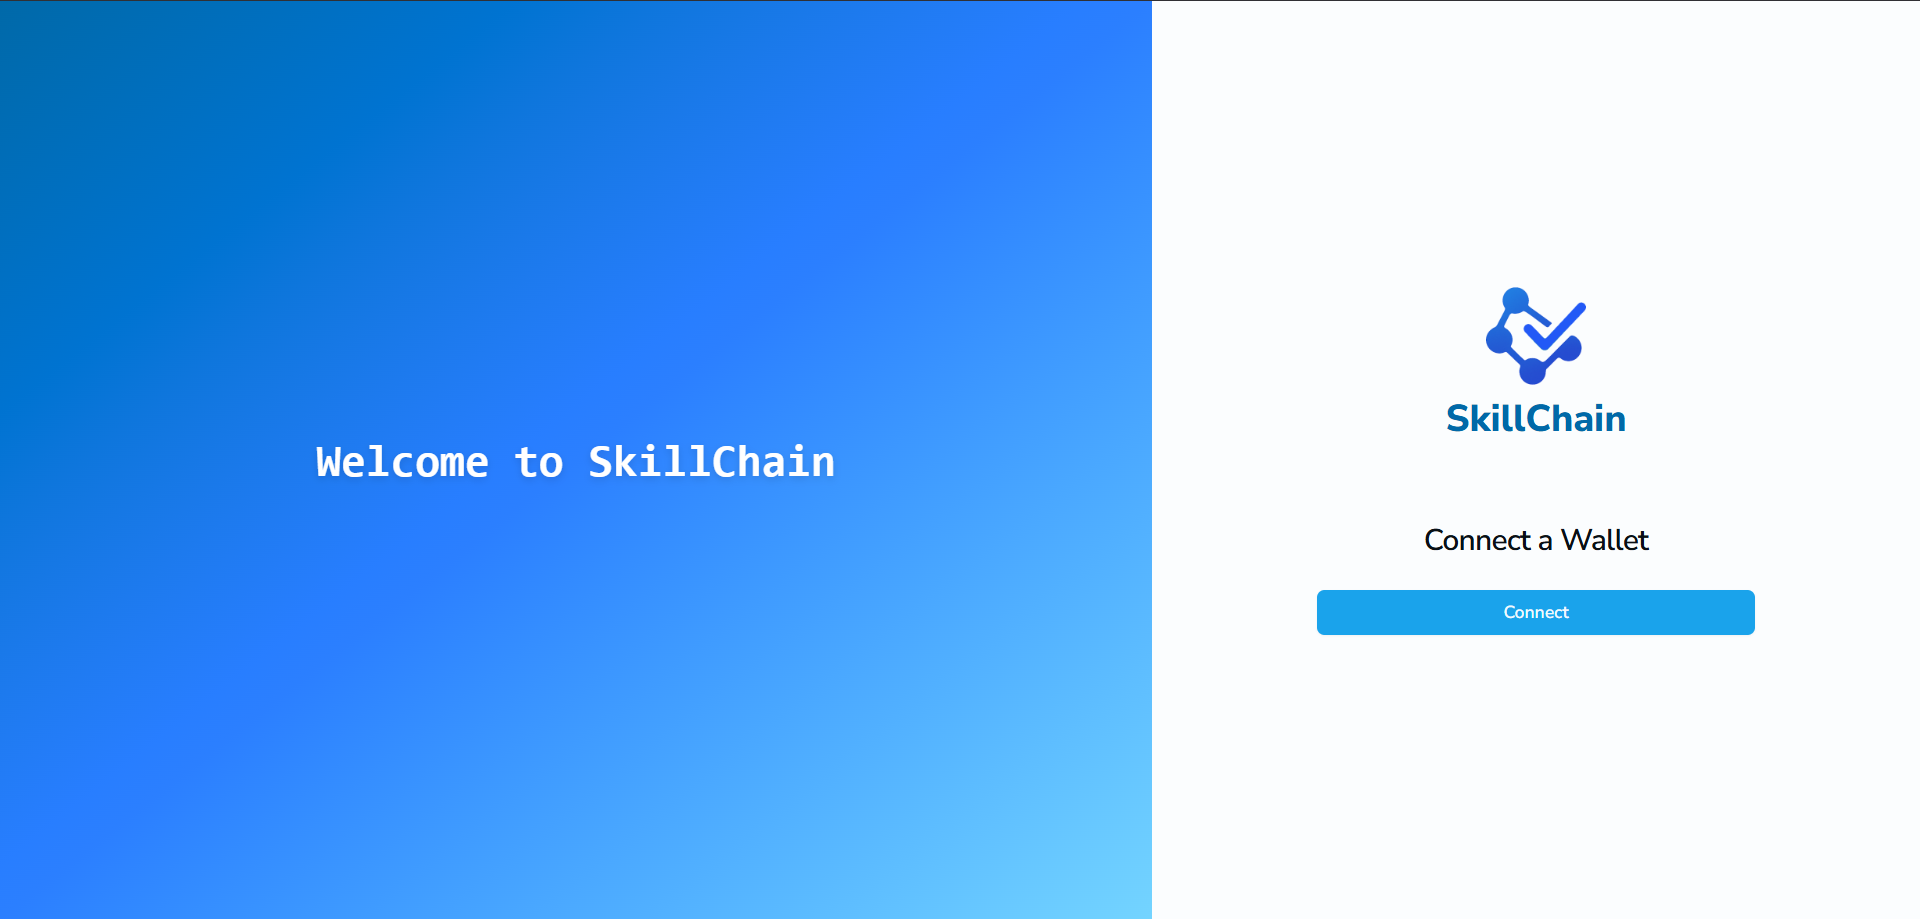
\includegraphics[width=0.99\textwidth, frame]{ui/login.png}
  \caption{Trang kết nối tài khoản}
  \label{fig:login-page}
\end{figure}

Tại trang này, người dùng có thể nhấn nút ``Connect'' để chọn ví muốn kết nối.

\begin{figure}[H]
  \centering
  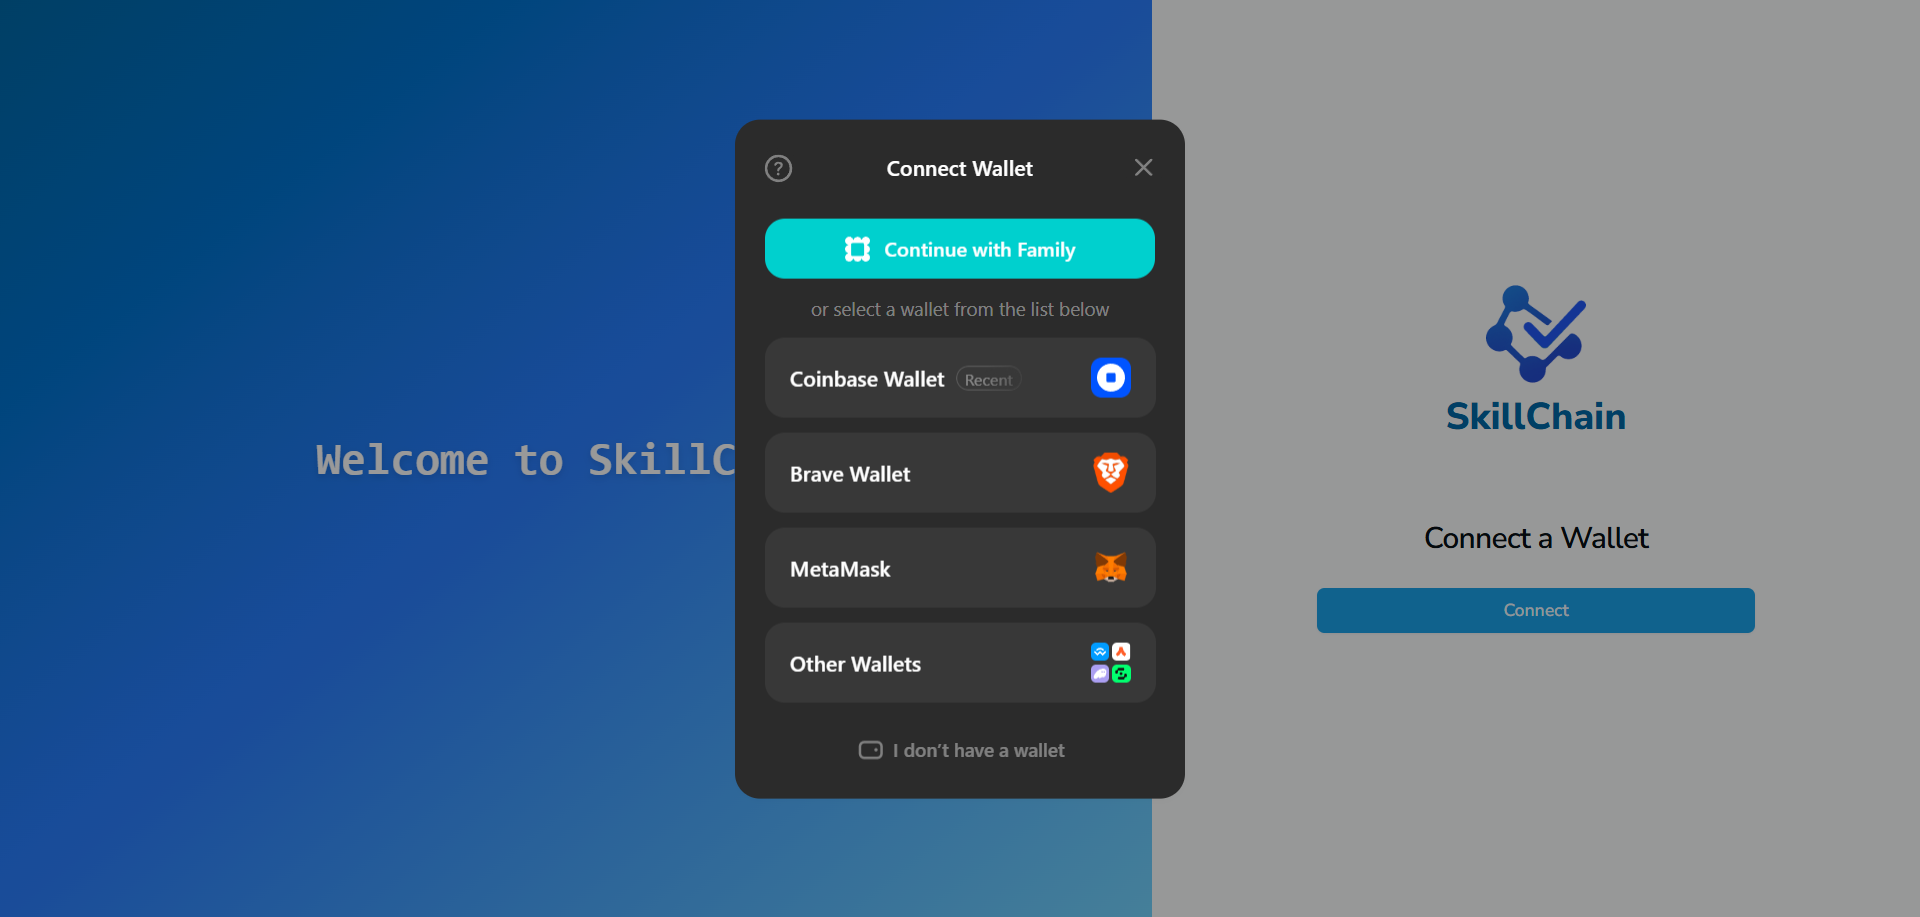
\includegraphics[width=0.99\textwidth, frame]{ui/login-wallets-page.png}
  \caption{Hộp thoại chọn ví kết nối}
  \label{fig:login-wallets-page}
\end{figure}

Sau khi kết nối thành công, hệ thống sẽ điều hướng người dùng đến trang chủ.

\begin{figure}[H]
  \centering
  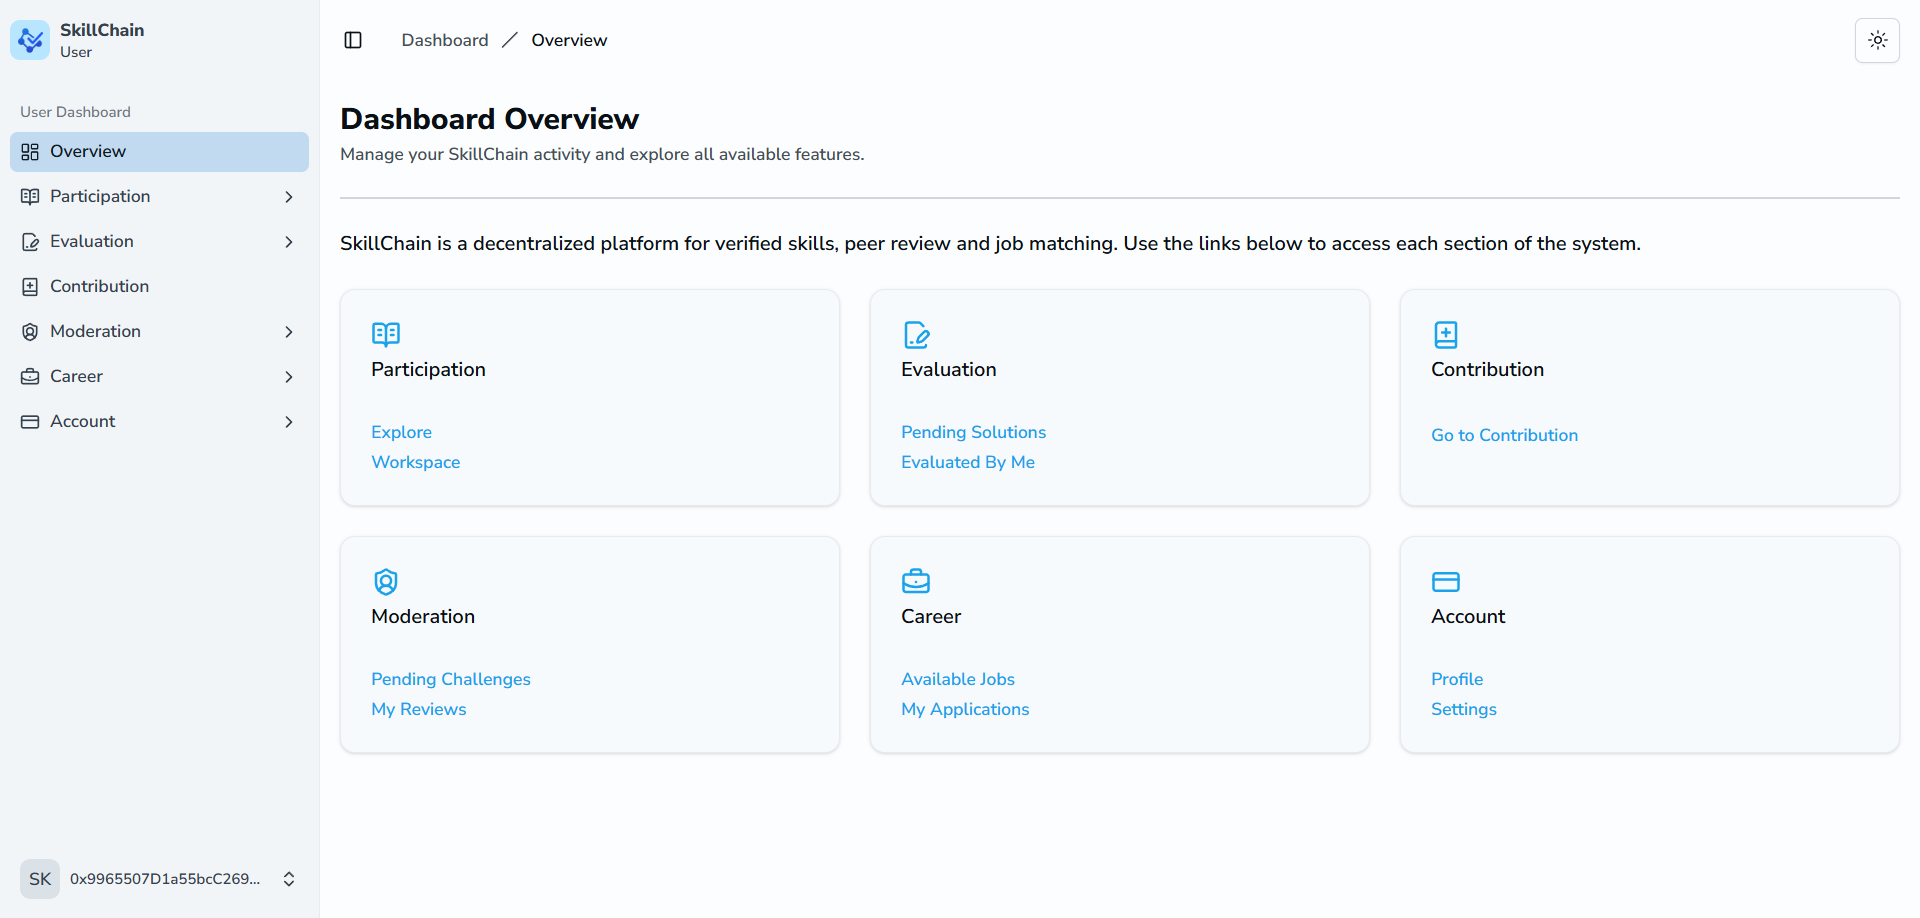
\includegraphics[width=0.99\textwidth, frame]{ui/home-page.png}
  \caption{Trang chủ}
  \label{fig:home-page}
\end{figure}

\subsection{Trang quản lý tài khoản}

\subsubsection{Trang thông tin cá nhân}

Để xem thông tin cá nhân, người dùng cần chọn \textbf{Account} $\rightarrow$ \textbf{Profile}.

\begin{figure}[H]
  \centering
  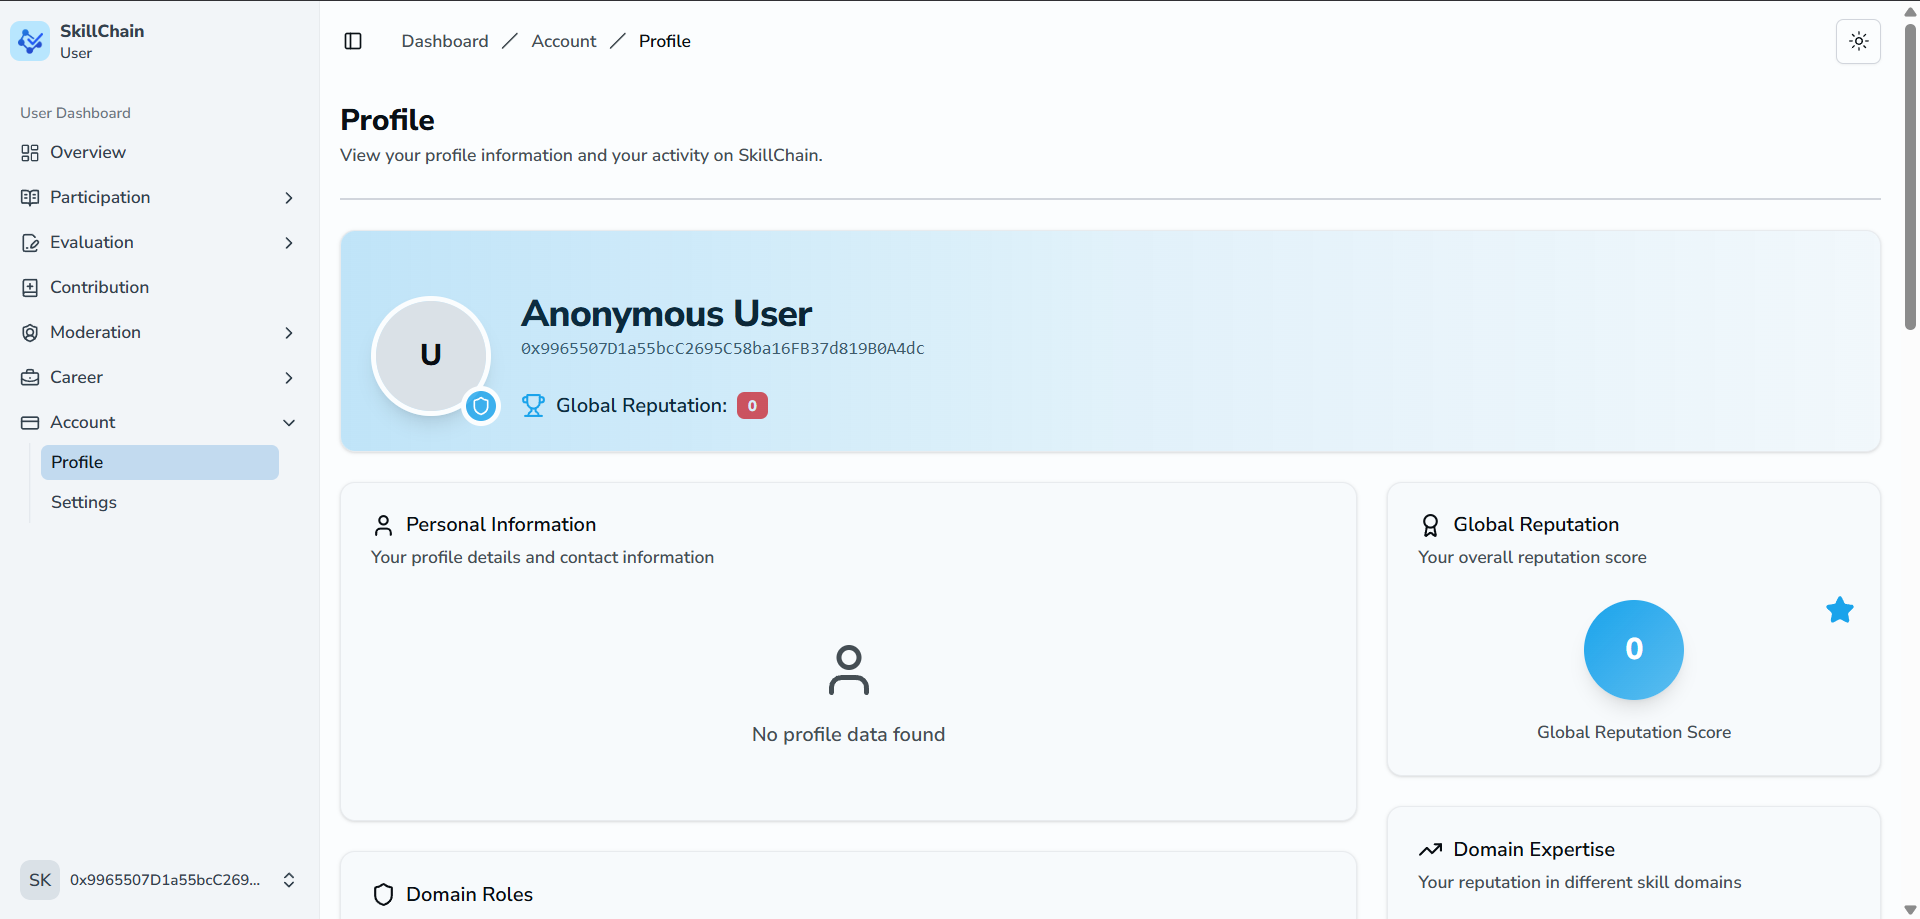
\includegraphics[width=0.99\textwidth, frame]{ui/unregistered-account-page.png}
  \caption{Trang thông tin tài khoản khi chưa đăng ký}
  \label{fig:unregistered-account-page}
\end{figure}

Ở góc dưới bên trái, hệ thống hiển thị quyền của người dùng đối với từng lĩnh vực chuyên môn, bao gồm khả năng đóng góp, kiểm duyệt và đánh giá.

\begin{figure}[H]
  \centering
  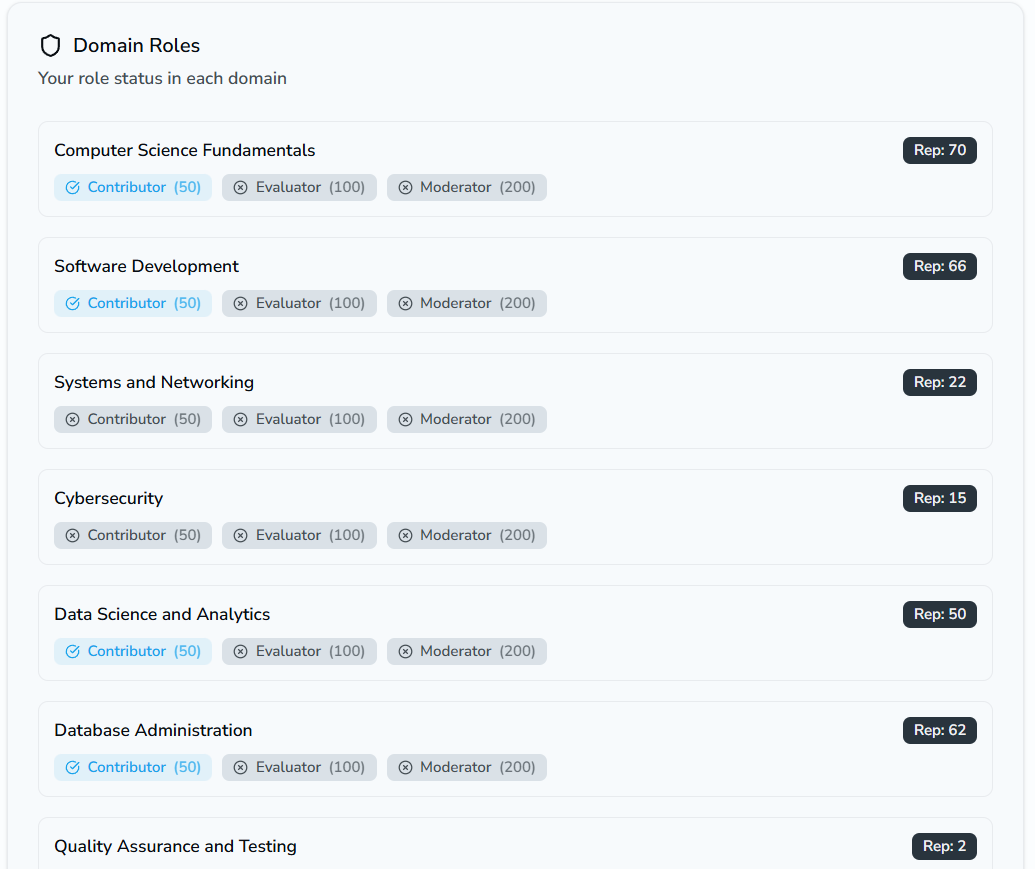
\includegraphics[width=0.99\textwidth, frame]{ui/domain-roles-page.png}
  \caption{Bảng vai trò của người dùng theo lĩnh vực chuyên môn}
  \label{fig:domain-roles-page}
\end{figure}

Hồ sơ uy tín được hiển thị ở góc dưới bên phải, bao gồm chỉ số uy tín toàn cục và uy tín theo từng lĩnh vực chuyên môn.

\begin{figure}[H]
  \centering
  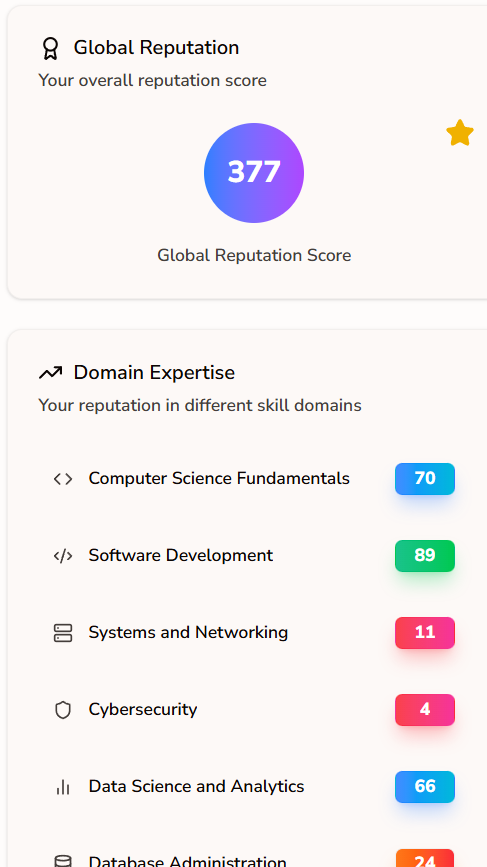
\includegraphics[width=0.5\textwidth, frame]{ui/reputation-profile.png}
  \caption{Hồ sơ uy tín}
  \label{fig:reputation-profile}
\end{figure}

\subsubsection{Trang cài đặt tài khoản}

Để chỉnh sửa thông tin cá nhân hoặc đăng ký tài khoản (nếu là lần kết nối đầu tiên), người dùng cần chọn \textbf{Account} $\rightarrow$ \textbf{Settings} và chuyển đến tab \textbf{Profile}.
Tại đây, người dùng có thể chọn ảnh đại diện, điền họ tên, địa chỉ email, nơi cư trú và tiểu sử để chỉnh sửa hoặc đăng ký thông tin cá nhân.  
Đối với lần đăng ký đầu tiên, hệ thống sẽ yêu cầu người dùng xác nhận giao dịch thông qua ví tiền điện tử để hoàn tất quá trình.

\begin{figure}[H]
  \centering
  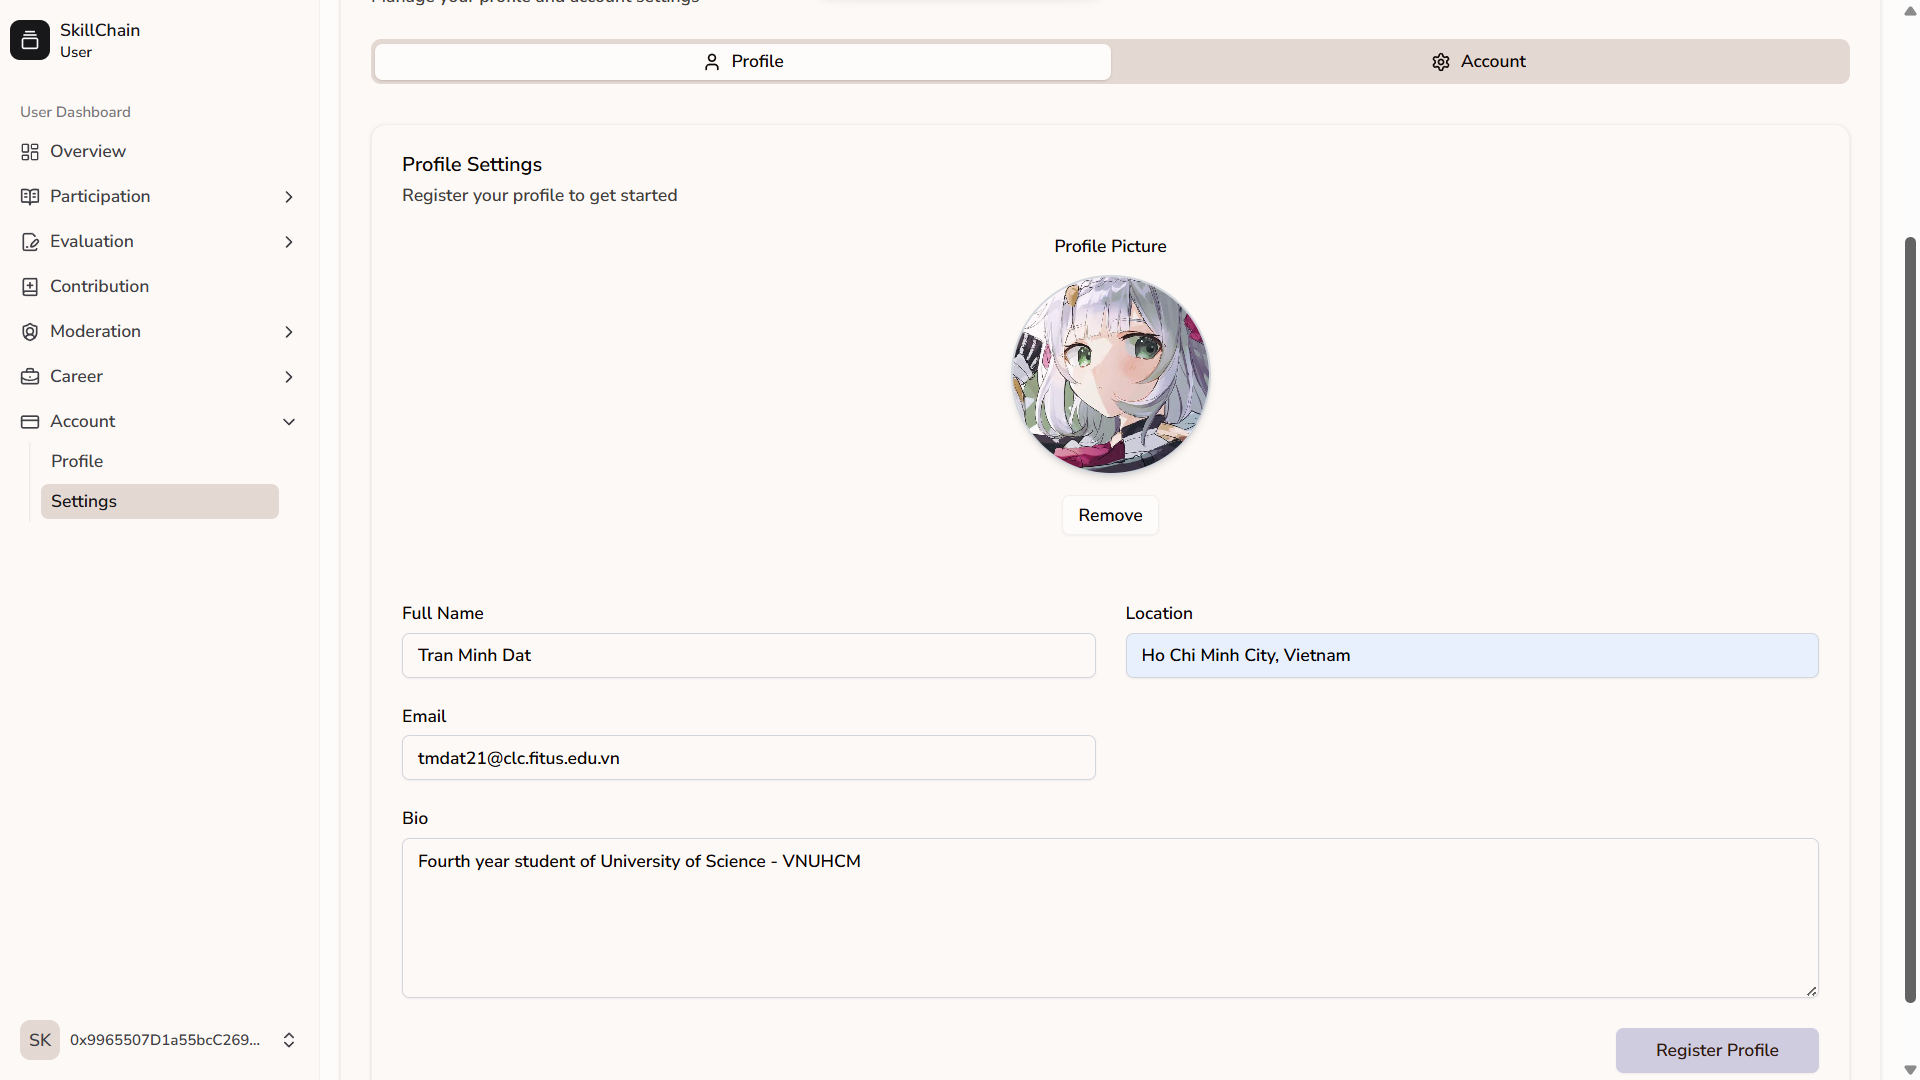
\includegraphics[width=0.99\textwidth, frame]{ui/register-account.png}
  \caption{Trang đăng ký thông tin cá nhân}
  \label{fig:register-account}
\end{figure}

\begin{figure}[H]
  \centering
  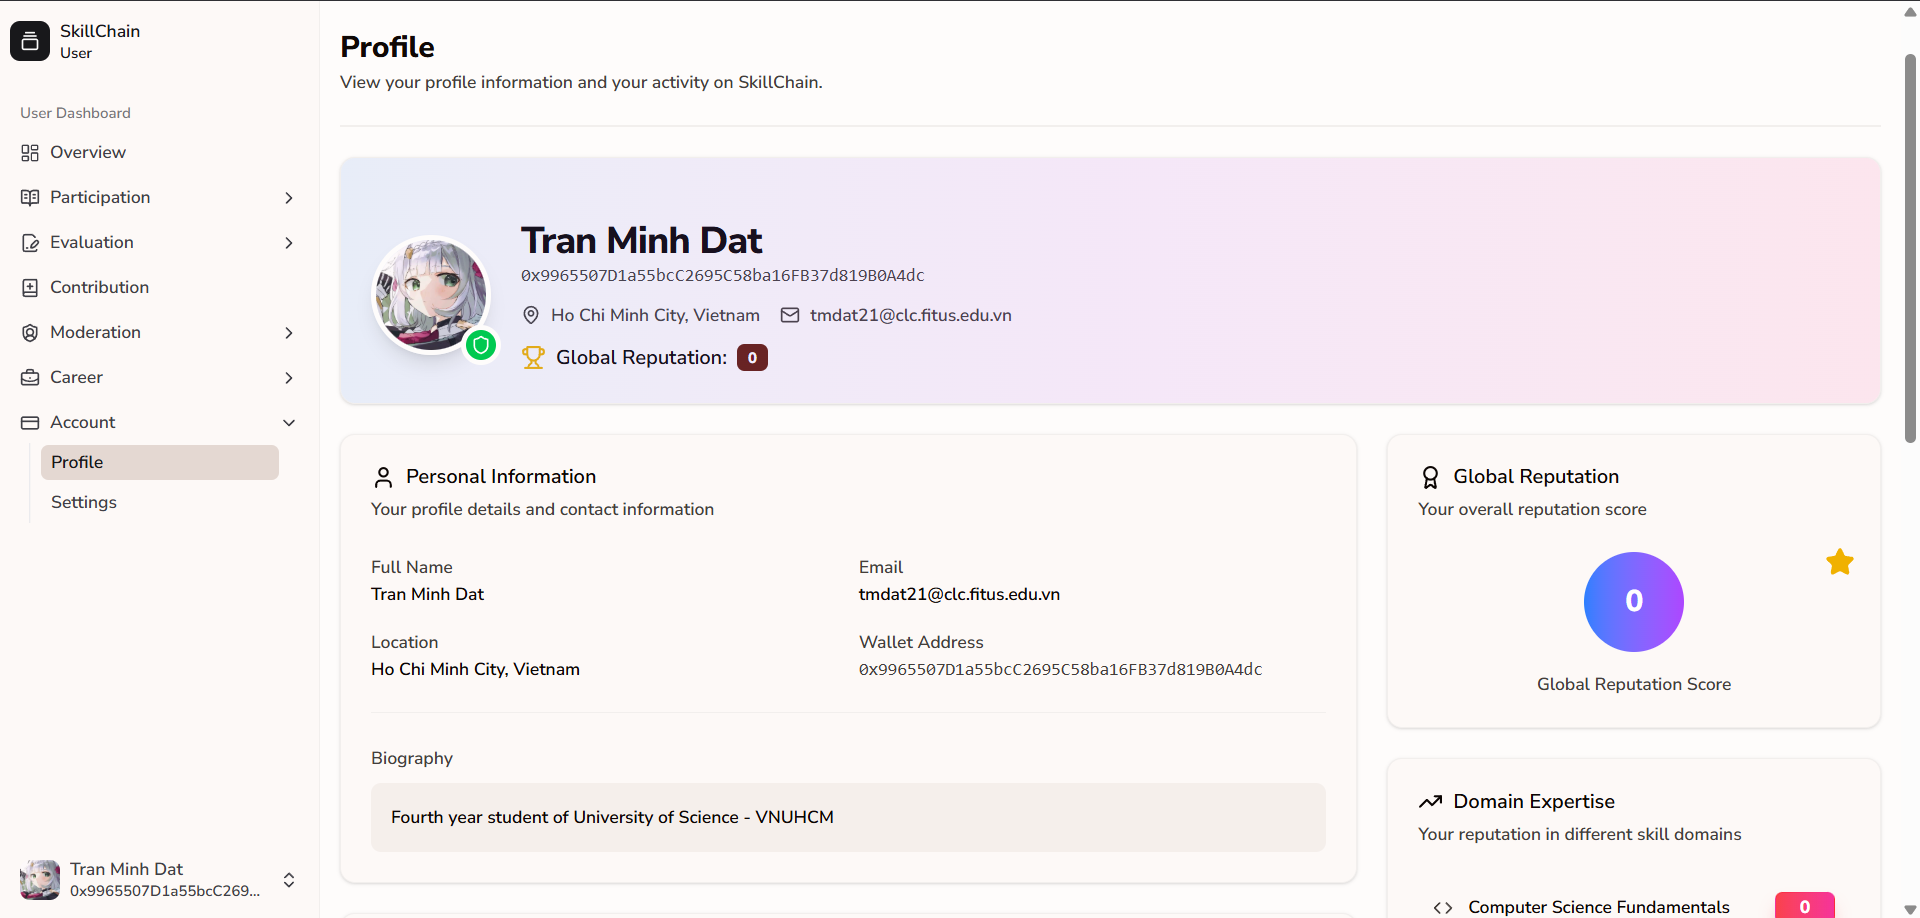
\includegraphics[width=0.99\textwidth, frame]{ui/registered-account-page.png}
  \caption{Trang thông tin cá nhân sau khi đã đăng ký}
  \label{fig:registered-account-page}
\end{figure}

Ngoài ra, người dùng cũng có thể truy cập tab \textbf{Account} để xem và cấu hình thông tin tài khoản liên quan đến hệ thống.

\begin{figure}[H]
  \centering
  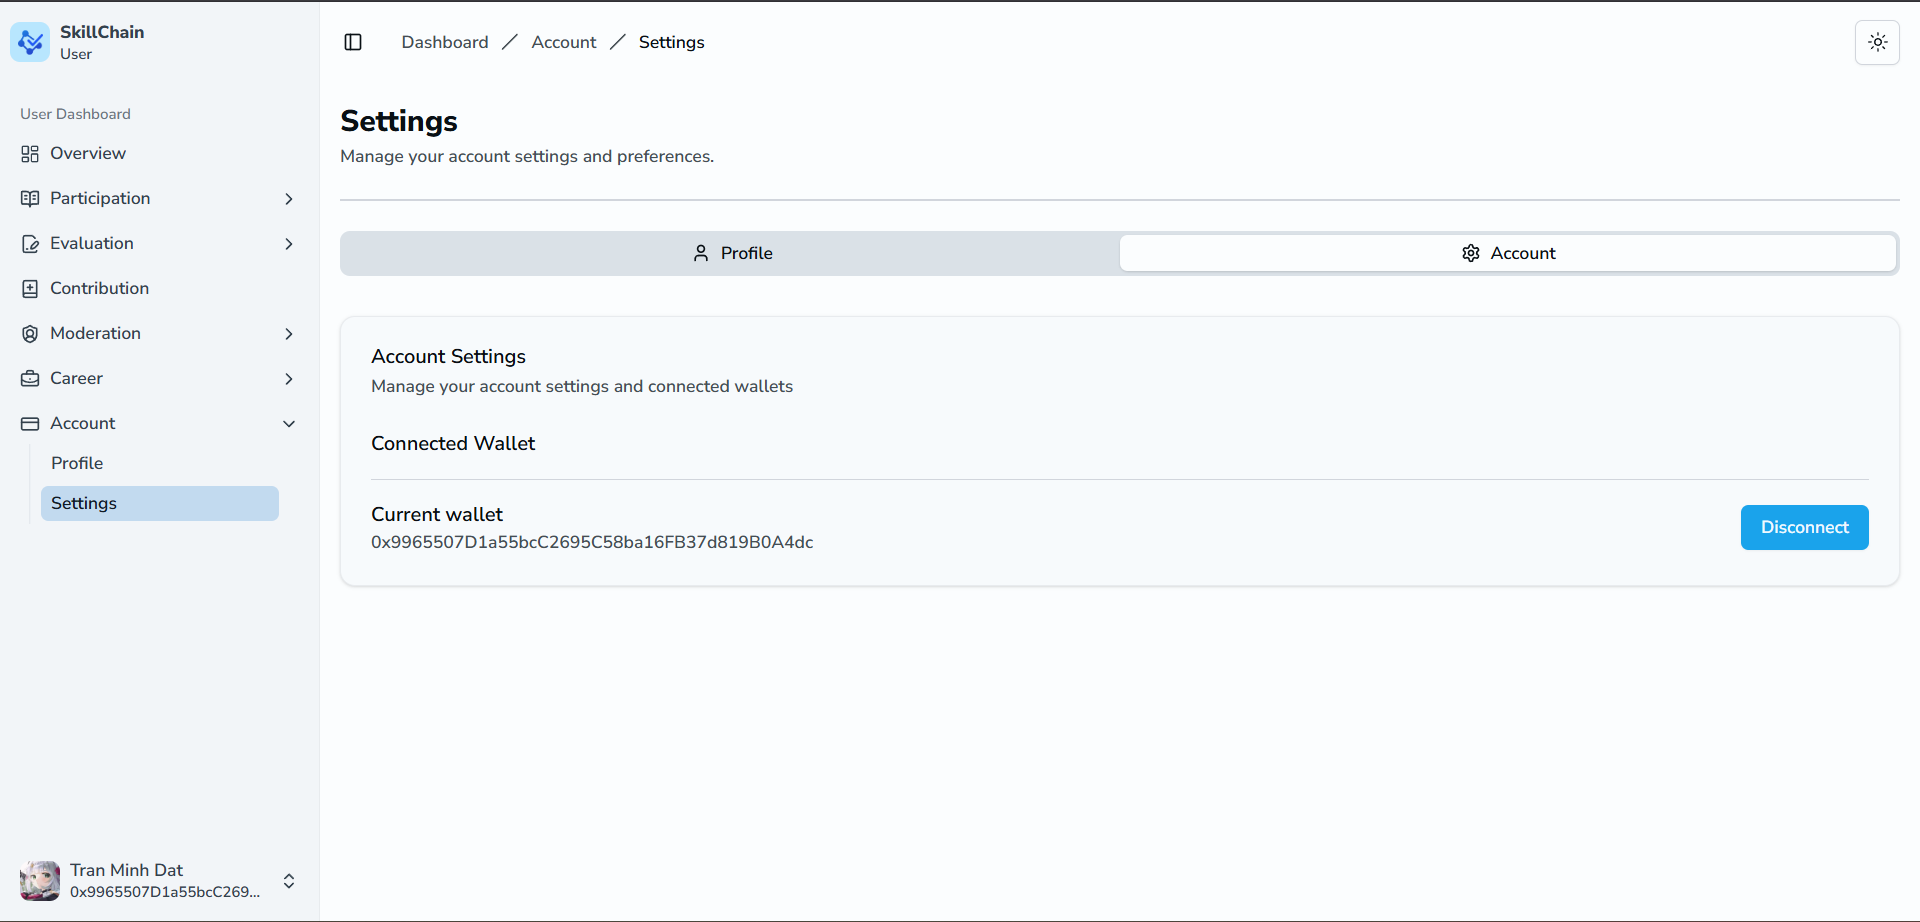
\includegraphics[width=0.99\textwidth, frame]{ui/account-settings-page.png}
  \caption{Trang thiết lập tài khoản}
  \label{fig:account-settings-page}
\end{figure}

\subsection{Trang đóng góp thử thách}

Để khởi tạo, quản lý và theo dõi các thử thách, người dùng cần truy cập tab \textbf{Contribution}.

\begin{figure}[H]
  \centering
  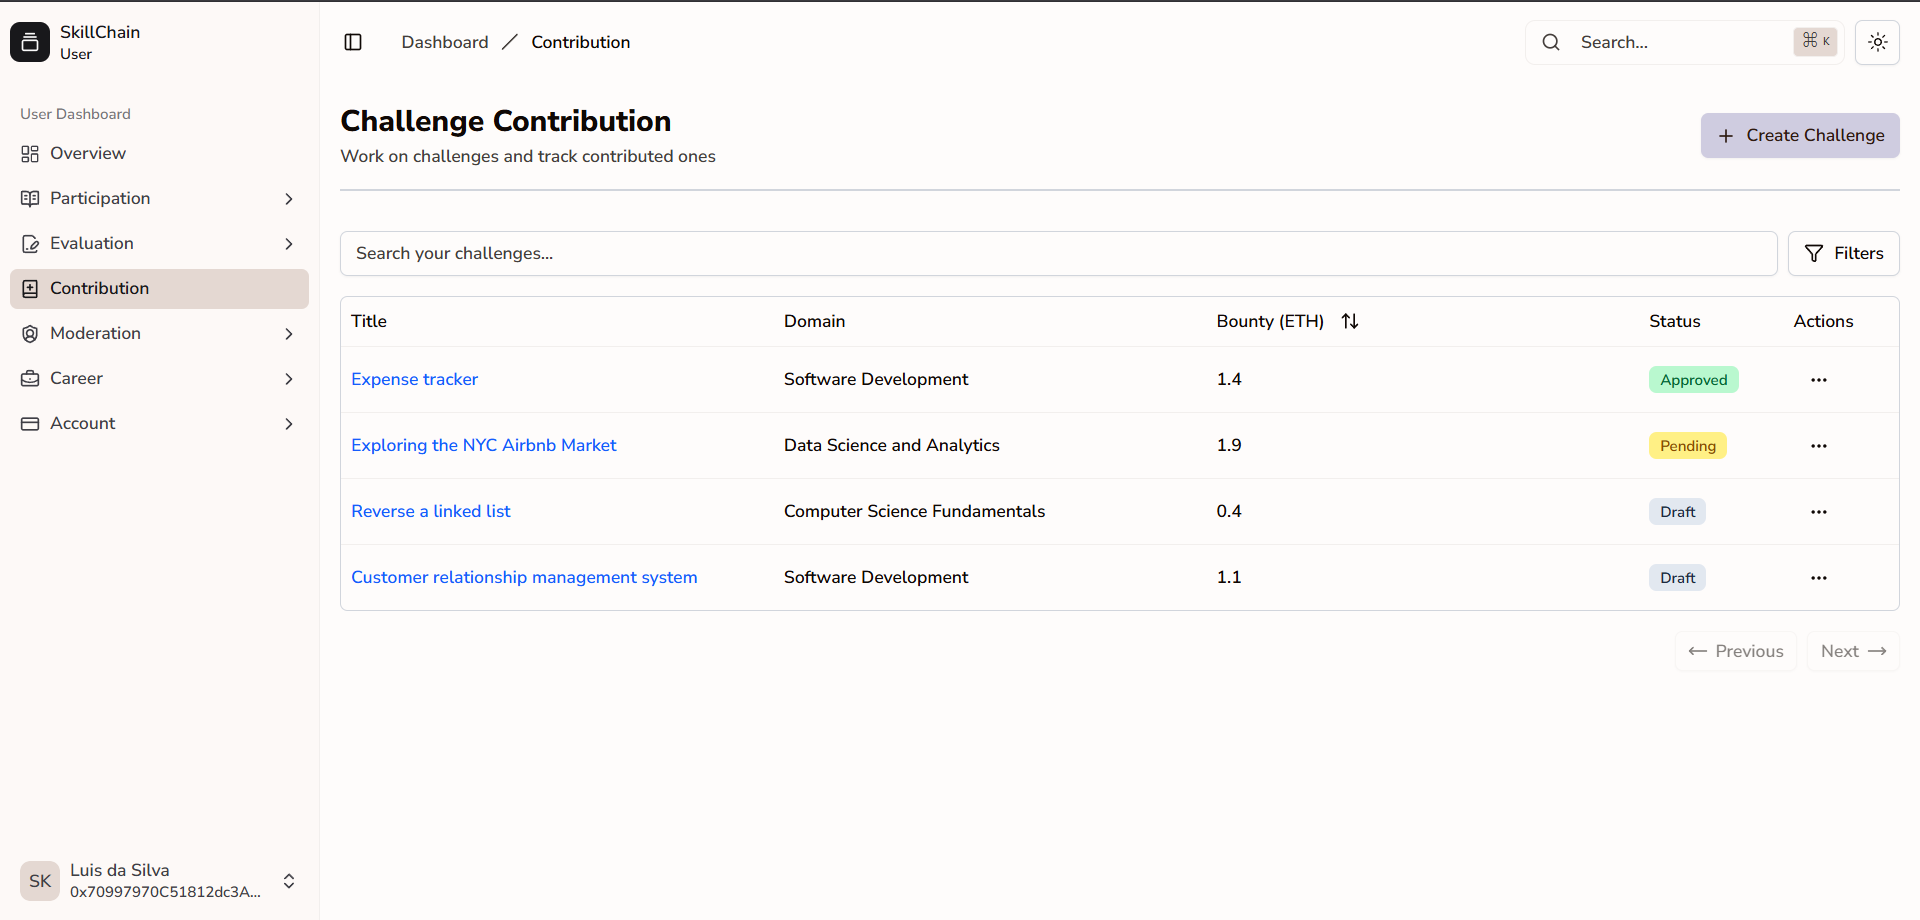
\includegraphics[width=0.99\textwidth, frame]{ui/contribution-page.png}
  \caption{Trang đóng góp thử thách}
  \label{fig:contribution-page}
\end{figure}

Tại đây, người dùng có thể xem danh sách các thử thách đã đóng góp, cùng với thông tin về loại thử thách, trạng thái và mức treo thưởng.  
Người dùng có thể xem chi tiết một thử thách bằng cách nhấn vào liên kết tên thử thách hoặc chọn ``View challenge'' từ nút ``Actions``.

\subsubsection{Tạo thử thách mới}

Để tạo một thử thách mới, người dùng nhấn nút ``Create Challenge'' ở góc trên bên phải.

\begin{figure}[H]
  \centering
  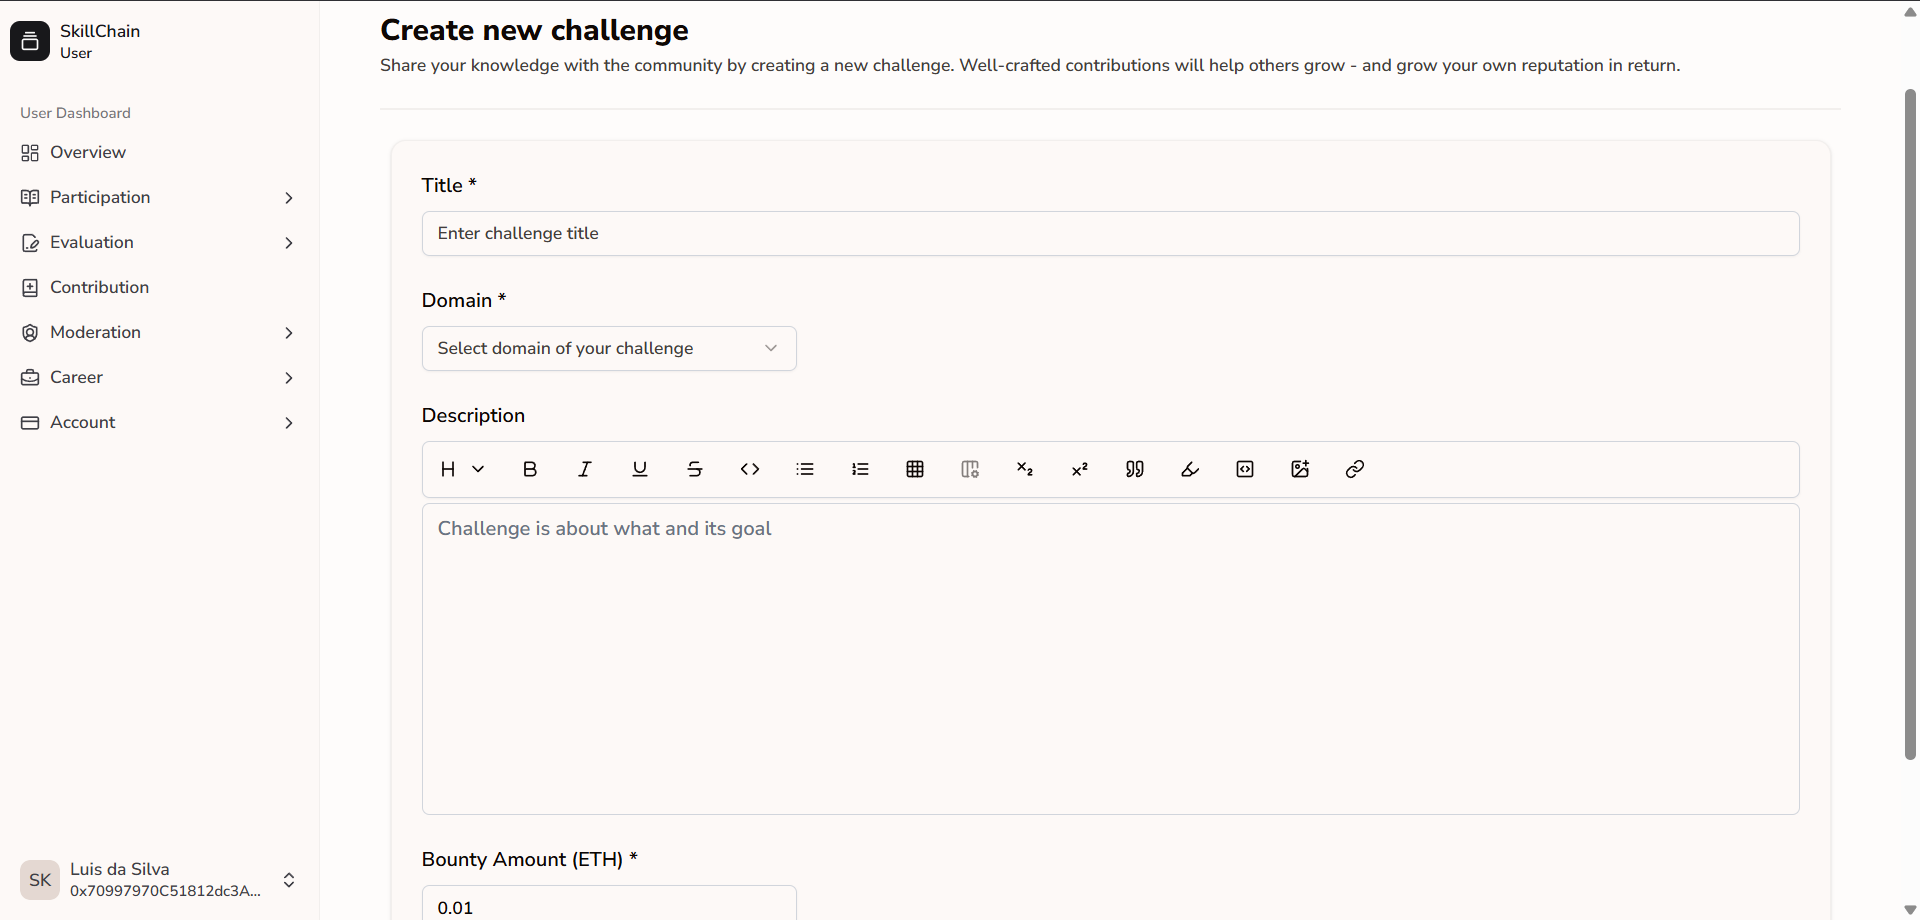
\includegraphics[width=0.99\textwidth, frame]{ui/create-challenge-page.png}
  \caption{Trang tạo thử thách mới}
  \label{fig:create-challenge-page}
\end{figure}

Tại trang này, người dùng nhập các thông tin quan trọng của thử thách, sau đó nhấn nút ``Create challenge''.  
Hệ thống sẽ yêu cầu xác thực giao dịch thông qua ví tiền điện tử để chính thức tạo thử thách ở trạng thái nháp.
Nếu người dùng không đủ chỉ số uy tín chuyên môn tương ứng với loại thử thách đang tạo, hệ thống sẽ hiển thị thông báo lỗi và không cho phép tạo thử thách.

\subsubsection{Chỉnh sửa thử thách}

Để chỉnh sửa một thử thách đang ở trạng thái nháp, người dùng cần truy cập trang chi tiết của thử thách và nhấn nút ``Edit''.

\begin{figure}[H]
  \centering
  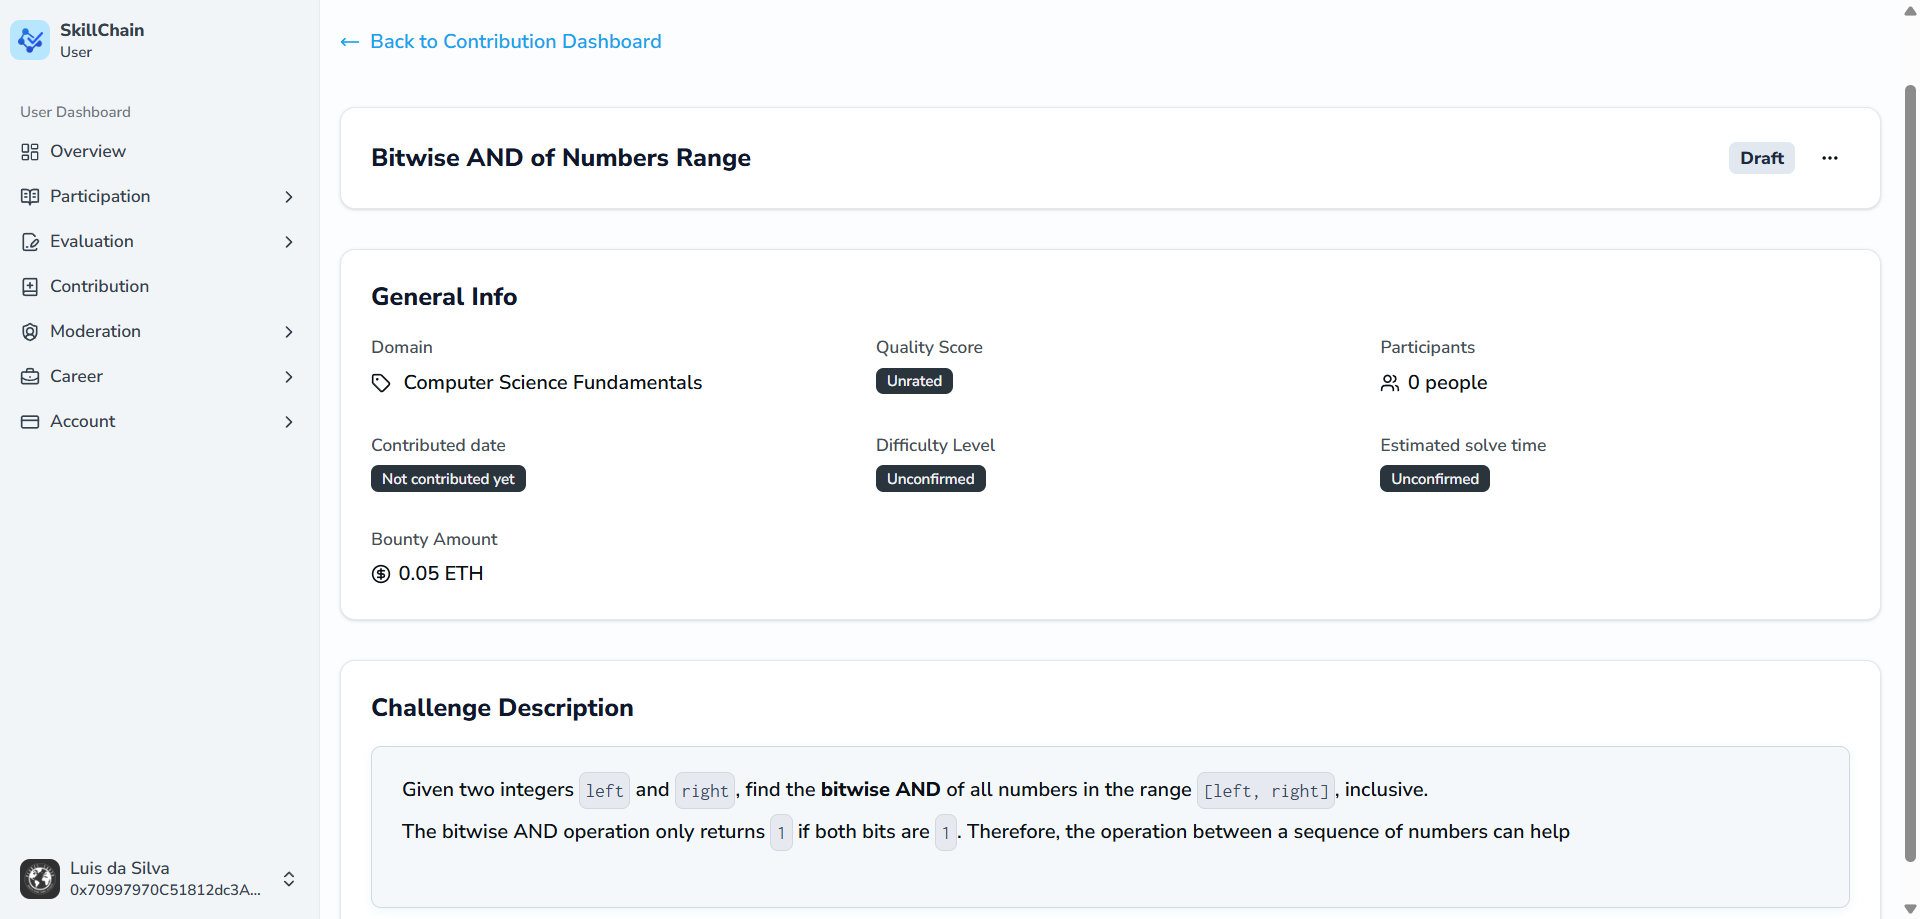
\includegraphics[width=0.99\textwidth, frame]{ui/contribution-challenge-detail-page.png}
  \caption{Trang chi tiết thử thách đã tạo}
  \label{fig:contribution-challenge-detail-page}
\end{figure}

\begin{figure}[H]
  \centering
  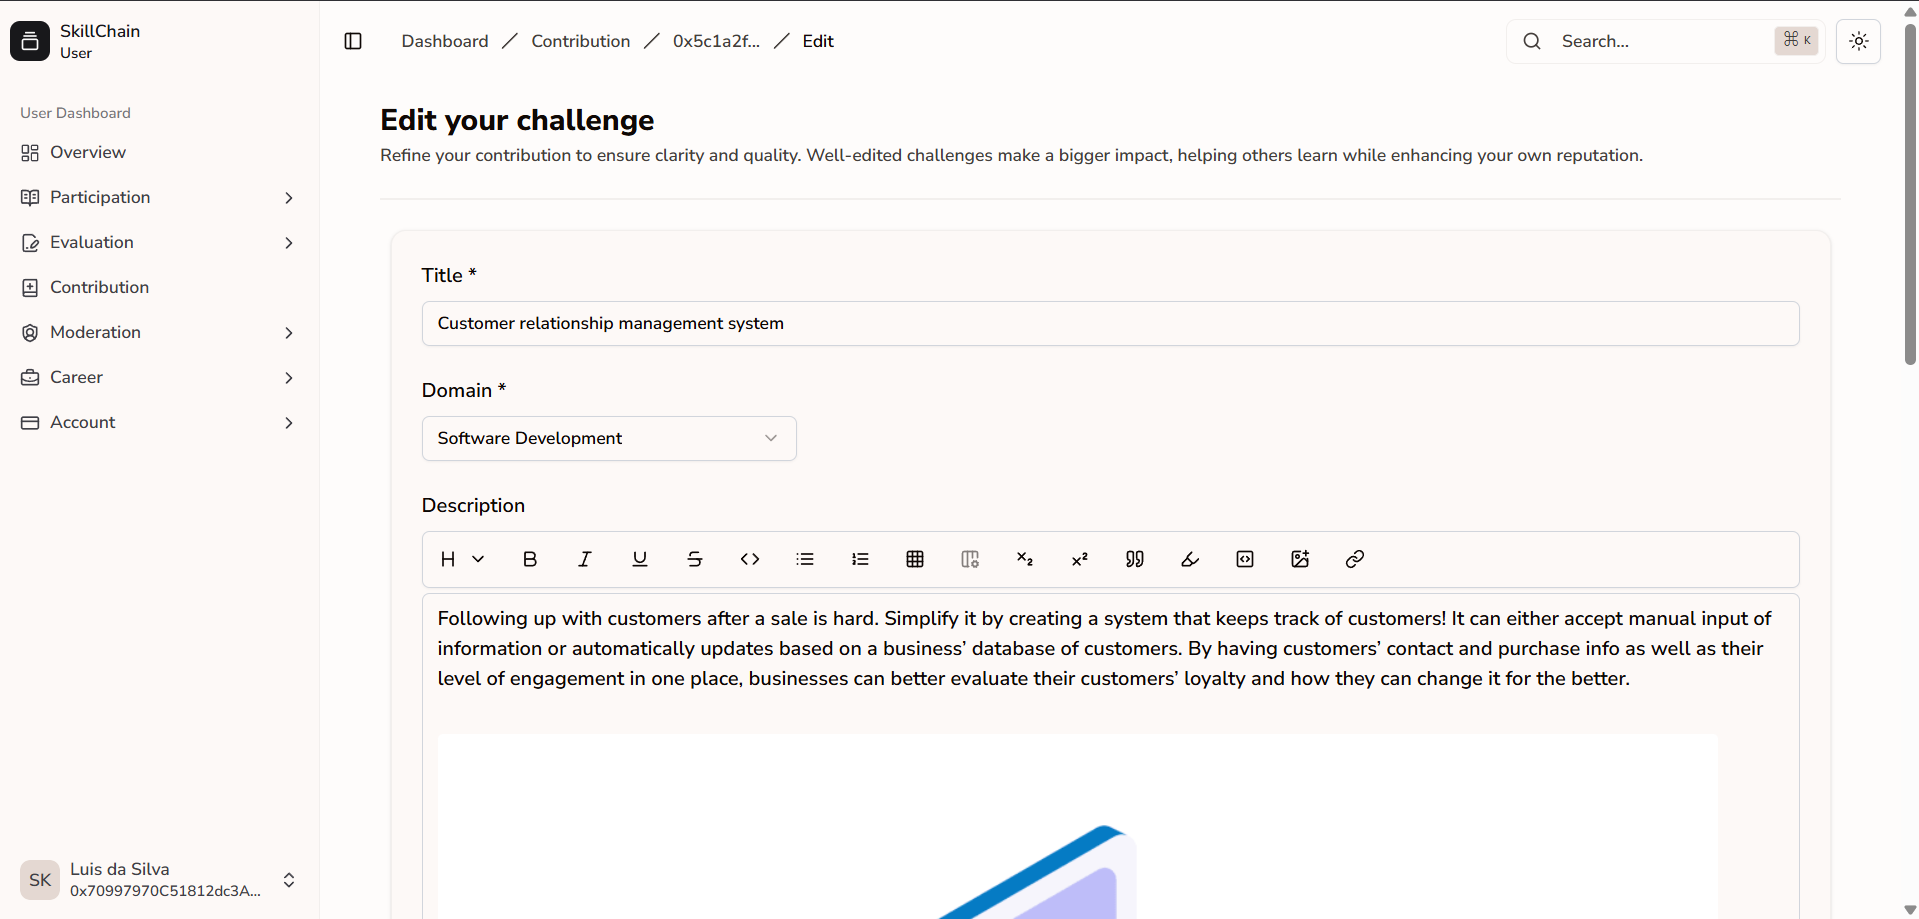
\includegraphics[width=0.99\textwidth, frame]{ui/contribution-challenge-edit-page.png}
  \caption{Trang chỉnh sửa thử thách}
  \label{fig:contribution-challenge-edit-page}
\end{figure}

Người dùng có thể chỉnh sửa nội dung thử thách tại đây và nhấn ``Save changes'' để lưu thay đổi.

\subsubsection{Gửi thử thách cho kiểm duyệt}

Để gửi thử thách đến bên kiểm duyệt, người dùng truy cập trang chi tiết của thử thách và nhấn nút ``Contribute''.  
Hệ thống sẽ yêu cầu xác thực giao dịch thông qua ví tiền điện tử để chính thức chuyển thử thách sang trạng thái chờ kiểm duyệt.  
Sau khi gửi đi, thử thách sẽ bị khóa và không còn có thể chỉnh sửa được nữa.

\subsection{Trang kiểm duyệt thử thách}

\subsubsection{Xem thử thách chờ kiểm duyệt}

Để xem danh sách các thử thách đang chờ kiểm duyệt, người dùng truy cập \textbf{Moderation} $\rightarrow$ \textbf{Pending Challenge}.  
Tại đây, người dùng có thể xem thông tin chi tiết từng thử thách, bao gồm số lượng người đã tham gia kiểm duyệt.

\begin{figure}[H]
  \centering
  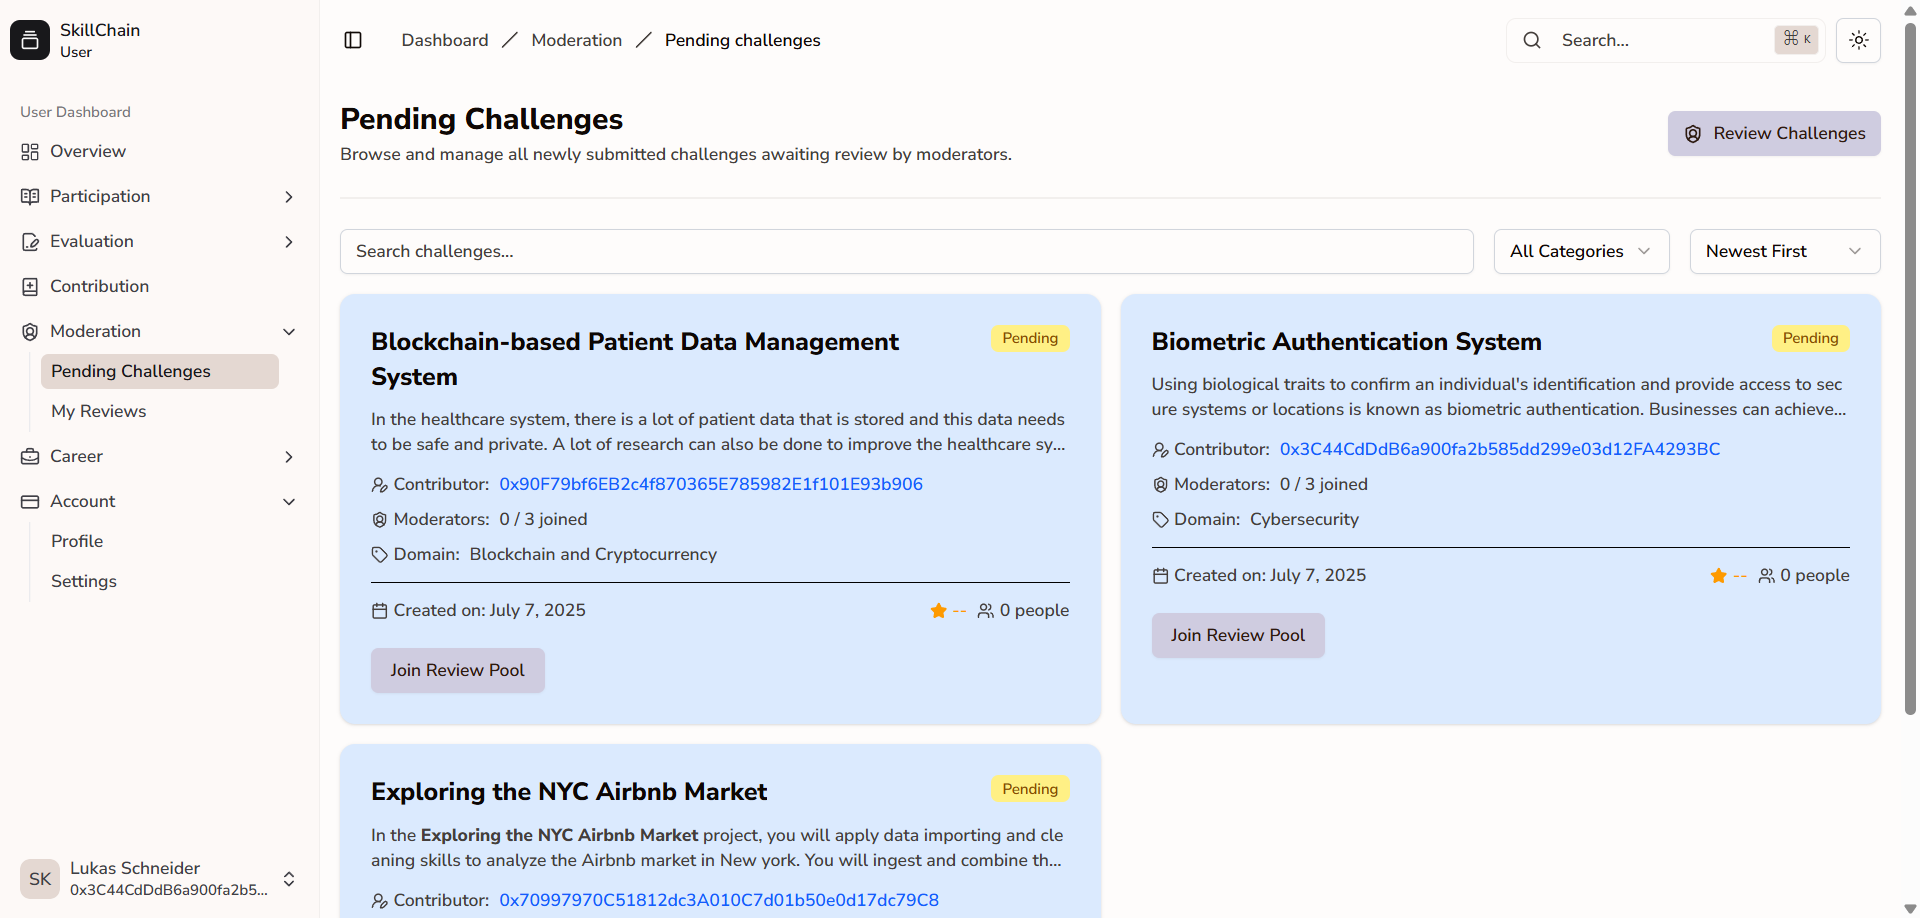
\includegraphics[width=0.99\textwidth, frame]{ui/moderation-pending-challenges-page.png}
  \caption{Trang danh sách thử thách chờ kiểm duyệt}
  \label{fig:moderation-pending-challenges-page}
\end{figure}

\subsubsection{Tham gia kiểm duyệt thử thách}

Để tham gia kiểm duyệt một thử thách, người dùng nhấn nút ``Join Review Pool'' tại thử thách mong muốn.  
Hệ thống sẽ yêu cầu xác thực giao dịch thông qua ví tiền điện tử để hoàn tất việc tham gia kiểm duyệt.
Nếu người dùng không đủ chỉ số uy tín chuyên môn tương ứng với loại thử thách, hệ thống sẽ hiển thị thông báo lỗi và không cho phép tham gia.

\subsubsection{Thực hiện kiểm duyệt}

Để bắt đầu kiểm duyệt, người dùng truy cập \textbf{Moderation} $\rightarrow$ \textbf{My Reviews} để xem danh sách các thử thách mà mình đã tham gia kiểm duyệt.  
Sau đó, chọn thử thách tương ứng và nhấn nút ``Edit review''.

\begin{figure}[H]
  \centering
  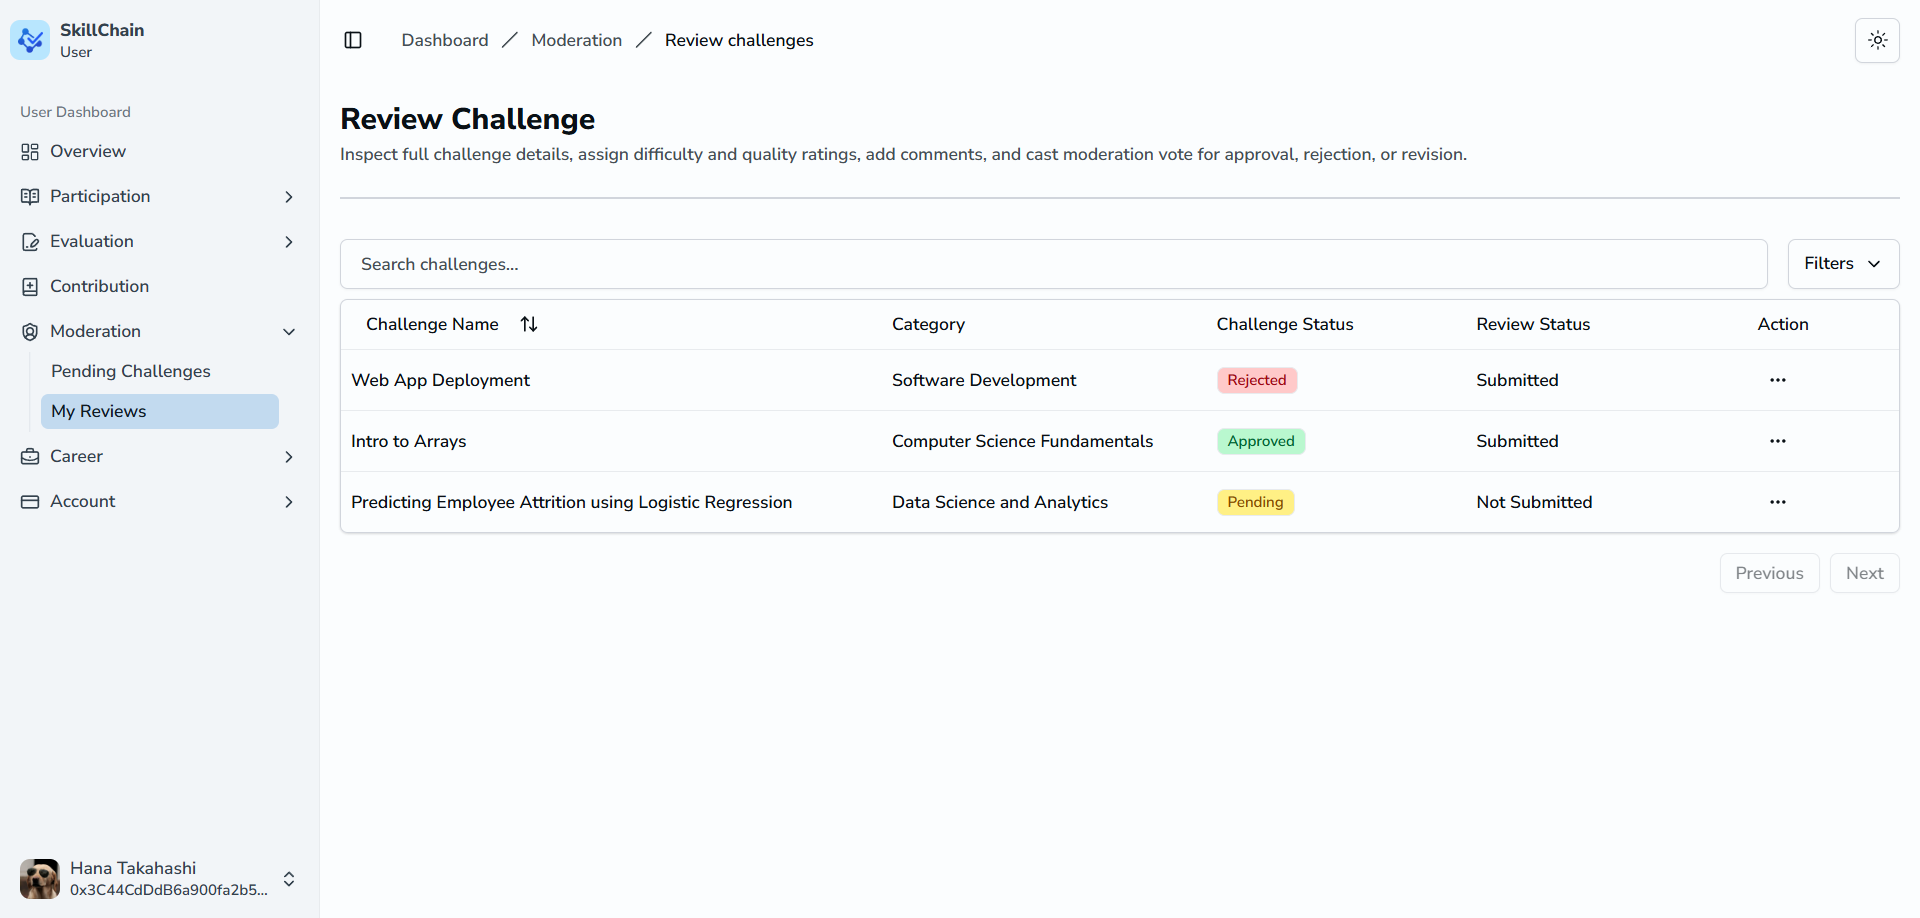
\includegraphics[width=0.99\textwidth, frame]{ui/moderation-my-reviews-page.png}
  \caption{Trang danh sách thử thách đã và đang kiểm duyệt}
  \label{fig:moderation-my-reviews-page}
\end{figure}

Tại trang này, người dùng có thể xem chi tiết phiên kiểm duyệt.  
Để thực hiện đánh giá, chuyển sang tab \textbf{Review Form}.

Trong biểu mẫu kiểm duyệt, người dùng cần:
\begin{itemize}
  \item Chọn \textbf{Yes/No} cho từng tiêu chí đánh giá chất lượng.
  \item Đề xuất độ khó và thời gian giải ước tính.
  \item Có thể lưu tạm nội dung đánh giá hoặc gửi luôn.
\end{itemize}

Sau khi hoàn tất, nhấn nút ``Submit Review'' để nộp đánh giá.  
Giao dịch sẽ cần được xác thực qua ví tiền điện tử, và sau khi gửi, nội dung đánh giá sẽ không thể chỉnh sửa.

\begin{figure}[H]
  \centering
  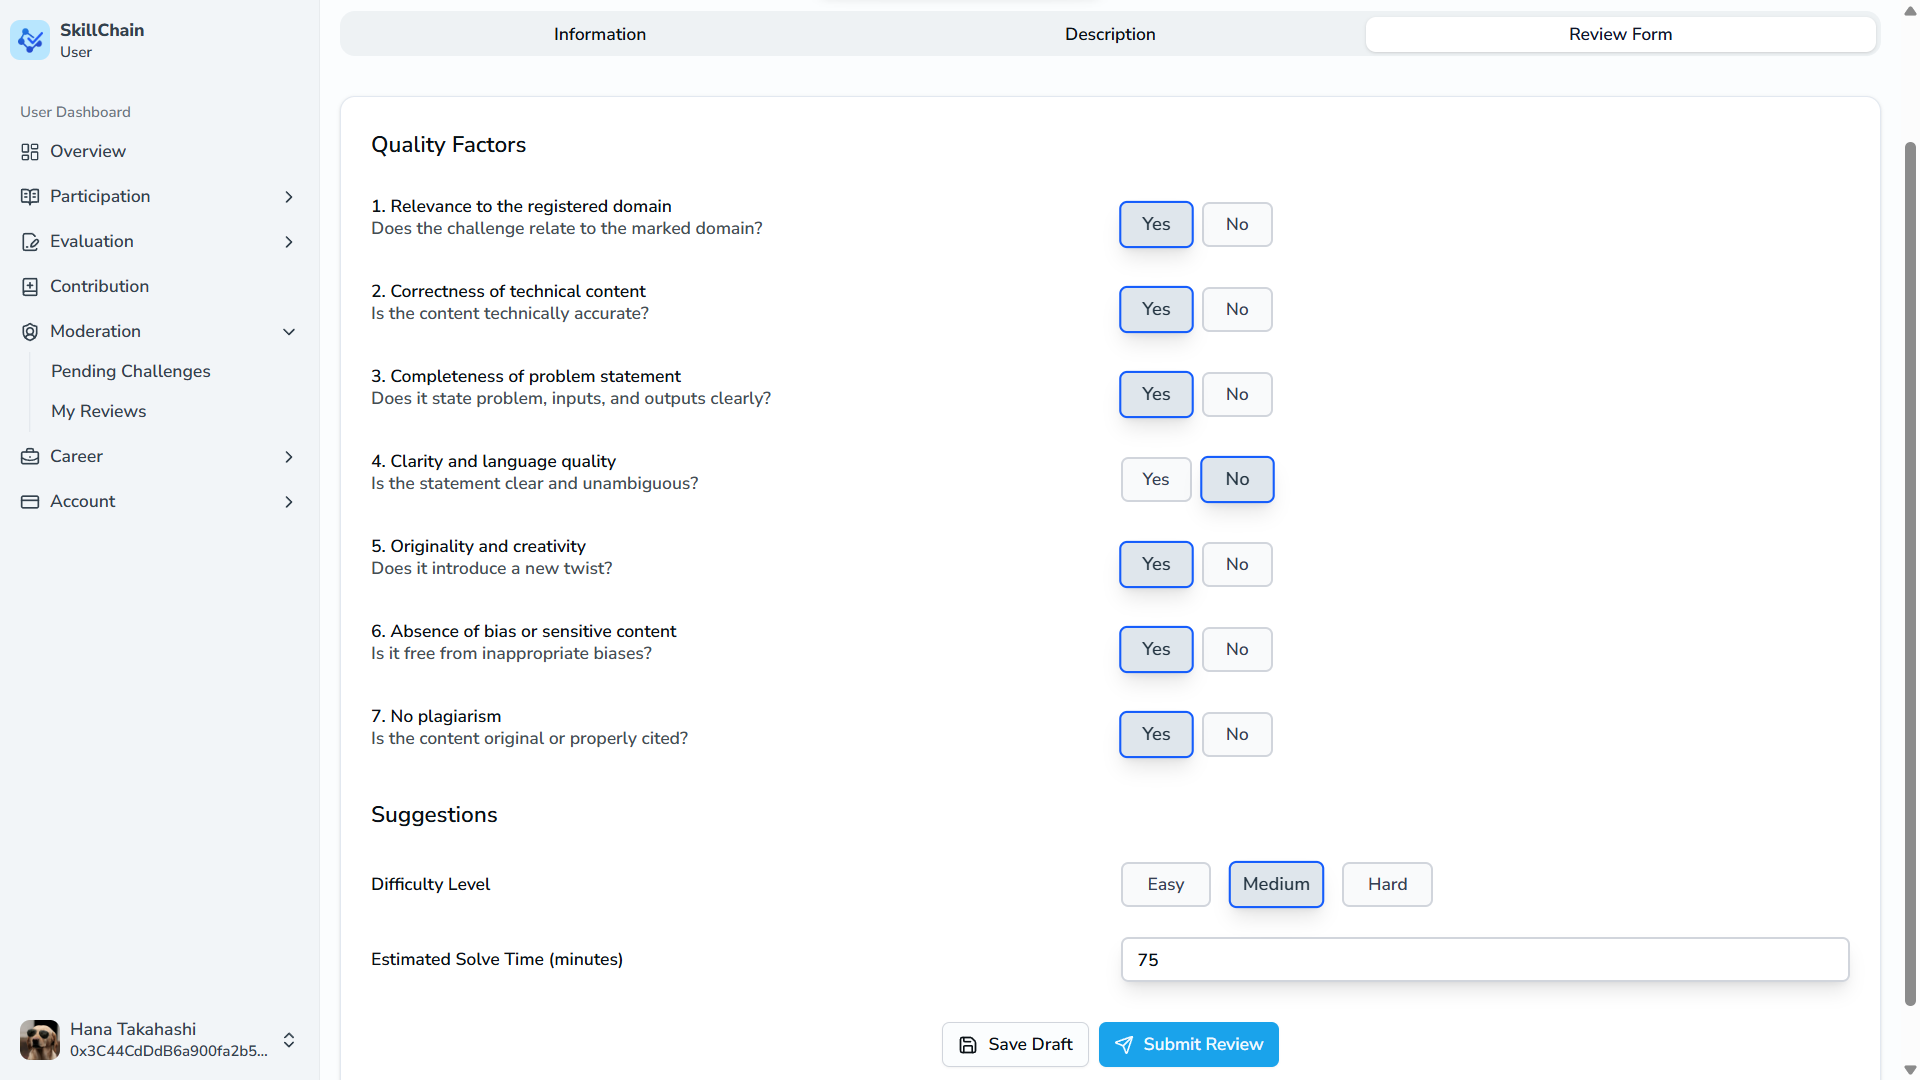
\includegraphics[width=0.99\textwidth, frame]{ui/moderation-review-form.png}
  \caption{Biểu mẫu kiểm duyệt chất lượng thử thách}
  \label{fig:moderation-review-form}
\end{figure}

\subsubsection{Xem thông tin phiên kiểm duyệt}

Khi phiên kiểm duyệt kết thúc, thông tin chi tiết về phiên sẽ được hiển thị cho người đóng góp và các kiểm duyệt viên.  
Thông tin này bao gồm danh sách người kiểm duyệt, số điểm đánh giá, và phần token thưởng tương ứng.

\begin{figure}[H]
  \centering
  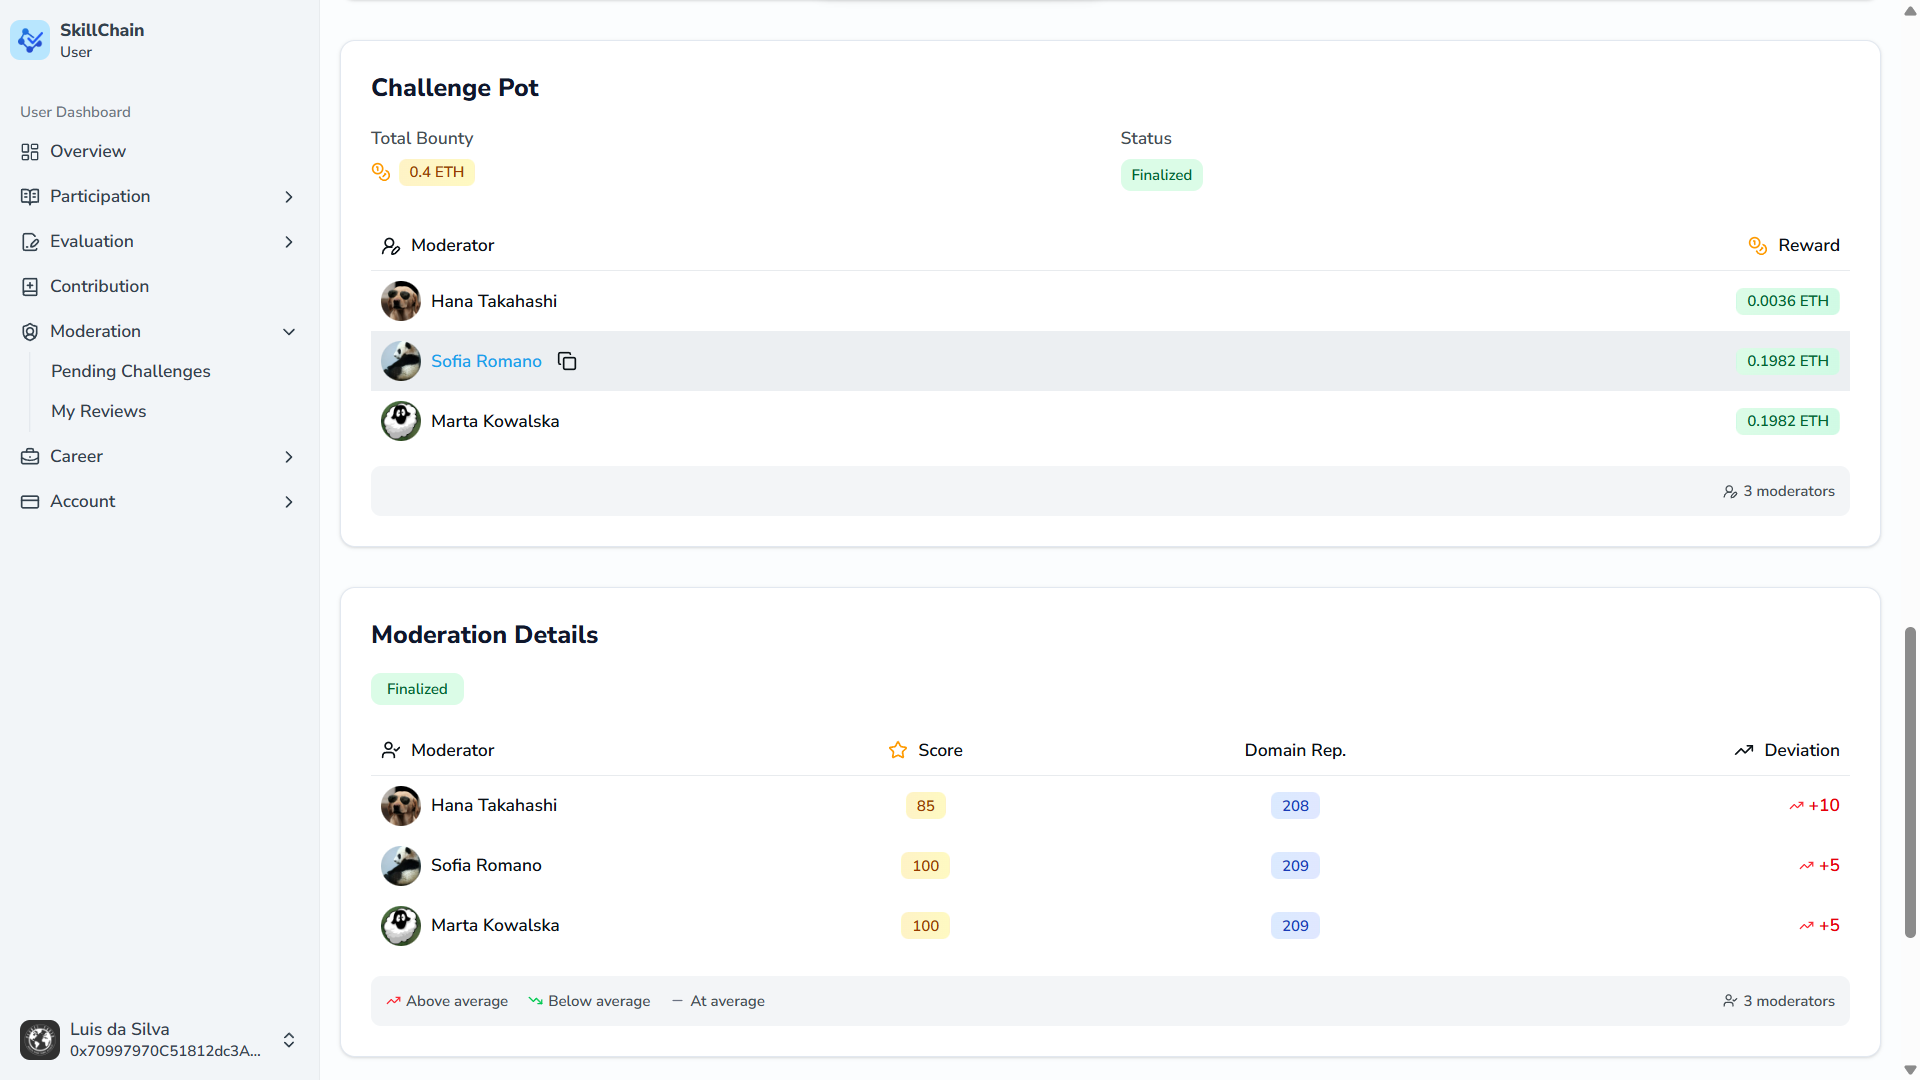
\includegraphics[width=0.99\textwidth, frame]{ui/challenge-moderation-pot-info.png}
  \caption{Thông tin chi tiết của một phiên kiểm duyệt}
  \label{fig:challenge-moderation-pot-info}
\end{figure}

\subsection{Trang tham gia thử thách}

\subsubsection{Xem thử thách đang hiện hành}

Để xem danh sách các thử thách đang mở, người dùng truy cập \textbf{Participation} $\rightarrow$ \textbf{Explore}.  
Tại đây, người dùng có thể xem chi tiết nội dung từng thử thách bằng cách nhấn vào thẻ tương ứng.

\begin{figure}[H]
  \centering
  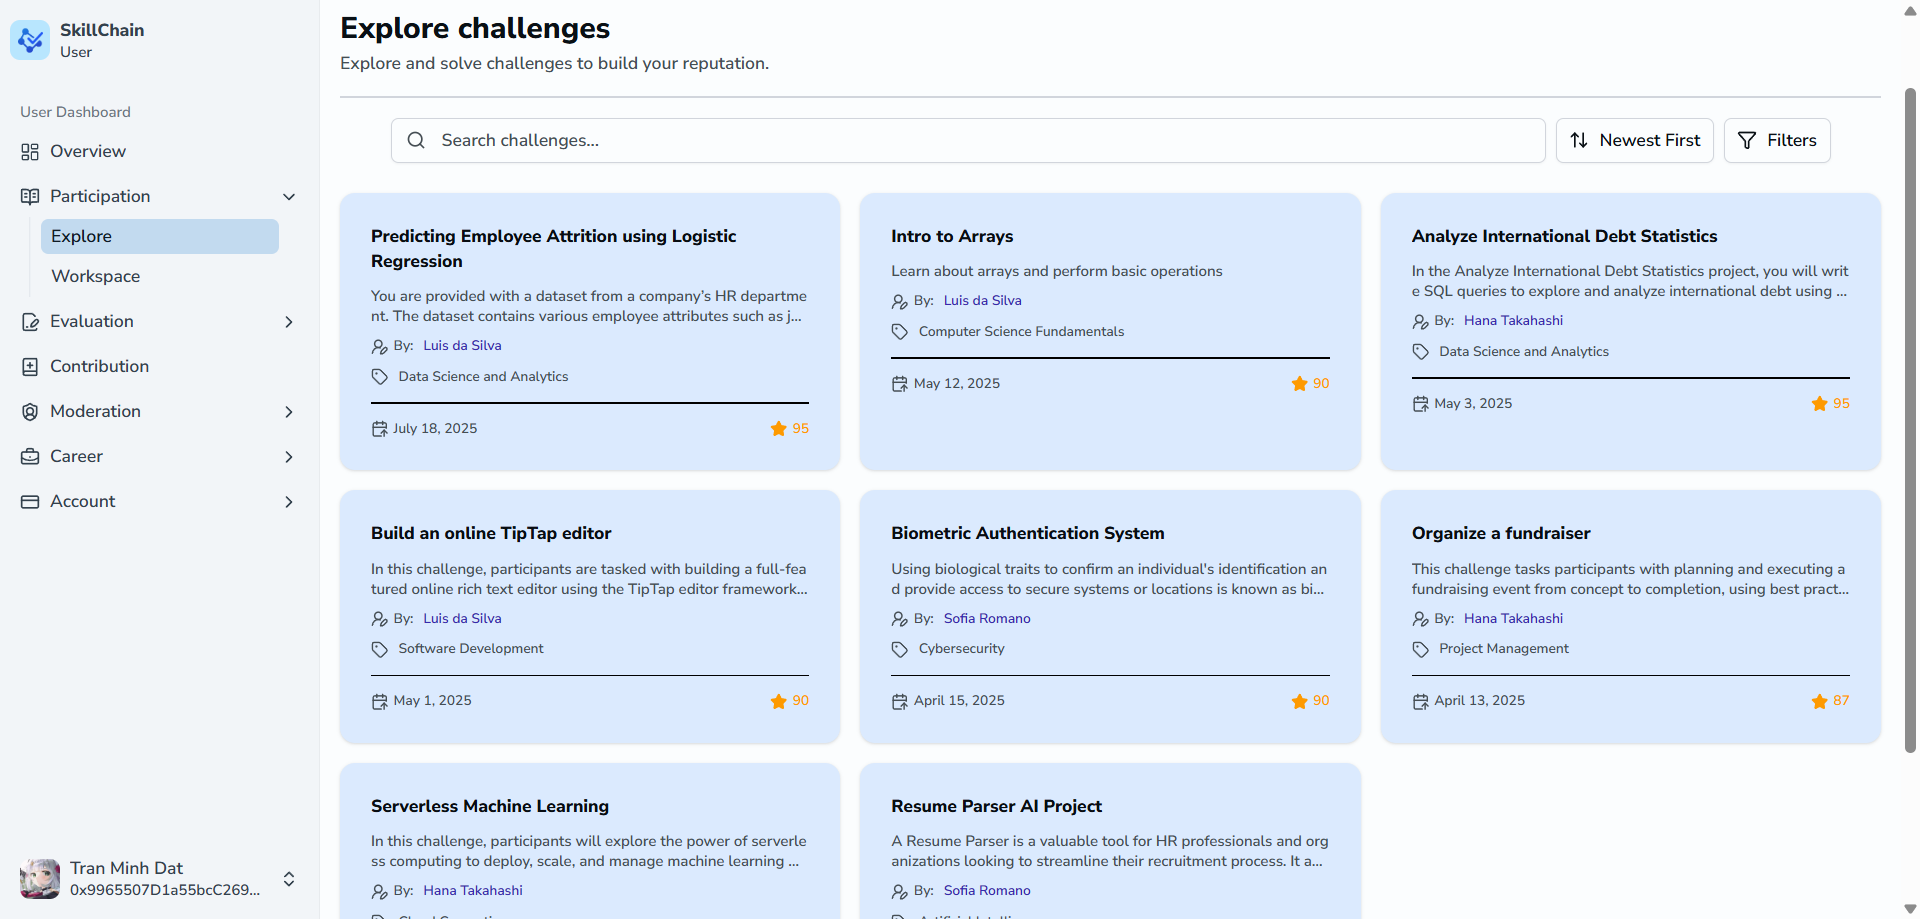
\includegraphics[width=0.99\textwidth, frame]{ui/explore-challenges-page.png}
  \caption{Trang danh sách thử thách đang hiện hành}
  \label{fig:explore-challenges-page}
\end{figure}

\subsubsection{Thực hiện thử thách}

Khi xem chi tiết nội dung một thử thách, người dùng có thể nhấn nút ``Join Challenge'' (ở góc trên hoặc góc dưới bên phải) để tham gia.  
Hệ thống sẽ yêu cầu người dùng xác nhận trả một khoản phí và xác thực giao dịch qua ví tiền điện tử.

\begin{figure}[H]
  \centering
  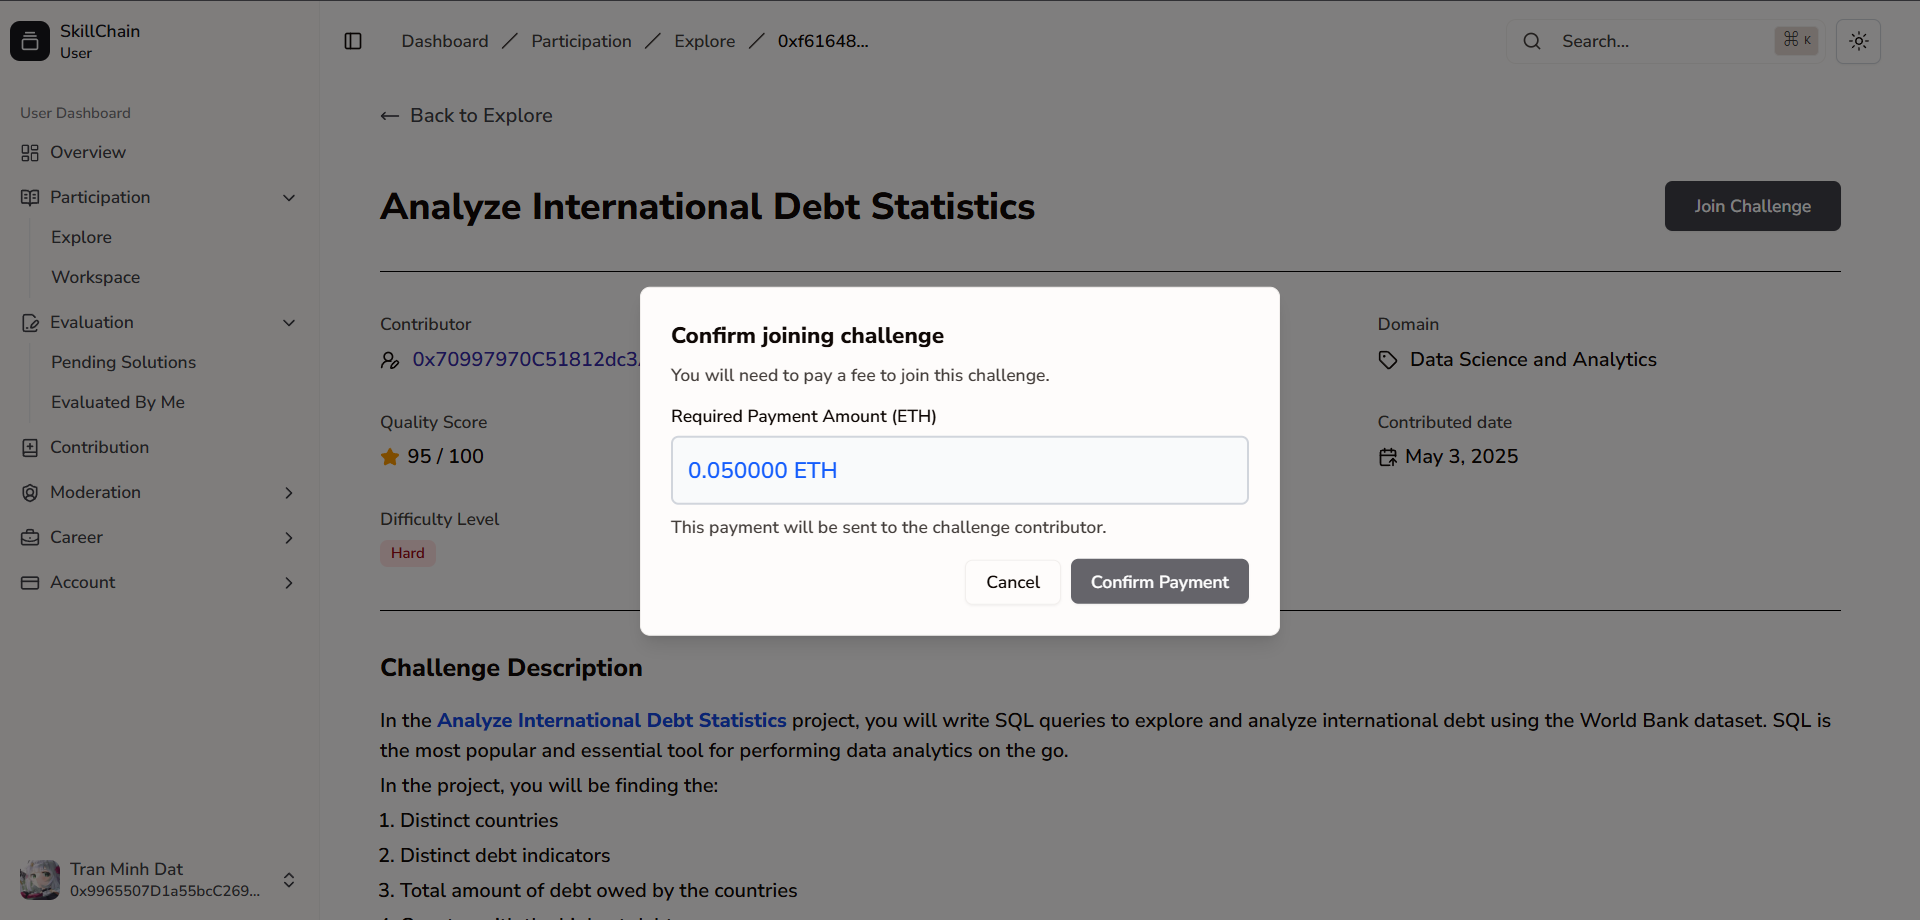
\includegraphics[width=0.99\textwidth, frame]{ui/join-challenge-payment-dialog.png}
  \caption{Xác nhận trả phí tham gia thử thách}
  \label{fig:join-challenge-payment-dialog}
\end{figure}

Sau khi tham gia thành công, người dùng truy cập \textbf{Participation} $\rightarrow$ \textbf{Workspace} để xem các thử thách đã và đang tham gia.  
Tại đây, người dùng có thể bắt đầu xây dựng giải pháp. Hệ thống cho phép lưu tạm giải pháp nhiều lần trước khi nộp chính thức.

\begin{figure}[H]
  \centering
  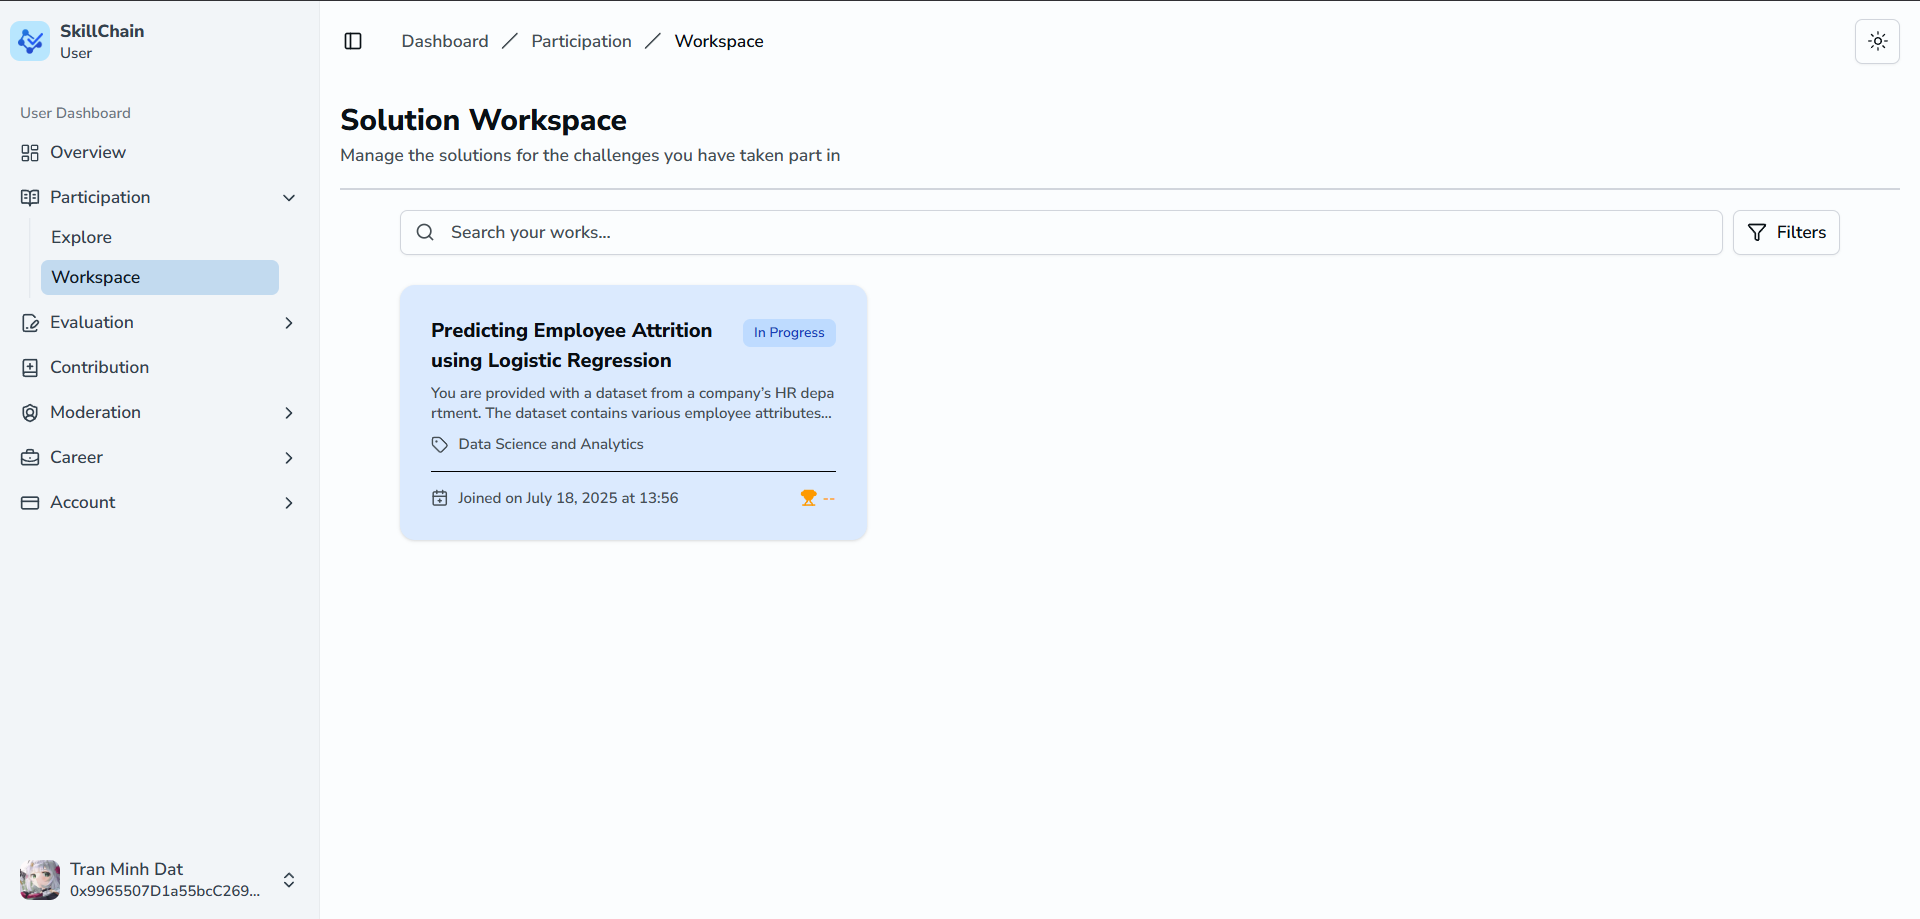
\includegraphics[width=0.99\textwidth, frame]{ui/workspace-challenge-page.png}
  \caption{Trang danh sách thử thách đã tham gia}
  \label{fig:workspace-challenge-page}
\end{figure}

\begin{figure}[H]
  \centering
  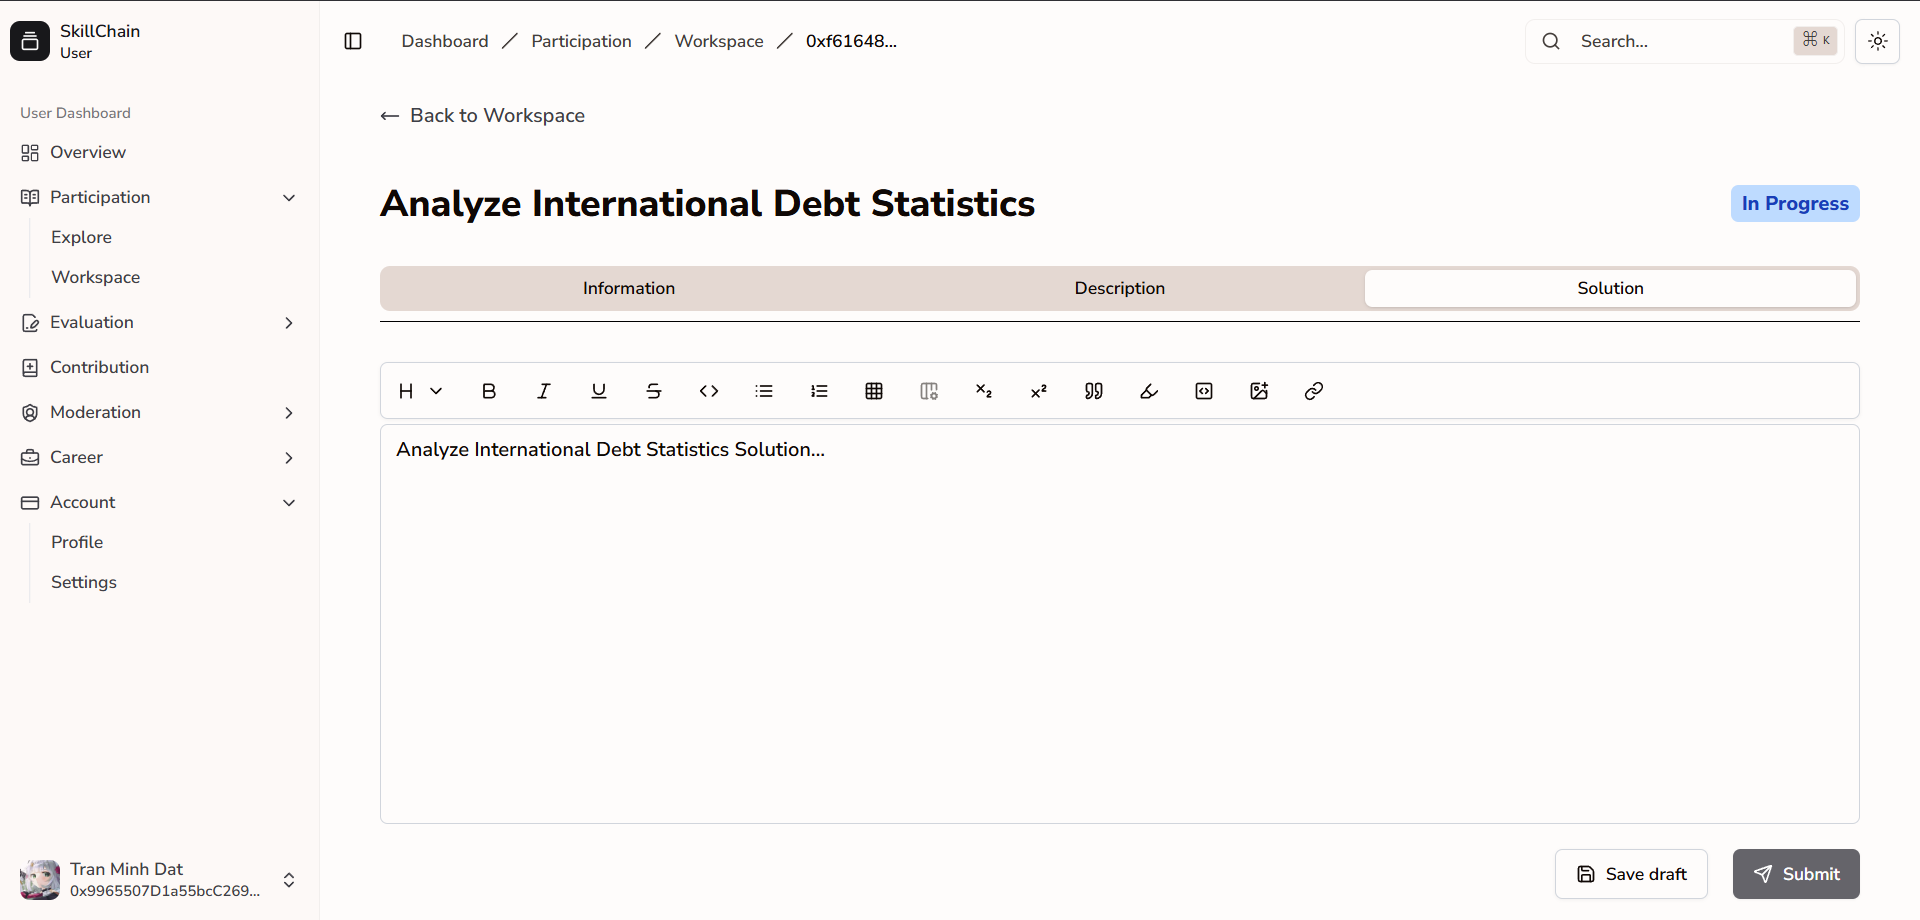
\includegraphics[width=0.99\textwidth, frame]{ui/solution-workspace-page.png}
  \caption{Không gian soạn thảo giải pháp}
  \label{fig:solution-workspace-page}
\end{figure}

Sau khi hoàn thiện giải pháp, người dùng nhấn nút ``Submit'' để nộp bài. Kể từ thời điểm này, nội dung giải pháp sẽ bị khóa và không thể chỉnh sửa.
Khi đã sẵn sàng gửi bài để chấm điểm, người dùng nhấn ``Put Under Review''. Mỗi hành động nộp bài hoặc gửi đánh giá đều yêu cầu xác thực giao dịch thông qua ví tiền điện tử.

\begin{figure}[H]
  \centering
  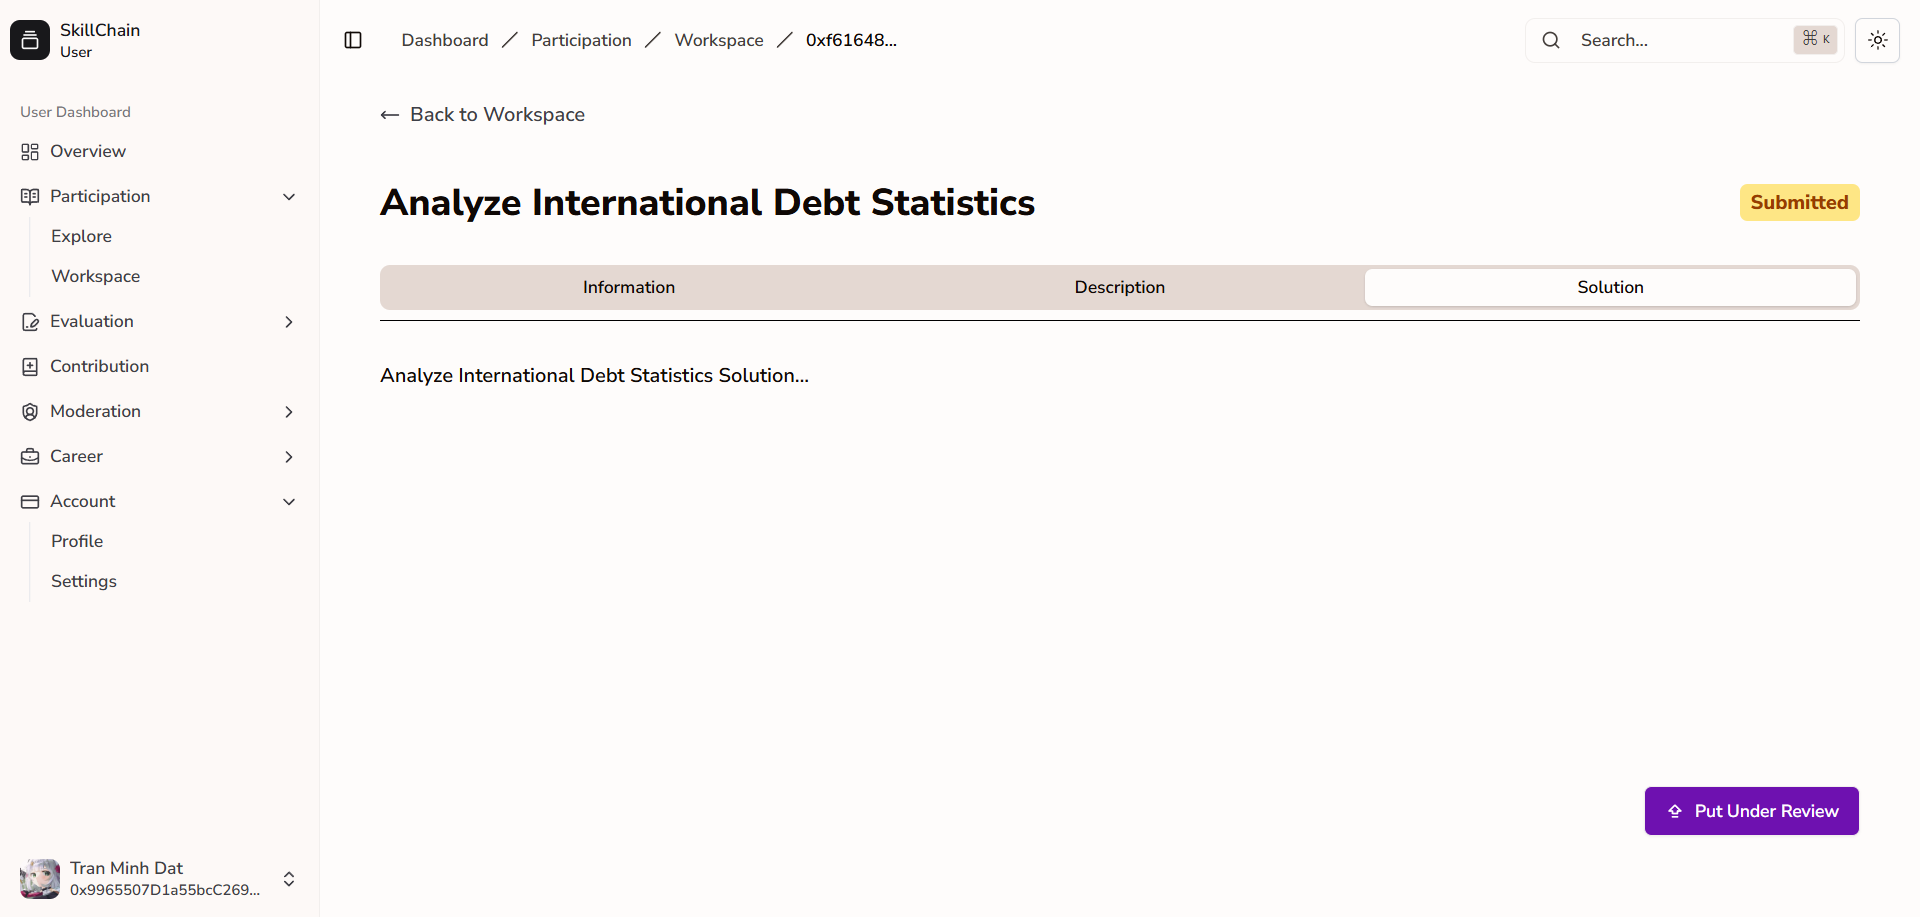
\includegraphics[width=0.99\textwidth, frame]{ui/submitted-solution-page.png}
  \caption{Giải pháp đã được nộp}
  \label{fig:submitted-solution-page}
\end{figure}

\subsection{Trang đánh giá giải pháp}

\subsubsection{Xem giải pháp đang chờ đánh giá}

Để xem danh sách các giải pháp đang chờ đánh giá, người dùng truy cập \textbf{Evaluation} $\rightarrow$ \textbf{Pending Solution}.  
Tại đây, hệ thống hiển thị các giải pháp đang chờ đánh giá, bao gồm tên người nộp giải, số lượng người đánh giá đã tham gia.  
Tuy nhiên, nội dung chi tiết của giải pháp sẽ chưa được hiển thị ở giai đoạn này.

\begin{figure}[H]
  \centering
  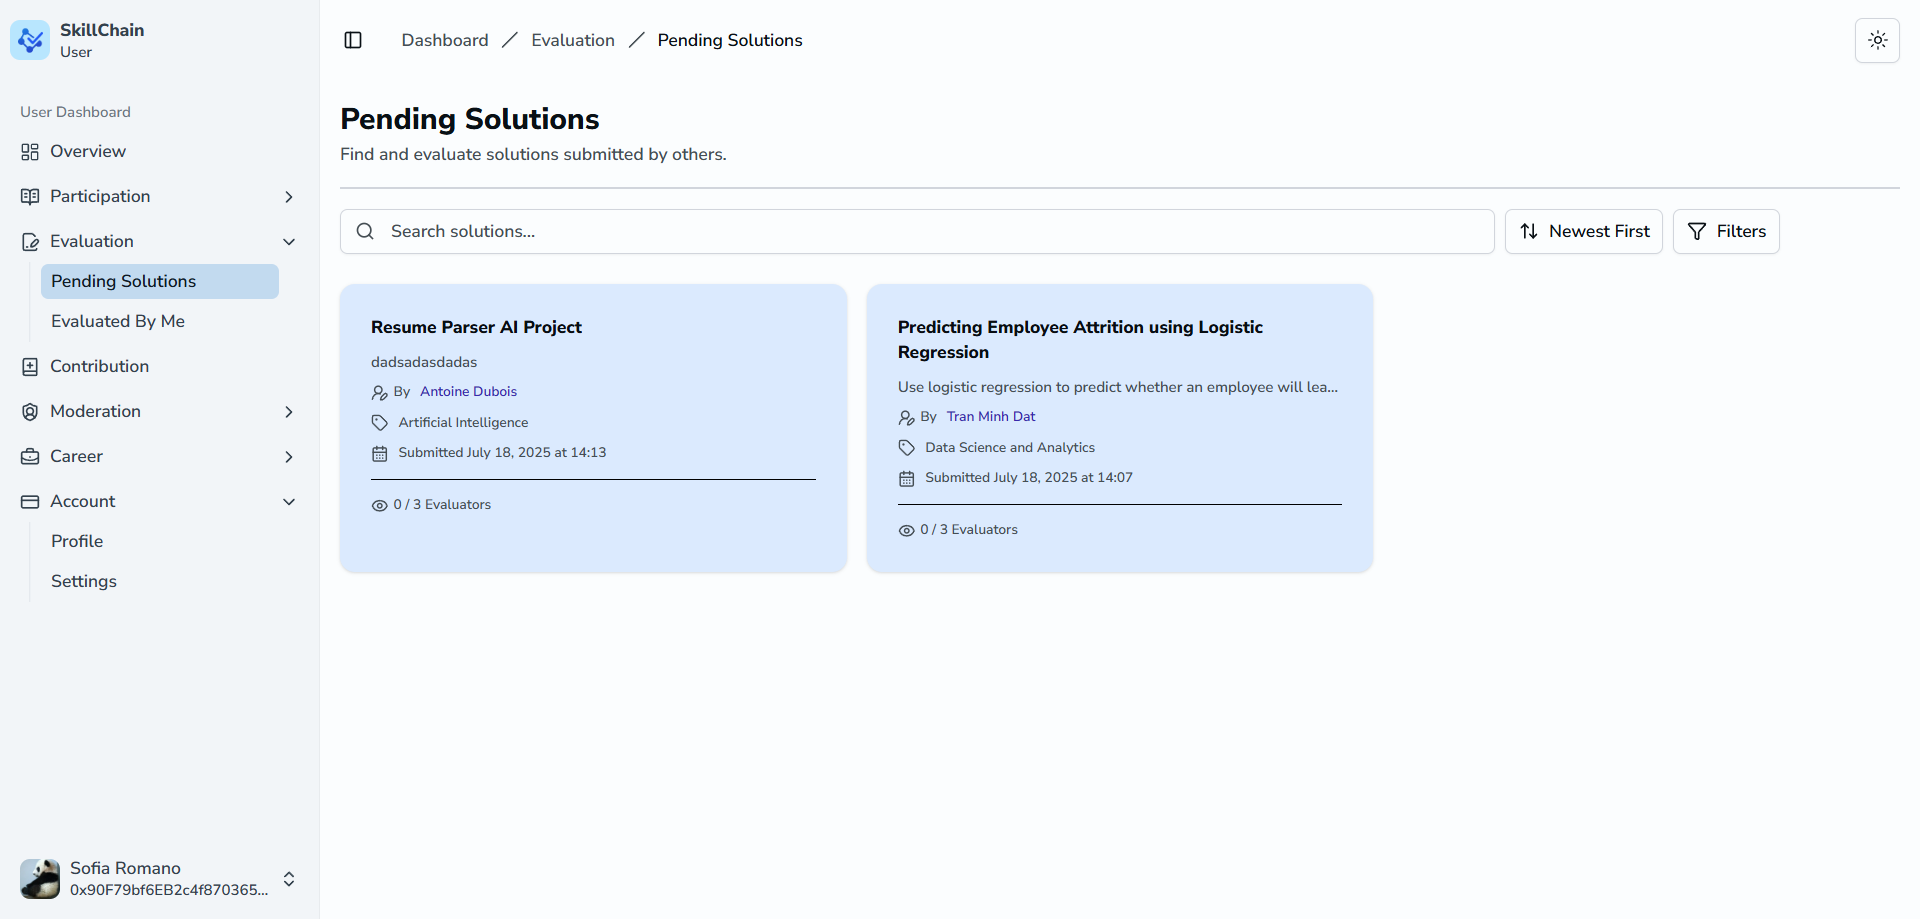
\includegraphics[width=0.99\textwidth, frame]{ui/pending-solution-page.png}
  \caption{Trang danh sách giải pháp đang chờ đánh giá}
  \label{fig:pending-solution-page}
\end{figure}

\subsubsection{Tham gia đánh giá giải pháp}

Khi xem thông tin chi tiết của một giải pháp, người dùng có thể nhấn nút ``Evaluate Solution'' để đăng ký tham gia đánh giá.  
Hệ thống sẽ yêu cầu xác thực giao dịch thông qua ví tiền điện tử để xác nhận quyền đánh giá.
Nếu người dùng không đủ chỉ số uy tín chuyên môn phù hợp với loại thử thách, hệ thống sẽ hiển thị thông báo lỗi và không cho phép tiếp tục.

\begin{figure}[H]
  \centering
  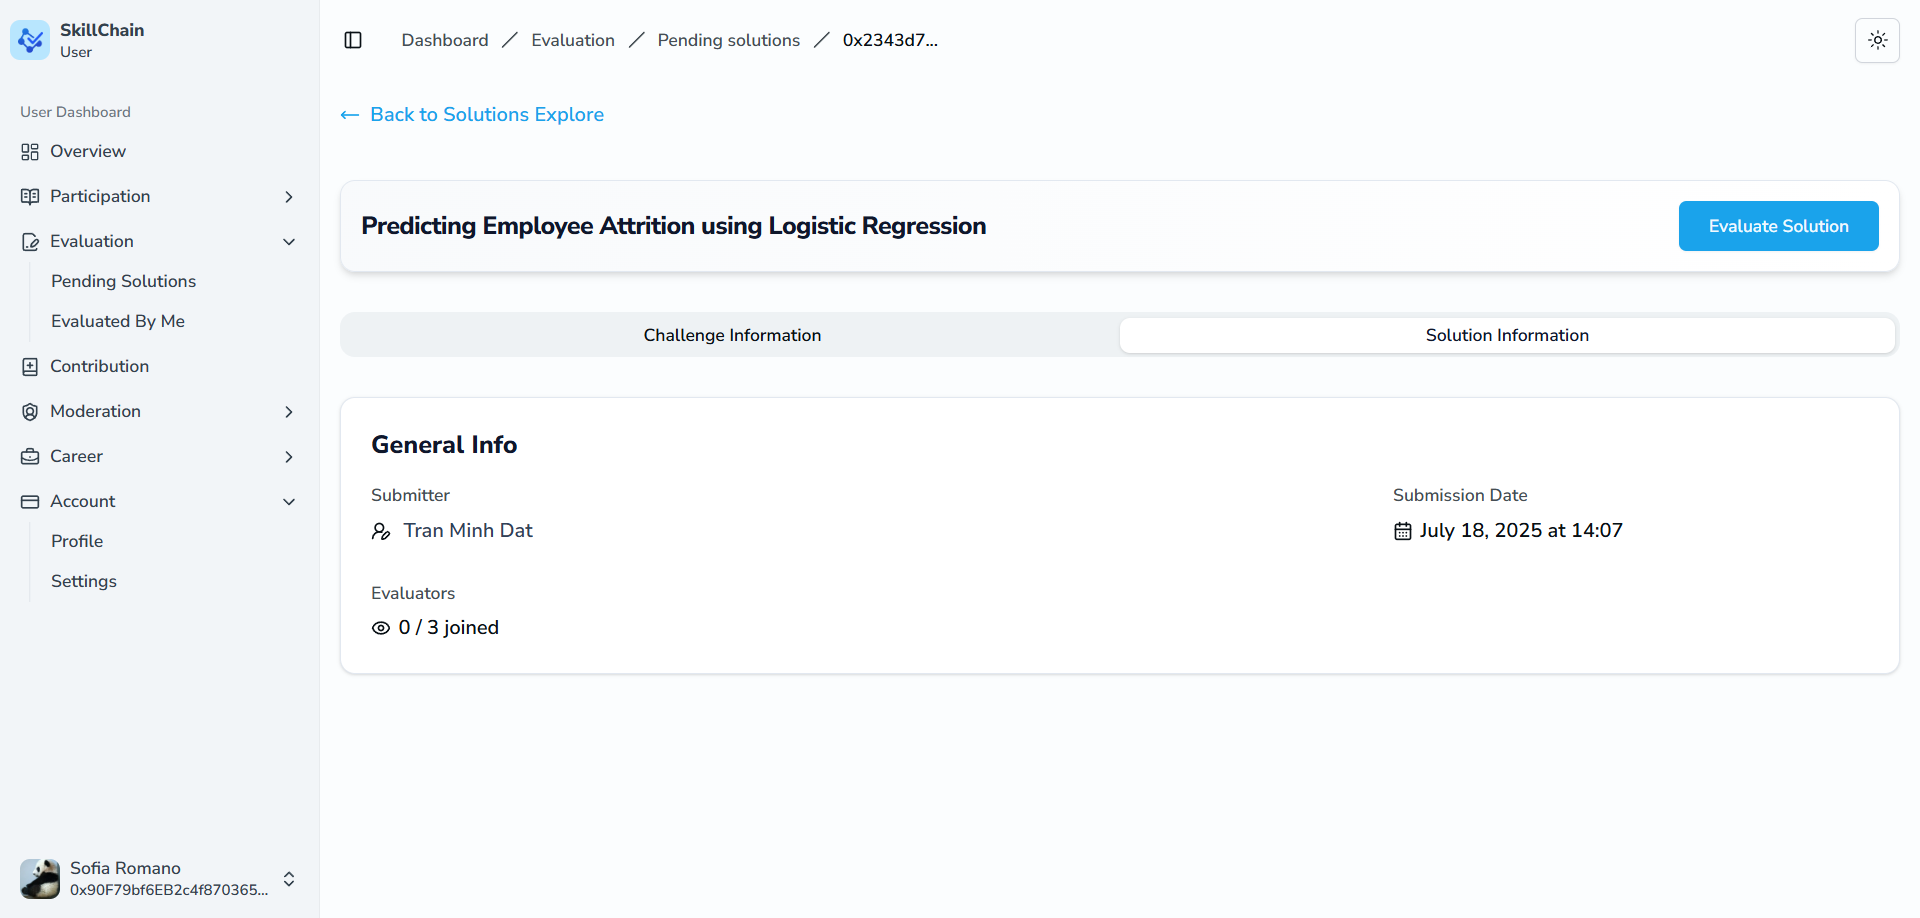
\includegraphics[width=0.99\textwidth, frame]{ui/pending-solution-info-page.png}
  \caption{Thông tin cơ bản của giải pháp đang chờ đánh giá}
  \label{fig:pending-solution-info-page}
\end{figure}

\subsubsection{Thực hiện đánh giá giải pháp}

Sau khi tham gia đánh giá, người dùng truy cập \textbf{Evaluation} $\rightarrow$ \textbf{Evaluated By Me} để xem danh sách các giải pháp mà mình đã hoặc đang đánh giá.  
Tại đây, người đánh giá có thể xem nội dung chi tiết của giải pháp và tiến hành chấm điểm.

\begin{figure}[H]
  \centering
  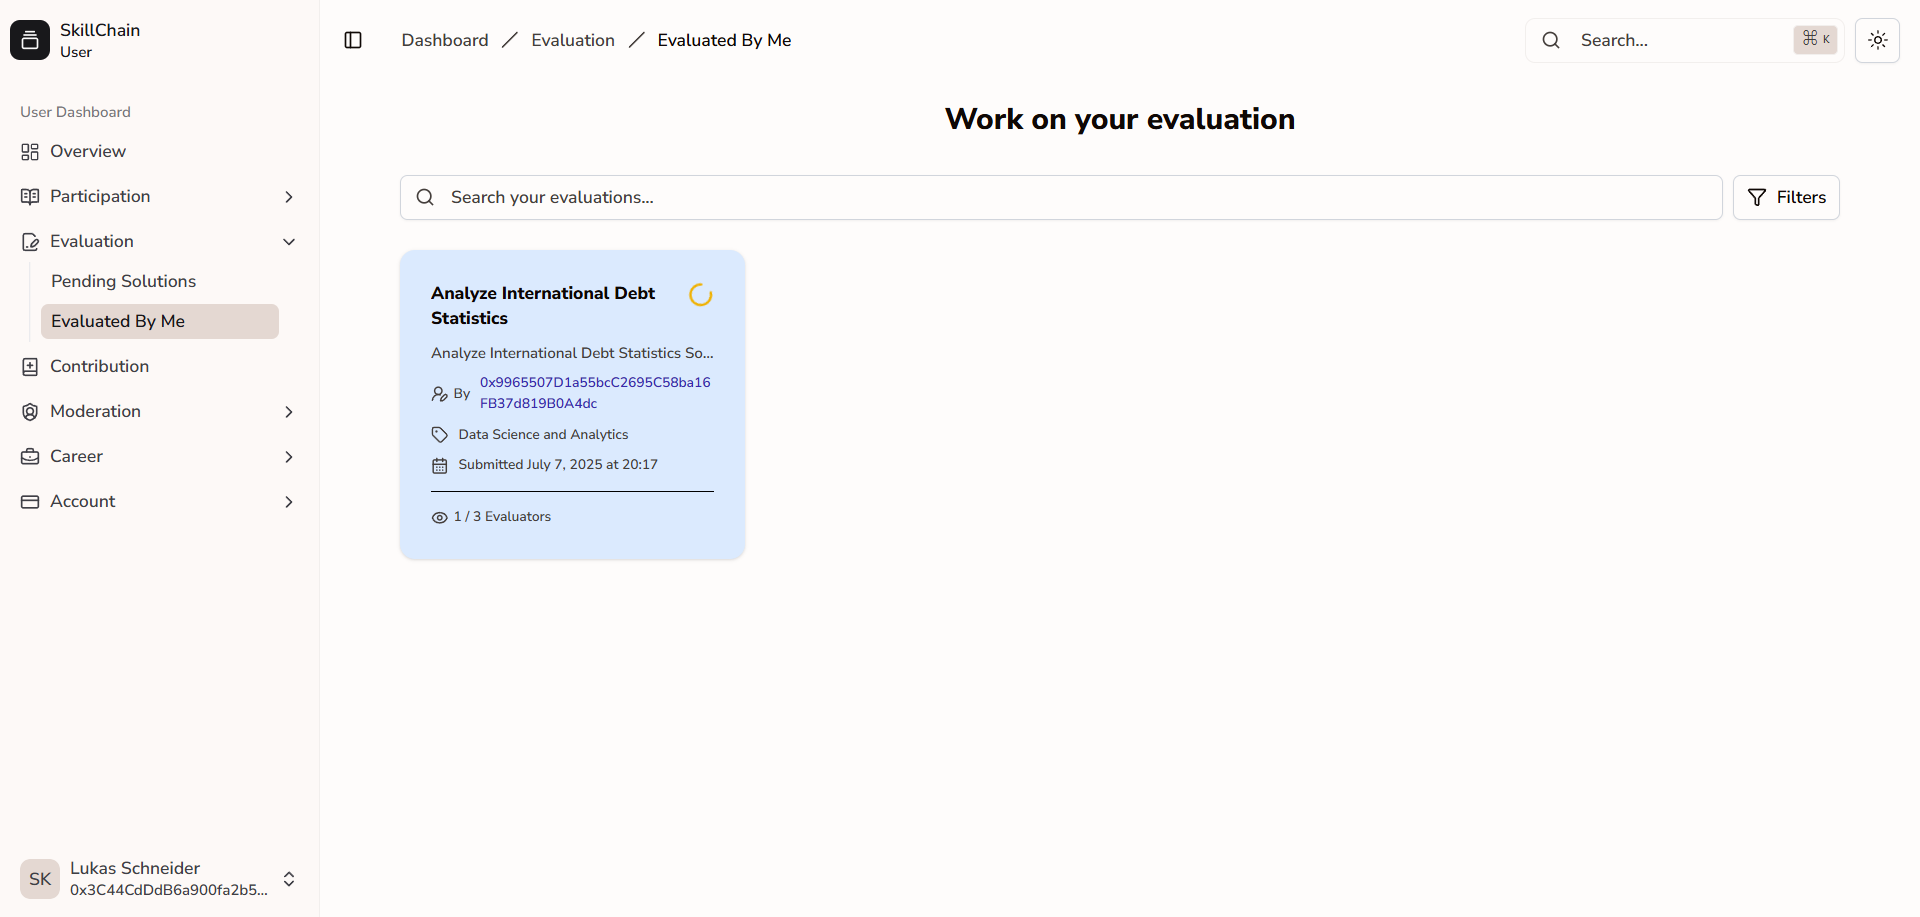
\includegraphics[width=0.99\textwidth, frame]{ui/evaluated-by-me-page.png}
  \caption{Trang danh sách giải pháp đã và đang đánh giá}
  \label{fig:evaluated-by-me-page}
\end{figure}

Người dùng thực hiện đánh giá bằng cách điền nội dung nhận xét, chấm điểm theo thang điểm quy định và nhấn ``Submit'' để nộp kết quả.  
Sau khi gửi đi, kết quả đánh giá sẽ được khóa và không thể chỉnh sửa.

\begin{figure}[H]
  \centering
  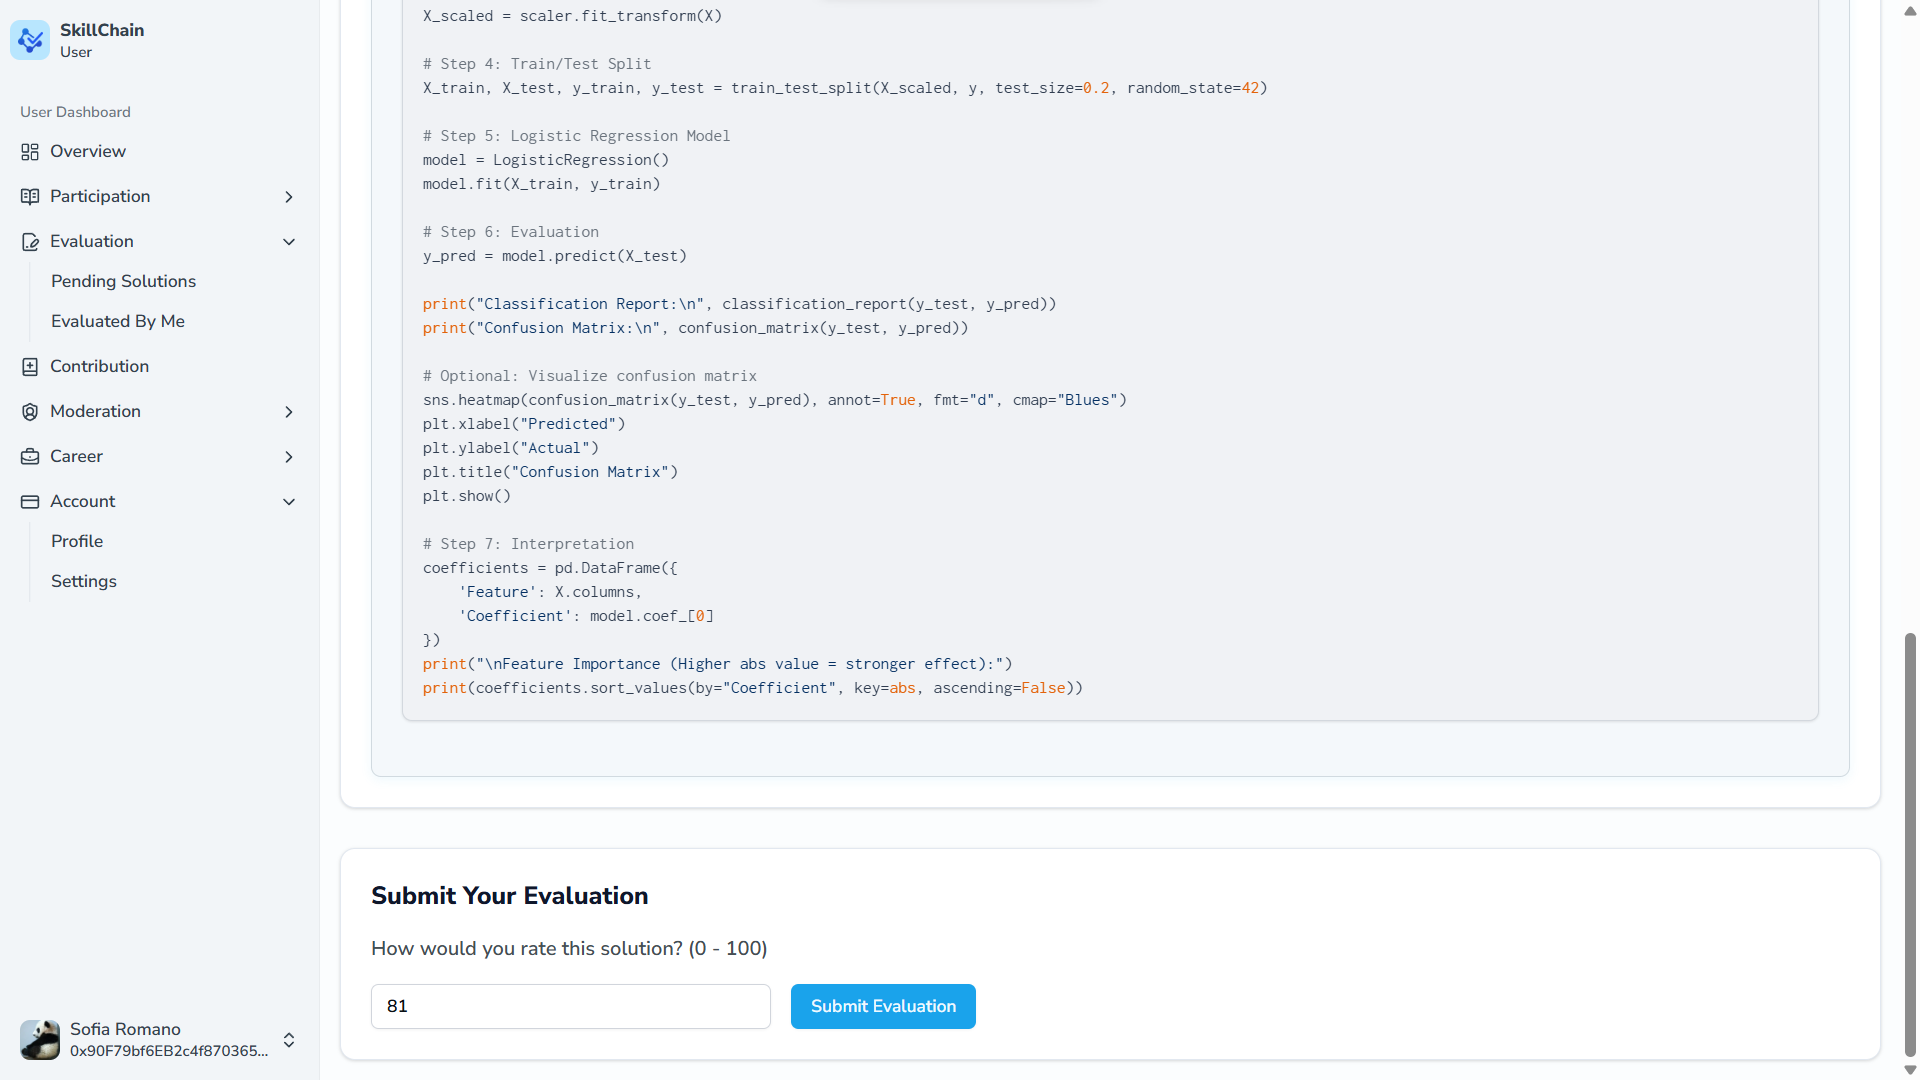
\includegraphics[width=0.99\textwidth, frame]{ui/evaluate-solution-page.png}
  \caption{Trang thực hiện đánh giá giải pháp}
  \label{fig:evaluate-solution-page}
\end{figure}

Sau khi quá trình đánh giá hoàn tất, hệ thống sẽ công khai kết quả phiên đánh giá cho cả người giải và các người đánh giá cũng như cập nhật số người hoàn thành thử thách. 

\begin{figure}[H]
  \centering
  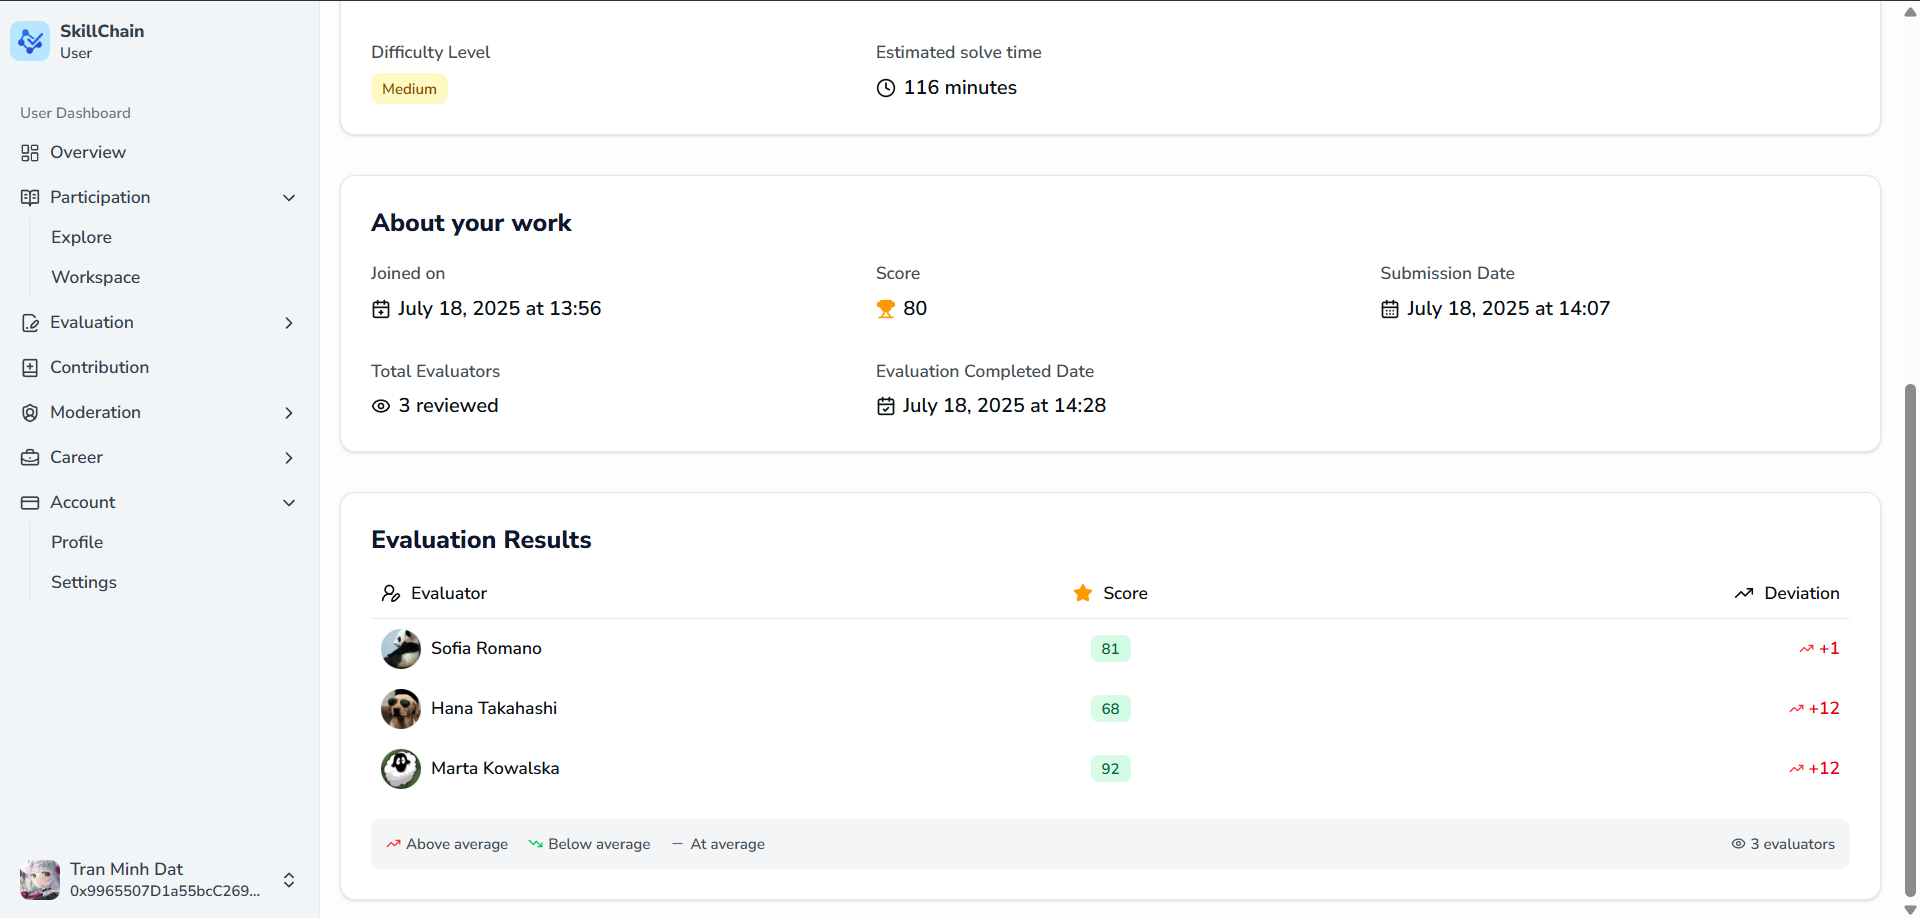
\includegraphics[width=0.99\textwidth, frame]{ui/evaluated-solution-page.png}
  \caption{Giải pháp đã được đánh giá hoàn tất}
  \label{fig:evaluated-solution-page}
\end{figure}

\section{Giao diện tuyển dụng nhân sự}

\subsection{Truy cập không gian nhà tuyển dụng}

Để chuyển sang không gian nhà tuyển dụng, người dùng kết nối ví như thông thường.  
Tại thanh thông tin cá nhân (góc trái bên dưới giao diện), nhấn vào biểu tượng tài khoản và chọn tùy chọn ``Switch to Recruiter''.  
Hệ thống sẽ tự động điều hướng sang không gian làm việc dành riêng cho nhà tuyển dụng.

\begin{figure}[H]
  \centering
  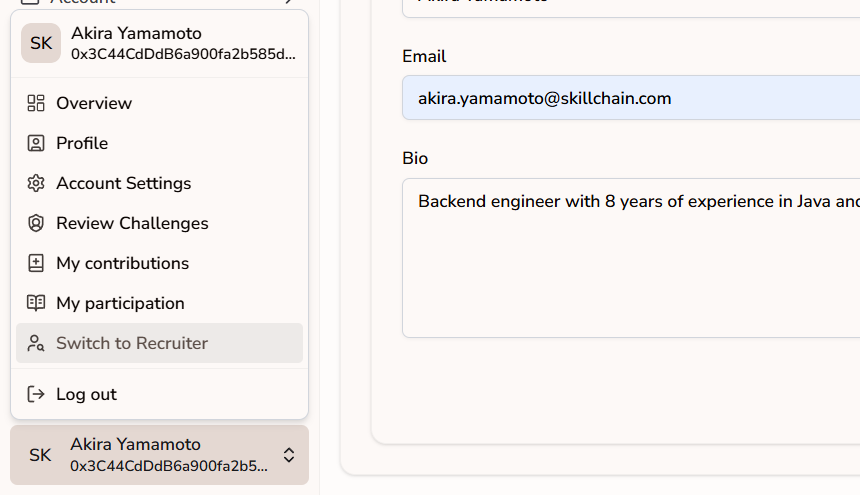
\includegraphics[width=0.99\textwidth, frame]{ui/access-recruiter-space.png}
  \caption{Truy cập không gian nhà tuyển dụng}
  \label{fig:access-recruiter-space}
\end{figure}

\subsection{Trang tài khoản nhà tuyển dụng}

Tại không gian nhà tuyển dụng, người dùng truy cập tab \textbf{Account} để quản lý hồ sơ cá nhân, thông tin công ty, cũng như thiết lập cấu hình liên quan đến quá trình tuyển dụng.

\subsubsection{Đăng ký trở thành nhà tuyển dụng}

Để sử dụng tính năng tuyển dụng, hệ thống yêu cầu người dùng ký gửi tối thiểu \textbf{1 ETH}.  
Để thực hiện, nhà tuyển dụng truy cập tab \textbf{Account Settings}, nhập số ETH muốn gửi tại mục ``Recruiter Budget'' và nhấn nút ``Deposit''.  
Sau đó, xác nhận giao dịch thông qua ví tiền điện tử.  
Các chi phí phát sinh trong quá trình tuyển dụng sẽ tự động được khấu trừ từ khoản ký gửi này.

\begin{figure}[H]
  \centering
  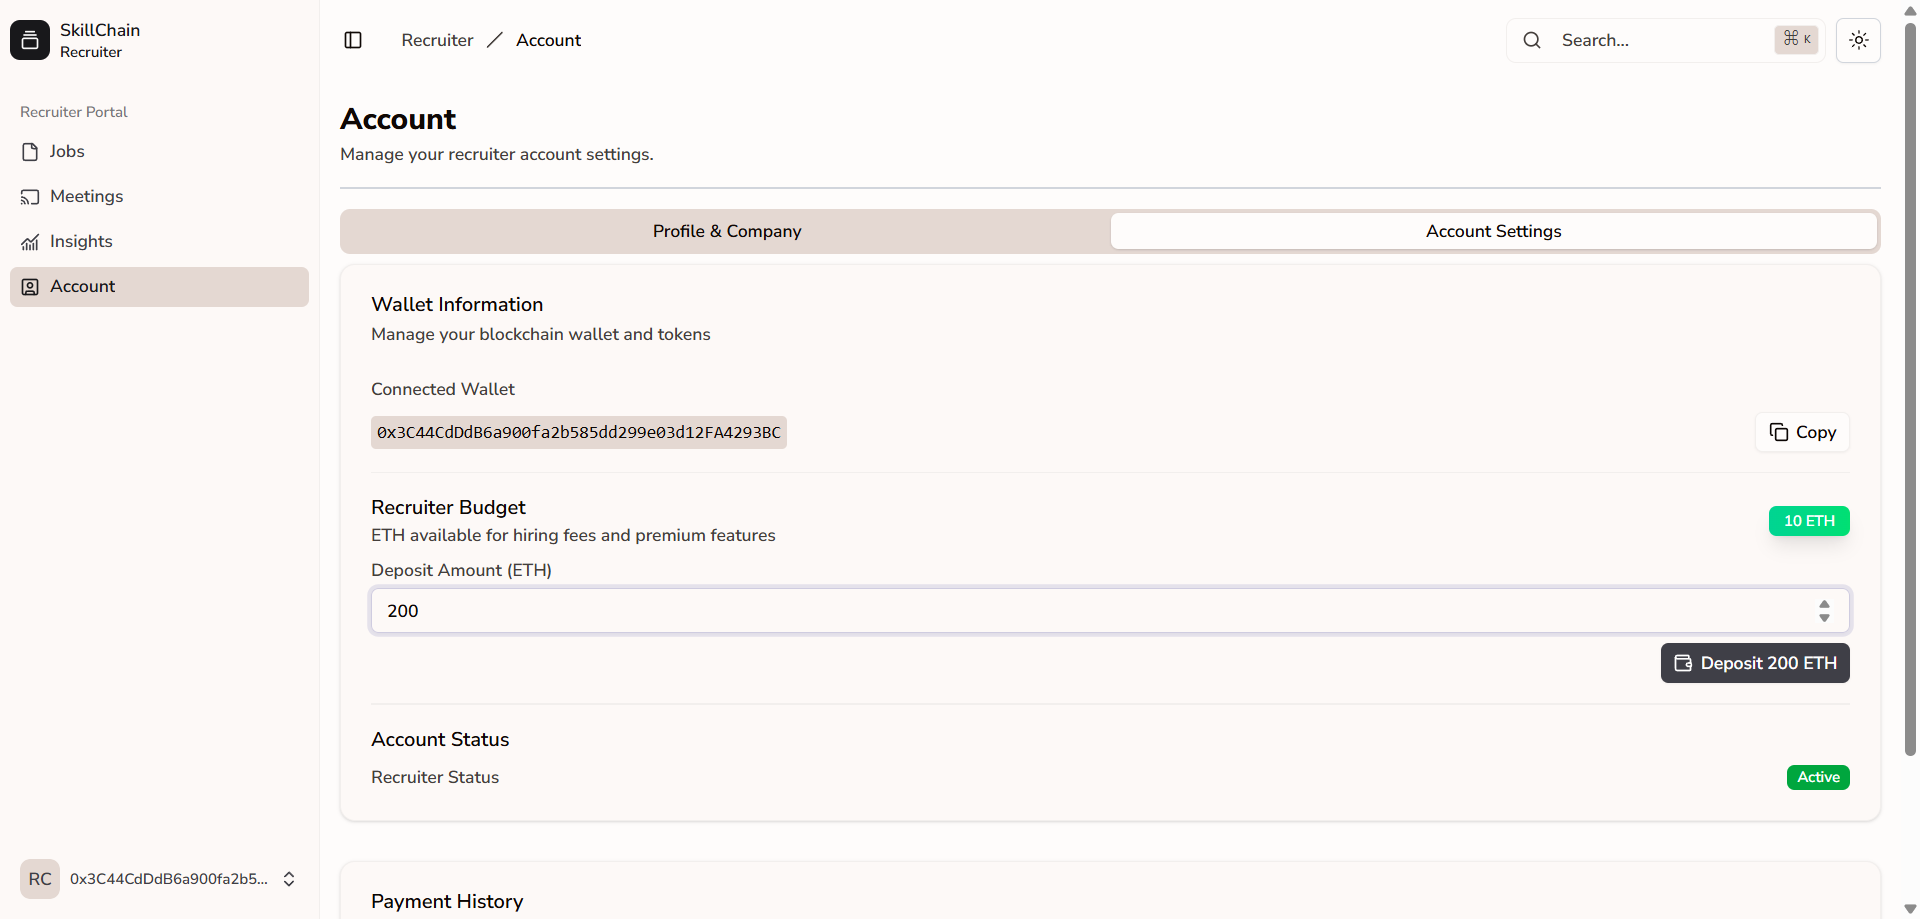
\includegraphics[width=0.99\textwidth, frame]{ui/recruiter-account-settings-page.png}
  \caption{Trang thiết lập tài khoản nhà tuyển dụng}
  \label{fig:recruiter-account-settings-page}
\end{figure}

\subsubsection{Quản lý hồ sơ nhà tuyển dụng}

Tại tab \textbf{Profile \& Company}, nhà tuyển dụng có thể đăng ký hoặc cập nhật hồ sơ cá nhân và thông tin công ty.  
Trong lần truy cập đầu tiên, hệ thống yêu cầu xác thực giao dịch qua ví điện tử để hoàn tất đăng ký.

\begin{figure}[H]
  \centering
  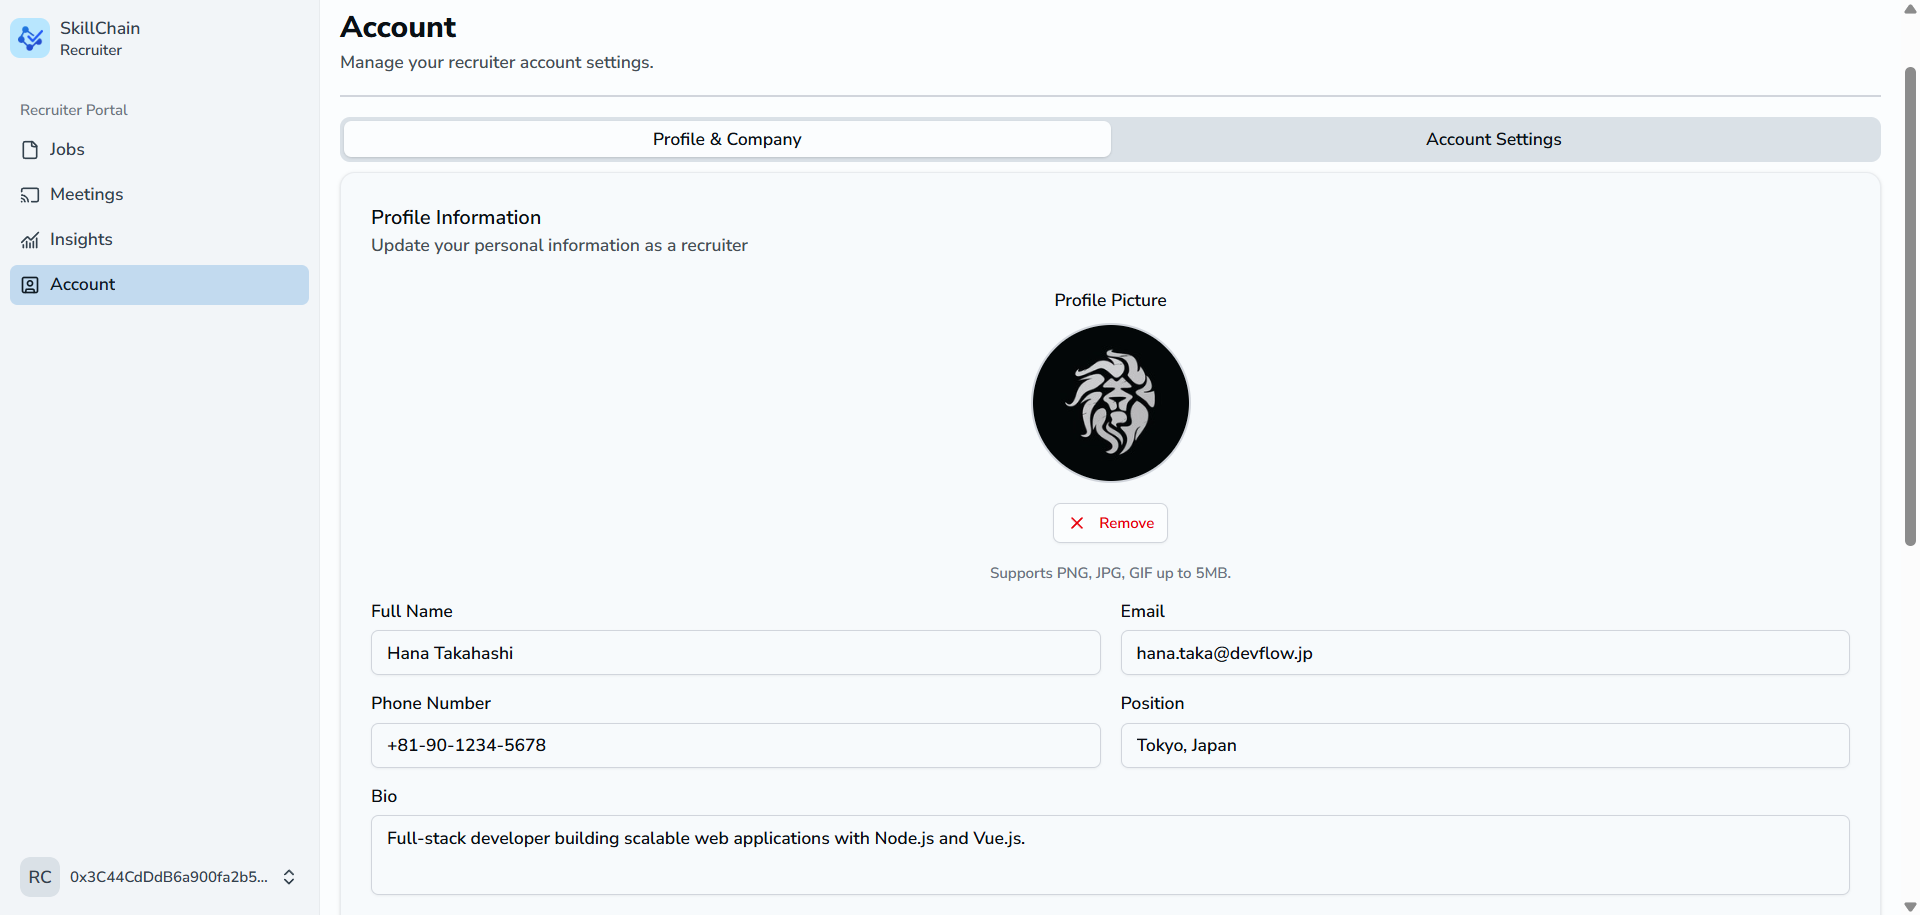
\includegraphics[width=0.99\textwidth, frame]{ui/recruiter-personal-profile.png}
  \caption{Hồ sơ cá nhân nhà tuyển dụng}
  \label{fig:recruiter-personal-profile}
\end{figure}

\begin{figure}[H]
  \centering
  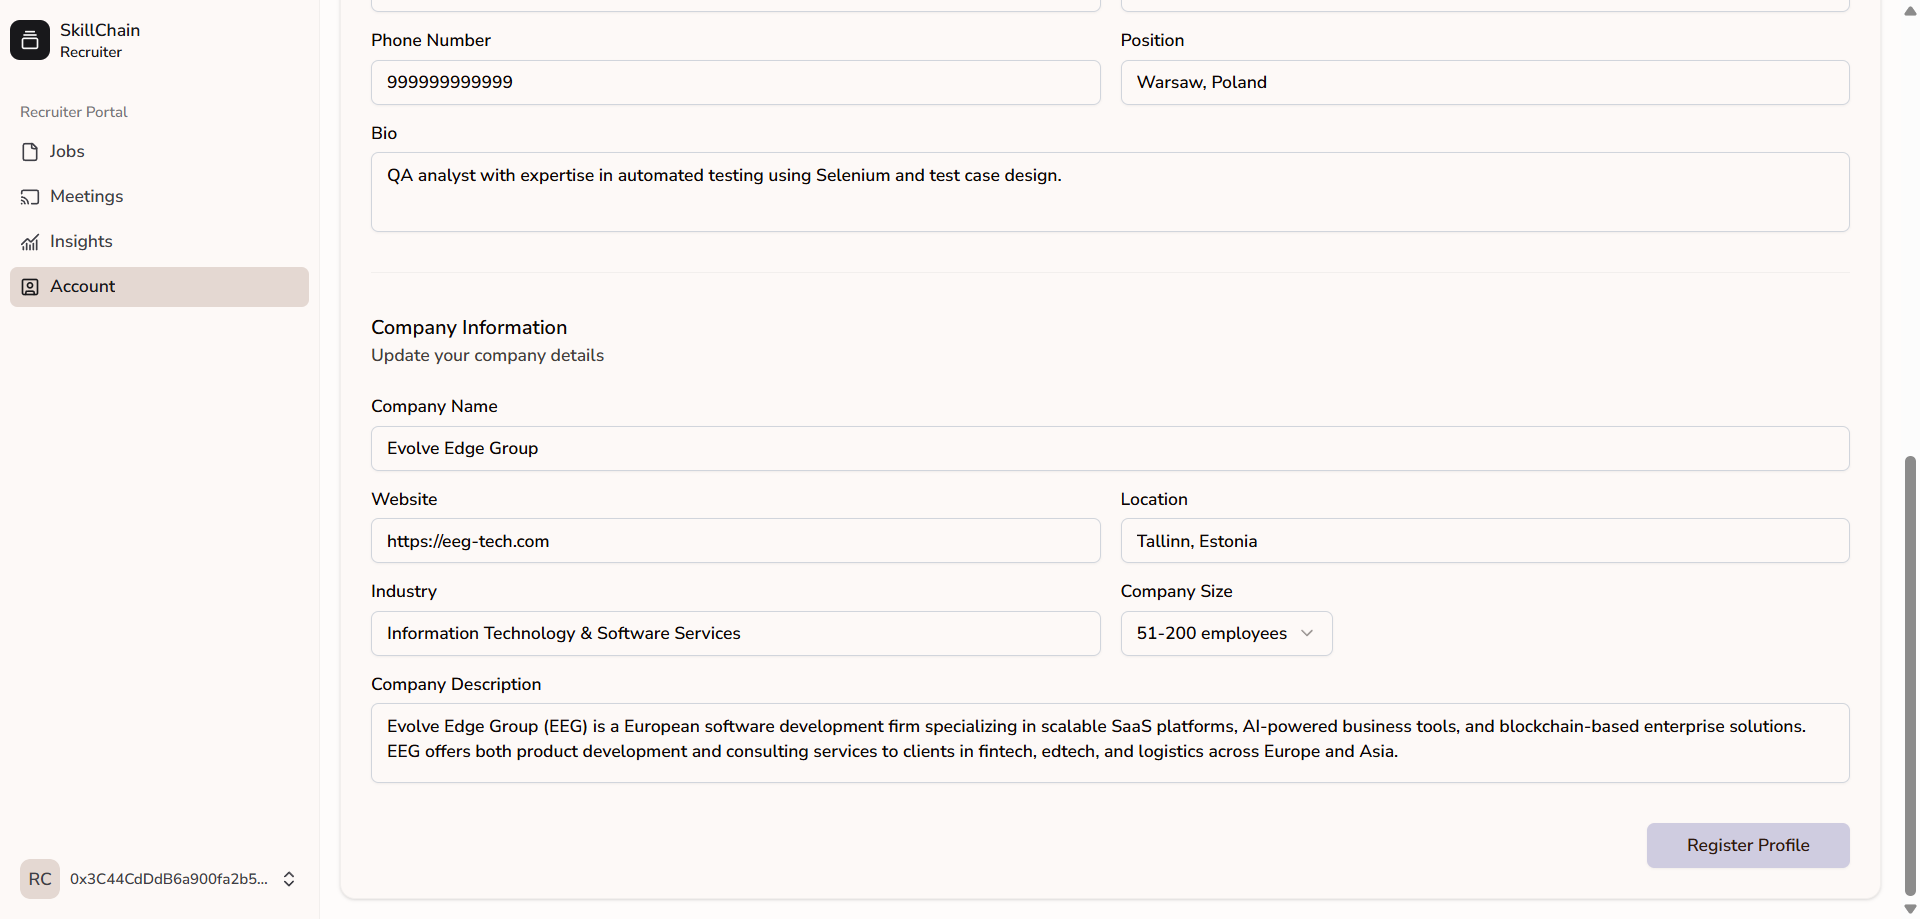
\includegraphics[width=0.99\textwidth, frame]{ui/recruiter-company-profile.png}
  \caption{Thông tin công ty của nhà tuyển dụng}
  \label{fig:recruiter-company-profile}
\end{figure}

\subsection{Trang quản lý bài đăng}

\subsubsection{Xem danh sách các bài đăng tuyển dụng}

Để xem danh sách các bài đăng tuyển dụng, nhà tuyển dụng truy cập tab \textbf{Jobs}.  
Tại đây, hệ thống hiển thị danh sách các bài đăng đã tạo cùng với thông tin trạng thái, số lượng ứng viên đã ứng tuyển và các hành động có thể thực hiện.

\begin{figure}[H]
  \centering
  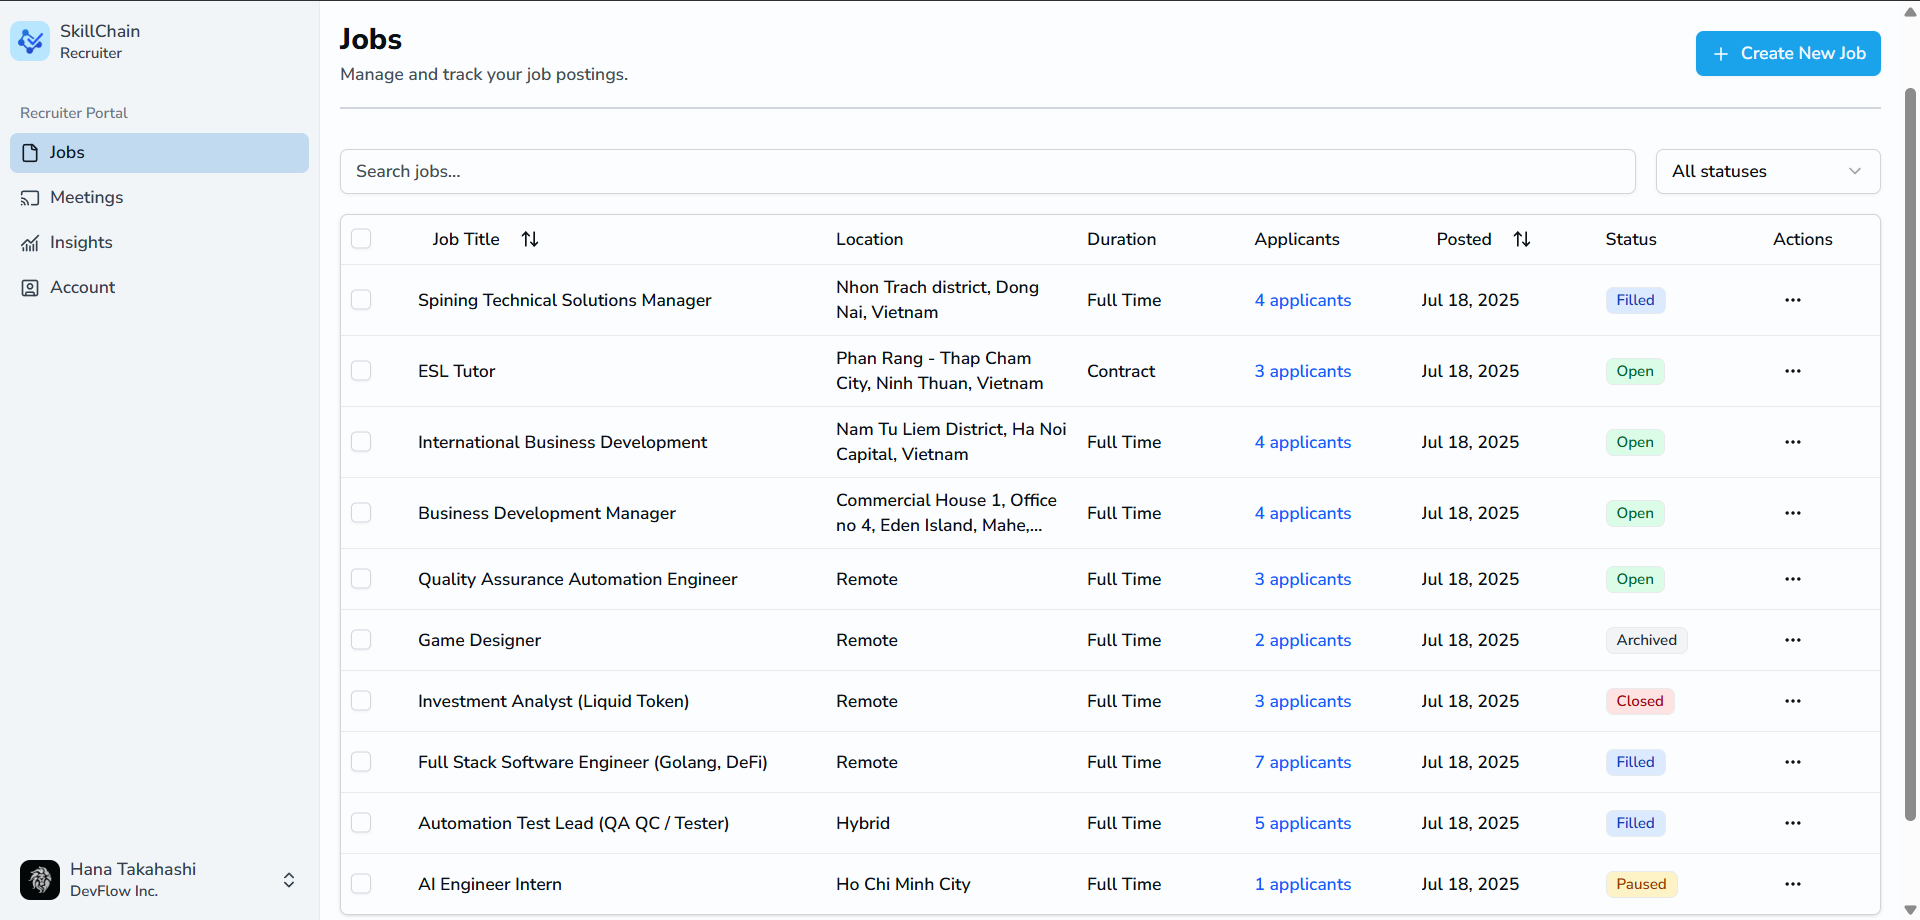
\includegraphics[width=0.99\textwidth, frame]{ui/jobs-page.png}
  \caption{Trang danh sách các bài đăng tuyển dụng}
  \label{fig:jobs-page}
\end{figure}

Để xem chi tiết một bài đăng, nhà tuyển dụng nhấn ``View job'' tại nút ``Actions'' tương ứng.

\begin{figure}[H]
  \centering
  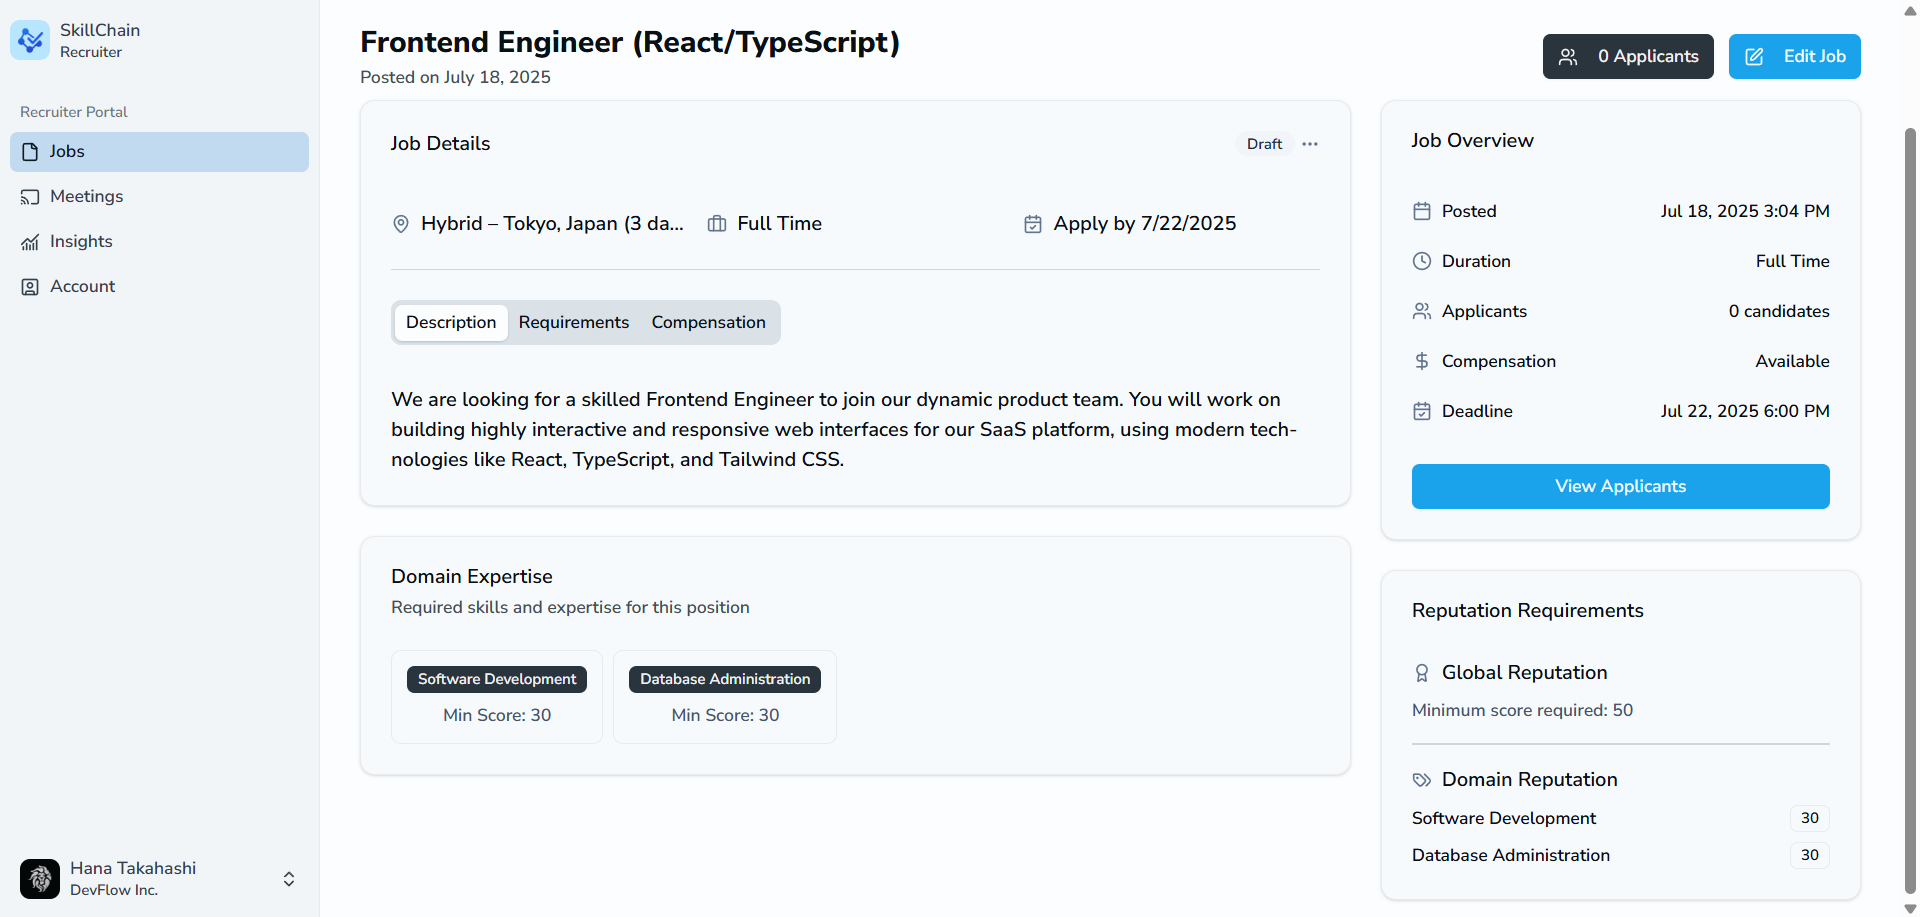
\includegraphics[width=0.99\textwidth, frame]{ui/job-detail-page.png}
  \caption{Trang chi tiết một bài đăng tuyển dụng}
  \label{fig:job-detail-page}
\end{figure}

\subsubsection{Tạo bài đăng tuyển dụng mới}

Để tạo bài đăng mới, nhà tuyển dụng nhấn nút ``Create New Job'' ở góc trên bên phải.  
Tại giao diện tạo bài đăng, nhà tuyển dụng nhập thông tin vị trí công việc, thời hạn đăng bài, cùng với các yêu cầu về uy tín đối với ứng viên.  
Sau khi hoàn tất, nhấn nút ``Create Job'' và xác nhận giao dịch qua ví điện tử để tạo bài đăng ở trạng thái nháp.

\begin{figure}[H]
  \centering
  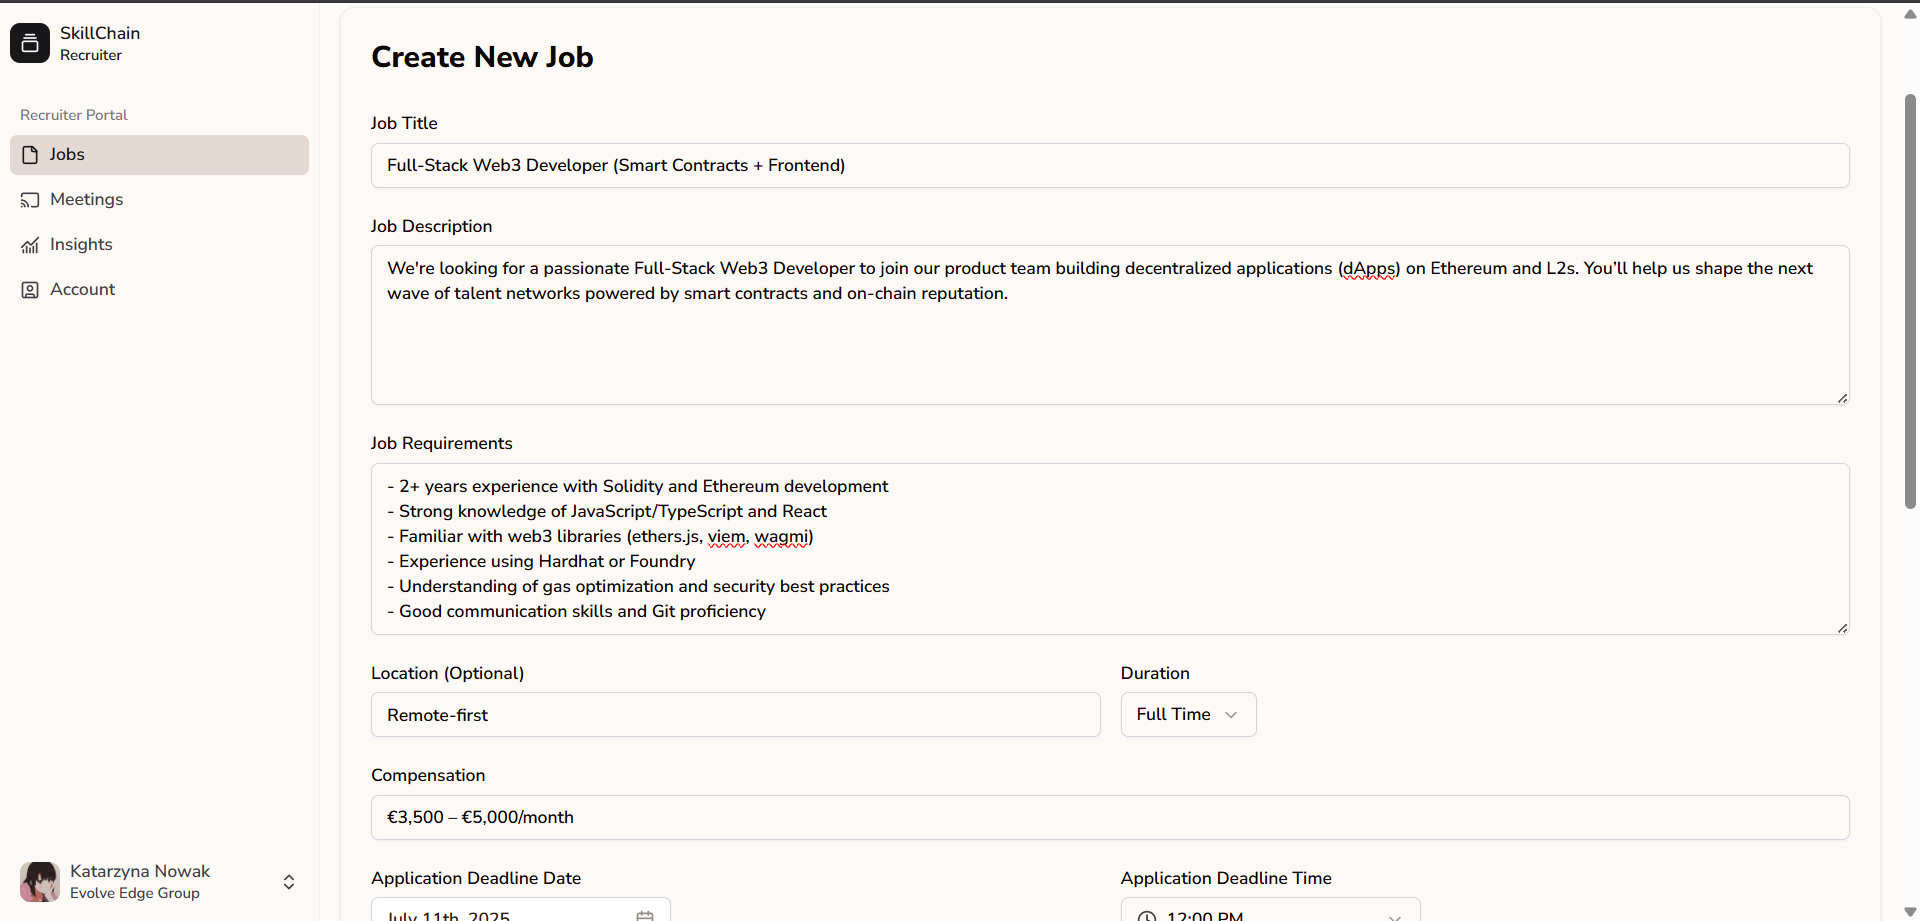
\includegraphics[width=0.99\textwidth, frame]{ui/job-position-info.png}
  \caption{Thông tin về vị trí công việc}
  \label{fig:job-position-info}
\end{figure}

\begin{figure}[H]
  \centering
  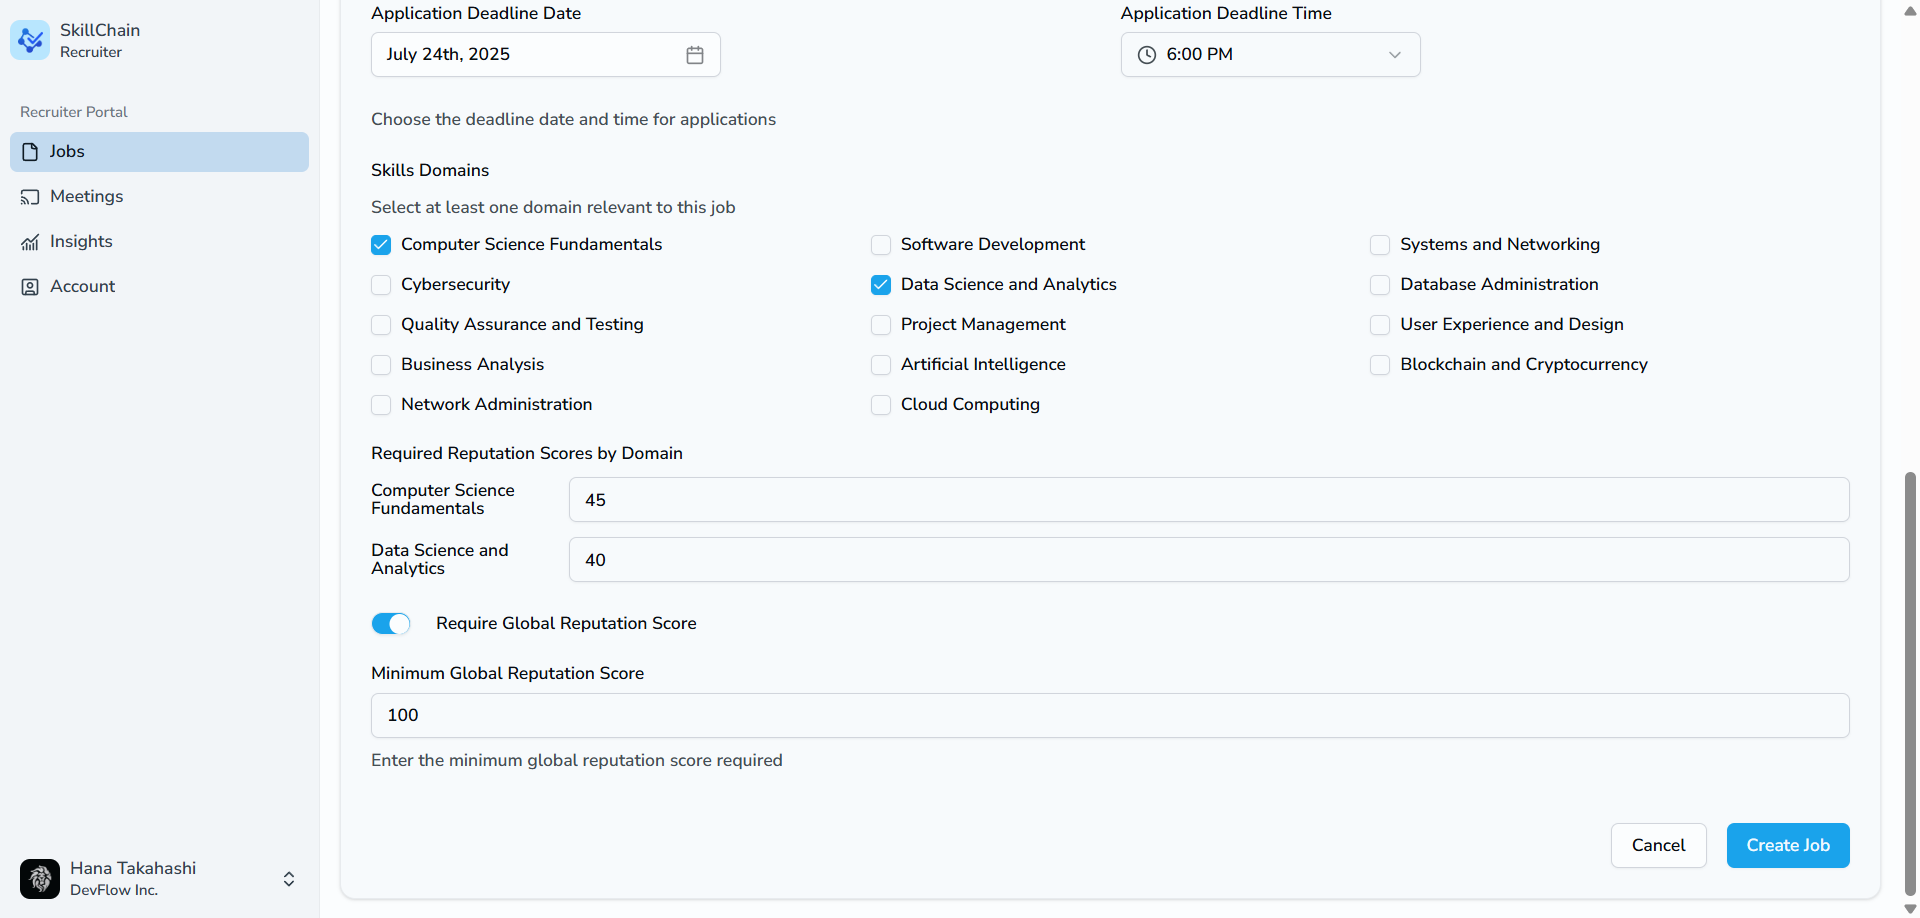
\includegraphics[width=0.99\textwidth, frame]{ui/job-reputation-requirement.png}
  \caption{Yêu cầu uy tín đối với ứng viên}
  \label{fig:job-reputation-requirement}
\end{figure}

\subsubsection{Chỉnh sửa nội dung bài đăng}

Để chỉnh sửa nội dung bài đăng, nhà tuyển dụng có thể thực hiện theo hai cách:
\begin{itemize}
  \item Từ trang chi tiết bài đăng, nhấn ``Edit Job'' ở góc trên bên phải.
  \item Từ danh sách bài đăng, chọn ``Edit job'' tại mục ``Actions''.
\end{itemize}

Hệ thống cho phép chỉnh sửa nội dung trong mọi trạng thái bài đăng mà không phát sinh giao dịch.

\begin{figure}[H]
  \centering
  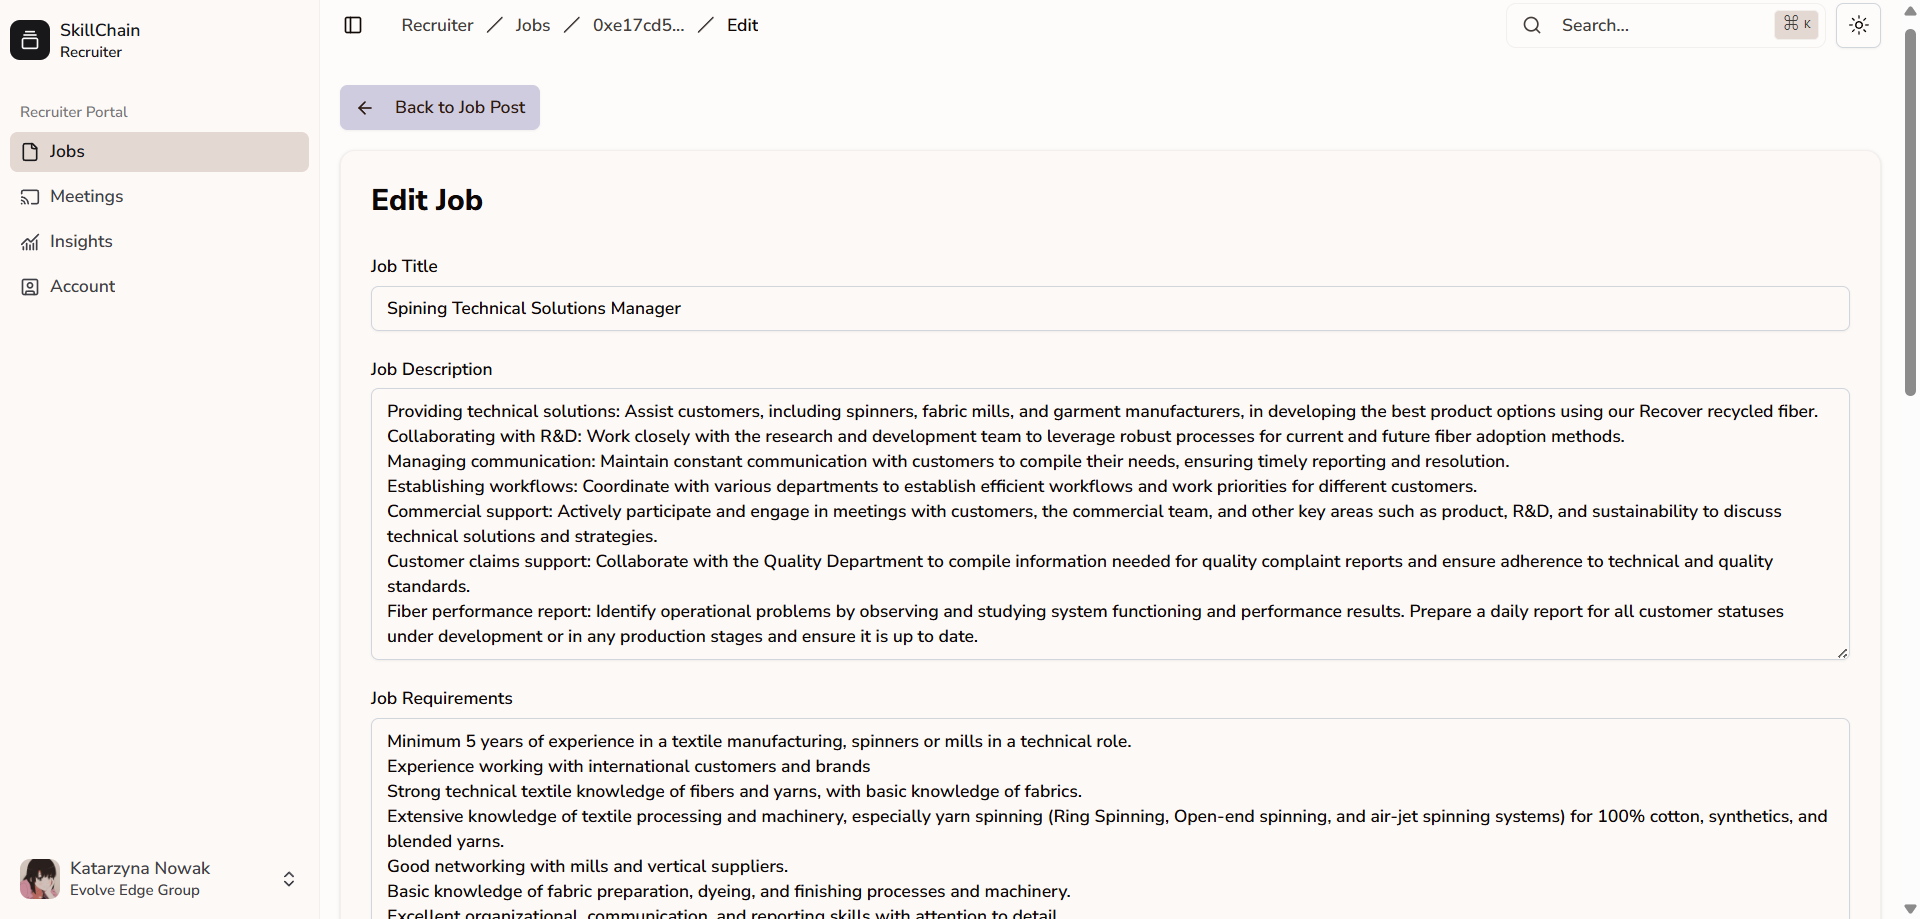
\includegraphics[width=0.99\textwidth, frame]{ui/edit-job-page.png}
  \caption{Trang chỉnh sửa bài đăng tuyển dụng}
  \label{fig:edit-job-page}
\end{figure}

\subsubsection{Chuyển đổi trạng thái bài đăng}

Tại trang chi tiết bài đăng, để thay đổi trạng thái (ví dụ: từ ``nháp'' sang ``đang mở''), nhà tuyển dụng nhấn biểu tượng ba chấm bên cạnh thông tin trạng thái trong phần ``Job Details'' và chọn trạng thái mong muốn.  
Thao tác này yêu cầu xác nhận giao dịch qua ví điện tử.

\subsection{Trang quản lý thông tin ứng tuyển}

\subsubsection{Xem thông tin ứng tuyển}

Để xem danh sách ứng viên đã ứng tuyển cho một bài đăng, nhà tuyển dụng có thể thực hiện theo hai cách:
\begin{itemize}
  \item Từ trang chi tiết bài đăng, nhấn nút ``View Applicants'' trong phần ``Job Overview''.
  \item Từ danh sách bài đăng, chọn ``View applicants'' tại mục ``Actions'' hoặc nhấn vào liên kết tại cột ``Applicants''.
\end{itemize}

\begin{figure}[H]
  \centering
  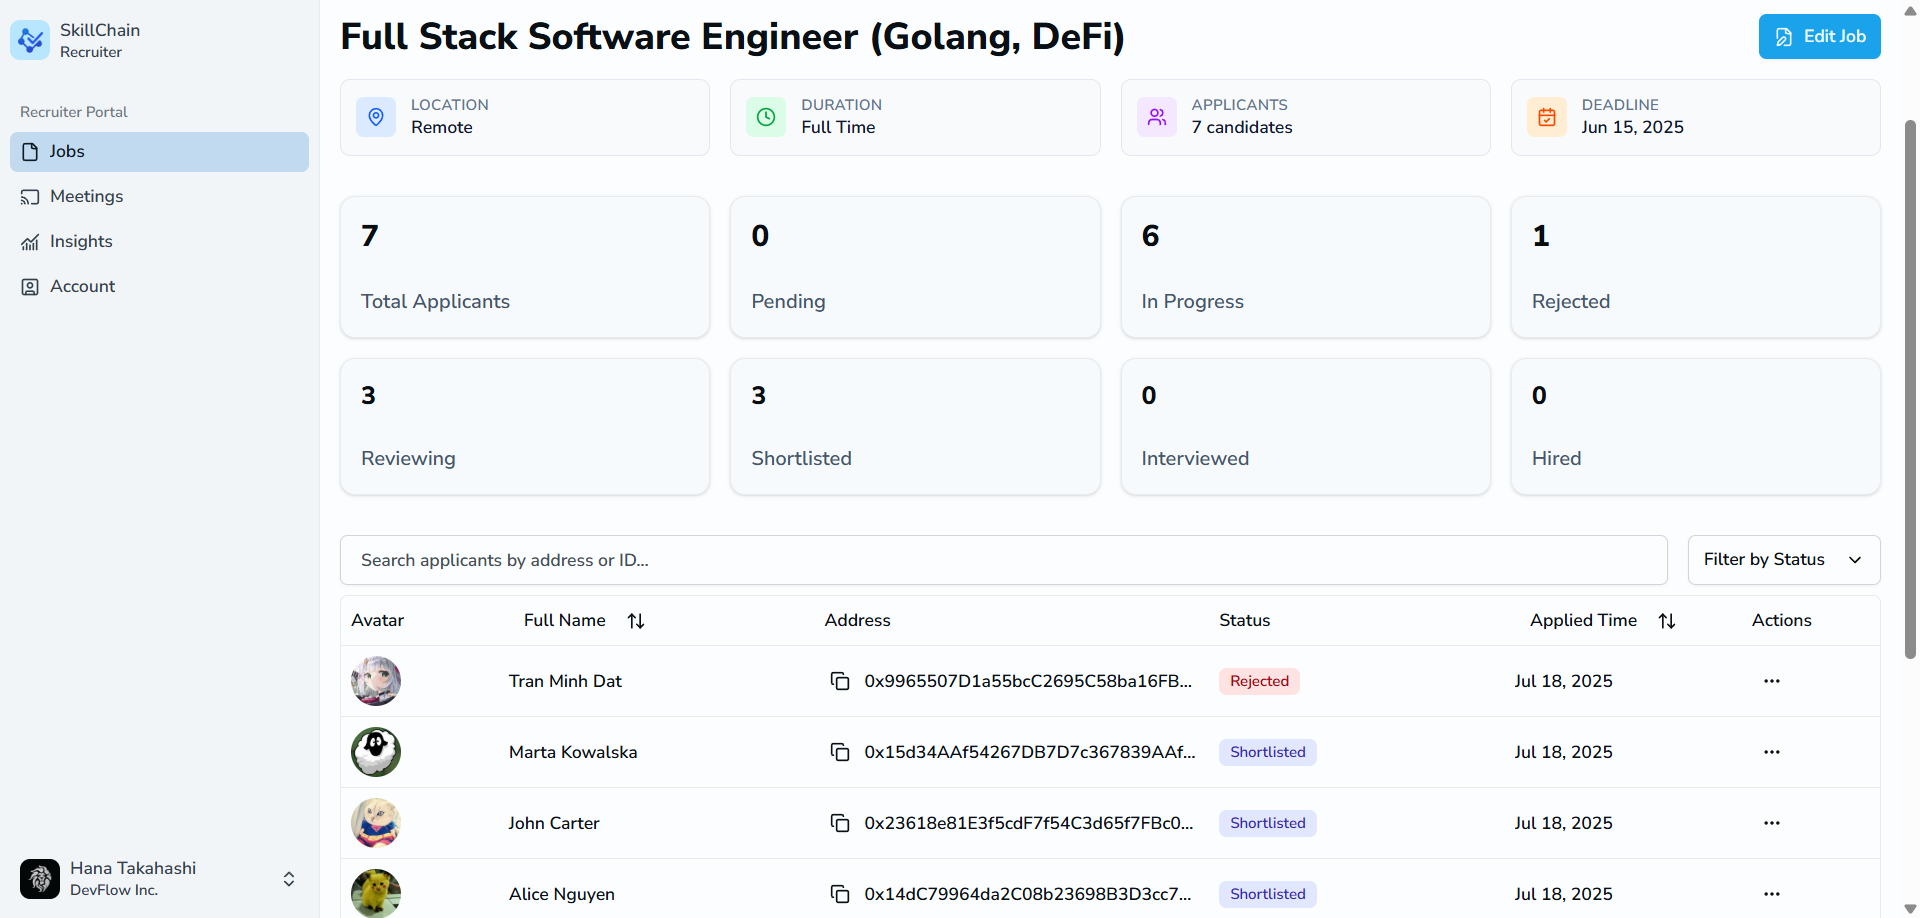
\includegraphics[width=0.99\textwidth, frame]{ui/job-applicants-list-page.png}
  \caption{Danh sách ứng viên ứng tuyển cho một bài đăng}
  \label{fig:job-applicants-list-page}
\end{figure}

Để xem chi tiết hồ sơ một ứng viên, nhà tuyển dụng nhấn ``View application'' tại mục ``Actions'' tương ứng trong danh sách.

\begin{figure}[H]
  \centering
  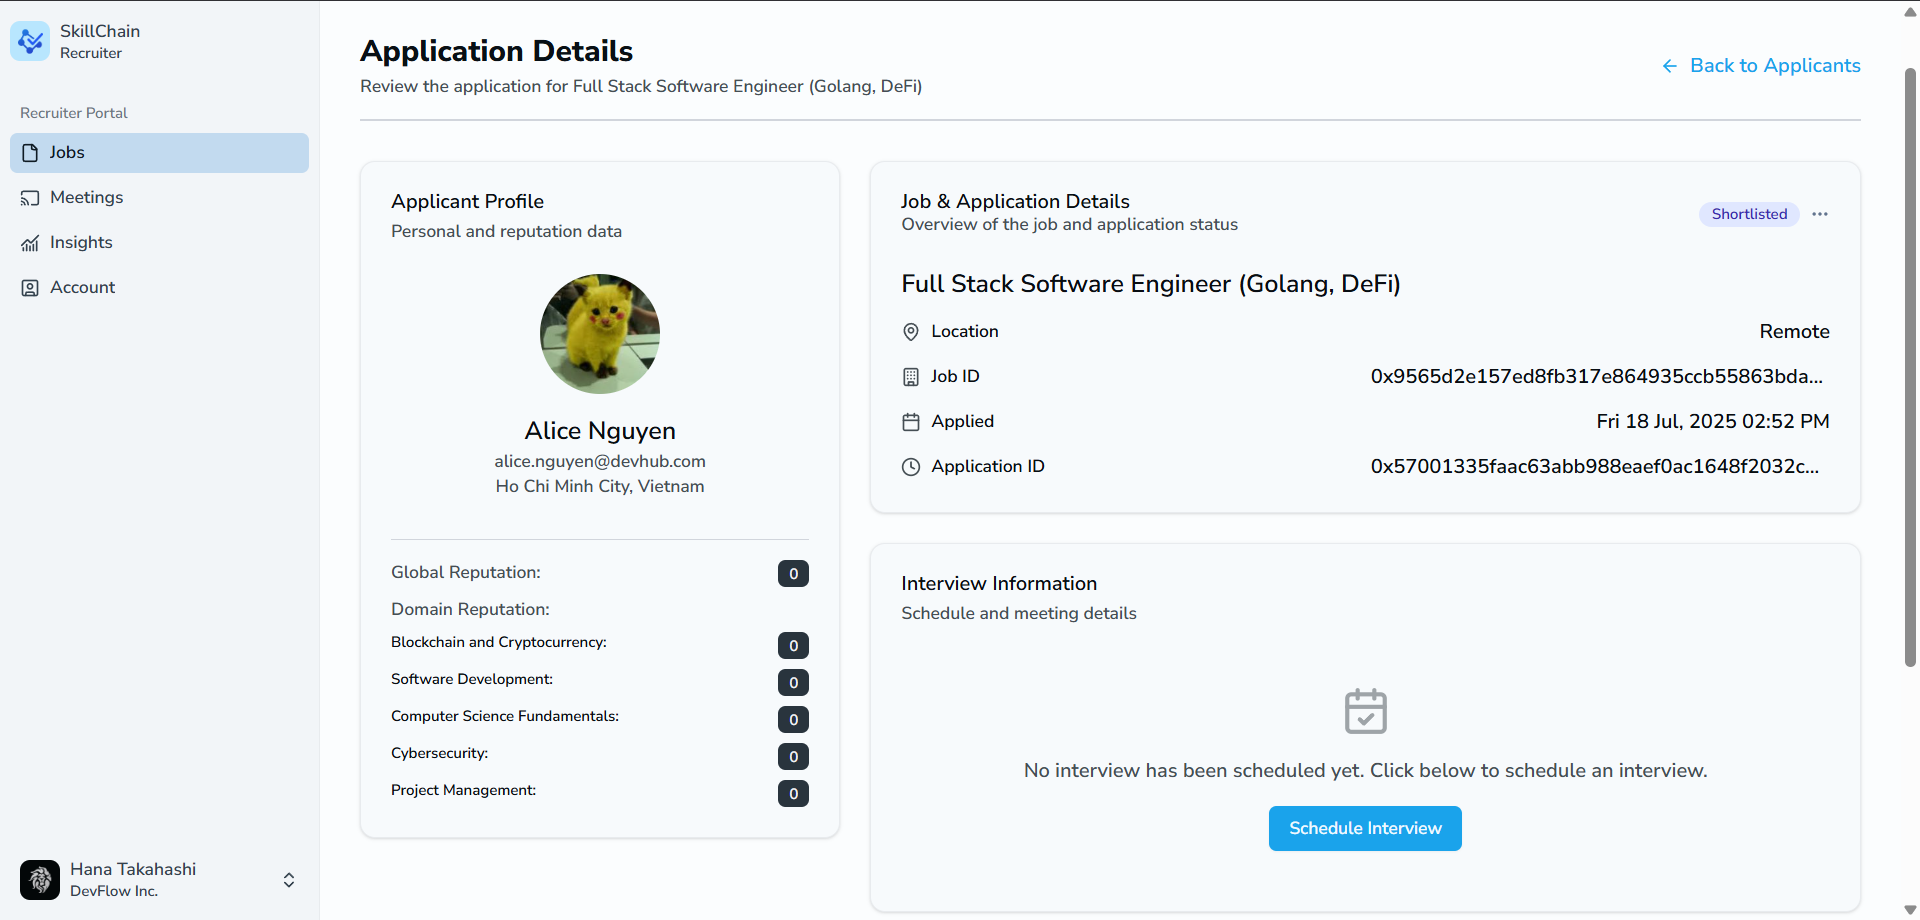
\includegraphics[width=0.99\textwidth, frame]{ui/job-applicant-detail-page.png}
  \caption{Trang chi tiết hồ sơ ứng viên}
  \label{fig:job-applicant-detail-page}
\end{figure}

\subsubsection{Chuyển đổi trạng thái ứng viên}

Tại trang chi tiết hồ sơ ứng viên, để thay đổi trạng thái (ví dụ: từ ``đã đánh giá'' sang ``được rút gọn''), nhà tuyển dụng nhấn biểu tượng ba chấm kế bên thông tin trạng thái trong phần ``Job \& Application Details'' và chọn trạng thái mong muốn.
Hành vi này cần được xác nhận giao dịch thông qua ví tiền điện tử.

\subsection{Trang quản lý lịch họp trực tuyến}

\subsubsection{Xem danh sách cuộc họp}

Để xem danh sách các cuộc họp đã được lên lịch, nhà tuyển dụng truy cập tab \textbf{Meetings}.  
Tại đây, hệ thống hiển thị danh sách các cuộc họp trực tuyến cùng với các thông tin như trạng thái, vị trí công việc, ứng viên liên quan và thời gian diễn ra.

\begin{figure}[H]
  \centering
  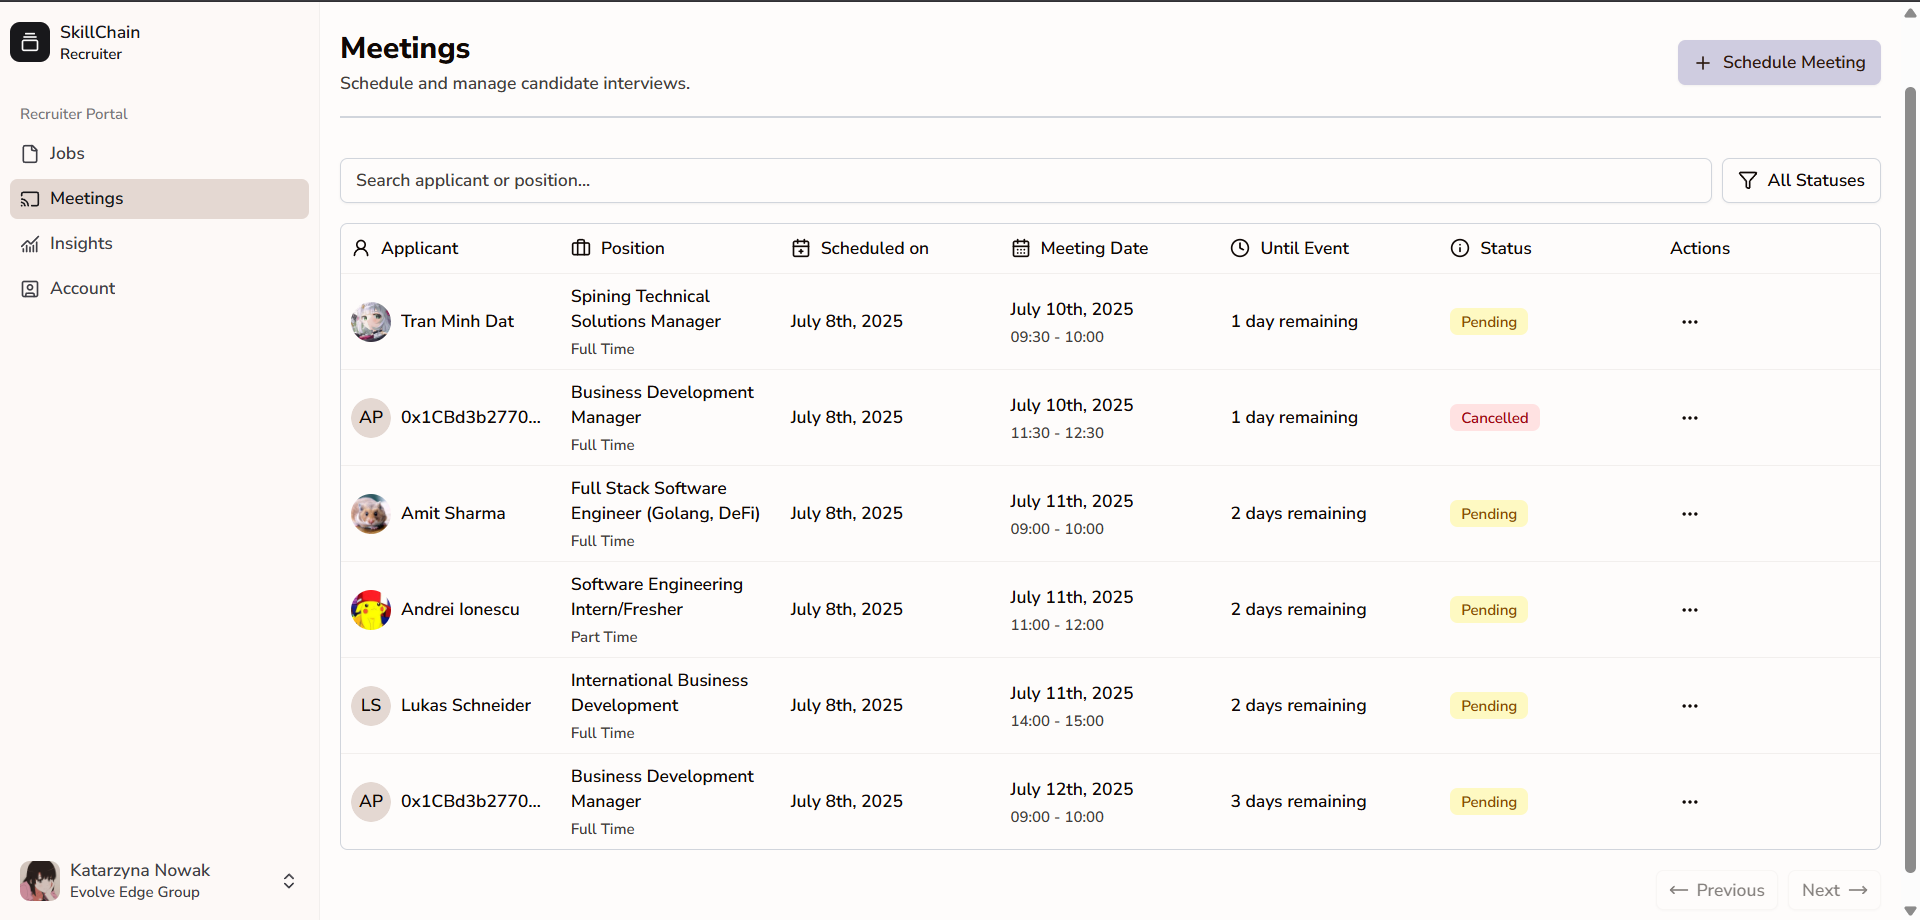
\includegraphics[width=0.99\textwidth, frame]{ui/meeting-list-page.png}
  \caption{Trang danh sách các cuộc họp trực tuyến}
  \label{fig:meeting-list-page}
\end{figure}

Để xem chi tiết một cuộc họp, nhà tuyển dụng nhấn ``View meeting'' tại mục ``Actions'' tương ứng.

\begin{figure}[H]
  \centering
  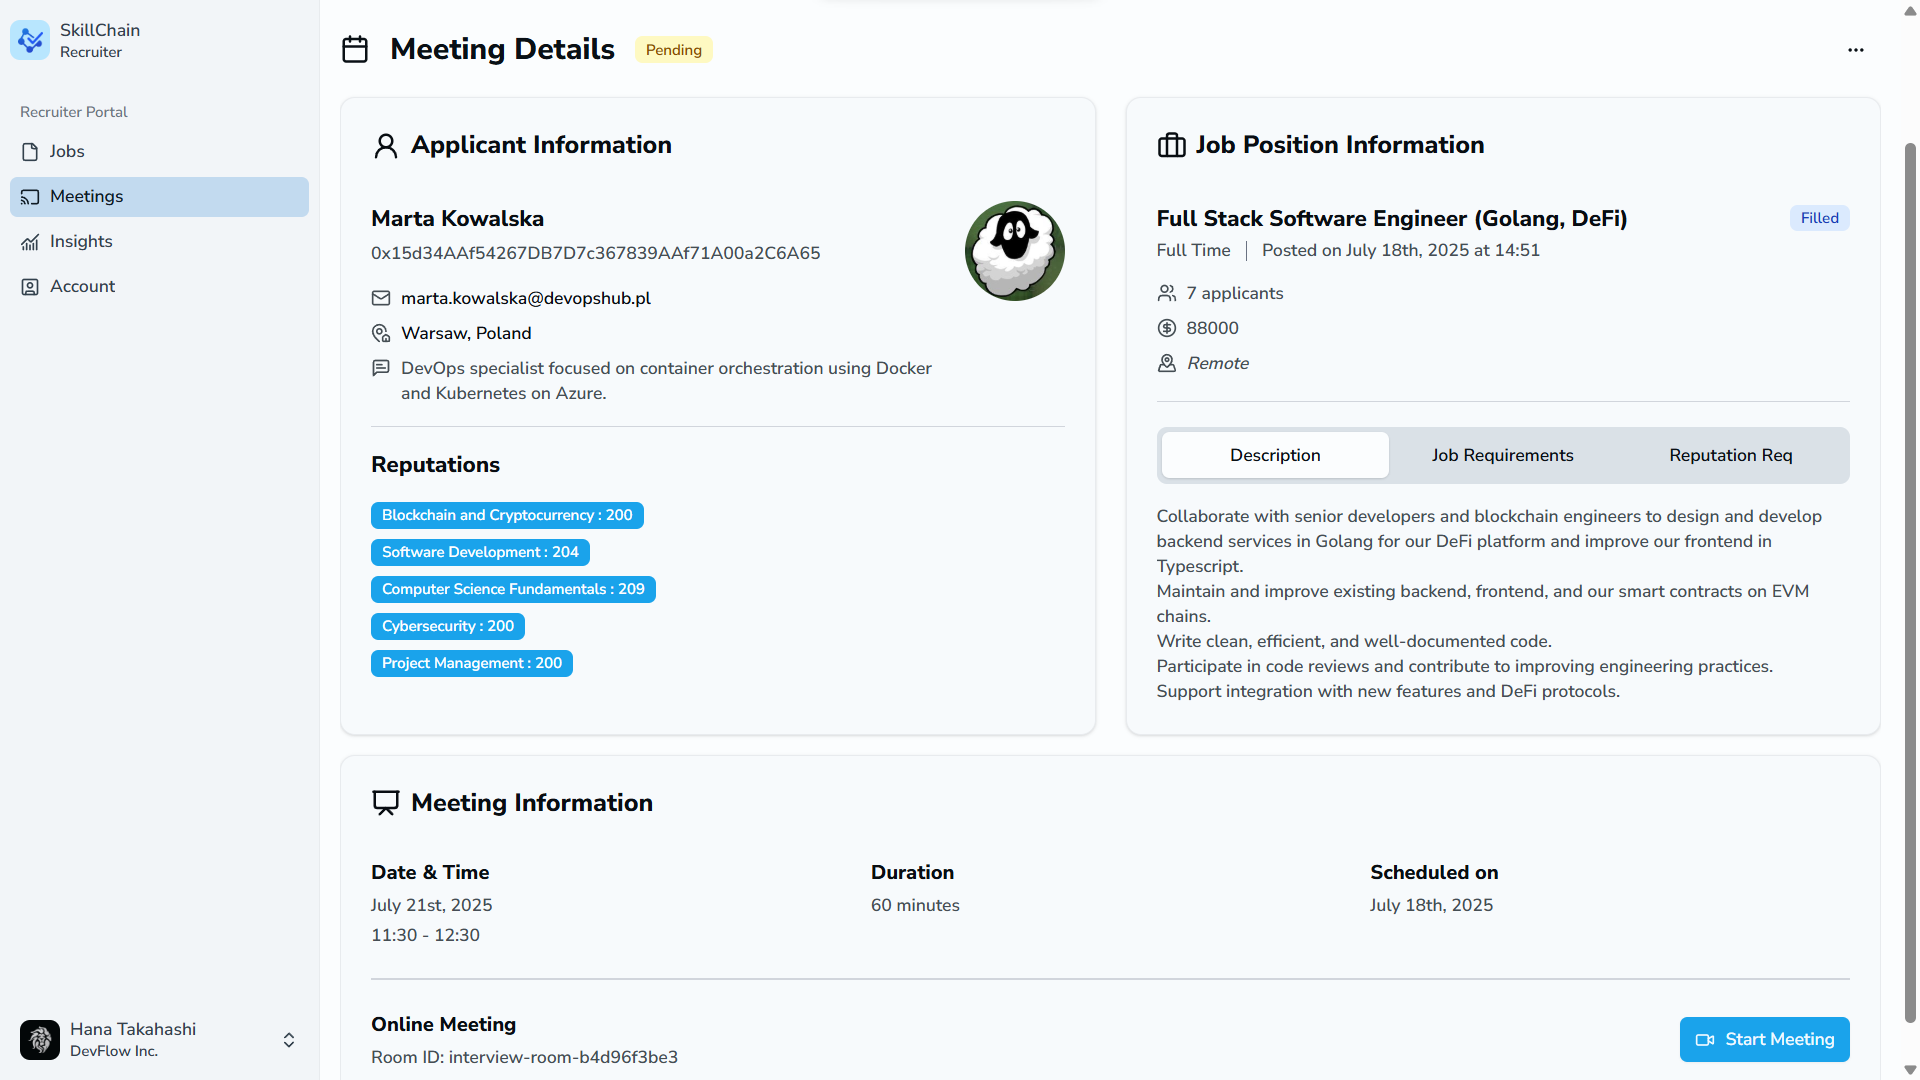
\includegraphics[width=0.99\textwidth, frame]{ui/meeting-detail-page.png}
  \caption{Trang chi tiết một cuộc họp trực tuyến}
  \label{fig:meeting-detail-page}
\end{figure}

Tại trang chi tiết cuộc họp, nhà tuyển dụng có thể đánh dấu trạng thái cuộc họp là \textit{Completed} (Đã hoàn thành) hoặc \textit{Cancelled} (Đã huỷ) bằng cách chọn biểu tượng ba chấm ở góc trên bên phải và thực hiện lựa chọn tương ứng.  
Hành động này yêu cầu xác nhận giao dịch qua ví điện tử.

\subsubsection{Lên lịch một cuộc họp mới}

Để lên lịch một cuộc họp mới, nhà tuyển dụng nhấn nút ``Schedule Meeting'' ở góc trên bên phải trang danh sách cuộc họp.

Tại biểu mẫu lên lịch, nhà tuyển dụng thực hiện các bước:
\begin{enumerate}
  \item Chọn vị trí công việc tương ứng.
  \item Chọn ứng viên thuộc \textbf{danh sách rút gọn} của vị trí đó.
  \item Chọn thời gian diễn ra cuộc họp.
  \item (Tuỳ chọn) Ghi chú gửi đến ứng viên.
\end{enumerate}

Sau khi hoàn tất, nhấn nút ``Schedule'' và xác nhận giao dịch qua ví điện tử để hoàn tất việc lên lịch.

\textbf{Lưu ý:} Nhà tuyển dụng không thể lên lịch một cuộc họp mới cho cùng một ứng viên nếu đã có cuộc họp đang chờ với ứng viên đó.

\begin{figure}[H]
  \centering
  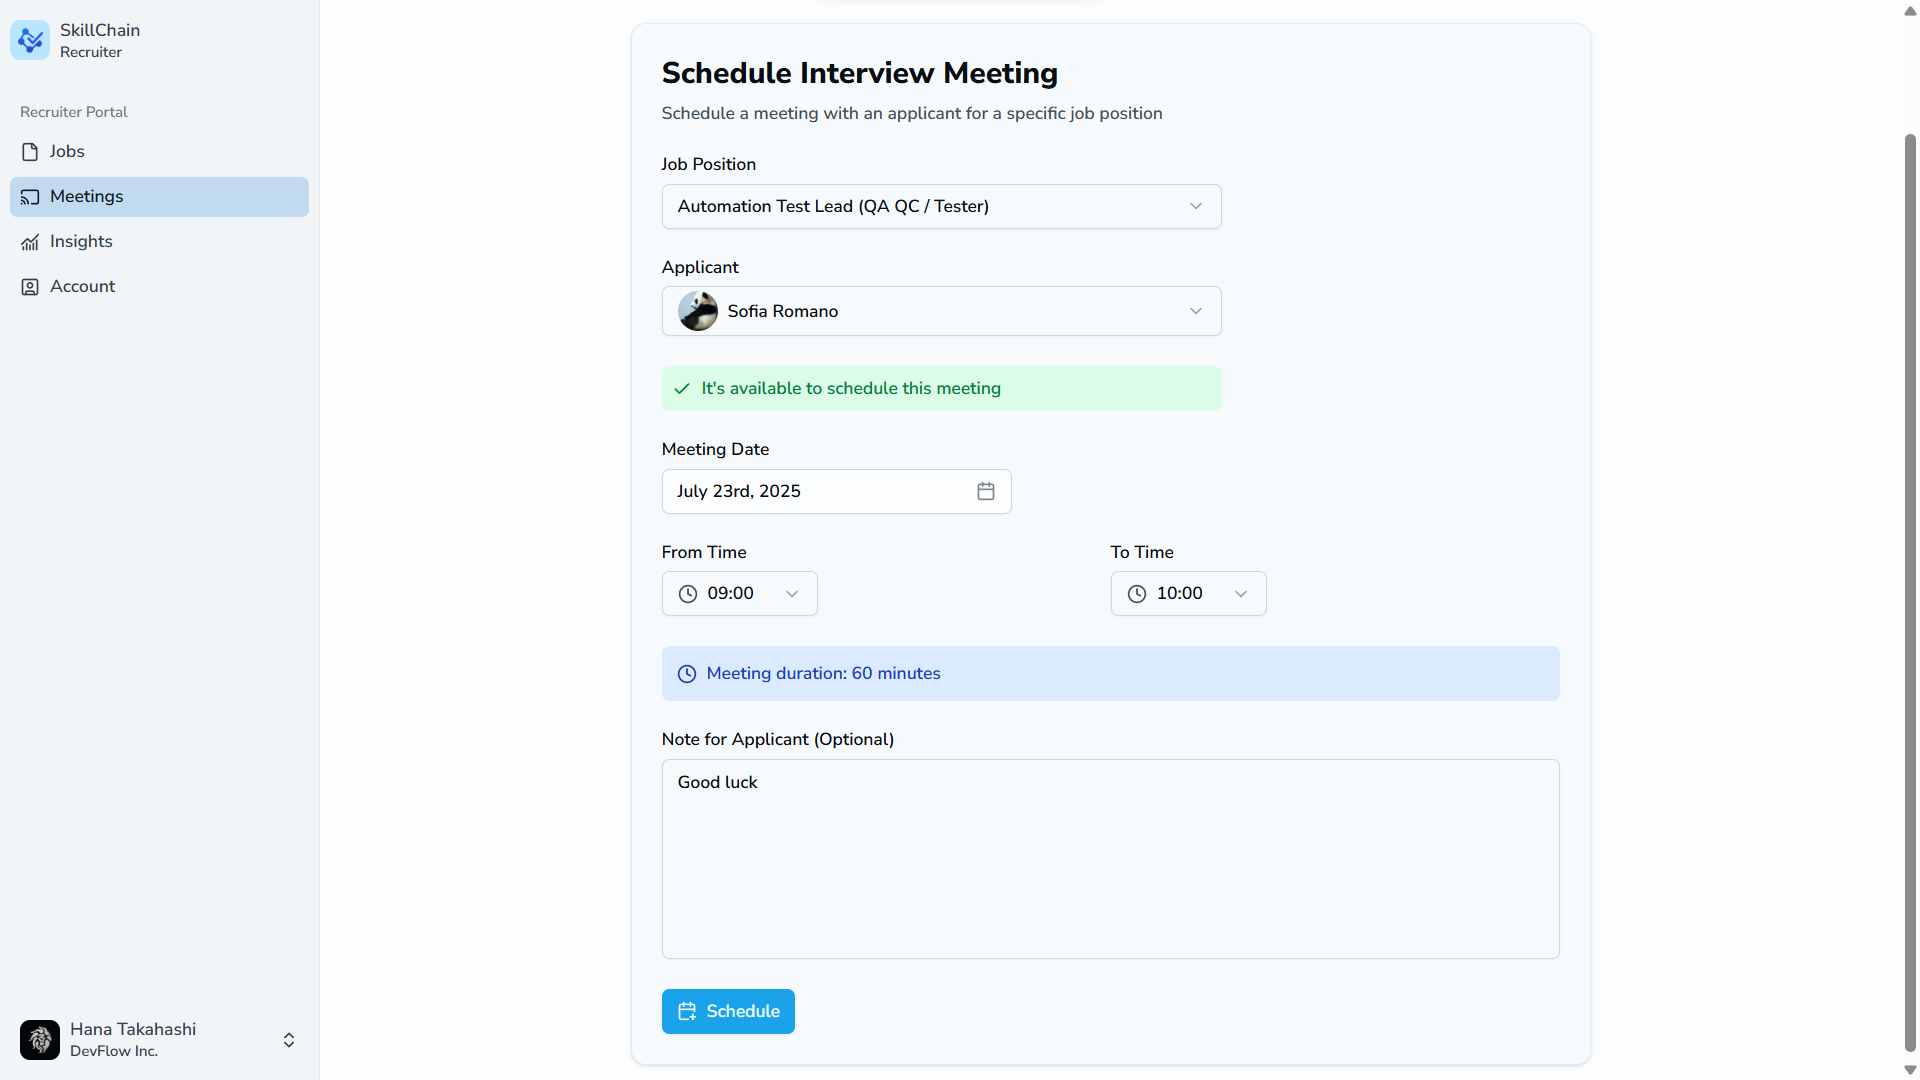
\includegraphics[width=0.99\textwidth, frame]{ui/schedule-meeting-form.png}
  \caption{Biểu mẫu lên lịch cuộc họp}
  \label{fig:schedule-meeting-form}
\end{figure}

\subsubsection{Đổi lịch một cuộc họp}

Đối với các cuộc họp ở trạng thái \textbf{đang chờ}, nhà tuyển dụng có thể thay đổi thời gian họp hoặc ghi chú bằng một trong hai cách:
\begin{itemize}
  \item Từ danh sách cuộc họp, chọn ``Reschedule'' tại mục ``Actions''.
  \item Từ trang chi tiết cuộc họp, nhấn ``Reschedule'' tại biểu tượng ba chấm ở góc trên bên phải.
\end{itemize}

\textbf{Lưu ý:} Không thể thay đổi vị trí công việc hoặc ứng viên đã được chọn.

\begin{figure}[H]
  \centering
  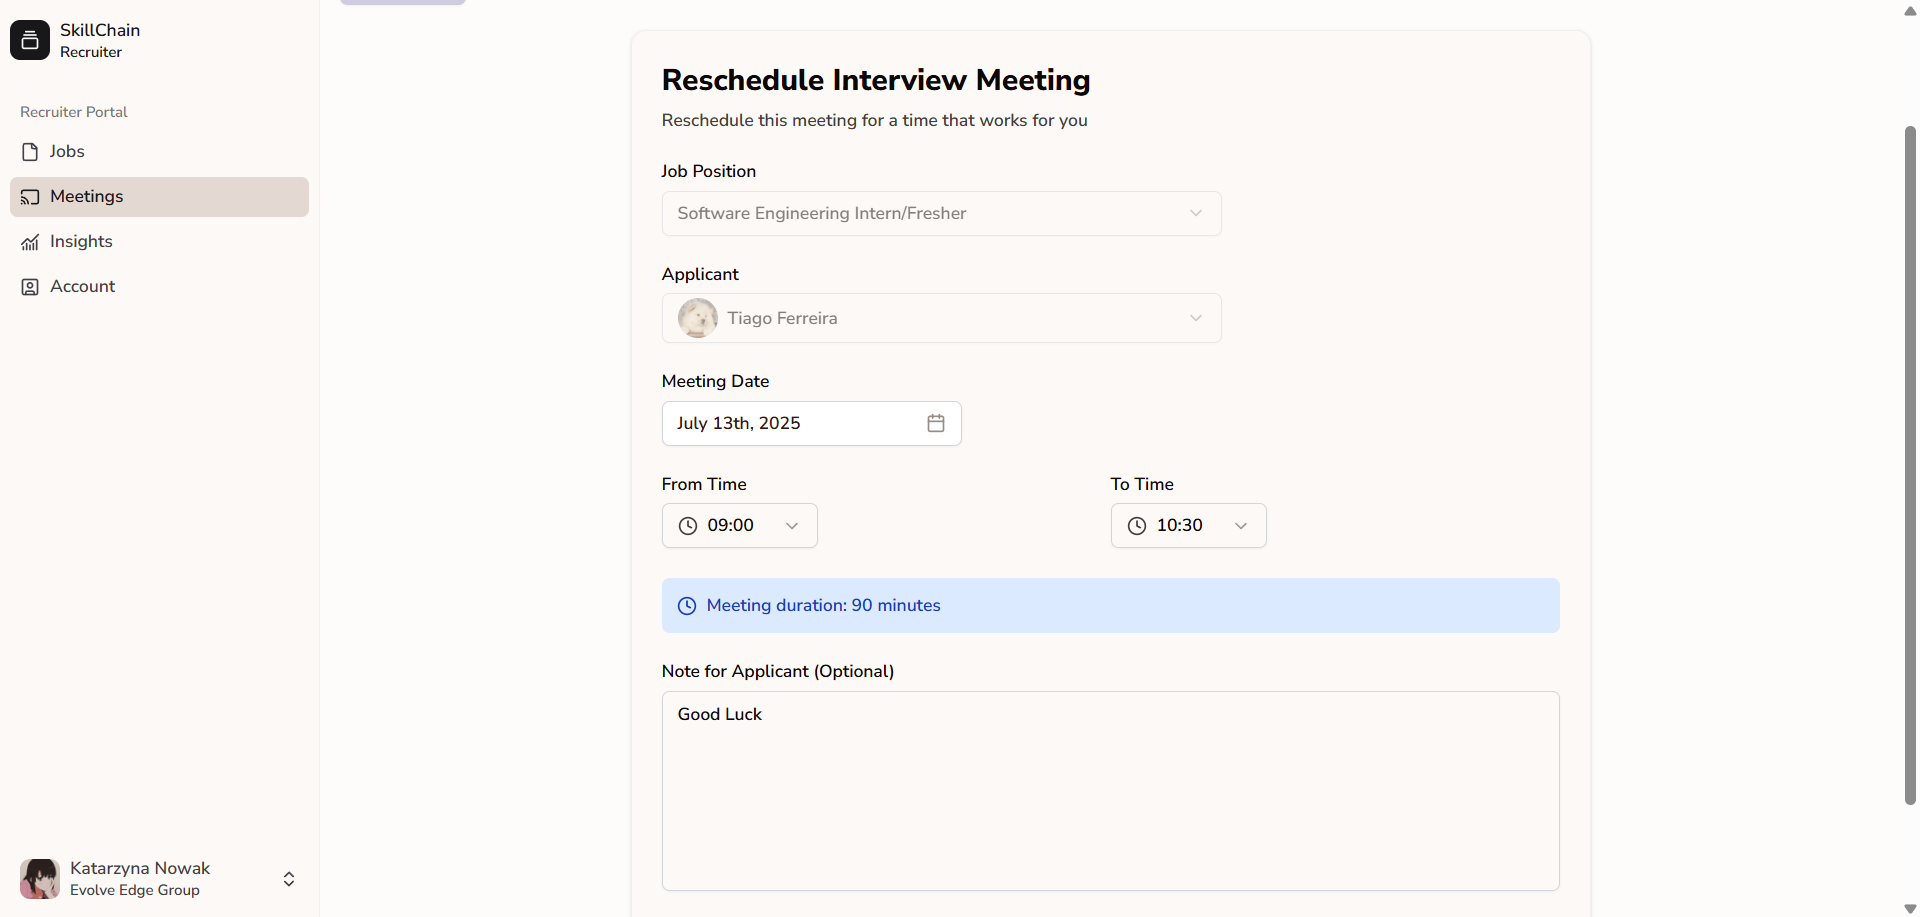
\includegraphics[width=0.99\textwidth, frame]{ui/reschedule-meeting-form.png}
  \caption{Biểu mẫu thay đổi lịch họp}
  \label{fig:reschedule-meeting-form}
\end{figure}

\subsubsection{Triển khai cuộc họp}

Khi đến thời điểm họp, tại trang chi tiết cuộc họp, nhà tuyển dụng nhấn nút ``Start Meeting'' để tạo và khởi chạy phòng họp trực tuyến.  
Hệ thống sẽ tạo liên kết tham gia và gửi đến ứng viên tương ứng.

\begin{figure}[H]
  \centering
  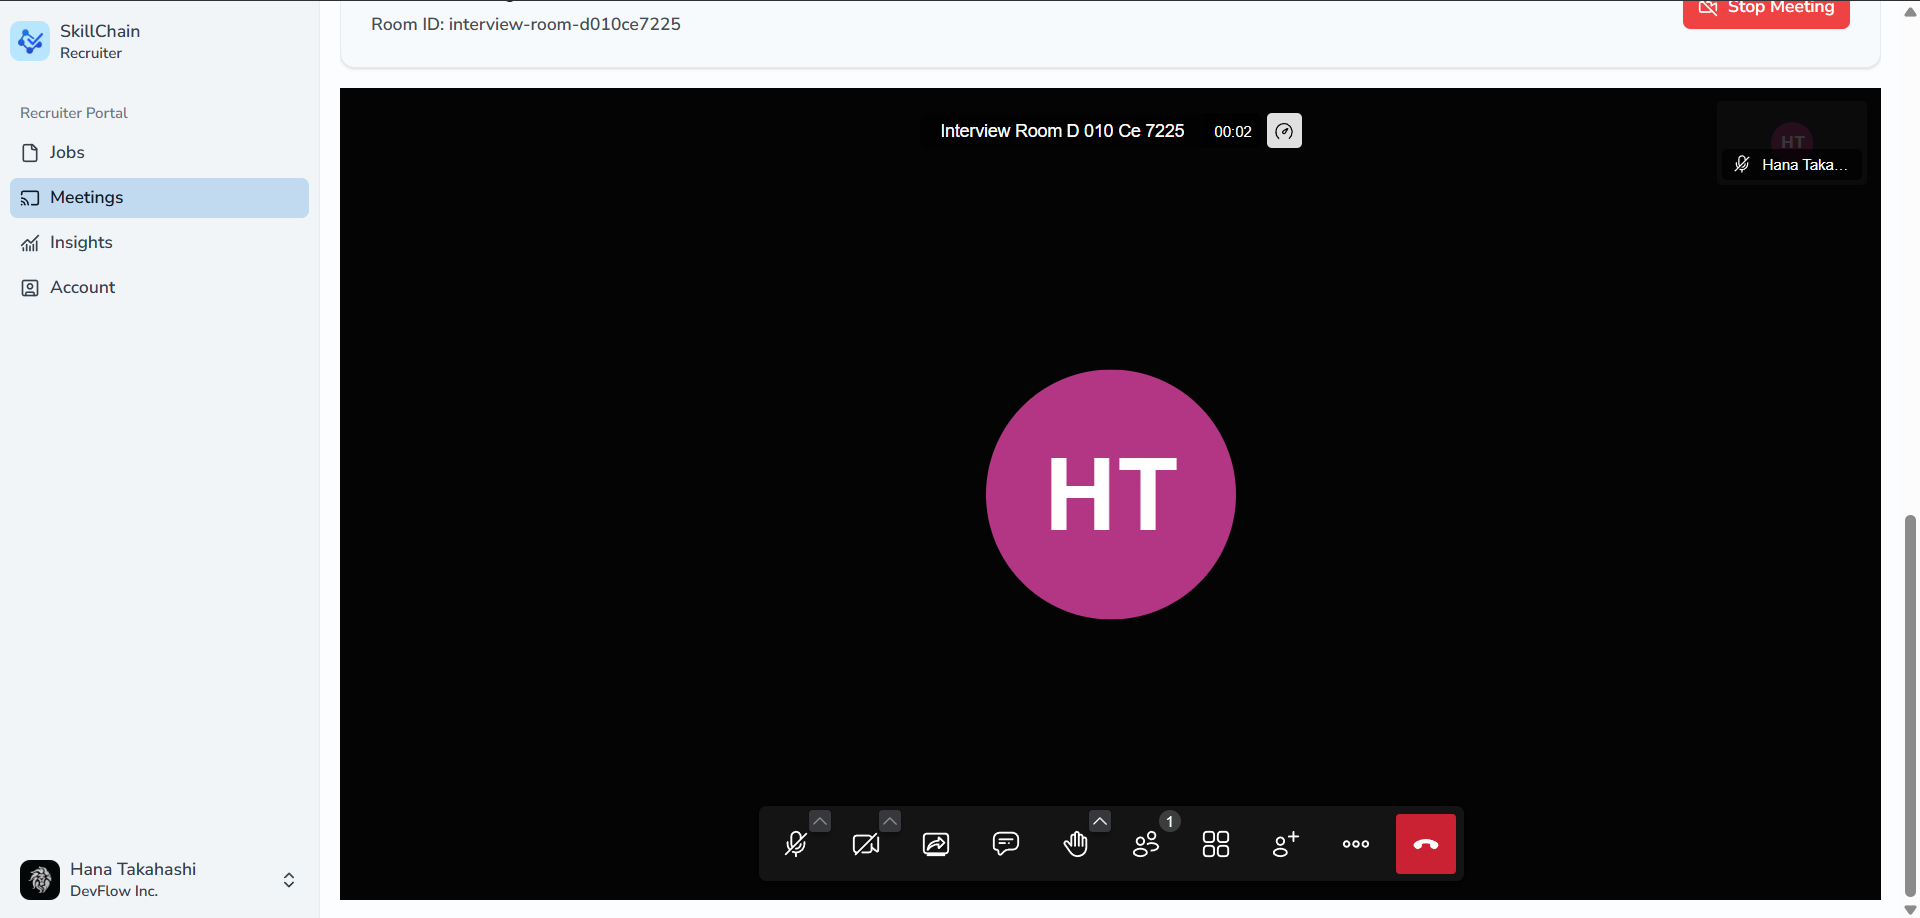
\includegraphics[width=0.99\textwidth, frame]{ui/meeting-hosting.png}
  \caption{Khởi chạy phòng họp trực tuyến}
  \label{fig:meeting-hosting}
\end{figure}

\subsection{Trang số liệu thống kê}

Để xem các số liệu thống kê liên quan đến quá trình tuyển dụng, nhà tuyển dụng truy cập tab \textbf{Insights}.  
Tại đây, hệ thống hiển thị các chỉ số tổng quan giúp đánh giá hiệu quả hoạt động tuyển dụng.
Bốn chỉ số mặc định được hiển thị gồm:
\begin{itemize}
  \item \textbf{Active Jobs}: Số lượng bài đăng tuyển dụng đang hoạt động.
  \item \textbf{Total Applicants}: Tổng số lượng ứng viên đã ứng tuyển.
  \item \textbf{Conversion Rate}: Tỷ lệ chuyển đổi từ ứng tuyển sang đã tuyển.
  \item \textbf{Pending Meetings}: Số lượng cuộc họp đang chờ diễn ra.
\end{itemize}

\begin{figure}[H]
  \centering
  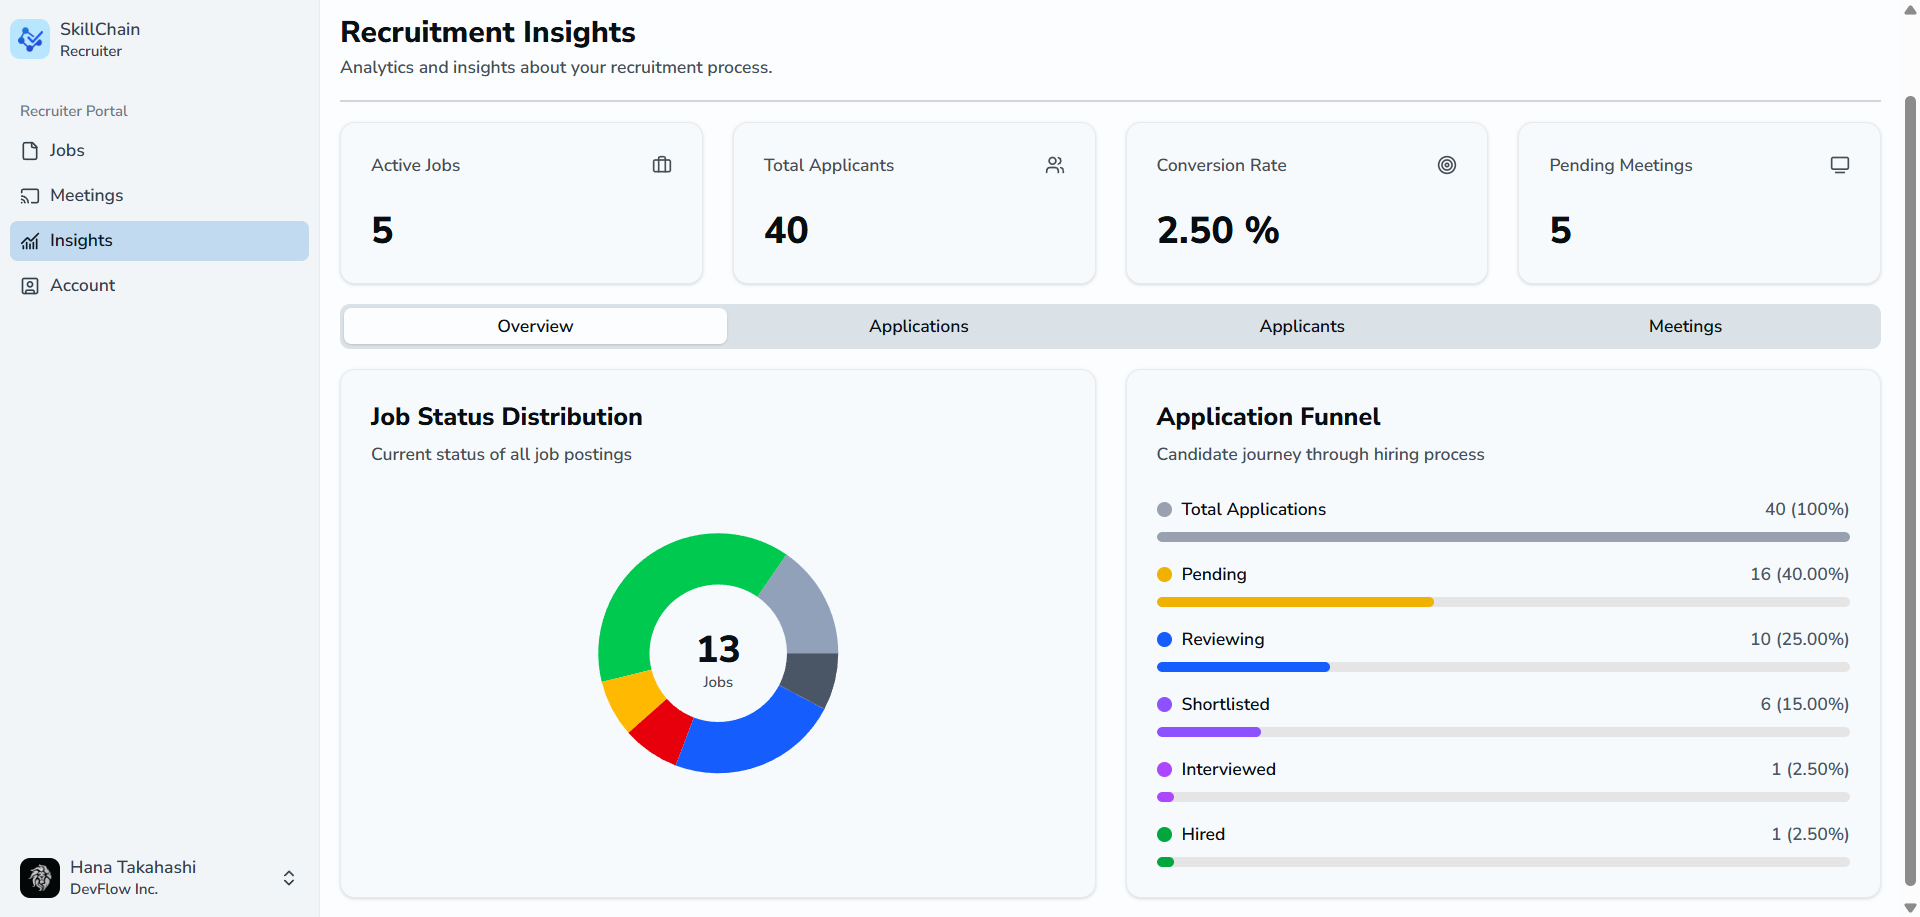
\includegraphics[width=0.99\textwidth, frame]{ui/recruiment-insight-page.png}
  \caption{Trang thống kê quá trình tuyển dụng}
  \label{fig:recruiment-insight-page}
\end{figure}

\subsubsection{Tab tổng quan (Overview)}

Tab \textbf{Overview} hiển thị hai biểu đồ trực quan:
\begin{itemize}
  \item \textbf{Job Status Distribution}: Biểu đồ tròn thể hiện số lượng các trạng thái bài đăng tuyển dụng (đang mở, đã đóng, nháp, v.v.).
  \item \textbf{Application Funnel}: Biểu đồ hình phễu mô tả tỷ lệ và số lượng ứng viên ở một số giai đoạn trong quy trình tuyển dụng.
\end{itemize}

\subsubsection{Tab ứng tuyển (Applications)}

Tab \textbf{Applications} hiển thị danh sách \textbf{Top 5 công việc có hiệu suất tốt nhất}, dựa trên:
\begin{itemize}
  \item Số lượng ứng viên ứng tuyển.
  \item Tỷ lệ chuyển đổi từ ứng viên sang đã tuyển dụng.
\end{itemize}

\begin{figure}[H]
  \centering
  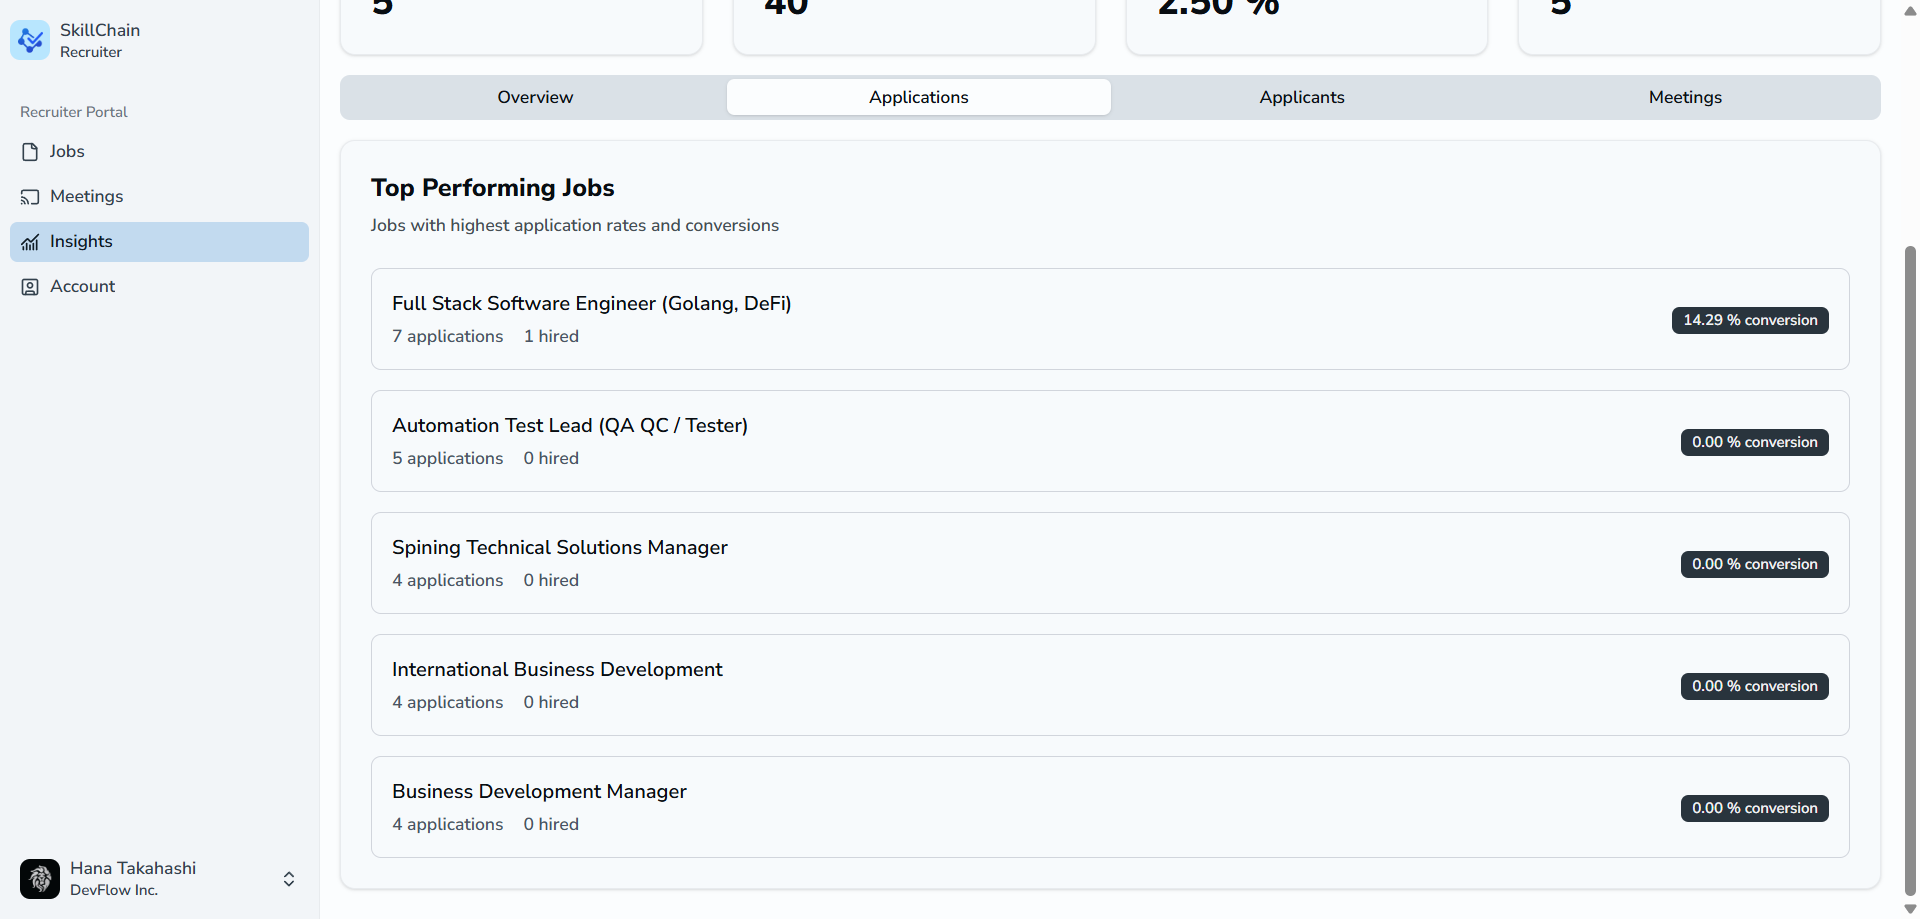
\includegraphics[width=0.99\textwidth, frame]{ui/top-performing-jobs.png}
  \caption{Năm công việc có hiệu suất tuyển dụng cao nhất}
  \label{fig:top-performing-jobs}
\end{figure}

\subsubsection{Tab ứng viên (Applicants)}

Tab \textbf{Applicants} hiển thị \textbf{Top 5 ứng viên tương tác nhiều nhất}, được đánh giá dựa trên số lượng bài đăng từ nhà tuyển dụng mà họ đã ứng tuyển.

\begin{figure}[H]
  \centering
  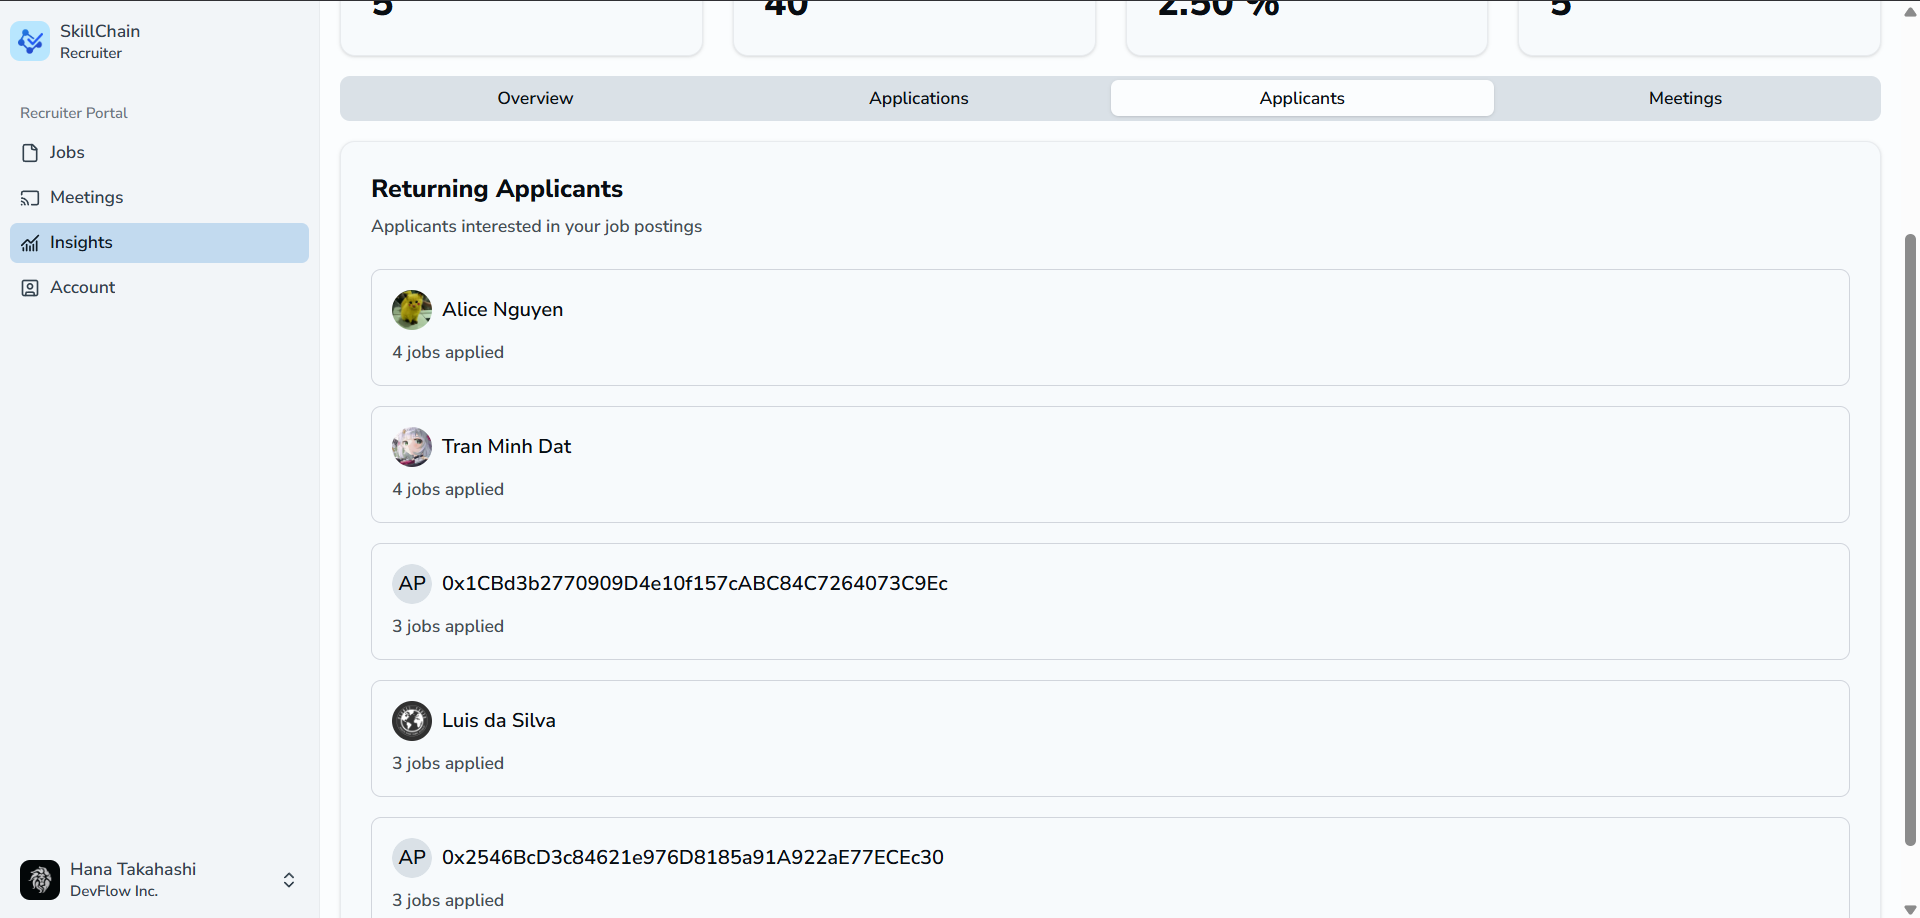
\includegraphics[width=0.99\textwidth, frame]{ui/top-returning-applicants.png}
  \caption{Năm ứng viên tương tác nhiều nhất với nhà tuyển dụng}
  \label{fig:top-returning-applicants}
\end{figure}

\subsubsection{Tab cuộc họp (Meetings)}

Tab \textbf{Meetings} cung cấp:
\begin{itemize}
  \item \textbf{Meeting Status Distribution}: Biểu đồ phân bố trạng thái các cuộc họp (đã hoàn thành, đang chờ, đã huỷ).
  \item \textbf{Upcoming Meetings}: Danh sách những cuộc họp sắp diễn ra, giúp nhà tuyển dụng chủ động chuẩn bị.
\end{itemize}

\begin{figure}[H]
  \centering
  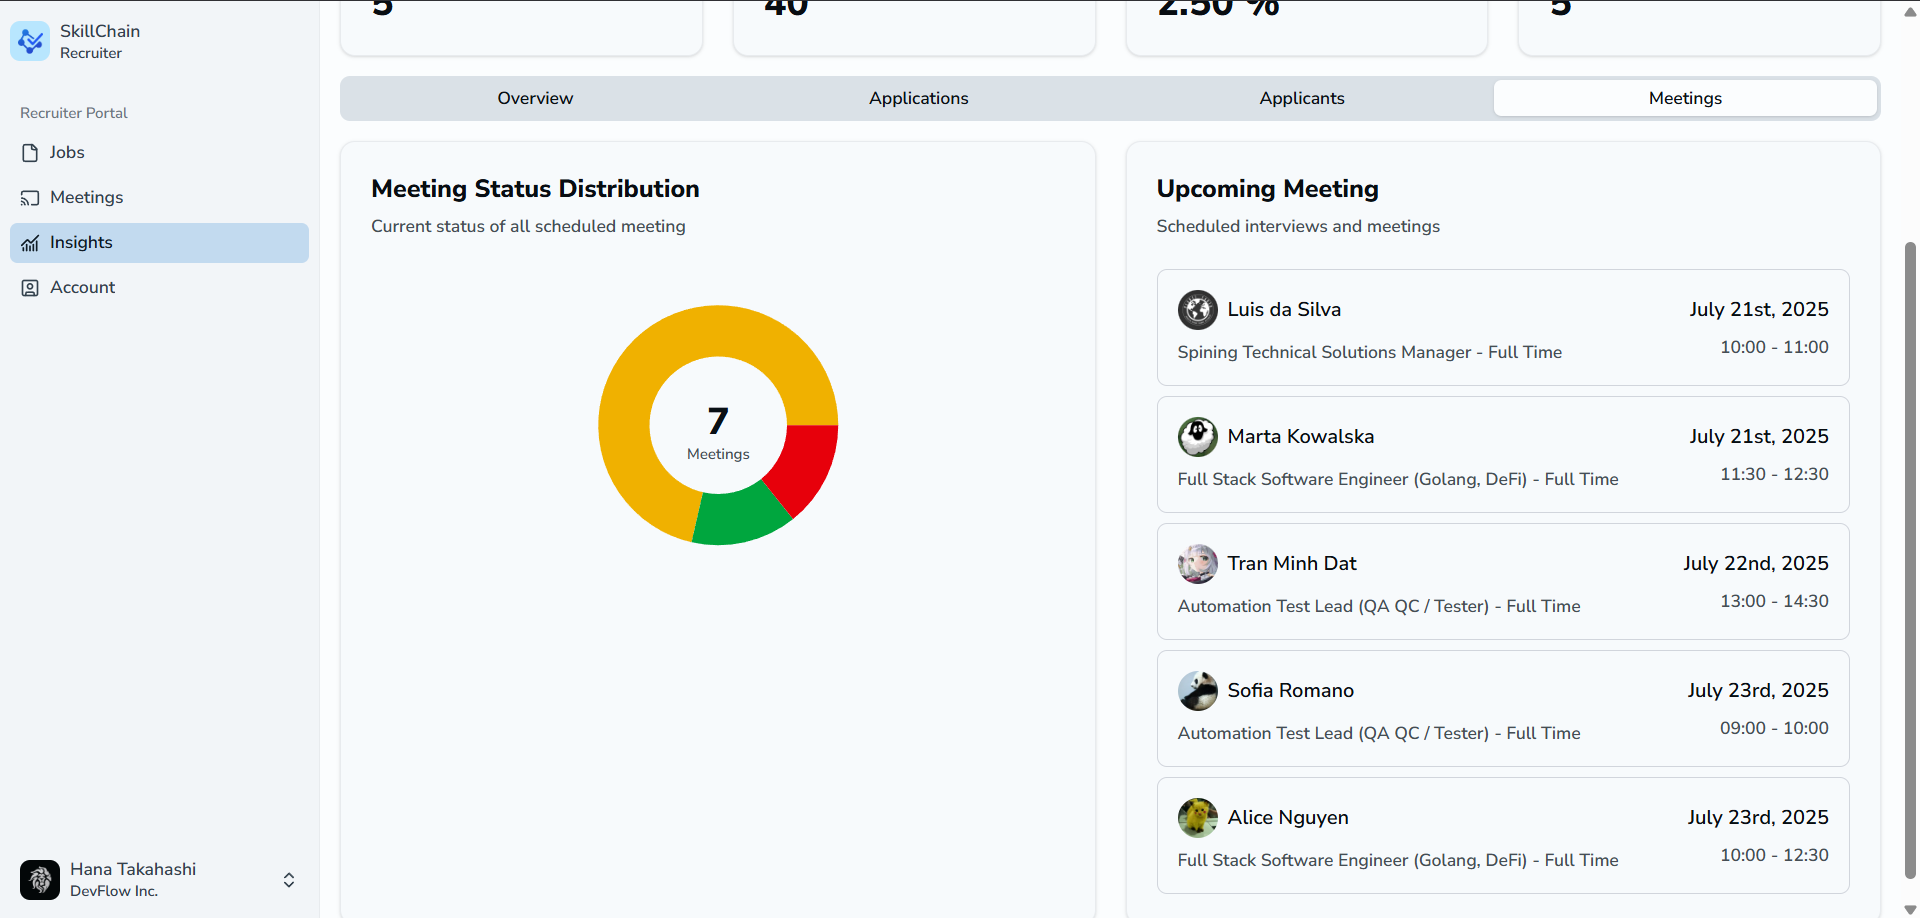
\includegraphics[width=0.99\textwidth, frame]{ui/insight-meetings-tab.png}
  \caption{Thống kê về các cuộc họp phỏng vấn}
  \label{fig:insight-meetings-tab}
\end{figure}

\subsection{Trang người dùng tham gia ứng tuyển}

\subsubsection{Xem danh sách công việc đang mở}

Để xem danh sách các công việc đang tuyển dụng, người dùng truy cập \textbf{Career} $\rightarrow$ \textbf{Available Jobs} trong không gian xây dựng uy tín.

\begin{figure}[H]
  \centering
  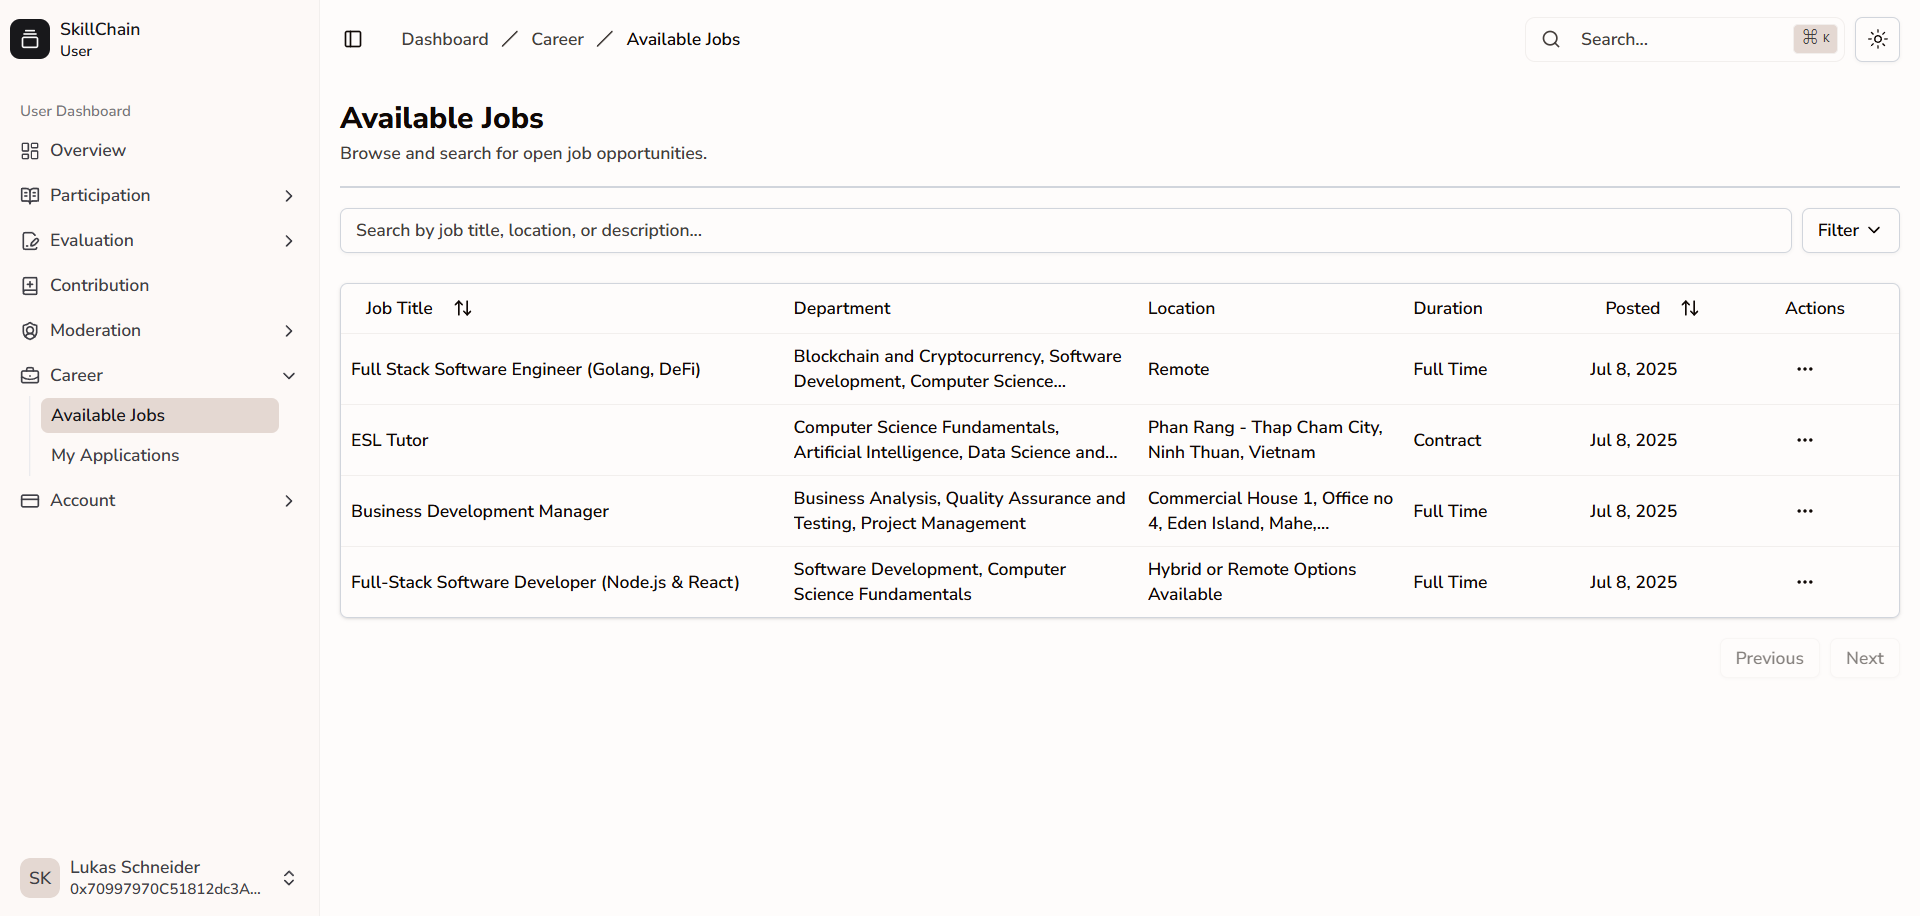
\includegraphics[width=0.99\textwidth, frame]{ui/available-jobs-page.png}
  \caption{Trang các công việc đang mở}
  \label{fig:available-jobs-page}
\end{figure}

Tại đây, người dùng có thể xem thông tin cơ bản của từng công việc như vị trí tuyển dụng, yêu cầu uy tín hay thời gian làm việc. 
Để xem chi tiết, nhấn nút ``View job'' tại mục ``Actions'' tương ứng.

\begin{figure}[H]
  \centering
  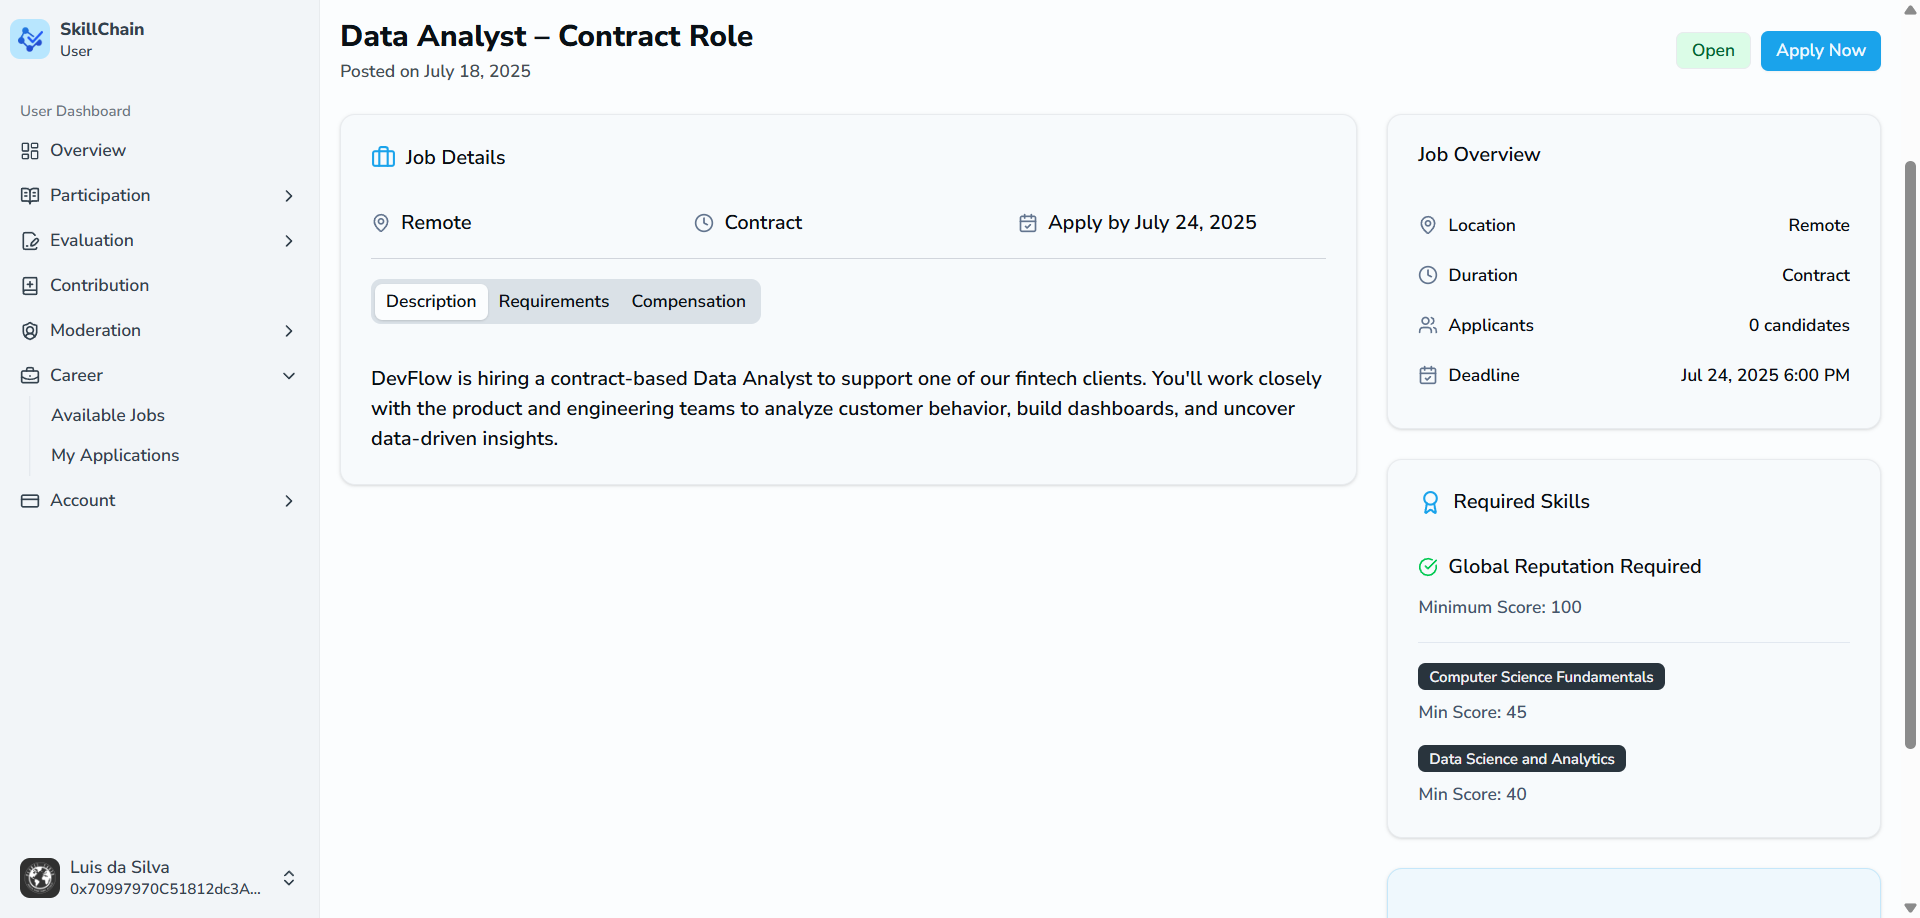
\includegraphics[width=0.99\textwidth, frame]{ui/available-job-detail-page.png}
  \caption{Trang chi tiết một công việc}
  \label{fig:available-job-detail-page}
\end{figure}

\subsubsection{Tham gia ứng tuyển}

Khi truy cập trang chi tiết công việc, hệ thống sẽ tự động kiểm tra mức độ uy tín của người dùng. Nếu không đáp ứng yêu cầu, hệ thống sẽ hiển thị thông báo và vô hiệu hóa nút ứng tuyển. 
Nếu đủ điều kiện, người dùng có thể nhấn nút ``Apply'' ở góc trên bên phải để nộp đơn ứng tuyển. Hành vi này yêu cầu xác nhận giao dịch thông qua ví tiền điện tử.

\subsubsection{Xem các công việc đã ứng tuyển}

Để theo dõi các công việc đã ứng tuyển, người dùng truy cập \textbf{Career} $\rightarrow$ \textbf{My Applications}. Tại đây, hệ thống hiển thị danh sách các công việc mà người dùng đã nộp đơn cùng với trạng thái tương ứng.

\begin{figure}[H]
  \centering
  \includegraphics[width=0.99\textwidth, frame]{ui/my-applications-page.png}
  \caption{Trang công việc đã ứng tuyển}
  \label{fig:my-applications-page}
\end{figure}

Để xem thông tin chi tiết của một đơn ứng tuyển, nhấn ``View application'' tại nút ``Actions'' của công việc tương ứng. 
Trong trường hợp người dùng được đưa vào danh sách rút gọn, hệ thống sẽ hiển thị thêm thông tin lịch họp và liên kết tham gia phòng họp trực tuyến (nếu nhà tuyển dụng đã lên lịch).

\begin{figure}[H]
  \centering
  \includegraphics[width=0.99\textwidth, frame]{ui/my-application-detail-page.png}
  \caption{Trang chi tiết của một đơn ứng tuyển}
  \label{fig:my-application-detail-page}
\end{figure}

\subsubsection{Rút đơn ứng tuyển}

Nếu người dùng muốn hủy ứng tuyển, có thể nhấn nút ``Withdraw Application'' ở góc trên bên phải tại trang chi tiết ứng tuyển. Hành vi này yêu cầu xác nhận giao dịch thông qua ví tiền điện tử.
Người dùng sau đó sẽ không thể ứng tuyển lại cho vị trí này nữa.

\chapter{Kết quả đạt được}

\section{Các chức năng chính đã hoàn thiện}
\subsection{Chức năng cho người dùng}

Chúng tôi đã phát triển thành công các chức năng sau dành cho \textbf{người dùng phổ thông} (bao gồm người học, người đóng góp, người kiểm duyệt và người đánh giá):

\begin{itemize}
  \item Kết nối ví người dùng với hệ thống.
  \item Đăng ký thông tin cá nhân khi lần đầu kết nối.
  \item Xem và cập nhật thông tin cá nhân.
  \item Truy cập hồ sơ uy tín, bao gồm uy tín toàn cục và uy tín chuyên môn theo từng lĩnh vực.
  \item Theo dõi vai trò hiện có của bản thân trong từng lĩnh vực chuyên môn.
  \item Duyệt danh sách các thử thách đang hoạt động trên hệ thống.
  \item Tham gia thử thách nếu đáp ứng yêu cầu về số dư POL.
  \item Xem danh sách thử thách đã và đang tham gia.
  \item Làm việc trên giải pháp thử thách thông qua không gian cá nhân; hỗ trợ chỉnh sửa và lưu trữ tùy ý.
  \item Nộp và gửi giải pháp cho hội đồng đánh giá.
  \item Xem điểm đánh giá cuối cùng và thông tin liên quan sau khi phiên đánh giá kết thúc.
  \item Duyệt danh sách các bài đăng tuyển dụng hiện hành và xem chi tiết từng bài.
  \item Ứng tuyển vào bài đăng tuyển dụng; hệ thống hỗ trợ tính toán khả năng ứng tuyển dựa trên hồ sơ uy tín và yêu cầu từ nhà tuyển dụng.
  \item Xem danh sách các đơn ứng tuyển kèm theo trạng thái; cho phép rút đơn nếu người dùng mong muốn.
  \item Trong trường hợp được đưa vào danh sách rút gọn, người dùng có thể xem thông tin cuộc họp trực tuyến do nhà tuyển dụng tổ chức và tham gia nếu đã được lên lịch.
\end{itemize}

Tiếp theo là các chức năng đặc thù dành cho từng vai trò trong hệ thống:

\subsubsection{Người đóng góp}

\begin{itemize}
  \item Tạo thử thách mới ở trạng thái nháp (chỉ được phép nếu uy tín chuyên môn đủ điều kiện theo lĩnh vực).
  \item Làm việc trên thử thách nháp trong không gian chỉnh sửa cá nhân, có thể lưu lại tùy ý.
  \item Gửi thử thách nháp đi kiểm duyệt, kèm theo yêu cầu ký gửi khoản treo thưởng.
  \item Xem danh sách các thử thách đã tạo, cùng thông tin chi tiết và trạng thái hiện tại.
  \item Xem kết quả kiểm duyệt sau khi phiên kiểm duyệt hoàn tất.
\end{itemize}

\subsubsection{Người kiểm duyệt}

\begin{itemize}
  \item Xem danh sách các thử thách đang chờ kiểm duyệt.
  \item Tham gia kiểm duyệt thử thách nếu có đủ uy tín chuyên môn tương ứng.
  \item Làm việc trong không gian kiểm duyệt, hệ thống cung cấp tiêu chí đánh giá rõ ràng và hỗ trợ lưu lại nội dung đánh giá.
  \item Gửi kết quả kiểm duyệt cuối cùng để hệ thống tổng hợp.
  \item Xem các thử thách đã và đang tham gia kiểm duyệt, và khi phiên kiểm duyệt hoàn tất, có thể xem kết quả tổng hợp và kết quả phân phối lượng treo thưởng.
\end{itemize}

\subsubsection{Người đánh giá}

\begin{itemize}
  \item Xem danh sách các giải pháp đang chờ đánh giá.
  \item Tham gia đánh giá giải pháp nếu có đủ uy tín chuyên môn tương ứng.
  \item Xem nội dung giải pháp và thực hiện chấm điểm theo quy định.
  \item Gửi điểm đánh giá cuối cùng để hệ thống tổng hợp.
  \item Xem các giải pháp đã và đang tham gia đánh giá, cùng điểm số và thông tin liên quan khi phiên đánh giá kết thúc.
\end{itemize}

\subsection{Chức năng cho nhà tuyển dụng}

Chúng tôi đã phát triển thành công các chức năng sau dành cho \textbf{nhà tuyển dụng}:

\begin{itemize}
  \item Kết nối ví và truy cập vào không gian quản lý dành riêng cho nhà tuyển dụng.
  \item Đăng ký thông tin cá nhân và thông tin công ty khi lần đầu kết nối.
  \item Xem và cập nhật thông tin cá nhân cũng như thông tin công ty đang làm việc.
  \item Ký gửi một lượng POL tối thiểu để được cấp quyền sử dụng chức năng tuyển dụng.
  \item Tạo bài đăng tuyển dụng ở trạng thái nháp; hỗ trợ chỉnh sửa nội dung trước khi công khai.
  \item Công khai bài đăng để người dùng hệ thống có thể ứng tuyển.
  \item Quản lý trạng thái của từng bài đăng tuyển dụng.
  \item Xem danh sách ứng viên ứng tuyển cho một bài đăng; có thể truy cập hồ sơ chi tiết và thay đổi trạng thái ứng viên (ví dụ: đưa vào danh sách rút gọn, từ chối, đã tuyển).
  \item Lên lịch và tham gia các cuộc họp trực tuyến với ứng viên trong danh sách rút gọn; có thể cập nhật lịch nếu cuộc họp chưa diễn ra.
  \item Theo dõi thống kê liên quan đến hoạt động tuyển dụng do hệ thống tự động tổng hợp và phân tích.
\end{itemize}

\subsection{Chức năng của hệ thống}

Hệ thống SkillChain đã được triển khai với các chức năng cốt lõi sau:

\begin{itemize}
  \item Lưu trữ và cập nhật dữ liệu của người dùng và nhà tuyển dụng trên cả hai nền tảng \textit{on-chain} và \textit{off-chain}.
  \item Đáp ứng các yêu cầu truy xuất dữ liệu từ người dùng trên cả \textit{on-chain} và \textit{off-chain}, đảm bảo độ chính xác và đồng bộ thông tin.
  \item Kiểm soát quyền thực hiện các hành động quan trọng (chẳng hạn như tạo thử thách, tham gia kiểm duyệt, đánh giá giải pháp, đăng bài tuyển dụng) dựa trên hồ sơ uy tín chuyên môn của người dùng.
  \item Thu thập và tổng hợp kết quả từ các phiên kiểm duyệt thử thách, từ đó:
    \begin{itemize}
      \item Tính toán điểm chất lượng cuối cùng của thử thách.
      \item Cập nhật chỉ số uy tín cho người đóng góp và các kiểm duyệt viên.
      \item Phân phối phần thưởng từ quỹ treo thưởng tới các kiểm duyệt viên.
    \end{itemize}
  \item Xử lý kết quả đánh giá giải pháp, bao gồm:
    \begin{itemize}
      \item Tính điểm cuối cùng của giải pháp dựa trên đánh giá có trọng số.
      \item Cập nhật chỉ số uy tín cho người giải và người đánh giá.
    \end{itemize}
  \item Tự động tính toán chi phí tham gia thử thách và chuyển khoản phí đó tới người đóng góp thử thách tương ứng.
  \item Tự động khấu trừ phí tuyển dụng từ nhà tuyển dụng trong trường hợp tuyển thành công một ứng viên.
  \item Tổng hợp và phân tích dữ liệu phục vụ mục đích thống kê cho nhà tuyển dụng, hỗ trợ việc ra quyết định tuyển dụng trên nền tảng.
\end{itemize}

\section{Giao diện người dùng}

\subsection{Kết nối tài khoản}

Trước khi sử dụng hệ thống SkillChain, người dùng sẽ được yêu cầu kết nối với ví của mình.

\begin{figure}[H]
  \centering
  \includegraphics[width=0.99\textwidth, frame]{ui/login.png}
  \caption{Trang kết nối tài khoản}
  \label{fig:login-page}
\end{figure}

Tại trang này, người dùng có thể nhấn nút ``Connect'' để chọn ví muốn kết nối.

\begin{figure}[H]
  \centering
  \includegraphics[width=0.99\textwidth, frame]{ui/login-wallets-page.png}
  \caption{Hộp thoại chọn ví kết nối}
  \label{fig:login-wallets-page}
\end{figure}

Sau khi kết nối thành công, hệ thống sẽ điều hướng người dùng đến trang chủ.

\begin{figure}[H]
  \centering
  \includegraphics[width=0.99\textwidth, frame]{ui/home-page.png}
  \caption{Trang chủ}
  \label{fig:home-page}
\end{figure}

\subsection{Quản lý tài khoản}

\subsubsection{Thông tin cá nhân}

Để xem thông tin cá nhân, người dùng cần chọn \textbf{Account} $\rightarrow$ \textbf{Profile}.

\begin{figure}[H]
  \centering
  \includegraphics[width=0.99\textwidth, frame]{ui/unregistered-account-page.png}
  \caption{Trang thông tin tài khoản khi chưa đăng ký}
  \label{fig:unregistered-account-page}
\end{figure}

Ở góc dưới bên trái, hệ thống hiển thị quyền của người dùng đối với từng lĩnh vực chuyên môn, bao gồm khả năng đóng góp, kiểm duyệt và đánh giá.

\begin{figure}[H]
  \centering
  \includegraphics[width=0.99\textwidth, frame]{ui/domain-roles-page.png}
  \caption{Bảng vai trò của người dùng theo lĩnh vực chuyên môn}
  \label{fig:domain-roles-page}
\end{figure}

Hồ sơ uy tín được hiển thị ở góc dưới bên phải, bao gồm chỉ số uy tín toàn cục và uy tín theo từng lĩnh vực chuyên môn.

\begin{figure}[H]
  \centering
  \includegraphics[width=0.5\textwidth, frame]{ui/reputation-profile.png}
  \caption{Hồ sơ uy tín}
  \label{fig:reputation-profile}
\end{figure}

\subsubsection{Cài đặt tài khoản}

Để chỉnh sửa thông tin cá nhân hoặc đăng ký tài khoản (nếu là lần kết nối đầu tiên), người dùng cần chọn \textbf{Account} $\rightarrow$ \textbf{Settings} và chuyển đến tab \textbf{Profile}.
Tại đây, người dùng có thể chọn ảnh đại diện, điền họ tên, địa chỉ email, nơi cư trú và tiểu sử để chỉnh sửa hoặc đăng ký thông tin cá nhân.  
Đối với lần đăng ký đầu tiên, hệ thống sẽ yêu cầu người dùng xác nhận giao dịch thông qua ví tiền điện tử để hoàn tất quá trình.

\begin{figure}[H]
  \centering
  \includegraphics[width=0.99\textwidth, frame]{ui/register-account.png}
  \caption{Trang đăng ký thông tin cá nhân}
  \label{fig:register-account}
\end{figure}

\begin{figure}[H]
  \centering
  \includegraphics[width=0.99\textwidth, frame]{ui/registered-account-page.png}
  \caption{Trang thông tin cá nhân sau khi đã đăng ký}
  \label{fig:registered-account-page}
\end{figure}

Ngoài ra, người dùng cũng có thể truy cập tab \textbf{Account} để xem và cấu hình thông tin tài khoản liên quan đến hệ thống.

\begin{figure}[H]
  \centering
  \includegraphics[width=0.99\textwidth, frame]{ui/account-settings-page.png}
  \caption{Trang thiết lập tài khoản}
  \label{fig:account-settings-page}
\end{figure}

\subsection{Đóng góp thử thách}

Để khởi tạo, quản lý và theo dõi các thử thách, người dùng cần truy cập tab \textbf{Contribution}.

\begin{figure}[H]
  \centering
  \includegraphics[width=0.99\textwidth, frame]{ui/contribution-page.png}
  \caption{Trang đóng góp thử thách}
  \label{fig:contribution-page}
\end{figure}

Tại đây, người dùng có thể xem danh sách các thử thách đã đóng góp, cùng với thông tin về loại thử thách, trạng thái và mức treo thưởng.  
Người dùng có thể xem chi tiết một thử thách bằng cách nhấn vào liên kết tên thử thách hoặc chọn ``View challenge'' từ nút ``Actions``.

\subsubsection{Tạo thử thách mới}

Để tạo một thử thách mới, người dùng nhấn nút ``Create Challenge'' ở góc trên bên phải.

\begin{figure}[H]
  \centering
  \includegraphics[width=0.99\textwidth, frame]{ui/create-challenge-page.png}
  \caption{Trang tạo thử thách mới}
  \label{fig:create-challenge-page}
\end{figure}

Tại trang này, người dùng nhập các thông tin quan trọng của thử thách, sau đó nhấn nút ``Create challenge''.  
Hệ thống sẽ yêu cầu xác thực giao dịch thông qua ví tiền điện tử để chính thức tạo thử thách ở trạng thái nháp.
Nếu người dùng không đủ chỉ số uy tín chuyên môn tương ứng với loại thử thách đang tạo, hệ thống sẽ hiển thị thông báo lỗi và không cho phép tạo thử thách.

\subsubsection{Chỉnh sửa thử thách}

Để chỉnh sửa một thử thách đang ở trạng thái nháp, người dùng cần truy cập trang chi tiết của thử thách và nhấn nút ``Edit''.

\begin{figure}[H]
  \centering
  \includegraphics[width=0.99\textwidth, frame]{ui/contribution-challenge-detail-page.png}
  \caption{Trang chi tiết thử thách đã tạo}
  \label{fig:contribution-challenge-detail-page}
\end{figure}

\begin{figure}[H]
  \centering
  \includegraphics[width=0.99\textwidth, frame]{ui/contribution-challenge-edit-page.png}
  \caption{Trang chỉnh sửa thử thách}
  \label{fig:contribution-challenge-edit-page}
\end{figure}

Người dùng có thể chỉnh sửa nội dung thử thách tại đây và nhấn ``Save changes'' để lưu thay đổi.

\subsubsection{Gửi thử thách cho kiểm duyệt}

Để gửi thử thách đến bên kiểm duyệt, người dùng truy cập trang chi tiết của thử thách và nhấn nút ``Contribute''.  
Hệ thống sẽ yêu cầu xác thực giao dịch thông qua ví tiền điện tử để chính thức chuyển thử thách sang trạng thái chờ kiểm duyệt.  
Sau khi gửi đi, thử thách sẽ bị khóa và không còn có thể chỉnh sửa được nữa.

\subsection{Kiểm duyệt thử thách}

\subsubsection{Xem thử thách chờ kiểm duyệt}

Để xem danh sách các thử thách đang chờ kiểm duyệt, người dùng truy cập \textbf{Moderation} $\rightarrow$ \textbf{Pending Challenge}.  
Tại đây, người dùng có thể xem thông tin chi tiết từng thử thách, bao gồm số lượng người đã tham gia kiểm duyệt.

\begin{figure}[H]
  \centering
  \includegraphics[width=0.99\textwidth, frame]{ui/moderation-pending-challenges-page.png}
  \caption{Trang danh sách thử thách chờ kiểm duyệt}
  \label{fig:moderation-pending-challenges-page}
\end{figure}

\subsubsection{Tham gia kiểm duyệt thử thách}

Để tham gia kiểm duyệt một thử thách, người dùng nhấn nút ``Join Review Pool'' tại thử thách mong muốn.  
Hệ thống sẽ yêu cầu xác thực giao dịch thông qua ví tiền điện tử để hoàn tất việc tham gia kiểm duyệt.
Nếu người dùng không đủ chỉ số uy tín chuyên môn tương ứng với loại thử thách, hệ thống sẽ hiển thị thông báo lỗi và không cho phép tham gia.

\subsubsection{Thực hiện kiểm duyệt}

Để bắt đầu kiểm duyệt, người dùng truy cập \textbf{Moderation} $\rightarrow$ \textbf{My Reviews} để xem danh sách các thử thách mà mình đã tham gia kiểm duyệt.  
Sau đó, chọn thử thách tương ứng và nhấn nút ``Edit review''.

\begin{figure}[H]
  \centering
  \includegraphics[width=0.99\textwidth, frame]{ui/moderation-my-reviews-page.png}
  \caption{Trang danh sách thử thách đã và đang kiểm duyệt}
  \label{fig:moderation-my-reviews-page}
\end{figure}

Tại trang này, người dùng có thể xem chi tiết phiên kiểm duyệt.  
Để thực hiện đánh giá, chuyển sang tab \textbf{Review Form}.

Trong biểu mẫu kiểm duyệt, người dùng cần:
\begin{itemize}
  \item Chọn \textbf{Yes/No} cho từng tiêu chí đánh giá chất lượng.
  \item Đề xuất độ khó và thời gian giải ước tính.
  \item Có thể lưu tạm nội dung đánh giá hoặc gửi luôn.
\end{itemize}

Sau khi hoàn tất, nhấn nút ``Submit Review'' để nộp đánh giá.  
Giao dịch sẽ cần được xác thực qua ví tiền điện tử, và sau khi gửi, nội dung đánh giá sẽ không thể chỉnh sửa.

\begin{figure}[H]
  \centering
  \includegraphics[width=0.99\textwidth, frame]{ui/moderation-review-form.png}
  \caption{Biểu mẫu kiểm duyệt chất lượng thử thách}
  \label{fig:moderation-review-form}
\end{figure}

\subsubsection{Xem thông tin phiên kiểm duyệt}

Khi phiên kiểm duyệt kết thúc, thông tin chi tiết về phiên sẽ được hiển thị cho người đóng góp và các kiểm duyệt viên.  
Thông tin này bao gồm danh sách người kiểm duyệt, số điểm đánh giá, và phần token thưởng tương ứng.

\begin{figure}[H]
  \centering
  \includegraphics[width=0.99\textwidth, frame]{ui/challenge-moderation-pot-info.png}
  \caption{Thông tin chi tiết của một phiên kiểm duyệt}
  \label{fig:challenge-moderation-pot-info}
\end{figure}

\subsection{Tham gia thử thách}

\subsubsection{Xem thử thách đang hiện hành}

Để xem danh sách các thử thách đang mở, người dùng truy cập \textbf{Participation} $\rightarrow$ \textbf{Explore}.  
Tại đây, người dùng có thể xem chi tiết nội dung từng thử thách bằng cách nhấn vào thẻ tương ứng.

\begin{figure}[H]
  \centering
  \includegraphics[width=0.99\textwidth, frame]{ui/explore-challenges-page.png}
  \caption{Trang danh sách thử thách đang hiện hành}
  \label{fig:explore-challenges-page}
\end{figure}

\subsubsection{Thực hiện thử thách}

Khi xem chi tiết nội dung một thử thách, người dùng có thể nhấn nút ``Join Challenge'' (ở góc trên hoặc góc dưới bên phải) để tham gia.  
Hệ thống sẽ yêu cầu người dùng xác nhận trả một khoản phí và xác thực giao dịch qua ví tiền điện tử.

\begin{figure}[H]
  \centering
  \includegraphics[width=0.99\textwidth, frame]{ui/join-challenge-payment-dialog.png}
  \caption{Xác nhận trả phí tham gia thử thách}
  \label{fig:join-challenge-payment-dialog}
\end{figure}

Sau khi tham gia thành công, người dùng truy cập \textbf{Participation} $\rightarrow$ \textbf{Workspace} để xem các thử thách đã và đang tham gia.  
Tại đây, người dùng có thể bắt đầu xây dựng giải pháp. Hệ thống cho phép lưu tạm giải pháp nhiều lần trước khi nộp chính thức.

\begin{figure}[H]
  \centering
  \includegraphics[width=0.99\textwidth, frame]{ui/workspace-challenge-page.png}
  \caption{Trang danh sách thử thách đã tham gia}
  \label{fig:workspace-challenge-page}
\end{figure}

\begin{figure}[H]
  \centering
  \includegraphics[width=0.99\textwidth, frame]{ui/solution-workspace-page.png}
  \caption{Không gian soạn thảo giải pháp}
  \label{fig:solution-workspace-page}
\end{figure}

Sau khi hoàn thiện giải pháp, người dùng nhấn nút ``Submit'' để nộp bài. Kể từ thời điểm này, nội dung giải pháp sẽ bị khóa và không thể chỉnh sửa.
Khi đã sẵn sàng gửi bài để chấm điểm, người dùng nhấn ``Put Under Review''. Mỗi hành động nộp bài hoặc gửi đánh giá đều yêu cầu xác thực giao dịch thông qua ví tiền điện tử.

\begin{figure}[H]
  \centering
  \includegraphics[width=0.99\textwidth, frame]{ui/submitted-solution-page.png}
  \caption{Giải pháp đã được nộp}
  \label{fig:submitted-solution-page}
\end{figure}

\subsection{Đánh giá giải pháp}

\subsubsection{Xem giải pháp đang chờ đánh giá}

Để xem danh sách các giải pháp đang chờ đánh giá, người dùng truy cập \textbf{Evaluation} $\rightarrow$ \textbf{Pending Solution}.  
Tại đây, hệ thống hiển thị các giải pháp đang chờ đánh giá, bao gồm tên người nộp giải, số lượng người đánh giá đã tham gia.  
Tuy nhiên, nội dung chi tiết của giải pháp sẽ chưa được hiển thị ở giai đoạn này.

\begin{figure}[H]
  \centering
  \includegraphics[width=0.99\textwidth, frame]{ui/pending-solution-page.png}
  \caption{Trang danh sách giải pháp đang chờ đánh giá}
  \label{fig:pending-solution-page}
\end{figure}

\subsubsection{Tham gia đánh giá giải pháp}

Khi xem thông tin chi tiết của một giải pháp, người dùng có thể nhấn nút ``Evaluate Solution'' để đăng ký tham gia đánh giá.  
Hệ thống sẽ yêu cầu xác thực giao dịch thông qua ví tiền điện tử để xác nhận quyền đánh giá.
Nếu người dùng không đủ chỉ số uy tín chuyên môn phù hợp với loại thử thách, hệ thống sẽ hiển thị thông báo lỗi và không cho phép tiếp tục.

\begin{figure}[H]
  \centering
  \includegraphics[width=0.99\textwidth, frame]{ui/pending-solution-info-page.png}
  \caption{Thông tin cơ bản của giải pháp đang chờ đánh giá}
  \label{fig:pending-solution-info-page}
\end{figure}

\subsubsection{Thực hiện đánh giá giải pháp}

Sau khi tham gia đánh giá, người dùng truy cập \textbf{Evaluation} $\rightarrow$ \textbf{Evaluated By Me} để xem danh sách các giải pháp mà mình đã hoặc đang đánh giá.  
Tại đây, người đánh giá có thể xem nội dung chi tiết của giải pháp và tiến hành chấm điểm.

\begin{figure}[H]
  \centering
  \includegraphics[width=0.99\textwidth, frame]{ui/evaluated-by-me-page.png}
  \caption{Trang danh sách giải pháp đã và đang đánh giá}
  \label{fig:evaluated-by-me-page}
\end{figure}

Người dùng thực hiện đánh giá bằng cách điền nội dung nhận xét, chấm điểm theo thang điểm quy định và nhấn ``Submit'' để nộp kết quả.  
Sau khi gửi đi, kết quả đánh giá sẽ được khóa và không thể chỉnh sửa.

\begin{figure}[H]
  \centering
  \includegraphics[width=0.99\textwidth, frame]{ui/evaluate-solution-page.png}
  \caption{Trang thực hiện đánh giá giải pháp}
  \label{fig:evaluate-solution-page}
\end{figure}

Sau khi quá trình đánh giá hoàn tất, hệ thống sẽ công khai kết quả phiên đánh giá cho cả người giải và các người đánh giá cũng như cập nhật số người hoàn thành thử thách. 

\begin{figure}[H]
  \centering
  \includegraphics[width=0.99\textwidth, frame]{ui/evaluated-solution-page.png}
  \caption{Giải pháp đã được đánh giá hoàn tất}
  \label{fig:evaluated-solution-page}
\end{figure}

\section{Giao diện nhà tuyển dụng}

\subsection{Truy cập không gian nhà tuyển dụng}

Để chuyển sang không gian nhà tuyển dụng, người dùng kết nối ví như thông thường.  
Tại thanh thông tin cá nhân (góc trái bên dưới giao diện), nhấn vào biểu tượng tài khoản và chọn tùy chọn ``Switch to Recruiter''.  
Hệ thống sẽ tự động điều hướng sang không gian làm việc dành riêng cho nhà tuyển dụng.

\begin{figure}[H]
  \centering
  \includegraphics[width=0.99\textwidth, frame]{ui/access-recruiter-space.png}
  \caption{Truy cập không gian nhà tuyển dụng}
  \label{fig:access-recruiter-space}
\end{figure}

\subsection{Tài khoản nhà tuyển dụng}

Tại không gian nhà tuyển dụng, người dùng truy cập tab \textbf{Account} để quản lý hồ sơ cá nhân, thông tin công ty, cũng như thiết lập cấu hình liên quan đến quá trình tuyển dụng.

\subsubsection{Đăng ký trở thành nhà tuyển dụng}

Để sử dụng tính năng tuyển dụng, hệ thống yêu cầu người dùng ký gửi tối thiểu \textbf{1 ETH}.  
Để thực hiện, nhà tuyển dụng truy cập tab \textbf{Account Settings}, nhập số ETH muốn gửi tại mục ``Recruiter Budget'' và nhấn nút ``Deposit''.  
Sau đó, xác nhận giao dịch thông qua ví tiền điện tử.  
Các chi phí phát sinh trong quá trình tuyển dụng sẽ tự động được khấu trừ từ khoản ký gửi này.

\begin{figure}[H]
  \centering
  \includegraphics[width=0.99\textwidth, frame]{ui/recruiter-account-settings-page.png}
  \caption{Trang thiết lập tài khoản nhà tuyển dụng}
  \label{fig:recruiter-account-settings-page}
\end{figure}

\subsubsection{Quản lý hồ sơ nhà tuyển dụng}

Tại tab \textbf{Profile \& Company}, nhà tuyển dụng có thể đăng ký hoặc cập nhật hồ sơ cá nhân và thông tin công ty.  
Trong lần truy cập đầu tiên, hệ thống yêu cầu xác thực giao dịch qua ví điện tử để hoàn tất đăng ký.

\begin{figure}[H]
  \centering
  \includegraphics[width=0.99\textwidth, frame]{ui/recruiter-personal-profile.png}
  \caption{Hồ sơ cá nhân nhà tuyển dụng}
  \label{fig:recruiter-personal-profile}
\end{figure}

\begin{figure}[H]
  \centering
  \includegraphics[width=0.99\textwidth, frame]{ui/recruiter-company-profile.png}
  \caption{Thông tin công ty của nhà tuyển dụng}
  \label{fig:recruiter-company-profile}
\end{figure}

\subsection{Quản lý bài đăng}

\subsubsection{Xem danh sách các bài đăng tuyển dụng}

Để xem danh sách các bài đăng tuyển dụng, nhà tuyển dụng truy cập tab \textbf{Jobs}.  
Tại đây, hệ thống hiển thị danh sách các bài đăng đã tạo cùng với thông tin trạng thái, số lượng ứng viên đã ứng tuyển và các hành động có thể thực hiện.

\begin{figure}[H]
  \centering
  \includegraphics[width=0.99\textwidth, frame]{ui/jobs-page.png}
  \caption{Trang danh sách các bài đăng tuyển dụng}
  \label{fig:jobs-page}
\end{figure}

Để xem chi tiết một bài đăng, nhà tuyển dụng nhấn ``View job'' tại nút ``Actions'' tương ứng.

\begin{figure}[H]
  \centering
  \includegraphics[width=0.99\textwidth, frame]{ui/job-detail-page.png}
  \caption{Trang chi tiết một bài đăng tuyển dụng}
  \label{fig:job-detail-page}
\end{figure}

\subsubsection{Tạo bài đăng tuyển dụng mới}

Để tạo bài đăng mới, nhà tuyển dụng nhấn nút ``Create New Job'' ở góc trên bên phải.  
Tại giao diện tạo bài đăng, nhà tuyển dụng nhập thông tin vị trí công việc, thời hạn đăng bài, cùng với các yêu cầu về uy tín đối với ứng viên.  
Sau khi hoàn tất, nhấn nút ``Create Job'' và xác nhận giao dịch qua ví điện tử để tạo bài đăng ở trạng thái nháp.

\begin{figure}[H]
  \centering
  \includegraphics[width=0.99\textwidth, frame]{ui/job-position-info.png}
  \caption{Thông tin về vị trí công việc}
  \label{fig:job-position-info}
\end{figure}

\begin{figure}[H]
  \centering
  \includegraphics[width=0.99\textwidth, frame]{ui/job-reputation-requirement.png}
  \caption{Yêu cầu uy tín đối với ứng viên}
  \label{fig:job-reputation-requirement}
\end{figure}

\subsubsection{Chỉnh sửa nội dung bài đăng}

Để chỉnh sửa nội dung bài đăng, nhà tuyển dụng có thể thực hiện theo hai cách:
\begin{itemize}
  \item Từ trang chi tiết bài đăng, nhấn ``Edit Job'' ở góc trên bên phải.
  \item Từ danh sách bài đăng, chọn ``Edit job'' tại mục ``Actions''.
\end{itemize}

Hệ thống cho phép chỉnh sửa nội dung trong mọi trạng thái bài đăng mà không phát sinh giao dịch.

\begin{figure}[H]
  \centering
  \includegraphics[width=0.99\textwidth, frame]{ui/edit-job-page.png}
  \caption{Trang chỉnh sửa bài đăng tuyển dụng}
  \label{fig:edit-job-page}
\end{figure}

\subsubsection{Chuyển đổi trạng thái bài đăng}

Tại trang chi tiết bài đăng, để thay đổi trạng thái (ví dụ: từ ``nháp'' sang ``đang mở''), nhà tuyển dụng nhấn biểu tượng ba chấm bên cạnh thông tin trạng thái trong phần ``Job Details'' và chọn trạng thái mong muốn.  
Thao tác này yêu cầu xác nhận giao dịch qua ví điện tử.

\subsection{Quản lý thông tin ứng tuyển}

\subsubsection{Xem thông tin ứng tuyển}

Để xem danh sách ứng viên đã ứng tuyển cho một bài đăng, nhà tuyển dụng có thể thực hiện theo hai cách:
\begin{itemize}
  \item Từ trang chi tiết bài đăng, nhấn nút ``View Applicants'' trong phần ``Job Overview''.
  \item Từ danh sách bài đăng, chọn ``View applicants'' tại mục ``Actions'' hoặc nhấn vào liên kết tại cột ``Applicants''.
\end{itemize}

\begin{figure}[H]
  \centering
  \includegraphics[width=0.99\textwidth, frame]{ui/job-applicants-list-page.png}
  \caption{Danh sách ứng viên ứng tuyển cho một bài đăng}
  \label{fig:job-applicants-list-page}
\end{figure}

Để xem chi tiết hồ sơ một ứng viên, nhà tuyển dụng nhấn ``View application'' tại mục ``Actions'' tương ứng trong danh sách.

\begin{figure}[H]
  \centering
  \includegraphics[width=0.99\textwidth, frame]{ui/job-applicant-detail-page.png}
  \caption{Trang chi tiết hồ sơ ứng viên}
  \label{fig:job-applicant-detail-page}
\end{figure}

\subsubsection{Chuyển đổi trạng thái ứng viên}

Tại trang chi tiết hồ sơ ứng viên, để thay đổi trạng thái (ví dụ: từ ``đã đánh giá'' sang ``được rút gọn''), nhà tuyển dụng nhấn biểu tượng ba chấm kế bên thông tin trạng thái trong phần ``Job \& Application Details'' và chọn trạng thái mong muốn.
Hành vi này cần được xác nhận giao dịch thông qua ví tiền điện tử.

\subsection{Quản lý lịch họp trực tuyến}

\subsubsection{Xem danh sách cuộc họp}

Để xem danh sách các cuộc họp đã được lên lịch, nhà tuyển dụng truy cập tab \textbf{Meetings}.  
Tại đây, hệ thống hiển thị danh sách các cuộc họp trực tuyến cùng với các thông tin như trạng thái, vị trí công việc, ứng viên liên quan và thời gian diễn ra.

\begin{figure}[H]
  \centering
  \includegraphics[width=0.99\textwidth, frame]{ui/meeting-list-page.png}
  \caption{Trang danh sách các cuộc họp trực tuyến}
  \label{fig:meeting-list-page}
\end{figure}

Để xem chi tiết một cuộc họp, nhà tuyển dụng nhấn ``View meeting'' tại mục ``Actions'' tương ứng.

\begin{figure}[H]
  \centering
  \includegraphics[width=0.99\textwidth, frame]{ui/meeting-detail-page.png}
  \caption{Trang chi tiết một cuộc họp trực tuyến}
  \label{fig:meeting-detail-page}
\end{figure}

Tại trang chi tiết cuộc họp, nhà tuyển dụng có thể đánh dấu trạng thái cuộc họp là \textit{Completed} (Đã hoàn thành) hoặc \textit{Cancelled} (Đã huỷ) bằng cách chọn biểu tượng ba chấm ở góc trên bên phải và thực hiện lựa chọn tương ứng.  
Hành động này yêu cầu xác nhận giao dịch qua ví điện tử.

\subsubsection{Lên lịch một cuộc họp mới}

Để lên lịch một cuộc họp mới, nhà tuyển dụng nhấn nút ``Schedule Meeting'' ở góc trên bên phải trang danh sách cuộc họp.

Tại biểu mẫu lên lịch, nhà tuyển dụng thực hiện các bước:
\begin{enumerate}
  \item Chọn vị trí công việc tương ứng.
  \item Chọn ứng viên thuộc \textbf{danh sách rút gọn} của vị trí đó.
  \item Chọn thời gian diễn ra cuộc họp.
  \item (Tuỳ chọn) Ghi chú gửi đến ứng viên.
\end{enumerate}

Sau khi hoàn tất, nhấn nút ``Schedule'' và xác nhận giao dịch qua ví điện tử để hoàn tất việc lên lịch.

\textbf{Lưu ý:} Nhà tuyển dụng không thể lên lịch một cuộc họp mới cho cùng một ứng viên nếu đã có cuộc họp đang chờ với ứng viên đó.

\begin{figure}[H]
  \centering
  \includegraphics[width=0.99\textwidth, frame]{ui/schedule-meeting-form.png}
  \caption{Biểu mẫu lên lịch cuộc họp}
  \label{fig:schedule-meeting-form}
\end{figure}

\subsubsection{Đổi lịch một cuộc họp}

Đối với các cuộc họp ở trạng thái \textbf{đang chờ}, nhà tuyển dụng có thể thay đổi thời gian họp hoặc ghi chú bằng một trong hai cách:
\begin{itemize}
  \item Từ danh sách cuộc họp, chọn ``Reschedule'' tại mục ``Actions''.
  \item Từ trang chi tiết cuộc họp, nhấn ``Reschedule'' tại biểu tượng ba chấm ở góc trên bên phải.
\end{itemize}

\textbf{Lưu ý:} Không thể thay đổi vị trí công việc hoặc ứng viên đã được chọn.

\begin{figure}[H]
  \centering
  \includegraphics[width=0.99\textwidth, frame]{ui/reschedule-meeting-form.png}
  \caption{Biểu mẫu thay đổi lịch họp}
  \label{fig:reschedule-meeting-form}
\end{figure}

\subsubsection{Triển khai cuộc họp}

Khi đến thời điểm họp, tại trang chi tiết cuộc họp, nhà tuyển dụng nhấn nút ``Start Meeting'' để tạo và khởi chạy phòng họp trực tuyến.  
Hệ thống sẽ tạo liên kết tham gia và gửi đến ứng viên tương ứng.

\begin{figure}[H]
  \centering
  \includegraphics[width=0.99\textwidth, frame]{ui/meeting-hosting.png}
  \caption{Khởi chạy phòng họp trực tuyến}
  \label{fig:meeting-hosting}
\end{figure}

\subsection{Số liệu thống kê}

Để xem các số liệu thống kê liên quan đến quá trình tuyển dụng, nhà tuyển dụng truy cập tab \textbf{Insights}.  
Tại đây, hệ thống hiển thị các chỉ số tổng quan giúp đánh giá hiệu quả hoạt động tuyển dụng.
Bốn chỉ số mặc định được hiển thị gồm:
\begin{itemize}
  \item \textbf{Active Jobs}: Số lượng bài đăng tuyển dụng đang hoạt động.
  \item \textbf{Total Applicants}: Tổng số lượng ứng viên đã ứng tuyển.
  \item \textbf{Conversion Rate}: Tỷ lệ chuyển đổi từ ứng tuyển sang đã tuyển.
  \item \textbf{Pending Meetings}: Số lượng cuộc họp đang chờ diễn ra.
\end{itemize}

\begin{figure}[H]
  \centering
  \includegraphics[width=0.99\textwidth, frame]{ui/recruiment-insight-page.png}
  \caption{Trang thống kê quá trình tuyển dụng}
  \label{fig:recruiment-insight-page}
\end{figure}

\subsubsection{Tab tổng quan (Overview)}

Tab \textbf{Overview} hiển thị hai biểu đồ trực quan:
\begin{itemize}
  \item \textbf{Job Status Distribution}: Biểu đồ tròn thể hiện số lượng các trạng thái bài đăng tuyển dụng (đang mở, đã đóng, nháp, v.v.).
  \item \textbf{Application Funnel}: Biểu đồ hình phễu mô tả tỷ lệ và số lượng ứng viên ở một số giai đoạn trong quy trình tuyển dụng.
\end{itemize}

\subsubsection{Tab ứng tuyển (Applications)}

Tab \textbf{Applications} hiển thị danh sách \textbf{Top 5 công việc có hiệu suất tốt nhất}, dựa trên:
\begin{itemize}
  \item Số lượng ứng viên ứng tuyển.
  \item Tỷ lệ chuyển đổi từ ứng viên sang đã tuyển dụng.
\end{itemize}

\begin{figure}[H]
  \centering
  \includegraphics[width=0.99\textwidth, frame]{ui/top-performing-jobs.png}
  \caption{Năm công việc có hiệu suất tuyển dụng cao nhất}
  \label{fig:top-performing-jobs}
\end{figure}

\subsubsection{Tab ứng viên (Applicants)}

Tab \textbf{Applicants} hiển thị \textbf{Top 5 ứng viên tương tác nhiều nhất}, được đánh giá dựa trên số lượng bài đăng từ nhà tuyển dụng mà họ đã ứng tuyển.

\begin{figure}[H]
  \centering
  \includegraphics[width=0.99\textwidth, frame]{ui/top-returning-applicants.png}
  \caption{Năm ứng viên tương tác nhiều nhất với nhà tuyển dụng}
  \label{fig:top-returning-applicants}
\end{figure}

\subsubsection{Tab cuộc họp (Meetings)}

Tab \textbf{Meetings} cung cấp:
\begin{itemize}
  \item \textbf{Meeting Status Distribution}: Biểu đồ phân bố trạng thái các cuộc họp (đã hoàn thành, đang chờ, đã huỷ).
  \item \textbf{Upcoming Meetings}: Danh sách những cuộc họp sắp diễn ra, giúp nhà tuyển dụng chủ động chuẩn bị.
\end{itemize}

\begin{figure}[H]
  \centering
  \includegraphics[width=0.99\textwidth, frame]{ui/insight-meetings-tab.png}
  \caption{Thống kê về các cuộc họp phỏng vấn}
  \label{fig:insight-meetings-tab}
\end{figure}

\subsection{Người dùng tham gia ứng tuyển}

\subsubsection{Xem danh sách công việc đang mở}

Để xem danh sách các công việc đang tuyển dụng, người dùng truy cập \textbf{Career} $\rightarrow$ \textbf{Available Jobs} trong không gian xây dựng uy tín.

\begin{figure}[H]
  \centering
  \includegraphics[width=0.99\textwidth, frame]{ui/available-jobs-page.png}
  \caption{Trang các công việc đang mở}
  \label{fig:available-jobs-page}
\end{figure}

Tại đây, người dùng có thể xem thông tin cơ bản của từng công việc như vị trí tuyển dụng, yêu cầu uy tín hay thời gian làm việc. 
Để xem chi tiết, nhấn nút ``View job'' tại mục ``Actions'' tương ứng.

\begin{figure}[H]
  \centering
  \includegraphics[width=0.99\textwidth, frame]{ui/available-job-detail-page.png}
  \caption{Trang chi tiết một công việc}
  \label{fig:available-job-detail-page}
\end{figure}

\subsubsection{Tham gia ứng tuyển}

Khi truy cập trang chi tiết công việc, hệ thống sẽ tự động kiểm tra mức độ uy tín của người dùng. Nếu không đáp ứng yêu cầu, hệ thống sẽ hiển thị thông báo và vô hiệu hóa nút ứng tuyển. 
Nếu đủ điều kiện, người dùng có thể nhấn nút ``Apply'' ở góc trên bên phải để nộp đơn ứng tuyển. Hành vi này yêu cầu xác nhận giao dịch thông qua ví tiền điện tử.

\subsubsection{Xem các công việc đã ứng tuyển}

Để theo dõi các công việc đã ứng tuyển, người dùng truy cập \textbf{Career} $\rightarrow$ \textbf{My Applications}. Tại đây, hệ thống hiển thị danh sách các công việc mà người dùng đã nộp đơn cùng với trạng thái tương ứng.

\begin{figure}[H]
  \centering
  \includegraphics[width=0.99\textwidth, frame]{ui/my-applications-page.png}
  \caption{Trang công việc đã ứng tuyển}
  \label{fig:my-applications-page}
\end{figure}

Để xem thông tin chi tiết của một đơn ứng tuyển, nhấn ``View application'' tại nút ``Actions'' của công việc tương ứng. 
Trong trường hợp người dùng được đưa vào danh sách rút gọn, hệ thống sẽ hiển thị thêm thông tin lịch họp và liên kết tham gia phòng họp trực tuyến (nếu nhà tuyển dụng đã lên lịch).

\begin{figure}[H]
  \centering
  \includegraphics[width=0.99\textwidth, frame]{ui/my-application-detail-page.png}
  \caption{Trang chi tiết của một đơn ứng tuyển}
  \label{fig:my-application-detail-page}
\end{figure}

\subsubsection{Rút đơn ứng tuyển}

Nếu người dùng muốn hủy ứng tuyển, có thể nhấn nút ``Withdraw Application'' ở góc trên bên phải tại trang chi tiết ứng tuyển. Hành vi này yêu cầu xác nhận giao dịch thông qua ví tiền điện tử.
Người dùng sau đó sẽ không thể ứng tuyển lại cho vị trí này nữa.

\chapter{Kết luận}

\section{Mục tiêu của đề tài}

Mục tiêu của đề tài là thiết kế và xây dựng một hệ thống đánh giá kỹ năng phi tập trung có tên SkillChain, ứng dụng công nghệ blockchain để lưu trữ và xác thực các hoạt động học tập, đóng góp và đánh giá trong môi trường học tập cộng đồng.
Hệ thống cho phép người dùng tham gia giải các thử thách thực tế, nhận phản hồi từ các chuyên gia, đồng thời tích lũy chỉ số uy tín chuyên môn làm cơ sở cho việc phát triển năng lực cá nhân và tiếp cận các cơ hội nghề nghiệp.
Ngoài ra, hệ thống còn hỗ trợ nhà tuyển dụng khai thác dữ liệu uy tín và quá trình học tập của ứng viên để phục vụ cho hoạt động tuyển dụng minh bạch và hiệu quả.

\section{Phương pháp thực hiện}

Để đạt được mục tiêu đề tài, chúng tôi đã áp dụng phương pháp thiết kế và triển khai hệ thống theo hướng kết hợp các công nghệ phi tập trung, lấy blockchain làm nền tảng lưu trữ minh bạch và không thể thay đổi. Cụ thể:
\begin{itemize}
  \item \textbf{Xác định yêu cầu và thiết kế mô hình hệ thống}: Dựa trên vấn đề thực tế về việc xác thực kỹ năng và hồ sơ cá nhân trong lĩnh vực Công nghệ thông tin, nhóm đã xây dựng một mô hình hệ thống uy tín phi tập trung.
        Mô hình được phân tích và thiết kế theo hướng đa tác nhân, trong đó mỗi vai trò (người học, người đóng góp, người kiểm duyệt, người đánh giá và nhà tuyển dụng) đều có hành vi và đặc quyền riêng.
  \item \textbf{Ứng dụng công nghệ phù hợp}:
        \begin{itemize}
          \item \textbf{Blockchain và Smart Contract} được sử dụng để lưu trữ các thông tin quan trọng như hồ sơ người dùng, thử thách, giải pháp, kết quả đánh giá, và chỉ số uy tín.
          \item \textbf{Dịch vụ lưu trữ phi tập trung} được tích hợp để lưu nội dung dung lượng lớn như mô tả thử thách, giải pháp của người dùng, và thông tin hồ sơ mở rộng.
          \item \textbf{Frontend và Backend} được phát triển với giao diện thân thiện, hỗ trợ đầy đủ các tác vụ cho người dùng tương tác, đồng thời tích hợp với hợp đồng thông minh để đồng bộ dữ liệu và hành vi.
        \end{itemize}
  \item \textbf{Mô hình hóa uy tín}: Đề tài xây dựng một hệ thống tính điểm uy tín theo từng vai trò và lĩnh vực chuyên môn, áp dụng các công thức tính điểm thưởng/phạt dựa trên độ chính xác, mức độ đóng góp và sự đồng thuận của cộng đồng. Uy tín được phân thành uy tín chuyên môn và uy tín toàn cục, lưu trữ minh bạch on-chain, và được sử dụng làm căn cứ phân quyền hành vi.
  \item \textbf{Phát triển hệ thống minh họa}: Cuối cùng, chúng tôi đã hiện thực hóa mô hình dưới dạng một hệ thống hoạt động ở môi trường cục bộ, có đầy đủ các luồng đóng góp thử thách, kiểm duyệt, tham gia và đánh giá thử thách, cùng tính năng hỗ trợ tuyển dụng.
\end{itemize}

\section{Tóm tắt kết quả đạt được}

Trong khuôn khổ đề tài, nhóm đã đề xuất và hiện thực hóa thành công một hệ thống ứng dụng phi tập trung mang tên SkillChain, hướng đến việc xác thực và tích lũy uy tín chuyên môn cho người học thông qua cơ chế đóng góp -- đánh giá -- kiểm duyệt cộng đồng.
Các kết quả cụ thể đã đạt được gồm:
\begin{itemize}
  \item \textbf{Phát triển thành công hệ thống Smart Contract} gồm các hợp đồng quản lý thử thách, giải pháp, uy tín, chi phí và tuyển dụng, đảm bảo thực hiện đúng các quy trình logic phức tạp như đánh giá, kiểm duyệt và cập nhật uy tín người dùng.
  \item \textbf{Thiết kế mô hình dữ liệu và vai trò} phù hợp với các đối tượng trong hệ thống: người học, người đóng góp, người kiểm duyệt, người đánh giá và nhà tuyển dụng. Các vai trò được kiểm soát bằng chỉ số uy tín và được phân quyền rõ ràng.
  \item \textbf{Xây dựng giao diện người dùng} đầy đủ cho các tác vụ chính: tạo thử thách, kiểm duyệt thử thách, giải quyết thử thách, đánh giá giải pháp, đăng tuyển dụng và quản lý ứng viên.
  \item \textbf{Tích hợp lưu trữ phi tập trung} để bảo đảm tính công khai và bất biến cho dữ liệu có dung lượng lớn, đồng thời kết hợp với dữ liệu on-chain để duy trì khả năng xác minh và truy xuất minh bạch.
  \item \textbf{Xây dựng thành công một hệ thống mẫu} có khả năng hoạt động đầy đủ trong môi trường kiểm thử cục bộ, giúp kiểm chứng ý tưởng và cơ chế của hệ thống.
\end{itemize}
Các kết quả đạt được không chỉ chứng minh tính khả thi của mô hình đề xuất, mà còn mở ra tiềm năng áp dụng trong thực tiễn, nơi mà tính minh bạch, uy tín và khuyến khích đóng góp cộng đồng là yếu tố then chốt cho môi trường học tập và tuyển dụng phi tập trung.

\section{Những hạn chế và giới hạn của đề tài}

Mặc dù đề tài đã đạt được nhiều kết quả tích cực trong việc xây dựng một hệ thống nguyên mẫu hoạt động đầy đủ, vẫn còn tồn tại một số hạn chế và giới hạn như sau
\subsection{Đối với hệ thống}
\begin{itemize}
  \item \textbf{Thiếu giới hạn thời gian trong quá trình kiểm duyệt}: Hệ thống không quy định thời hạn nộp kết quả kiểm duyệt, dẫn đến nguy cơ trì hoãn hoặc bỏ dở quy trình.
  \item \textbf{Không hỗ trợ phản hồi kiểm duyệt}: Người kiểm duyệt không thể để lại nhận xét hay góp ý cho người đóng góp, hạn chế tính tương tác hai chiều.
  \item \textbf{Tiêu chí chấm điểm giải pháp còn đơn giản}: Việc chấm điểm chỉ dựa trên điểm số tổng quát, chưa phản ánh đầy đủ các khía cạnh đánh giá chi tiết.
  \item \textbf{Thiếu giới hạn thời gian trong quá trình đánh giá}: Tương tự như kiểm duyệt, không có thời hạn đánh giá dẫn đến nguy cơ đình trệ toàn bộ quy trình.
  \item \textbf{Không hỗ trợ phản hồi từ người đánh giá}: Người học không nhận được nhận xét cụ thể về giải pháp đã nộp, ảnh hưởng đến khả năng cải thiện kỹ năng.
  \item \textbf{Thiếu tính năng bảo mật nâng cao}: Dữ liệu nhạy cảm như giải pháp, đánh giá và kiểm duyệt chưa được mã hóa hoặc kiểm soát truy cập đầy đủ, tiềm ẩn rủi ro an ninh thông tin.
  \item \textbf{Phạm vi lĩnh vực chuyên môn còn hạn chế}: Các lĩnh vực chuyên môn trong hệ thống hiện vẫn mang tính khái quát, chưa phân tách đầy đủ các chuyên ngành nhỏ trong lĩnh vực Công nghệ thông tin.
        Điều này có thể ảnh hưởng đến độ chính xác khi xác định uy tín chuyên môn và phân quyền vai trò tương ứng.
\end{itemize}

\subsection{Đối với giao diện người dùng}
\begin{itemize}
  \item \textbf{Chưa hỗ trợ tra cứu hồ sơ người dùng khác}: Hệ thống hiện chưa cho phép người dùng tra cứu hồ sơ uy tín hoặc thông tin cá nhân của người dùng khác (ngoại trừ nhà tuyển dụng), hạn chế khả năng tương tác và kết nối cộng đồng.
  \item \textbf{Chưa ràng buộc đăng ký thông tin cá nhân khi thực hiện hành động quan trọng}: Người dùng chưa hoàn tất đăng ký thông tin cá nhân vẫn có thể thực hiện một số tác vụ quan trọng nếu đạt yêu cầu về uy tín, ảnh hưởng đến tính minh bạch và kiểm soát.
  \item \textbf{Mô tả thử thách chưa tối ưu hóa}:
        \begin{itemize}
          \item Thiếu hỗ trợ biểu thức toán học và ký hiệu đặc biệt trong phần mô tả, gây bất tiện cho việc trình bày thuật toán.
          \item Thiếu hỗ trợ tải tập tin, buộc người dùng phải sử dụng liên kết ngoài, gây gián đoạn trải nghiệm.
        \end{itemize}
  \item \textbf{Không gian trình bày giải pháp còn hạn chế}: Hiện tại chỉ hỗ trợ văn bản thuần túy, thiếu khả năng chèn công thức hoặc tệp đính kèm.
  \item \textbf{Thiếu kiểm soát vai trò nhà tuyển dụng}: Bất kỳ người dùng nào có ví điện tử đều có thể truy cập không gian nhà tuyển dụng mà không có xác thực về uy tín.
\end{itemize}

\section{Hướng phát triển tiếp theo}

Dựa trên những kết quả đạt được và các hạn chế còn tồn tại, đề tài có thể được tiếp tục phát triển theo các hướng sau:

\begin{itemize}
  \item \textbf{Kiểm soát người dùng chưa đăng ký}: Bổ sung cơ chế giới hạn quyền thực hiện các hành vi quan trọng đối với người dùng chưa hoàn tất đăng ký thông tin cá nhân.
  \item \textbf{Kiểm soát quyền truy cập không gian nhà tuyển dụng}: Xây dựng kênh xác thực riêng giữa nhà tuyển dụng và hệ thống, từ đó cho phép chỉ những địa chỉ ví đã được xét duyệt mới có quyền truy cập không gian này.
  \item \textbf{Mở rộng danh mục lĩnh vực chuyên môn}: Phân tách các lĩnh vực hiện có thành các chuyên ngành cụ thể hơn (ví dụ: Hệ thống nhúng, An toàn phần mềm, DevOps), từ đó nâng cao độ chính xác trong đánh giá và phân quyền.
  \item \textbf{Tối ưu hóa mô tả thử thách và giải pháp}: Bổ sung khả năng nhập công thức toán học, biểu đồ, và tải tập tin trực tiếp từ thiết bị để giúp người dùng trình bày đầy đủ và trực quan hơn.
  \item \textbf{Phát triển không gian bình luận cho thử thách}: Mỗi thử thách nên có khu vực phản hồi công khai, nơi cộng đồng có thể thảo luận, đánh giá và chia sẻ trải nghiệm thực tế, góp phần phản ánh chất lượng thử thách.
  \item \textbf{Tích hợp môi trường lập trình vào không gian giải pháp}: Hỗ trợ trình biên dịch theo nhiều ngôn ngữ lập trình phổ biến, giúp người học có thể viết, chạy thử, và hiển thị kết quả ngay trong giao diện hệ thống.
  \item \textbf{Cơ chế phản hồi đánh giá và kiểm duyệt}: Mở rộng chức năng phản hồi từ người đánh giá hoặc kiểm duyệt để gửi nhận xét cụ thể đến người đóng góp hoặc người học, tăng cường tính minh bạch và tính hướng dẫn.
  \item \textbf{Mở rộng tiêu chí đánh giá giải pháp}: Ngoài điểm số tổng quan, bổ sung các tiêu chí cụ thể như khả năng trình bày, mức độ sáng tạo, hành vi sao chép nội dung, nhằm phản ánh đa chiều hơn chất lượng giải pháp.
  \item \textbf{Bổ sung thông tin chi tiết cho phiên đánh giá}: Cần mở rộng giao diện hiển thị phiên đánh giá nhằm cung cấp đầy đủ thông tin cho người giải và người đánh giá, bao gồm danh sách những người tham gia đánh giá, điểm số tương ứng, thời điểm nộp đánh giá và các thông tin liên quan khác.
  \item \textbf{Bổ sung ràng buộc thời gian}: Đặt giới hạn thời gian cụ thể cho việc hoàn tất kiểm duyệt và đánh giá nhằm tránh tình trạng trì hoãn và giúp quy trình vận hành trơn tru hơn.
  \item \textbf{Mở rộng khả năng tương tác cộng đồng}: Cho phép người dùng truy cập thông tin hồ sơ của người khác (nếu công khai), tìm kiếm người cố vấn và tham gia không gian cộng đồng để trao đổi và học hỏi lẫn nhau.
  \item \textbf{Nâng cao bảo mật dữ liệu}: Áp dụng mã hóa cho dữ liệu nhạy cảm (on-chain và off-chain), đồng thời tăng cường kiểm soát quyền truy cập để đảm bảo an toàn thông tin cho người dùng.
  \item \textbf{Phát triển ứng dụng di động}: Xây dựng phiên bản dành cho thiết bị di động để mở rộng khả năng tiếp cận hệ thống ở nhiều hoàn cảnh sử dụng khác nhau.
\end{itemize}

\bibliographystyle{ieeetr}
\bibliography{reference}

\end{document}